\chapter{Metáforas, figurações e alianças: revisão da literatura}
\label{capitulo2}
[atualização 27 de junho]
\epigrafe{%
Seja qual for a tática, é fácil perceber a estratégia geral: faça tudo o que for necessário com a literatura anterior para torná-la o mais útil possível à tese que você vai defender. As regras são bastante simples: enfraqueça os inimigos; paralise os que não puder enfraquecer [\ldots]; ajude os aliados se eles forem atacados [\ldots]. De fato, são regras simples: são as regras dos velhos políticos.}%
{Bruno Latour, \textit{Ciência em ação: como seguir cientistas e engenheiros sociedade afora}, 2011, p.~55}

\begin{figure}[htbp]
  \centering
  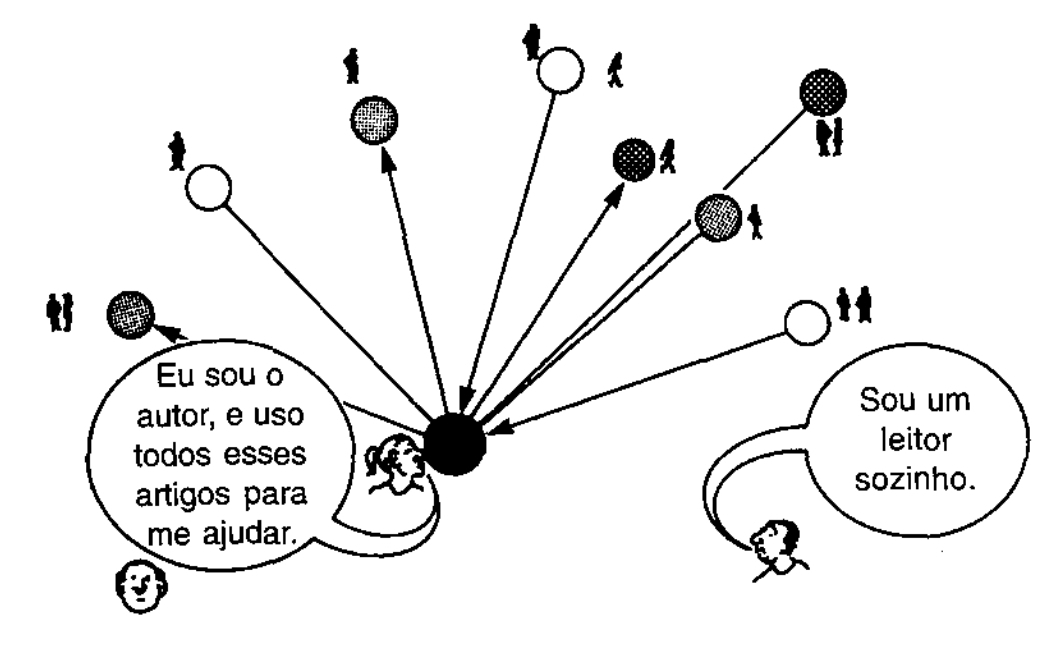
\includegraphics[width=0.6\linewidth]{figuras/cap.2/latour.jpg}
  \caption[O autor cercado de aliados e o leitor sozinho]{O autor cercado de aliados e o leitor sozinho. Figura~1.3 de \textit{Ciência em Ação}.}
  \label{fig:latour_aliados}
  \fonte{\textcite[p.~56]{Latour2011CienciaEmAcao}.}
\end{figure}

\begin{figure}[htbp]
  \centering
  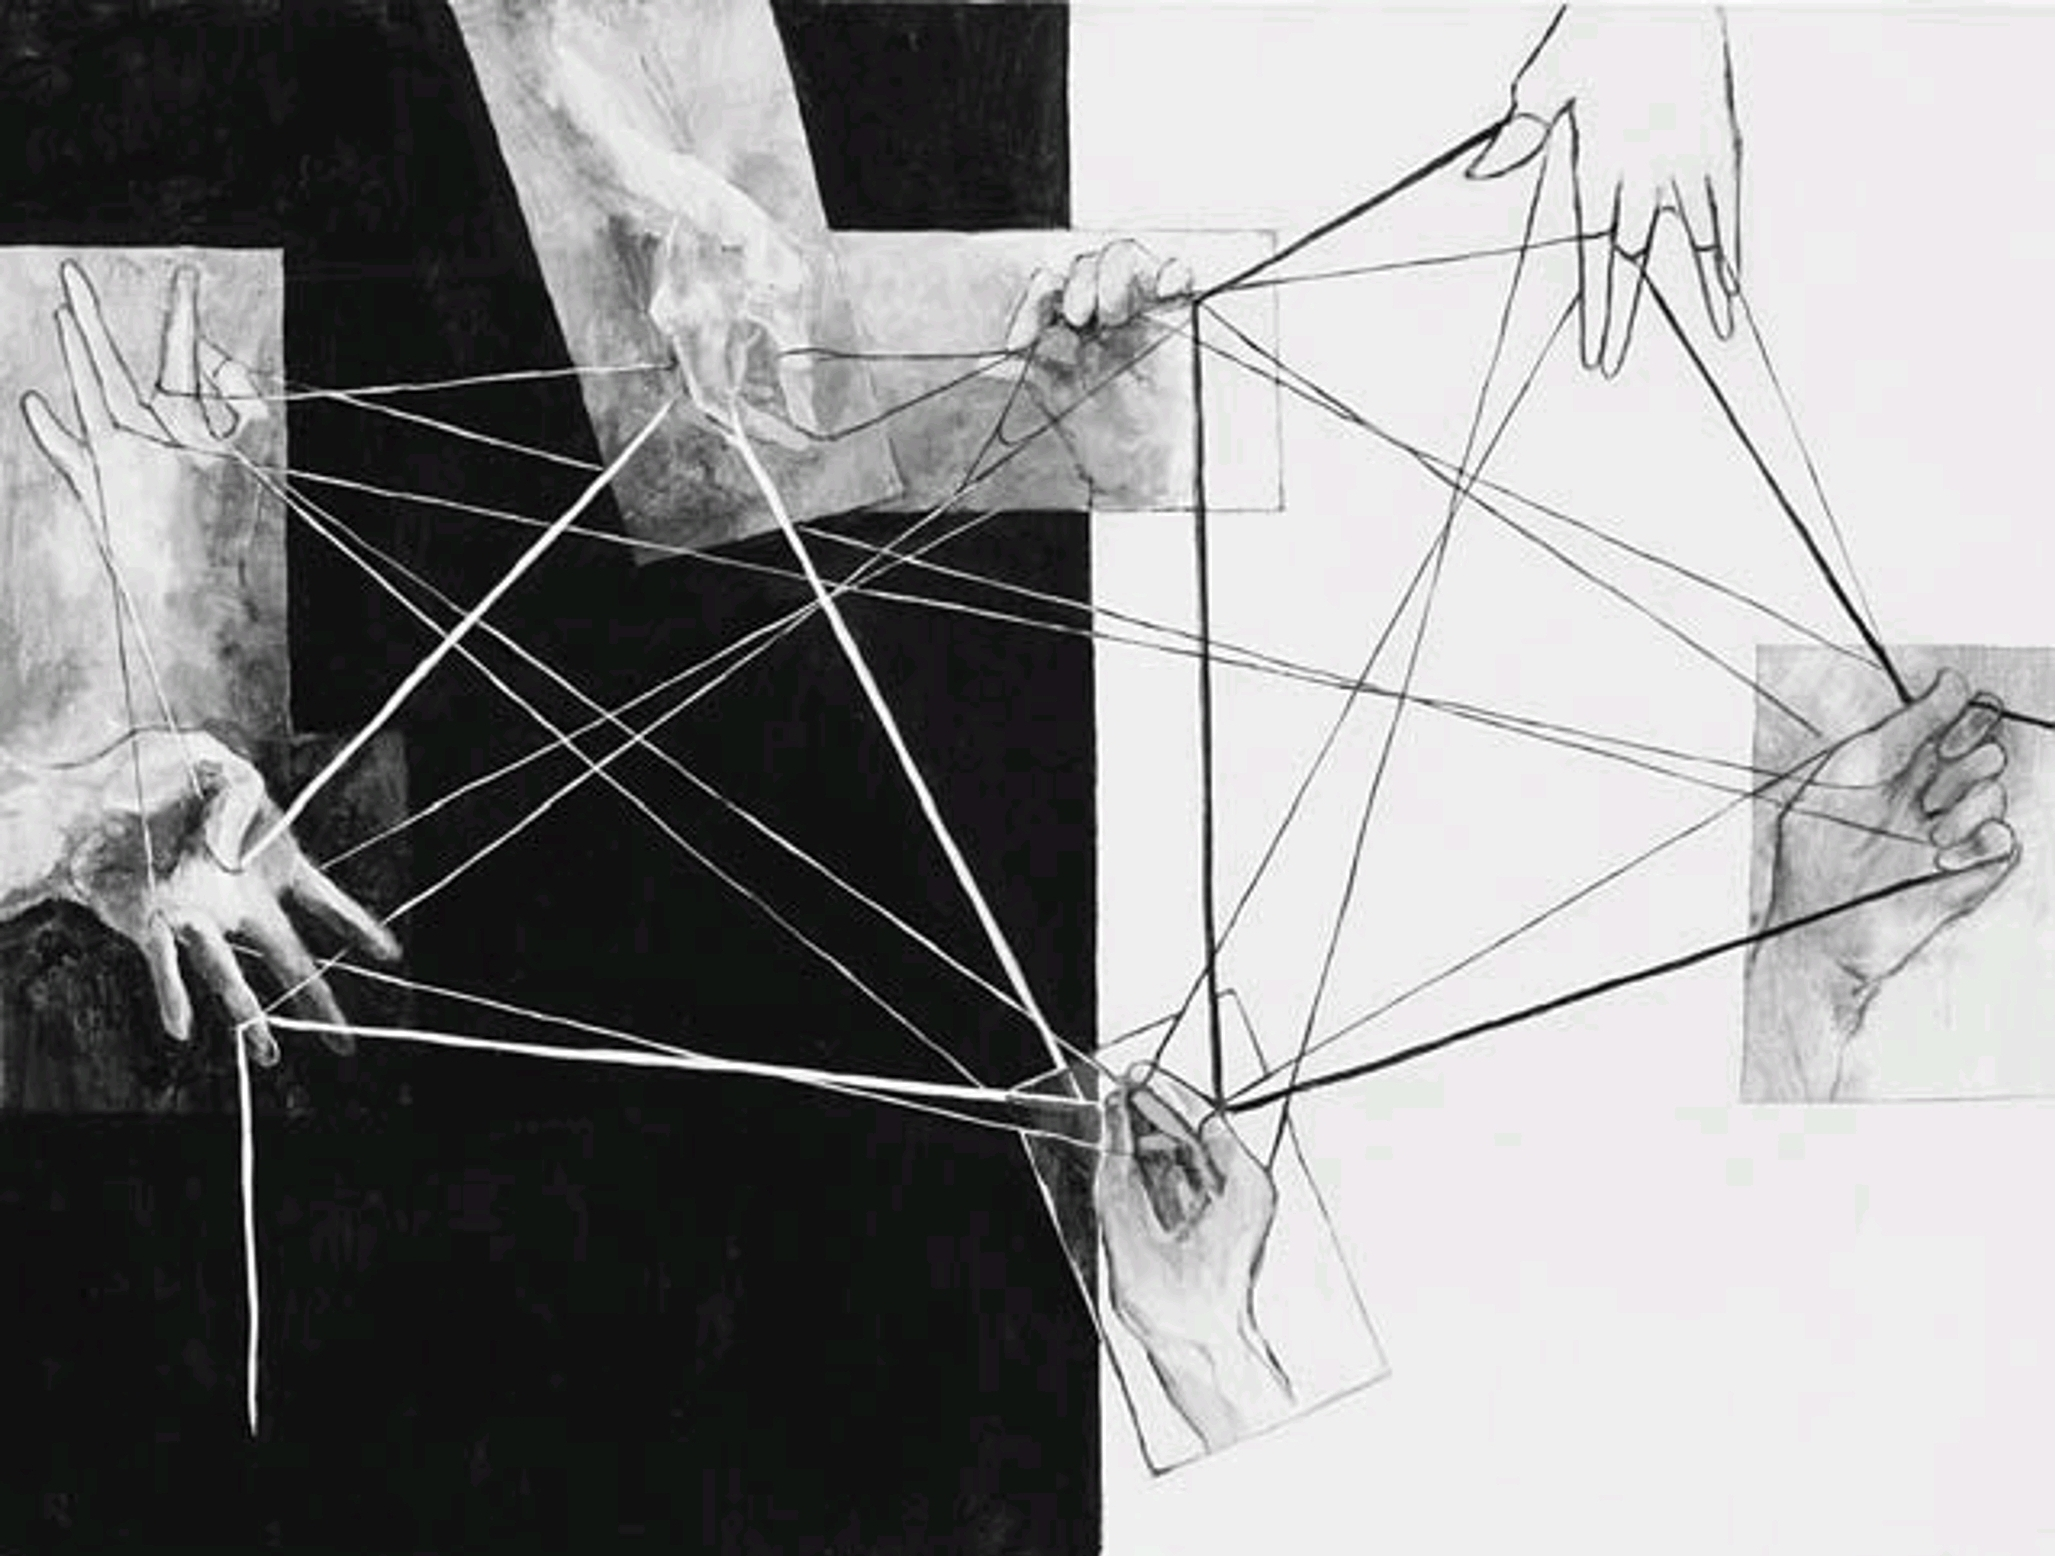
\includegraphics[width=0.6\linewidth]{figuras/cap.2/haraway.jpg}
  \caption[\textit{Cat's Cradle / String Theory}, de Baila Goldenthal]{\textit{Cat's Cradle / String Theory}, de Baila Goldenthal, 2008. Óleo sobre tela, 36~$\times$~48~pol.}
  \label{fig:goldenthal_cats_cradle}
  \fonte{\textcite[p.~35]{Haraway2016Staying}. Cortesia de Maurya Simon e Tamara Ambroson.}
\end{figure}

\epigrafe{%
Importa quais pensamentos pensam pensamentos. Importa quais conhecimentos conhece conhecimentos. importa quais relações relacionam relações. Importa quais mundos mundificam mundos. Importa quais estórias contam estórias. As pinturas de Baila Goldenthal dão um testemunho eloquente da importância dessas matérias.}%
{Donna Haraway, \textit{Ficar com o problema: fazer parentesco no Chthuluceno.}, 2016, p.~69}%

\section{}

Neste capítulo~\ref{capitulo2} retomo o conceito de tecnoetnografia que apresentei no capítulo~\ref{capitulo1}. A tecno-etnografia, conforme defini no capítulo anterior, é um conceito que surge da indissociabilidade entre escrita, análise e técnicas que desenvolvi nesta pesquisa \textit{sobre} e \textit{com} inteligência artificial, e desdobra-se em quatro capítulos, ou quatro tramas --- o capítulo~\ref{capitulo1} apresenta a tecno-etnografia como conceito e prática \textit{junto com}, \textit{junto a} e \textit{sobre} a inteligência artificial para inscrever e descrever as redes tecnocientíficas e sociotécnicas desta tese. O capítulo~\ref{capitulo3} desdobra a tecno-etnografia sobre o \texttt{C4AI} como rede em que \texttt{USP}, \texttt{FAPESP} e \texttt{IBM} são nós de uma trama sociotécnica que atravessa mais de um século de história, e o capítulo~\ref{capitulo4} desdobra-a a partir da investigação de um sistema de inteligência artificial, o \texttt{Spira}, também \textit{junto a} inteligência artificial.

% [NOTA DE REVISÃO 1] Frase final do parágrafo realinhada à formulação revisada nos capítulos 0, 1 e 3: removido "mostra apenas a forma", que rebaixava o mapa a exibição passiva; o mapa também põe em relação, em plano próprio, e nenhum dos dois planos se reduz ao outro. Corrigido de passagem o "que as teço" (redundância pronominal) para "que teço". O restante do parágrafo permanece intacto.
Situo agora sobre o que se trata este capítulo~\ref{capitulo2}. Faço uma revisão da literatura em duas linhas de análise, a análise lexicométrica das figurações na obra de Latour e de Latour e Woolgar e a análise bibliométrica do campo brasileiro e internacional de estudos envolvendo a inteligência artificial nas ciências humanas e sociais, e entre as duas recolho as leituras que cada problema empírico do meu campo evocou, dos estudos da ciência e da tecnologia às genealogias críticas do poder tecnocientífico. O mapa da Figura~\ref{fig:mapa-cap2} dá a ver a estrutura geral deste capítulo: os fundamentos que o sustentam, as seções e subseções com os autores e achados que as ocupam, as relações que as ligam, e o arremate que mantém em aberto a tensão entre alistar aliados com Latour, tecer tramas com Haraway, e propor alianças com Stengers. O diagrama pertence ao registro da inscrição, e põe em uma superfície bidimensional, de uma só vez, aquilo que o texto só pode percorrer em sequência, página após página. Reúno ainda, na linha do tempo da Figura~\ref{fig:linha-tempo-cap2}, as tradições teóricas que recolho ao longo do capítulo e o ponto em que esta tese se insere entre elas, dispostas pela data de seus marcos. Reencontro aqui a tensão que abro na Apresentação e desdobro no capítulo~\ref{capitulo1}: a urdidura, a trama e as texturas como figuras do pensamento que teço ao longo dos capítulos, no tempo e na espessura da escrita, e o mapa como o plano em que essas mesmas relações se inscrevem e fazem aparecer ligações que a leitura sequencial não alcança. Os dois planos põem em relação, cada um à sua maneira, e nenhum se reduz ao outro.

\begin{figure}[htbp]
  \centering
  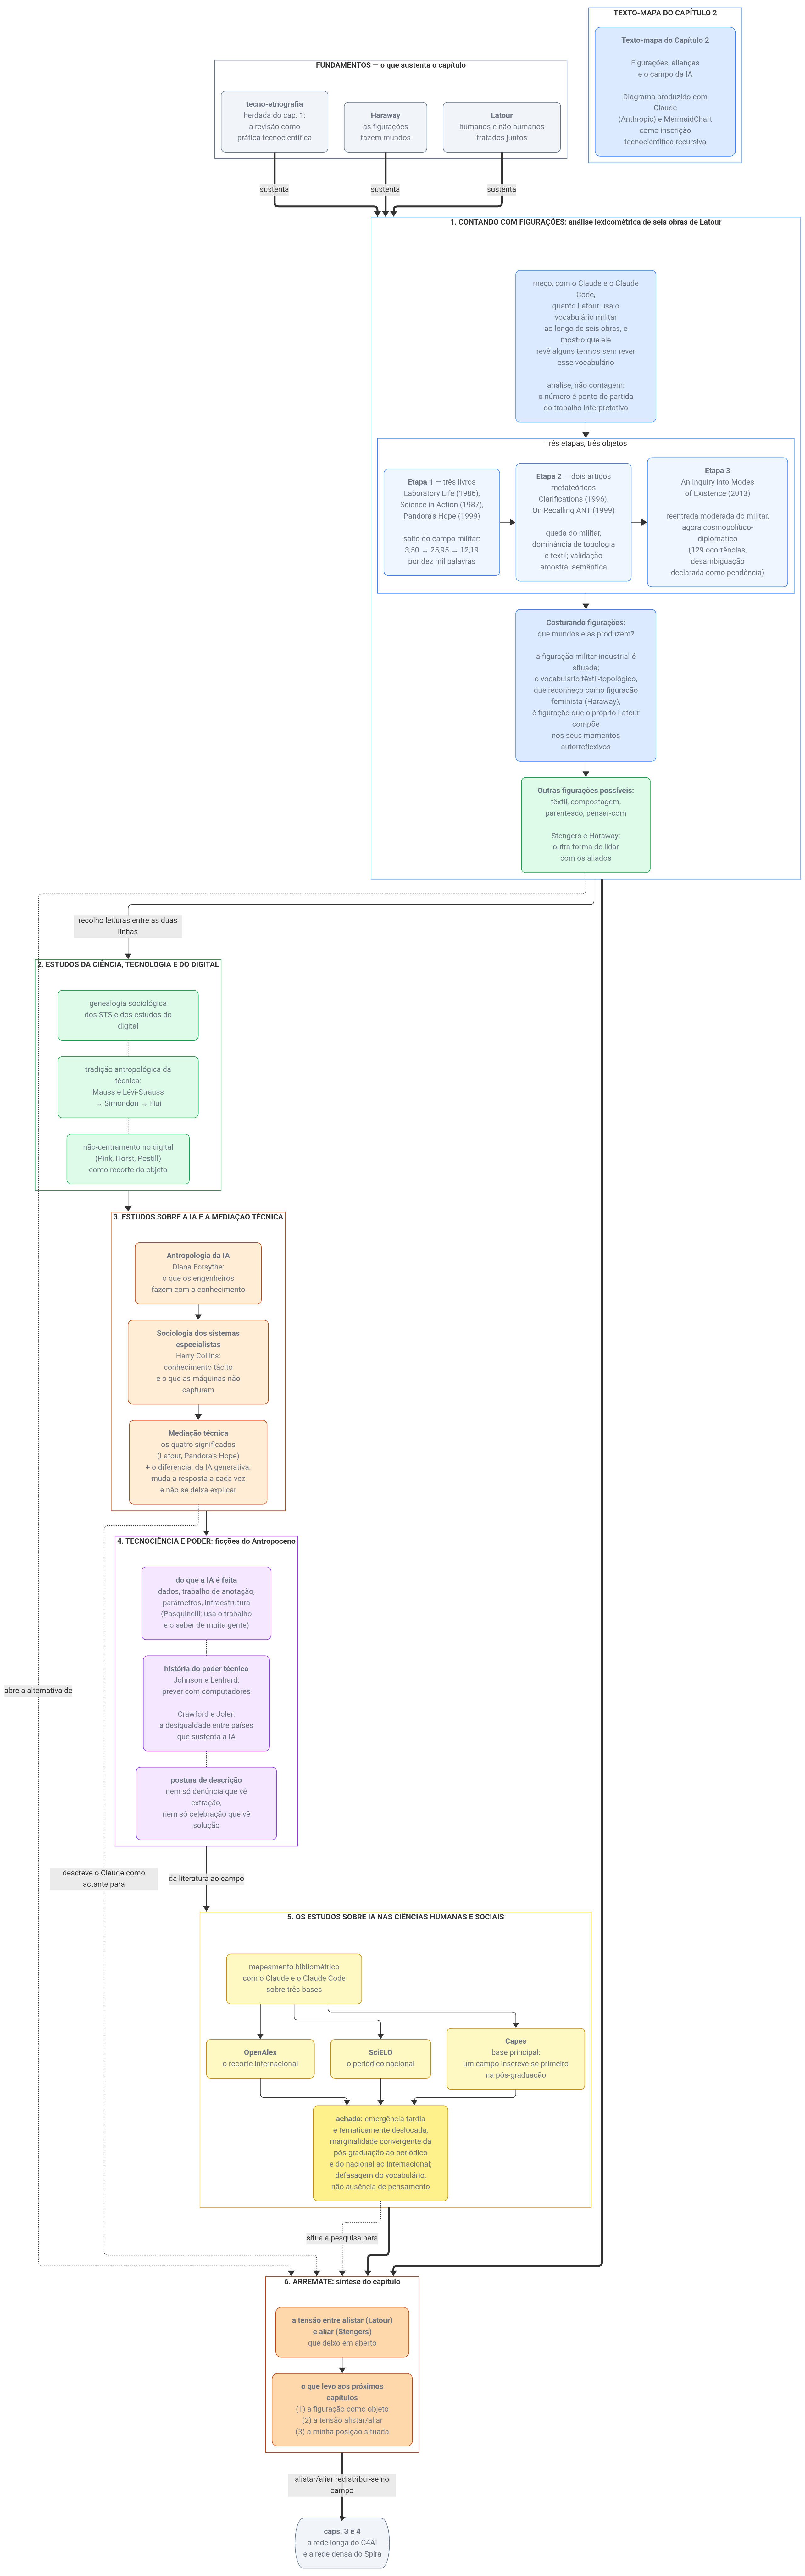
\includegraphics[width=0.3\linewidth,keepaspectratio]{figuras/cap.2/diagramas/mapa-capitulo2.png}
  \caption[Mapa do capítulo~\ref{capitulo2}]{\textbf{Mapa do capítulo~\ref{capitulo2}: a análise lexicométrica, as leituras do campo e o mapeamento bibliométrico.} Este mapa situa o leitor no percurso do capítulo, ao dar a ver em uma superfície plana as suas seções e subseções, os autores e achados que as ocupam, e as relações que as ligam, com os fundamentos que as sustentam na base: a ideia de Haraway de que as figurações fazem mundos, o tratamento de humanos e não humanos em pé de igualdade que recolho de Latour, e a tecno-etnografia que herdei do capítulo~\ref{capitulo1}. A primeira seção é a análise lexicométrica que desenvolvi com o \texttt{claude} e o \texttt{claude code}, em que meço quanto Latour usa o vocabulário militar ao longo de seis obras e mostro que ele revê alguns dos seus termos sem rever esse vocabulário, e que se desdobra em três subseções, sobre o corpus estendido dos dois artigos metateóricos, sobre a figuração em \emph{An Inquiry into Modes of Existence}, e sobre as figurações que produzem outros mundos (a têxtil, a compostagem, o parentesco e o pensar-com, com Stengers e Haraway). A segunda seção situa a pesquisa nos estudos da ciência, da tecnologia e do digital, com a tradição antropológica da técnica de Mauss e Lévi-Strauss a Simondon e Hui. A terceira trata da inteligência artificial e da mediação técnica, em três subseções, sobre a antropologia de Diana Forsythe, sobre a sociologia dos sistemas especialistas de Harry Collins, e sobre os quatro significados de mediação que Latour assenta em \emph{A Esperança de Pandora} e aquilo que a inteligência artificial generativa tem de diferente. A quarta seção descreve do que a inteligência artificial é feita, dos dados e do trabalho de anotação aos parâmetros e à infraestrutura, com Pasquinelli, Johnson e Lenhard, Crawford e Joler, e a desigualdade entre países que sustenta esses sistemas. A quinta mapeia o campo brasileiro de estudos em inteligência artificial nas ciências humanas, a partir das bases da \texttt{Capes} e do \texttt{SciELO} e do contexto internacional do \texttt{OpenAlex}, e mostra um campo recente em que a antropologia ainda comparece pouco. O arremate mantém em aberto a tensão entre alistar, com Latour, e aliar, com Stengers, e leva aos capítulos seguintes três coisas que retomo adiante, a figuração como objeto, essa tensão e a minha posição situada. A inscrição é, ela mesma, parte do que descreve, e funciona, no sentido de \textcite{Latour1986Visualization}, como móvel imutável que reúne em uma só superfície o que o texto desdobra ao longo de dezenas de páginas. Diagrama disponível em versão interativa em: \url{https://mermaid.ai/d/b4a7d089-3a37-4ab6-8e45-fc4ecca9e22f}}
  \label{fig:mapa-cap2}
\end{figure}

\begin{figure}[htbp]
  \centering
  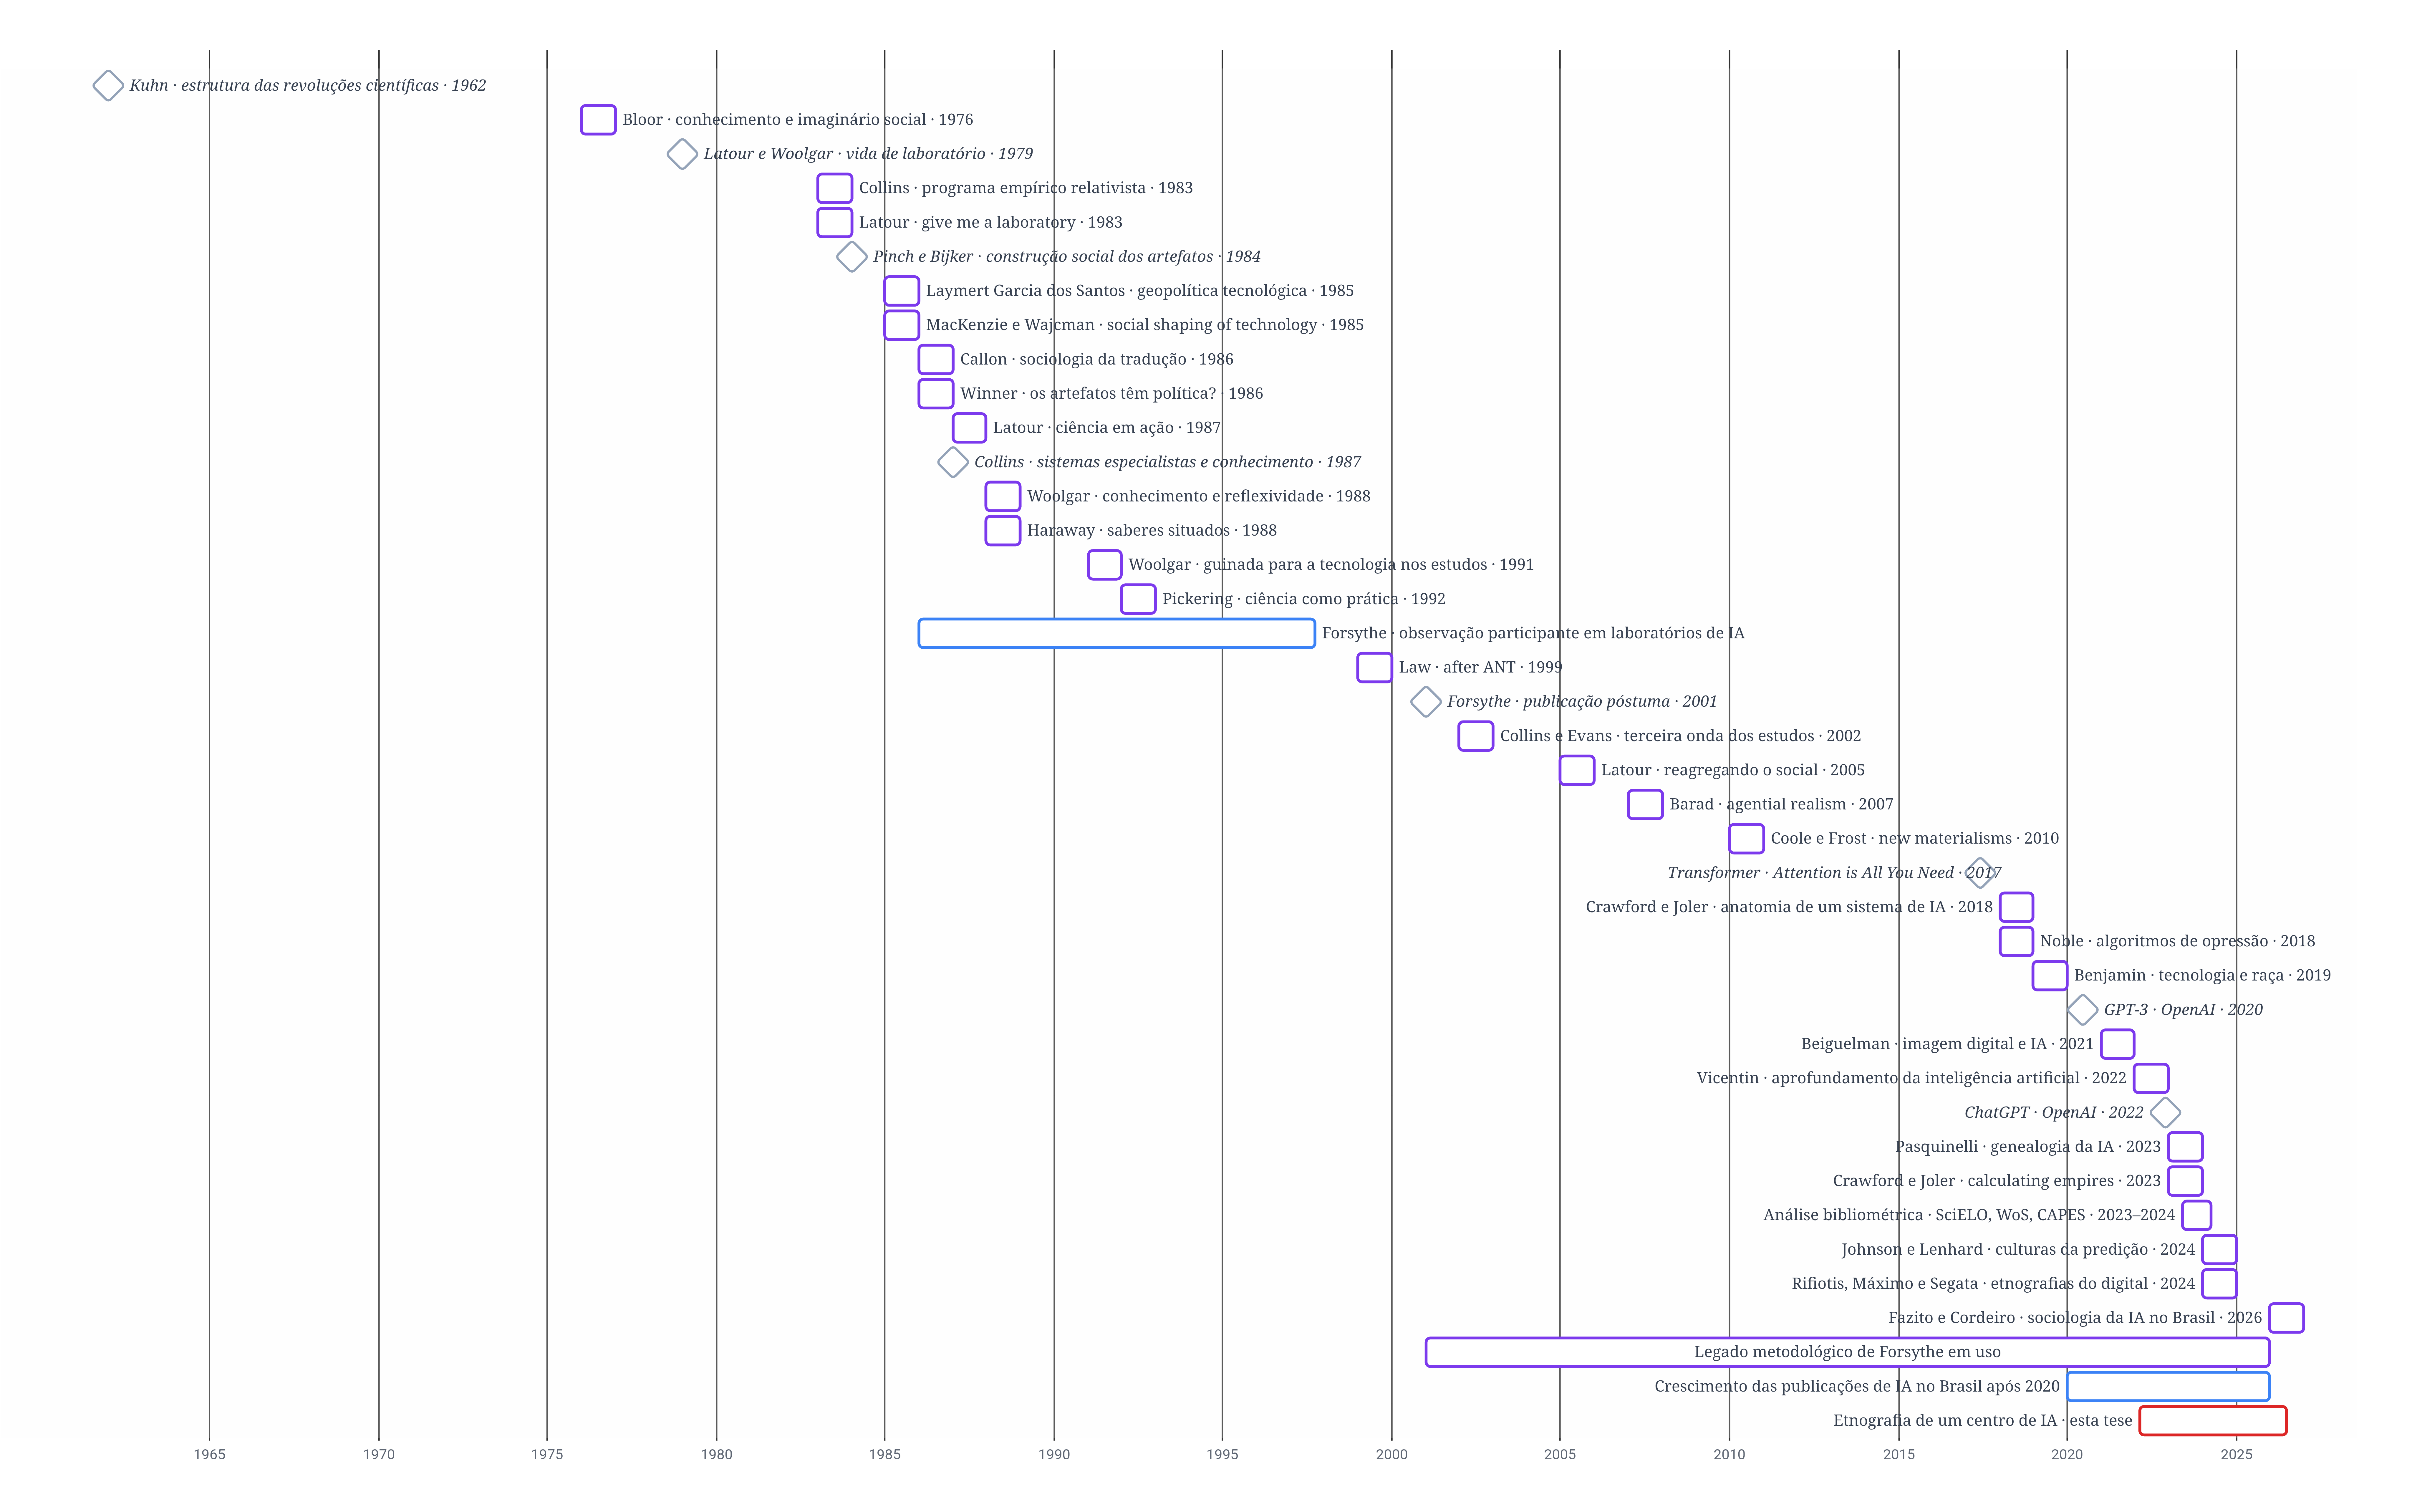
\includegraphics[width=0.85\linewidth,keepaspectratio]{figuras/cap.2/diagramas/linha-tempo-capitulo2.png}
  \caption[Linha do tempo do capítulo~\ref{capitulo2}]{\textbf{Linha do tempo do capítulo~\ref{capitulo2}: as tradições teóricas que recolho e o ponto em que esta tese se insere.} Esta linha do tempo dá a ver, em uma superfície plana, as obras das tradições de pesquisa que recolho neste capítulo, dispostas em sequência pela data de seus marcos, e pertence ao registro da inscrição, no sentido de \textcite{Latour1986Visualization}. O percurso vai da sociologia do conhecimento científico, de \textcite{Kuhn2012Structure} e \textcite{Bloor2009Conhecimento}, à construção social da tecnologia, aos estudos de laboratório e à teoria ator-rede, de \textcite{Latour1997VidaLaboratorio} a \textcite{Latour2007Reassembling}, aos novos materialismos de \textcite{Haraway1991Situated} a \textcite{Coole2010NewMaterialisms}, às etnografias de inteligência artificial de \textcite{Collins2012Expert} e \textcite{Forsythe2001}, às genealogias críticas do poder tecnológico de \textcite{Crawford2018Anatomy} a \textcite{JohnsonLenhard2024}, e ao campo emergente no Brasil, de \textcite{Santos_2022_SociologiaNaoAutocratica} e \textcite{Vicentin_2022_Esboco} a \textcite{Rifiotis2024Etnografias} e \textcite{FazitoCordeiro2026Sociologia}. Três marcos da inteligência artificial generativa atravessam essa produção e situam o leitor quanto ao momento em que a tecnologia que observo em campo emerge: o artigo do \textit{Transformer} em 2017, o \texttt{GPT-3} em 2020 e o \texttt{ChatGPT} em 2022. As duas barras em vermelho marcam onde esta tese se insere: no prolongamento da construção social da tecnologia e como etnografia de um centro de inteligência artificial, entre 2022 e 2026. Diagrama disponível em versão interativa no \texttt{MermaidChart}\footnote{Versão interativa do diagrama disponível em: \url{https://mermaid.ai/d/a7b611c1-a522-41da-9603-0a8be61de483}. Acesso em: \today.}, em que cada obra que o texto percorre em sequência se dispõe ao lado das demais em uma só superfície.}
  \label{fig:linha-tempo-cap2}
\end{figure}

A trama tecnoetnográfica deste capítulo se desdobra em duas linhas onde o conceito de tecno-etnografia é tensionado por meio de suas práticas. A primeira é a análise das metáforas e figurações na obra de Bruno Latour, desenvolvida com o \texttt{claude} e o \texttt{claude code}\footnote{O \texttt{claude} e o \texttt{claude code} são dois produtos da empresa \texttt{Anthropic} que dão acesso ao mesmo modelo de linguagem por interfaces distintas. O \texttt{claude} é a interface de conversação, em janela de \emph{chat} acessível pelo navegador ou por aplicativo, em que a interação se dá por texto, e é o ambiente em que fiz a maior parte da escrita e da discussão dos argumentos desta tese. O \texttt{claude code} é a interface de linha de comando, executada no terminal do computador, em que o modelo tem acesso direto ao sistema de arquivos e pode ler, escrever e executar \emph{scripts}, rodar programas em \texttt{Python} e versionar repositórios sem que eu precise copiar trechos de código entre janelas. As duas linhas de análise deste capítulo recorreram às duas interfaces conforme a tarefa: o processamento de arquivos extensos e a execução repetida de \emph{scripts} foram feitas no \texttt{claude code}, e a discussão dos resultados e a redação combinaram as duas. Sempre que nomeio uma delas em específico ao longo da tese, a escolha registra qual ambiente técnico mediou a tarefa descrita.} a partir de seis livros e artigos publicados entre 1986 e 2013.\footnote{O repositório com os textos normalizados, o catálogo de termos, os \emph{scripts} de extração e contagem em \texttt{Python}, as planilhas de validação e os \emph{outputs} de cada etapa está disponível em \url{github.com/julianehelanski/analise-figuracoes-latour}. Os PDFs das obras de Latour ficam fora do repositório por razões de direitos autorais.} A segunda é o mapeamento da emergência do campo brasileiro de estudos em inteligência artificial nas ciências humanas e sociais, realizado por análise bibliométrica das plataformas \texttt{SciELO} e \texttt{Capes} com o \texttt{claude} e o \texttt{claude code}, com tratamento e visualização de dados em \texttt{Python} no ambiente de programação para análise de dados \texttt{Spyder/Anaconda}.\footnote{O repositório com todos os dados dessa analise está disponível em \url{https://github.com/julianehelanski/analise_bibliometrica_ia_ciencias_humanas}.}
        
Ao disponibilizar publicamente os repositórios do \texttt{GitHub} com os \emph{scripts}, os catálogos, as planilhas de validação e os \emph{outputs} de cada etapa de análise, incluo essa prática comum da ciência de dados e da computação\footnote{O repositório do \texttt{GitHub} permite armazenar e publicar os códigos, os \textit{scripts}, um tipo específico de código criado para automatizar tarefas repetitivas, e os dados utilizados em um estudo, e retornar a qualquer versão anterior do projeto. A publicação desses arquivos permite que outras pesquisadoras verifiquem os resultados e reproduzam a análise.} também como uma prática tecnoetnográfica. A análise em linguagem de programação \texttt{Python}, a automatização da análise textual, as buscas padronizadas nas plataformas de indexação bibliográfica e as sessões recursivas com o \texttt{claude} e o \texttt{claude code} são técnicas em sentido estrito, e são técnicas que podem ser reexecutadas, contestadas ou refinadas a partir dos repositórios públicos. Essas técnicas são parte da pesquisa e do trabalho relacional e situado que transforma os meios, os modos e os resultados que a pesquisa alcança.

O mapeamento bibliométrico que realizei tem por base principal o Catálogo de Teses e Dissertações da \texttt{Capes}, complementado por uma sondagem na biblioteca eletrônica \texttt{SciELO} e pela comparação com a base internacional \texttt{OpenAlex}. Tomei o Catálogo da \texttt{Capes} como base porque o que me interessa é o momento de formação de um campo nas ciências humanas e sociais brasileiras, que se inscreve primeiro na pós-graduação, na tese e na dissertação, antes de chegar ao artigo publicado em periódico. A \texttt{SciELO} e o \texttt{OpenAlex} situam esse campo brasileiro emergente diante da produção em periódico, nacional e internacional. A seção~\ref{sec:emergencia_campo_brasileiro} apresenta esse mapeamento e detalha a escolha das bases, os protocolos de classificação que adotei e os resultados a que cheguei. 

A seção~\ref{sec:analise_lexicometrica} apresenta a análise das metáforas e figurações em Latour, e em Latour e Woolgar, em três etapas: a etapa~1 processou três livros (\emph{Laboratory Life}, de Latour e Woolgar, 1986, \emph{Science in Action} 1987, \emph{Pandora's Hope} 1999); a etapa~2 estendeu a análise a dois artigos metateóricos (\emph{Clarifications} 1996, \emph{On Recalling ANT} 1999);  a etapa~3 processou \emph{An Inquiry into Modes of Existence} (2013). Chamo metateóricos os dois textos da etapa~2 porque nenhum deles descreve um caso, como fazem os três livros da etapa~1, e ambos tomam por objeto a própria teoria ator-rede, que revisam e esclarecem.\footnote{\emph{On Recalling ANT} é um capítulo da coletânea \textit{Actor Network Theory and After}, organizada por John Law e John Hassard \parencite{LawHassard1999ANTAfter}. \emph{Clarifications} circula como \emph{working paper} sem paginação editorial estável, e há versão publicada na revista \textit{Soziale Welt}, vol.~47, 1996, p.~369--381; cito o \emph{working paper} por ser a versão sobre a qual fiz a extração para a análise, pela paginação interna do arquivo versionado no repositório público.} A distinção é minha, recolhida para organizar os dados da análise, e a faço porque a etapa~2 examina como as figurações de Latour se comportam quando o que ele descreve deixa de ser um laboratório ou um cientista e passa a ser a sua própria teoria. É nesses dois textos, e sobretudo em \emph{On Recalling ANT}, que Latour revê alguns dos seus termos sem rever a figuração militar, que é o achado que a análise sustenta. Entre essa seção e a do mapeamento bibliométrico, percorro as leituras que atravessei ao longo do doutorado e que registraram, em diferentes momentos da pesquisa, as interlocuções teóricas que cada problema empírico do meu campo evocou: as primeiras pesquisas antropológicas e sociológicas sobre inteligência artificial (Diana Forsythe, Harry Collins), o conceito de mediação técnica que Latour formula em \emph{Pandora's Hope} revisitado à luz dos sistemas de inteligência artificial generativa, os estudos de engenharia e culturas da predição (Ann Johnson, Johannes Lenhard), e as genealogias críticas do poder tecnocientífico (Kate Crawford, Matteo Pasquinelli, Vladan Joler), em diálogo com as inflexões brasileiras dessas perguntas em Laymert Garcia dos Santos, Diego Vicentin, Pedro Ferreira Peixoto e Giselle Beiguelman. A análise lexicométrica e o mapeamento bibliométrico parecem dois temas distintos, mas se tecem na mesma trama: a figuração de Latour, a do recrutamento de aliados, é o gancho pelo qual ampliei o escopo da primeira análise à segunda, porque mapear um campo em emergência, e nele situar o meu próprio trabalho, é também um gesto de pôr-em-relação.

As referências que reúno neste capítulo~\ref{capitulo2}, como as do capítulo~\ref{capitulo1}, atravessam direta ou indiretamente a descrição que faço do \texttt{C4AI} e do \texttt{Spira} nos capítulos~\ref{capitulo3} e~\ref{capitulo4}. O capítulo~\ref{capitulo3} investiga o \texttt{C4AI} ao longo de cinco anos de parceria \texttt{USP}-\texttt{FAPESP}-\texttt{IBM}, do convênio inicial em outubro de 2020 ao encerramento em dezembro de 2025, com a trajetória corporativa da \texttt{IBM} desde 1890; o capítulo~\ref{capitulo4} acompanha o sistema de inteligência artificial \texttt{Spira} e suas inscrições tecnocientíficas. Em ambos, a tecno-etnografia que ensaio nesta tese funciona quando as figurações que apresento neste capítulo~\ref{capitulo2} participam da descrição etnográfica e quando a pesquisa que realizo com o \texttt{claude} e o \texttt{claude code} passa a fazer parte da pesquisa como uma prática tecnocientífica.

Justifico o recorte do corpus, isto é, por que tomei essas seis obras para a análise lexicométrica e não outras, ou por que não a complementei com as demais. O recorte não foi montado para a análise lexicométrica, ele a antecede. Esta tese partiu da teoria ator-rede e, dentro dela, de três obras de Latour, \emph{Laboratory Life}, \emph{Science in Action} e \emph{Pandora's Hope}, e de modo particular de \emph{Science in Action}, obra com a qual o próprio título desta tese dialoga. A figuração militar-industrial que rastreio já era objeto da pesquisa antes de qualquer contagem, sustentada pela leitura e utilização desses termos na construção desta tese. A análise lexicométrica veio depois, e veio para dar base à leitura interpretativa que eu já vinha fazendo. Foi por isso que escolhi essas três obras, e não outras, para o núcleo da análise. Os dois artigos metateóricos, \emph{Clarifications} e \emph{On Recalling ANT}, entram nesse recorte porque pertencem ao mesmo escopo de questões, o da construção e da reformulação da teoria ator-rede, e oferecem a contraparte metateórica dos três livros, em que Latour reflete sobre a própria teoria em vez de aplicá-la à descrição da ciência. A obra \emph{An Inquiry into Modes of Existence} fecha a análise como a entrada de um novo conjunto figurativo para além da teoria ator-rede. O corpus é, portanto, o conjunto de obras onde se constrói, sistematiza e reformula a teoria ator-rede. Obras posteriores, como \emph{Politics of Nature} e \emph{Down to Earth}, não entram na análise lexicométrica porque as considero pertencentes a um outro projeto de Latour, o de ecologia política, que não tomo como meu objeto neste capítulo, e que retomo de modo breve ao final desta seção para não reduzir as obras ao recorte que analiso. 

A revisão bibliográfica que faço aqui é também uma prática tecnocientífica. Comecei reunindo autoras e autores, citando a autoridade de uns ao lado das ressalvas de outros, acumulando referências que sustentassem as descrições que viriam: o gesto que \textcite[cap.~1]{Latour2011CienciaEmAcao} descreve como o modo militar da produção tecnocientífica, o de alistar aliados para vencer a controvérsia. Conforme a escrita avançava, e com ela a análise das figurações, o gesto foi se deslocando do alistar para o tecer. Distingo dois registros do que chamo relação, e não os confundo: as relações da rede que sigo em campo já estão dadas entre os atores, e o meu trabalho é reconhecê-las e segui-las, como faço no capítulo~\ref{capitulo3}; o pôr-em-relação da escrita, ao contrário, é um gesto que constituo, no sentido que tomo de Strathern, ao fazer entrarem em uma mesma relação as leituras, a análise e o que descrevo, de onde emerge o que nenhuma delas continha sozinha. É esse segundo gesto, situado e por isso responsável, que o parágrafo descreve. A figuração do alistamento descreve como a revisão começa sob o formato acadêmico, e o percurso da escrita mostra esse começo se transformando à medida que passei a tecer as referências em vez de arregimentá-las.\footnote{A figuração têxtil para pensar o próprio fazer da pesquisa não é exclusiva desta tese, e a reencontro, entre outras, na tese de \textcite{costa2024manchando}, defendida no mesmo programa de pós-graduação em ciências sociais da \texttt{Unicamp}, e na mesma linha de pesquisa, \enquote{Modos de conhecimento e suas expressões: experiências e trajetórias}. Costa figura a escrita como trabalho de tecelagem e nomeia a sua conclusão de \enquote{arremate}, o ponto com que se rematam as pontas dos fios ao fim de uma costura, e desdobra o vocabulário da trama, da urdidura e do fio que costura temas heterogêneos. A coincidência das duas escolhas, em teses contemporâneas, do mesmo lugar e da mesma linha, cujo próprio nome toma o conhecimento como algo que se tece em experiências e trajetórias, sugere que a figuração têxtil opera como um modo de pensamento partilhado no campo, e não como recurso estilístico isolado.} É esse deslocamento que o capítulo registra, e ele repete, no meu próprio percurso de escrita, a tensão entre metáforas e figurações que percorre o capítulo~\ref{capitulo1}: Latour, Haraway e Stengers aparecem aqui lado a lado, três modos que tomam o conhecimento como prática de pôr as coisas em relação e divergem no que essa relação persegue. Em Latour, alistar aliados para vencer a controvérsia; em Haraway, tecer tramas multiespécies; em Stengers, fazer alianças com cientistas e engenheiros e desacelerar o pensamento para resistir à lógica capitalista.

Abro o capítulo~\ref{capitulo2} com duas epígrafes e duas figuras postas em tensão. A epígrafe de Latour e a Figura~\ref{fig:latour_aliados} enunciam, ou evocam, uma figuração que atravessa \textit{Ciência em Ação}. \enquote{Alistar} designa, em português como em francês (\textit{enrôler}), recrutar para um exército. Os \enquote{aliados} são os que se alinham do mesmo lado à frente, o \textit{front}. As \enquote{provas de força} decidem controvérsias por enfraquecimento sucessivo das posições adversárias. As \enquote{referências bibliográficas} funcionam como \enquote{escolta protetora} de um texto que, sem elas, seria como \enquote{Uma monografia sem referencias é como uma criança desacompanhada a caminhar pela noite de uma grande cidade que ela não conhece: isolada, perdida, pode acontecer-lhe qualquer coisa.} \parencite[p. 48]{Latour2011CienciaEmAcao}. O artigo científico é descrito como \enquote{máquina de guerra} cuja eficácia se mede pelo número e qualidade dos reforços que consegue arregimentar contra o adversário. A retórica é militar; a economia, agonística; a figuração dominante, a do exército que avança \parencite[p.~53, e cap.~1 em geral]{Latour2011CienciaEmAcao}. A própria Figura~1.3 de \textit{Ciência em Ação} dá a essa figuração a sua forma visual: um autor cercado de aliados de um lado, um leitor sozinho do outro, e a discordância tornada custosa pelo número dos reforços alinhados. Em \textit{A Esperança de Pandora}, esse mesmo vocabulário se sistematiza no que Latour chama de terceiro circuito da circulação científica, \enquote{Alianças (aliados)}, e se exemplifica pela capacidade de atrair o interesse dos militares para a física, dos industriais para a química, dos reis para a cartografia \parencite{Latour2017Esperanca}.\footnote{A linguagem militar atravessa o capítulo~1 (\enquote{Literatura}) de \textit{Ciência em Ação} de modo sistemático. Latour define a retórica científica como a capacidade de \enquote{Afirmo, ao contrário, que deveremos vir a chamar de científica a retórica capaz de mobilizar para um só ponto mais reforços do que as antigas.}\parencite[p. 92]{Latour2011CienciaEmAcao} retóricas, que se limitavam a aliados externos como a paixão ou o estilo. O artigo científico permite ao autor escrever acompanhado de um exército de outros textos e autores. As referências bibliográficas funcionam como escolta protetora. Um texto carregado de notas força o adversário a enfraquecer cada um dos aliados recrutados antes de atingir a afirmação central. A força de um argumento cresce quando os reforços, figuras, tabelas, gráficos, são ostentados no próprio corpo do texto, formando camadas defensivas que tornam a discordância custosa. Latour observa ainda que, embora Galileu sustentasse que um homem sozinho com a verdade poderia vencer mil autoridades, na prática da ciência em construção o vencedor é quem consegue arregimentar o maior número de aliados bem alinhados. Os termos \enquote{provas de força}, \enquote{contingente}, \enquote{estratégias e táticas} e \enquote{equilíbrio de forças} distribuem-se ao longo do mesmo capítulo, tratando a tecnociência como parte de uma máquina de guerra cujo objetivo é vencer a controvérsia \parencite[p.~53]{Latour2011CienciaEmAcao}.} A epígrafe de Haraway e a Figura~\ref{fig:goldenthal_cats_cradle} enunciam uma figuração da trama e das linhas. A repetição das palavras em \enquote{Importa quais estórias contam estórias} faz da própria sintaxe a forma do pensamento: importa com que histórias se contam histórias, com que figurações se figuram figurações, e a frase se enrola sobre si como o fio que a descreve. A figuração aqui é a do \textit{cat's cradle}, o jogo do berço de gato, em que um par de mãos passa o fio a outro par e a forma só se sustenta enquanto há quem a receba e devolva. A pintura de Baila Goldenthal que Haraway escolhe para a página, \textit{Cat's Cradle/String Theory}, dá a essa figuração a sua forma visual: mãos entrelaçadas por um fio compartilhado, sem front, sem adversário, sem reforços a arregimentar.\footnote{A figuração têxtil atravessa \textit{Ficar com o problema} de modo tão sistemático quanto a figuração militar atravessa o \textit{Ciência em Ação} de Latour. A figura de barbante (\textit{string figure}) dá título ao primeiro capítulo e organiza o livro inteiro. Haraway descreve o brincar com figuras de barbante: \enquote{Brincar com figuras de barbante tem a ver com dar e receber padrões, com soltar os fios e falhar, mas, às vezes, encontra-se algo que funciona, algo consequente e talvez até mesmo belo, que não estava ali antes} \parencite[p.~24]{Haraway2023Ficar}. E insiste em um ponto que distingue essa figuração da do alistamento: \enquote{As figuras de barbante exigem que se fique parado para receber os fios e passar adiante os padrões. Esses jogos podem ser feitos por muitos seres, com quaisquer tipos de extremidade, contanto que o ritmo entre dar e receber seja sustentado. O conhecimento e a política também são feitos assim, ao se passarem adiante os fios em torções e meadas que exigem paixão e ação, deter-se e mover-se, ancorar e dar partida} \parencite[pp.~24--25]{Haraway2023Ficar}. O jogo do berço de gato, portanto, não acumula reforços, e a sua forma se desfaz quando um dos parceiros retém o fio em vez de devolvê-lo: a figura só persiste enquanto o ritmo de dar e receber se mantém. A essa figuração do fio soma-se a da \textit{sympoiesis}, o fazer-com que Haraway apresenta como palavra-chave do segundo capítulo \parencite{Haraway2023Ficar}, e contra o qual contrasta o individualismo delimitado que considera não mais pensável. Os termos fio, nó, emaranhado, padrão, trama, distribuem-se por todo o livro, e a própria frase da epígrafe pertence a uma série de repetições da mesma estrutura, em que Haraway desdobra um princípio que credita a Marilyn Strathern, o de que importa com que ideias se pensam outras ideias \parencite{Haraway2023Ficar}.}

Como essas figurações aparecem na obra de Latour? Em \textit{On recalling ANT}, ele reconhece a \enquote{pobreza ridícula do vocabulário da TAR} e explica que essa pobreza foi uma escolha deliberada. Os termos da TAR, associação, translação, aliança, ponto de passagem obrigatório, eram, escreve Latour, um sinal claro de que nenhuma dessas palavras deveria substituir o vocabulário rico da prática do próprio ator, e funcionavam apenas como um modo de evitar sistematicamente que a sociologia, a metafísica e a ontologia dos atores fossem substituídas pelas dos cientistas sociais. Ao nomear o trabalho do pesquisador, Latour recusa inclusive o verbo \enquote{estudar}, e prefere a perífrase \enquote{conectar-se com eles através de algum protocolo de pesquisa}, porque, em suas palavras, os pesquisadores da TAR não podem propriamente ser ditos \enquote{estudar} os outros atores sociais.\footnote{No original: \enquote{The ridiculous poverty of the ANT vocabulary---association, translation, alliance, obligatory passage point, etc.---was a clear signal that none of these words could replace the rich vocabulary of the actor's practice, but was simply a way to systematically avoid replacing their sociology, their metaphysics and their ontology with those of the social scientists who were connecting with them through some research protocol---I use this cumbersome circumlocution to avoid the loaded term \enquote{studying}, because ANT researchers cannot exactly be said to \enquote{study} the other social actors} \parencite[p.~20]{Latour1999RecallingANT}. A tradução no corpo é minha.}. Mais adiante, compara o método da teoria ator-rede (TAR) a uma metáfora de modo explícito: \enquote{I have often compared it to perspective drawing [\ldots] I am well aware of the limits of this metaphor since there is hardly a more constraining method than three dimensional perspectival drawing} \parencite[p.~21]{Latour1999RecallingANT}. Em \textit{On actor-network theory: a few clarifications}, ele diz: \enquote{Put too simply AT is a change of metaphors to describe essences: instead of surfaces one gets filaments} \parencite[p.~2]{latour1996clarifications}.\footnote{A categoria \enquote{metáfora} que Latour assume aqui tem uma história na filosofia da ciência que recupero brevemente para sustentar o argumento que continuo a costurar. Mary Hesse, em \textit{Models and Analogies in Science} \parencite{Hesse1965ModelsAnalogies}, formulou que toda metáfora científica funciona por três tipos de correspondência entre domínio-fonte e domínio-alvo: analogias positivas, que especificam o que de fato é mapeado entre os dois domínios; analogias negativas, que delimitam o que está explicitamente excluído do mapeamento; e analogias neutras, que marcam áreas deixadas em aberto para investigação futura. Os mapeamentos circunscrevem o que pertence à analogia positiva, e as exclusões registram uma escolha do que fica de fora. Max Black \parencite{Black2019ModelsMetaphors} acrescenta que metáforas científicas revelam e ocultam ao mesmo tempo, e modelam tanto o que se compreende de um fenômeno quanto o que permanece fora do enquadramento. Lakoff e Johnson \parencite{LakoffJohnson2008MetaphorsWeLiveBy} sustentam que esse trabalho de revelar e ocultar é constitutivo da prática teórica em qualquer campo, e que o vocabulário metafórico de uma teoria estrutura o que conta como observação relevante.} A TAR exige, ainda, \enquote{uma postura polêmica firme} (\textit{a strong polemical stance}), reconhece Latour, \enquote{to forbid the analyst to dictate actors what they should do} \parencite[p.~7]{latour1996clarifications}. Todavia, o que Latour não submete ao mesmo escrutínio é a especificidade da figuração que escolheu, a militar-industrial, e as consequências dessa escolha para o que se deixa descrever e para o que escapa à descrição quando essa figuração é utilizada. 

Ainda em \textit{On recalling ANT}, ao apresentar o que descreve como \enquote{o terceiro prego no caixão dos termos da teoria}, Latour formula uma autocrítica que intensifica a análise sobre as figurações e para as evidências quantitativas que apresento na seção~\ref{sec:analise_lexicometrica}: \enquote{I agree that we have not always been true to the original task, and that a great deal of our own vocabulary has contaminated our ability to let the actors build their own space, as many critiques have charitably shown} \parencite[pp.~19--20]{Latour1999RecallingANT}.\footnote{A análise refinada da figuração militar mostra que quando Latour escreve sobre a TAR, o vocabulário militar se ausenta; quando escreve com a TAR para descrever a tecnociência, ele satura o texto. A figuração militar é, portanto, figuração de uso, não de tematização, e é precisamente por nunca ter sido tematizada por Latour que ela escapou à crítica que ele fez aos outros termos da teoria, conforme o relatório consolidado do projeto em \url{github.com/julianehelanski/analise-figuracoes-latour/blob/main/outputs/relatorio_consolidado/relatorio_figuracoes_latour.md}.} O \enquote{vocabulário} da TAR \textit{contaminou} a tarefa que essa mesma teoria reivindicava para si. No entanto, é necessário marcar o alcance dessa afirmação. Os termos que Latour menciona em \textit{On recalling ANT} são \textit{ator}, \textit{rede}, \textit{teoria} e o hífen, os quatro \enquote{pregos no caixão} que organizam o artigo, e a contaminação que ele admite é a das conotações que esses quatro termos arrastam consigo. Ao tratar do termo \textit{teoria}, Latour problematiza o próprio nome pelo qual a TAR ficou conhecida, e adverte que a TAR é \enquote{a method and not a theory, a way to travel from one spot to the next, from one field site to the next} \parencite[p.~21]{Latour1999RecallingANT}, isto é, um modo de seguir atores, e não uma teoria que os explica. Mantenho, ainda assim, a designação \enquote{teoria ator-rede} ao longo desta tese, porque é a forma pela qual o campo e o próprio Latour nomeiam o conjunto, e porque a ressalva que ele faz não desfaz o nome, e sim adverte sobre o que ele sugere. A figuração militar-industrial, no entanto, não entra nessa autocrítica. Quando os críticos apontam os problemas da figuração militar-industrial, e se referirem ao caráter \enquote{gerencial, de engenharia, maquiavélico, demiúrgico} da TAR, Latour responde que essas críticas estão \enquote{off target} \parencite[p.~16]{Latour1999RecallingANT}, e em \textit{Clarifications} diz que a crítica à TAR como uma rede de aliados homens em luta por poder como \enquote{the bottom of misunderstanding} \parencite[p.~5]{latour1996clarifications}. Latour faz uma autocrítica diferente para a teoria ator-rede ao amenizar a crítica à figuração militar que satura sua escrita desde \textit{Ciência em Ação}. Latour propõe uma maneira curiosa para \enquote{ficar com o problema}. Ele propõe empobrecer o \enquote{vocabulário} ainda mais, pois \enquote{this weakness on our part does not mean, however, that our vocabulary was too poor, but that, on the contrary, it was not poor enough, and that designing a space for the actors to deploy their own categories is a much harder task than we thought at first} \parencite[p.~20]{Latour1999RecallingANT}.\footnote{A aspiração de Latour, a de projetar um espaço em que os atores desdobrem as suas próprias categorias com o mínimo de vocabulário do analista, reencontra um problema que a antropologia já vinha tratando havia décadas sob o nome de tradução. Onde Latour busca empobrecer o vocabulário até que o ator apareça por si, a antropologia da tradução sustenta que toda descrição carrega o vocabulário situado de quem descreve, e que o encontro entre o sistema conceitual do pesquisador e o do pesquisado permanece opaco. Eduardo Viveiros de Castro dá a esse encontro o nome de equivocação controlada: traduzir é perceber os falsos homônimos, os termos que parecem dizer o mesmo e dizem outra coisa, e comunicar através da diferença, em vez de presumir univocidade \parencite{ViveirosdeCastro2018Equivocacao}. A comparabilidade direta, escreve ele, não significa tradutibilidade imediata, assim como a continuidade ontológica não implica transparência epistemológica. O problema que Latour formula como pobreza insuficiente do vocabulário é, nesses termos, o problema da equivocação que toda tradução carrega, e que se enfrenta pela assunção da posição situada de quem traduz, mais do que pela subtração de palavras, no sentido que tomo de Haraway e que sustenta a primeira pessoa desta tese. É essa assunção, e não o apagamento do vocabulário, que pratico ao rastrear na escrita de Latour a figuração militar que ele não examina.} Todavia, mesmo que com poucas e pobres palavras, tendo em vista que é melhor deixar os atores/actantes falarem por eles mesmos, não ajuda a pensar como funciona, nos efeitos ou nas consequências da figuração militar. Desse modo, a análise que sustento neste capítulo~\ref{capitulo2} busca investigar o peso, a distribuição e as correlações que a figuração militar-industrial teve/tem na realização de pesquisas tecnocientíficas, que como esta tese, buscam em Latour algum tipo de inspiração e/ou fundamentação.
 
Concordo com o diagnóstico de Latour sobre a contaminação, e dele me afasto no que diz respeito à solução. Empobrecer aquilo que o próprio Latour chama de \enquote{infralinguagem} (\textit{infralanguage}), o vocabulário mínimo que, em suas palavras, \enquote{has to be poor, limited, short and simple} \parencite[p.~\texttt{[p. 7]}]{latour1996clarifications}, reduz o número de categorias que se impõe aos atores mas deixa intacta a figuração das poucas que restam. Translação, aliança, recrutamento, ponto de passagem obrigatório seguem carregando o registro militar-industrial mesmo depois de enxugados ao mínimo, porque a figuração está naquilo que cada termo convoca, mais do que na quantidade de termos. Por isso a tarefa que assumo neste capítulo~\ref{capitulo2} desloca a pergunta de Latour, e ao invés de perguntar quantos termos compõem o seu \enquote{vocabulário}, pergunto qual figuração esse vocabulário sustenta, e o que ela torna descritível ou indescritível no campo. A análise sistemática que apresento na seção~\ref{sec:analise_lexicometrica} responde a essa segunda pergunta, e não à primeira, pois, ela não mede a pobreza do \enquote{vocabulário} latouriano, mas mede a insistência da figuração militar-industrial dentro dele, quantas vezes e em que vizinhanças o \enquote{exército} e a \enquote{prova de força} aparece ao longo das seis obras analisadas. De modo que, recorro à Haraway para problematizar como essas figurações poder vir a interferir na pesquisa tecnocientífica, partindo desta tese como exemplo e do lugar que Latour tem nela. 

\section{Contando figurações: análise lexicométrica de seis obras de Bruno Latour}
\label{sec:analise_lexicometrica}

A figuração militar-industrial é um ponto sensível na escrita de Latour, e isso se torna mais explícito quando deixo de apoiá-la apenas na leitura de passagens que escolhi citar diretamente nesta tese e a estendo para uma análise sistemática de suas ocorrências sobre o texto integral. Por análise lexicométrica entendo o conjunto de procedimentos que tratam um corpus textual com métodos estatísticos e computacionais, identificando frequências, distribuições e relações de co-ocorrência entre as palavras de modo a identificar padrões que a leitura corrente de um texto extenso não alcança. A lexicometria não substitui a leitura interpretativa nem a dispensa, ela traduz o material qualitativo do discurso em medidas que podem ser comparadas, auditadas e reexecutadas, sem que o vínculo de cada ocorrência com o seu contexto se perca, uma vez que o procedimento de \emph{keyword in context} preserva, para cada termo, a vizinhança textual em que ele aparece. É nesse sentido que realizo aqui uma análise, e não uma contagem, pela qual o número de ocorrências de um rótulo é o ponto de partida do trabalho interpretativo, não o seu resultado. É o movimento que vai da parte ao todo, do trecho ao livro inteiro, e que depois retorna do todo à parte.

A análise das figurações que fiz com o \texttt{claude code} abrange um corpus de seis obras de Latour, de \emph{Laboratory Life} a \emph{An Inquiry into Modes of Existence}, em três etapas que descrevo ao longo desta seção. Reporto no corpo do texto apenas os números essenciais a cada passo do argumento, e remeto ao repositório a contagem exaustiva.\footnote{A contagem que reporto é bruta, isso significa que o procedimento de \emph{keyword in context} casa todas as ocorrências dos termos do catálogo no texto integral de cada obra e as soma sem filtrar as que aparecem em índice remissivo, sumário, bibliografia ou cabeçalho de página corrente. Optei por não filtrar essas ocorrências porque a filtragem introduziria uma camada de decisões que comprometeria a reprodutibilidade direta da contagem, e porque o ruído residual é pequeno e distribuído entre os rótulos, sem efeito sobre as ordens de grandeza e os padrões de distribuição em que o argumento se apoia. As únicas intervenções que aplico sobre a contagem bruta são a desambiguação de polissemia inscrita no catálogo, que descarta os usos não figurativos de \emph{translation} e \emph{network}, e a desambiguação de \emph{war}/\emph{wars} no rótulo \texttt{militar}, ambas documentadas no repositório.} As tabelas completas, com a contagem bruta e refinada de cada rótulo em cada obra, a matriz cruzada de rótulos por obra e as planilhas de validação, ficam versionadas no repositório público da análise, e podem ser consultadas, auditadas e reexecutadas a partir dos \emph{scripts} ali disponíveis.\footnote{O repositório público da análise está em \url{github.com/julianehelanski/analise-figuracoes-latour}.} A escolha de tornar o projeto público responde ao princípio de reprodutibilidade que adotei desde o início, e que sustento como parte da tecno-etnografia: qualquer pessoa deve poder reexecutar a sequência da análise e obter os mesmos resultados, ou deles discordar. A sequência de procedimentos que construí em \texttt{Python} compartilha a sua estrutura com a tradição da análise textual assistida por computador e com a lexicometria estatística, das quais herda as tarefas de catalogação lexical, contagem de frequência, \emph{keyword in context} e análise de co-ocorrência, e registro que a co-ocorrência mede proximidade textual e não relação de sentido, de modo que ela não prova o vínculo conceitual que só a leitura pode estabelecer.

A etapa~1 da análise das figurações, que fiz com o \texttt{claude code}, tomou as três primeiras obras do corpus, as que organizam o percurso conceitual de Latour de \emph{Laboratory Life} a \emph{Pandora's Hope}.\footnote{As edições brasileiras correspondentes, que mantenho ao lado das edições em inglês para consulta, são \textcite{Latour1997VidaLaboratorio}, \textcite{Latour2011CienciaEmAcao} e \textcite{Latour2017Esperanca}. A contagem das figurações foi feita sobre o texto integral em inglês porque construí o catálogo de termos figurativos sobre o léxico inglês e os PDFs disponíveis para a contagem são os das edições originais. As citações no corpo desta seção preservam o original em inglês para fidelidade ao objeto analisado, e em cada citação registro em nota a página correspondente na tradução brasileira para o leitor que queira rastrear. O tratamento bilíngue é específico desta seção, em que a contagem das figurações sobre o original ancora o argumento. As demais citações de Latour ao longo da tese seguem a prática usual, com o corpo do texto na tradução brasileira de referência e a indicação do original em nota quando o léxico específico importa para a leitura. Os dois artigos metateóricos analisados na etapa seguinte, ao contrário dos três livros, não dispõem de tradução publicada para o português brasileiro, o que reforça a opção de alinhar todo o corpus desta seção na língua inglesa.} A análise rastreou dezessete rótulos no texto integral em inglês das três obras. Dezesseis correspondem a figurações típicas da obra de Latour, e o décimo sétimo, que reúne setenta e cinco variantes do vocabulário militar-industrial em inglês, de \textit{ally} e \textit{alliance} a \textit{battlefield}, \textit{war}, \textit{weapon} e \textit{siege}, etiquetei como \texttt{militar}, e não como \textit{guerra} ou \textit{bélico}, porque é o adjetivo que abrange tanto o léxico de combate quanto o de organização e hierarquia das forças armadas, e é essa amplitude que a figuração latouriana mobiliza.\footnote{Distingo três termos ao longo desta seção, e os fixo aqui porque deslizam com facilidade um no outro. Chamo de figuração, no sentido que tomo de Haraway, cada uma das imagens com que Latour faz pensar a ciência, a militar, a têxtil, a topológica. Chamo de vocabulário o conjunto de palavras com que cada figuração se diz no texto, as setenta e cinco variantes da figuração militar entre elas. E reservo a fonte monoespaçada, \texttt{militar}, \texttt{têxtil}, \texttt{topologia}, para o rótulo de contagem, o nome técnico sob o qual cada conjunto de variantes consta do \texttt{catalogo\_termos.yaml} do repositório e é somado pela análise. A figuração é o conceito, o vocabulário são as palavras que a realizam, o rótulo é a etiqueta com que as conto. Os dezessete rótulos do catálogo não são todos figurações no sentido forte: alguns, como \texttt{network} ou \texttt{trajectory\_pass}, nomeiam peças do vocabulário conceitual de Latour que cataloguei para medir, e não figurações plenas; quando a distinção importa para o argumento, eu a marco. Os dezesseis rótulos típicos da obra de Latour são \textit{inscription}, \textit{black box}, \textit{network}, \textit{translation}, \textit{actor-network}, \textit{construction}, \textit{spokesperson}, \textit{enrollment}, \textit{trial of strength}, \textit{centre of calculation}, \textit{immutable mobile}, \textit{factish}, \textit{circulating reference}, \textit{articulation}, \textit{proposition} e \textit{agonistic}. O rótulo \texttt{militar} reúne setenta e cinco variantes do léxico militar-industrial, entre elas \textit{ally}/\textit{allies}/\textit{alliance}, \textit{enemy}/\textit{enemies}, \textit{recruit} e flexões, \textit{mobilise}/\textit{mobilize} e flexões, \textit{battle}/\textit{battlefield}, \textit{war}/\textit{warfare}, \textit{conquer}/\textit{victory}/\textit{defeat}, \textit{troops}/\textit{attack}/\textit{defend}, \textit{fortress}/\textit{citadel}/\textit{weapon}/\textit{arsenal}/\textit{soldier}/\textit{siege}. O catálogo completo, com todas as variantes de cada rótulo, está em \url{github.com/julianehelanski/analise_figuracoes/tree/main/campos_lexicais}.} A consolidação dessas variantes em um único rótulo me permitiu medir a densidade total do léxico militar em cada obra, em paralelo com a distribuição dos demais rótulos. Quando me refiro à escrita de Latour, sigo o termo que ele emprega na passagem em questão, pois Latour nomeia o que faz ora como metáfora, ora como vocabulário, ora como infralinguagem, conforme o contexto. Preservo essa variação em vez de uniformizá-la, porque a hesitação de Latour entre os três nomes é ela mesma um dado sobre a instabilidade do estatuto que ele atribui à própria figuração, e essa instabilidade é parte do que esta seção descreve. Os rótulos são meus, e são instrumentos; o que cada rótulo mede é a escrita de Latour, e a ela pertencem os nomes que o próprio Latour lhe deu.

% [NOTA DE REVISÃO 2] Frase original truncada ("...densidade crescente
% entre."). Reescrita. Regra 13: "análise lexicométrica" como nome do
% trabalho -> "a contagem das figurações". Regra 8: removido "devolve"
% mantido (não é "operar").
A análise lexicométrica das figurações que apresento adiante identifica a presença do léxico militar nas três obras em densidade crescente de \emph{Laboratory Life}, \emph{Pandora's Hope} a \emph{Science in Action}. A partir dos dados, e da leitura dos textos integrais que fiz com o \texttt{claude code}, proponho uma distinção que a análise textual por si só não devolve, e que assumo como leitura situada minha: o rótulo \texttt{militar} aparece em dois momentos que correm em paralelo desde a obra inicial. Chamo o primeiro léxico do rótulo \texttt{militar} de registro figural-narrativo, em que a guerra entra como imagem, comparação e cena, e chamo o segundo de registro conceitual-agonístico, em que a disputa entra como estrutura teórica. O primeiro registro tem uma trajetória de tempos que descrevo a seguir, ao passo que o segundo, que trato na sequência, surge já em forma teórica plena e por isso não percorre essa trajetória.

% [NOTA DE REVISÃO 3] Frase original sem sujeito ("No primeiro
% momento, que a contagem não isola..., antecede a comparação").
% Corrigida: o sujeito de "antecede" é "o primeiro momento".
O registro figural-narrativo pode ser lido em quatro momentos, dos primeiros momentos de Latour e Woolgar, em que o vocabulário aparece como fala de interlocutores, até o vocabulário que Latour reconhece, em \emph{Pandora's Hope}, como um impasse lógico. O primeiro momento, que a lexicometria não isola e que recupero pela leitura do texto, antecede a comparação anunciada. Em \emph{Laboratory Life}, antes de a guerra ser proposta como recurso de análise, ela já aparece como modo de descrição de um dos cientistas observados. No capítulo \enquote{The Construction of a Fact}, ao descreverem o contraste entre Roger Guillemin e Andrew Schally na disputa pela caracterização do TRF, Latour e Woolgar reportam a fala de Schally:

\begin{citacaoabnt}
He provided a vivid contrast to Guillemin's cautious, positivist approach. Whereas Guillemin had talked mainly in terms of methods, Schally talked about strategy. He portrayed his attempts to collect vast quantities of hypothalami in terms of his use of \enquote{guts and brute force.} He claimed that Napoleon's campaigns provided the inspiration for his scientific method, and he talked of the TRF specialty in terms of a \enquote{battle field} strewn with the corpses of competitors. \parencite[p.~130]{latour_woolgar_1986_lab_life}
\end{citacaoabnt}

As expressões \enquote{guts and brute force} e \enquote{battle field} aparecem entre aspas no original, marcadas como discurso reportado de Schally, e os autores as registram para distinguir o estilo de um cientista do estilo de outro, a estratégia de Schally ante o método de Guillemin. Aqui a figuração militar entra na obra como uma observação etnográfica, palavras de um dos interlocutores, antes de ser recurso descritivo assumido pelos próprios autores. 

No segundo momento, e no capítulo \enquote{Cycles of Credit}, na subseção \enquote{Positions}, Latour e Woolgar introduzem a figuração militar como analogia:

\begin{citacaoabnt}
Let us consider an analogy with war in order to elucidate this point. A small earth mound is of no obvious strategical significance in itself. If, however, a battle takes place in the vicinity, then this mound may take on a special significance. Although at one time merely part of a landscape, it is potentially a strategical position. But it only takes on such significance by virtue of a strategist's evaluation of the battlefield, the positions of other troops and the relative strength of the combatants. \parencite[p.~211--212]{latour_woolgar_1986_lab_life}
\end{citacaoabnt}

O léxico militar entra em \emph{Laboratory Life} como recurso heurístico, assumido pelos autores mas anunciado como \enquote{analogia com a guerra}, e a sua presença permanece de forma instrumental. A densidade do rótulo \texttt{militar} em \emph{Laboratory Life}, de 3,50 ocorrências por dez mil palavras na contagem refinada, é a mais baixa das três obras da etapa~1, coerente com esse registro contido.

No terceiro momento, em \emph{Science in Action}, Latour acrescenta à analogia e à metáfora, a figuração militar como descrição literal da tecnociência:

\begin{citacaoabnt}
The similarity between the proof race and the arms race is not a metaphor, it is literally the mutual problem of winning. Today no army is able to win without scientists, and only very few scientists and engineers are able to win their arguments without the army. It is only now that the reader can understand why I have been using so many expressions that have military connotations (trials of strength, controversy, struggle, winning and losing, strategy and tactics, balance of power, force, number, ally), expressions which, although constantly used by scientists, are rarely employed by philosophers to describe the peaceful world of pure science. I have used these terms because, by and large, technoscience is part of a war machine and should be studied as such. \parencite[p.~172]{Latour1987Science}
\end{citacaoabnt}

O trecho \enquote{is not a metaphor, it is literally} é decisivo. Latour afirma que usou esses termos porque, em grande medida, a tecnociência faz parte de uma máquina de guerra e deve ser estudada como tal. O léxico militar deixa de ser um empréstimo dos interlocutores, analogia ou metáfora, e passa a funcionar como figuração da prática tecnocientífica que o autor descreve.

O quarto momento é o do impasse autorreflexivo. Em \emph{Pandora's Hope}, Latour dobra a metáfora sobre si mesma, ao dizer que as armas das \textit{science wars} foram fornecidas pelo adversário, e disputar com elas é perder a guerra antes do início.\footnote{Em outro ponto de \emph{Pandora's Hope}, Latour estende essa interpretação à epistemologia: \enquote{Epistemology was never intended to protect them, it was always a war machine, a Cold War machine, a Science War machine} \parencite[p.~296]{Latour1999PandorasHope}. De um lado, em \emph{Science in Action}, é a tecnociência que aparece como máquina de guerra; de outro lado, em \emph{Pandora's Hope}, é a própria filosofia que tenta vigiar a tecnociência.} Os quatro tempos do registro figural-narrativo se sucedem assim, o vocabulário de combate entra como fala de um cientista, é assumido como analogia e como metáfora, de depois, é fixado como descrição literal e termina reconhecido como impasse.

\begin{citacaoabnt}
Every one of the weapons used in the science wars, including the very distinction between science and politics, has been handed down to the combatants by the side we want to oppose. No wonder we always lose and are accused of politicizing science! \parencite[p.~215]{Latour1999PandorasHope}
\end{citacaoabnt}

O campo conceitual-agonístico tem uma outra história. Em paralelo à comparação militar que \emph{Laboratory Life} introduz, a mesma obra mobiliza um conceito que aparece já em forma teórica plena. Latour e Woolgar nomeiam \enquote{the agonistic field} e o declaram um dos dois conceitos centrais do livro. O termo não se refere a uma observação etnográfica nem propõe uma comparação entre as práticas tecnocientíficas e a guerra, mas acaba por definir como os enunciados tecnocientíficos são testados e quais realidades resultam dessas batalhas. O campo conceitual-agonístico surge, dessa maneira, de forma literal e teórica.

O rótulo \texttt{agonistic} registra trinta e duas ocorrências em \emph{Laboratory Life} e desaparece por completo nas duas obras seguintes, sem nenhuma ocorrência em \emph{Science in Action} ou em \emph{Pandora's Hope}. No movimento inverso, o rótulo \texttt{trial of strength} tem zero ocorrências em \emph{Laboratory Life} e surge com vinte ocorrências em \emph{Science in Action}. A complementaridade entre as duas figurações, uma que se ausenta exatamente onde a outra aparece, sustenta a leitura de que \enquote{trial of strength} renomeia o conteúdo de \enquote{agonistic field}: a prova de força de \emph{Science in Action} herda do campo agonístico de \emph{Laboratory Life} a função de caracterizar a disputa dos enunciados científicos, e o faz em um vocabulário deslocado, mais próximo do léxico militar de resistências e mobilizações do que do léxico retórico do \emph{agon}.

Os dois registros se cruzam em \emph{Science in Action}. A literalização que descrevi como terceiro tempo do registro figural-narrativo, o gesto \enquote{is not a metaphor, it is literally}, é o ponto em que a imagem da guerra alcança o estatuto literal e teórico que o conceito agonístico já tinha na obra inicial. A própria citação mostra o cruzamento em ato, e ao listar as expressões militares que assume usar, Latour abre a lista com \enquote{trials of strength}, faz o conceito herdado do campo agonístico encabeçar o léxico militar que ele agora declara literal. A partir daí, imagem e conceito deixam de correr em paralelo e se fundem sob o vocabulário militar-industrial, e é essa fusão que sustenta a descrição da tecnociência como \textit{war machine}. O que retenho da etapa~1, e que a análise das próximas páginas torna mensurável, é que o vocabulário de combate em Latour nunca foi, nem mesmo em \emph{Laboratory Life}, um recurso estável: ele já trazia, ali, a tensão entre uma imagem que se anuncia com cautela e um conceito que se assume sem reservas.

Dessa maneira, a presença da figuração militar nas três obras pode ser lida por meio de duas lexicometrias, a contagem bruta e a contagem refinada.\footnote{A contagem bruta registra todas as ocorrências dos termos do rótulo detectadas pelo catálogo no texto integral da obra. A contagem refinada subtrai dessa soma as ocorrências de \textit{war}/\textit{wars} que classifiquei como descritivo-históricas, casos em que Latour nomeia um objeto historicamente datado, como \textit{science wars}, \textit{World War II} ou \textit{Cold War}, em vez de empregar o vocabulário militar como tropo descritivo da prática científica. Ao longo deste capítulo~\ref{capitulo2}, salvo quando o texto qualifica explicitamente a contagem como bruta, os números do rótulo \texttt{militar} são os da contagem refinada. A desambiguação foi necessária porque \textit{war} é o termo de maior risco de inflação no campo: em \emph{Pandora's Hope}, oitenta e cinco das duzentas e doze ocorrências do rótulo \texttt{militar} são \textit{war}/\textit{wars}. Apliquei a desambiguação de modo simétrico às três obras, e os critérios e as classificações individuais ficam registrados em planilha auditável no repositório.} A contagem bruta inicial atribuía a \emph{Laboratory Life} trinta e nove ocorrências do rótulo \texttt{militar}, a \emph{Science in Action} trezentas e setenta e quatro, e a \emph{Pandora's Hope} duzentas e doze. A desambiguação subtrai duas ocorrências em \emph{Laboratory Life}, onze em \emph{Science in Action} e cinquenta e seis em \emph{Pandora's Hope}, e fixa a contagem refinada em trinta e sete, trezentas e sessenta e três e cento e cinquenta e seis ocorrências. Em densidade por dez mil palavras, a contagem refinada é de 3,50 em \emph{Laboratory Life}, 25,95 em \emph{Science in Action} e 12,19 em \emph{Pandora's Hope}.

\begin{figure}[htbp]
\centering
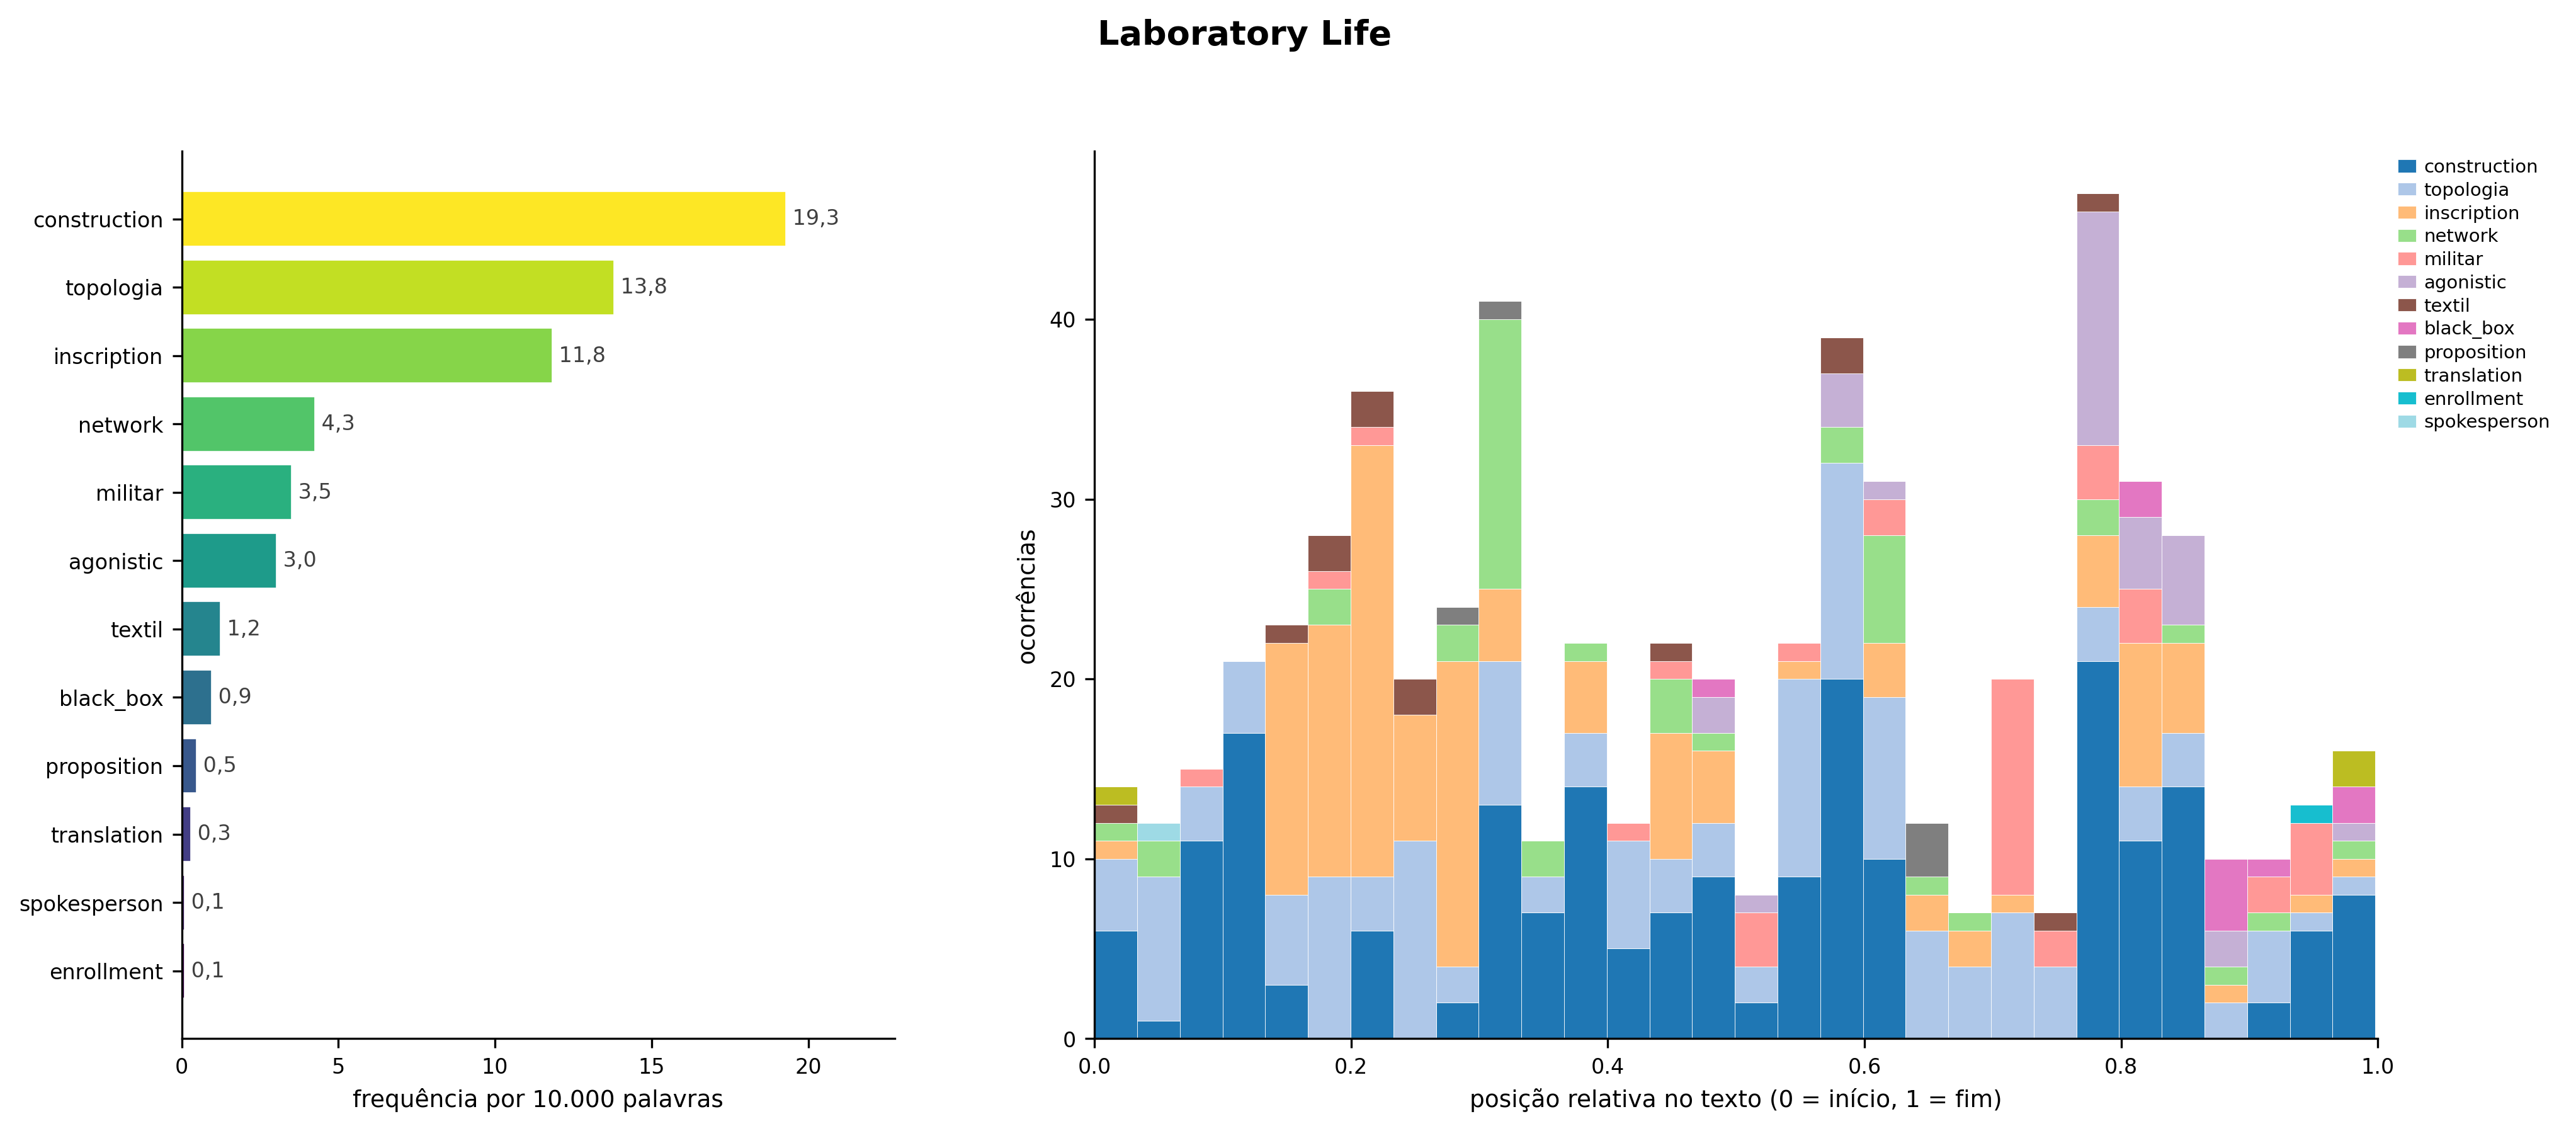
\includegraphics[width=1.0\linewidth]{figuras/cap.2/lexicometria/etapa1_lab_life_freq_e_densidade.png}
\caption[Frequência e distribuição dos rótulos em \emph{Laboratory Life}]{Rótulos do catálogo lexical em \emph{Laboratory Life} (Latour e Woolgar, 1986). À esquerda, a frequência de cada rótulo em ocorrências por dez mil palavras, com o rótulo \texttt{militar} na contagem refinada pela desambiguação de \textit{war}/\textit{wars}; à direita, a distribuição das ocorrências de cada rótulo ao longo do texto, da abertura ao fecho da obra. O vocabulário do construtivismo social, \textit{construction} e \textit{inscription}, domina a frequência, e o rótulo \texttt{militar} aparece em registro contido, coerente com o uso instrumental da analogia militar nesta obra. Fonte: análise das figurações em \url{github.com/julianehelanski/analise-figuracoes-latour}.}
\label{fig:freq_densidade_lab_life}
\end{figure}

% [FIGURA 2] — Science in Action: frequência + densidade.
% Arquivo a regenerar: freq_densidade_sia.png (militar refinado, n=363).
\begin{figure}[htbp]
\centering
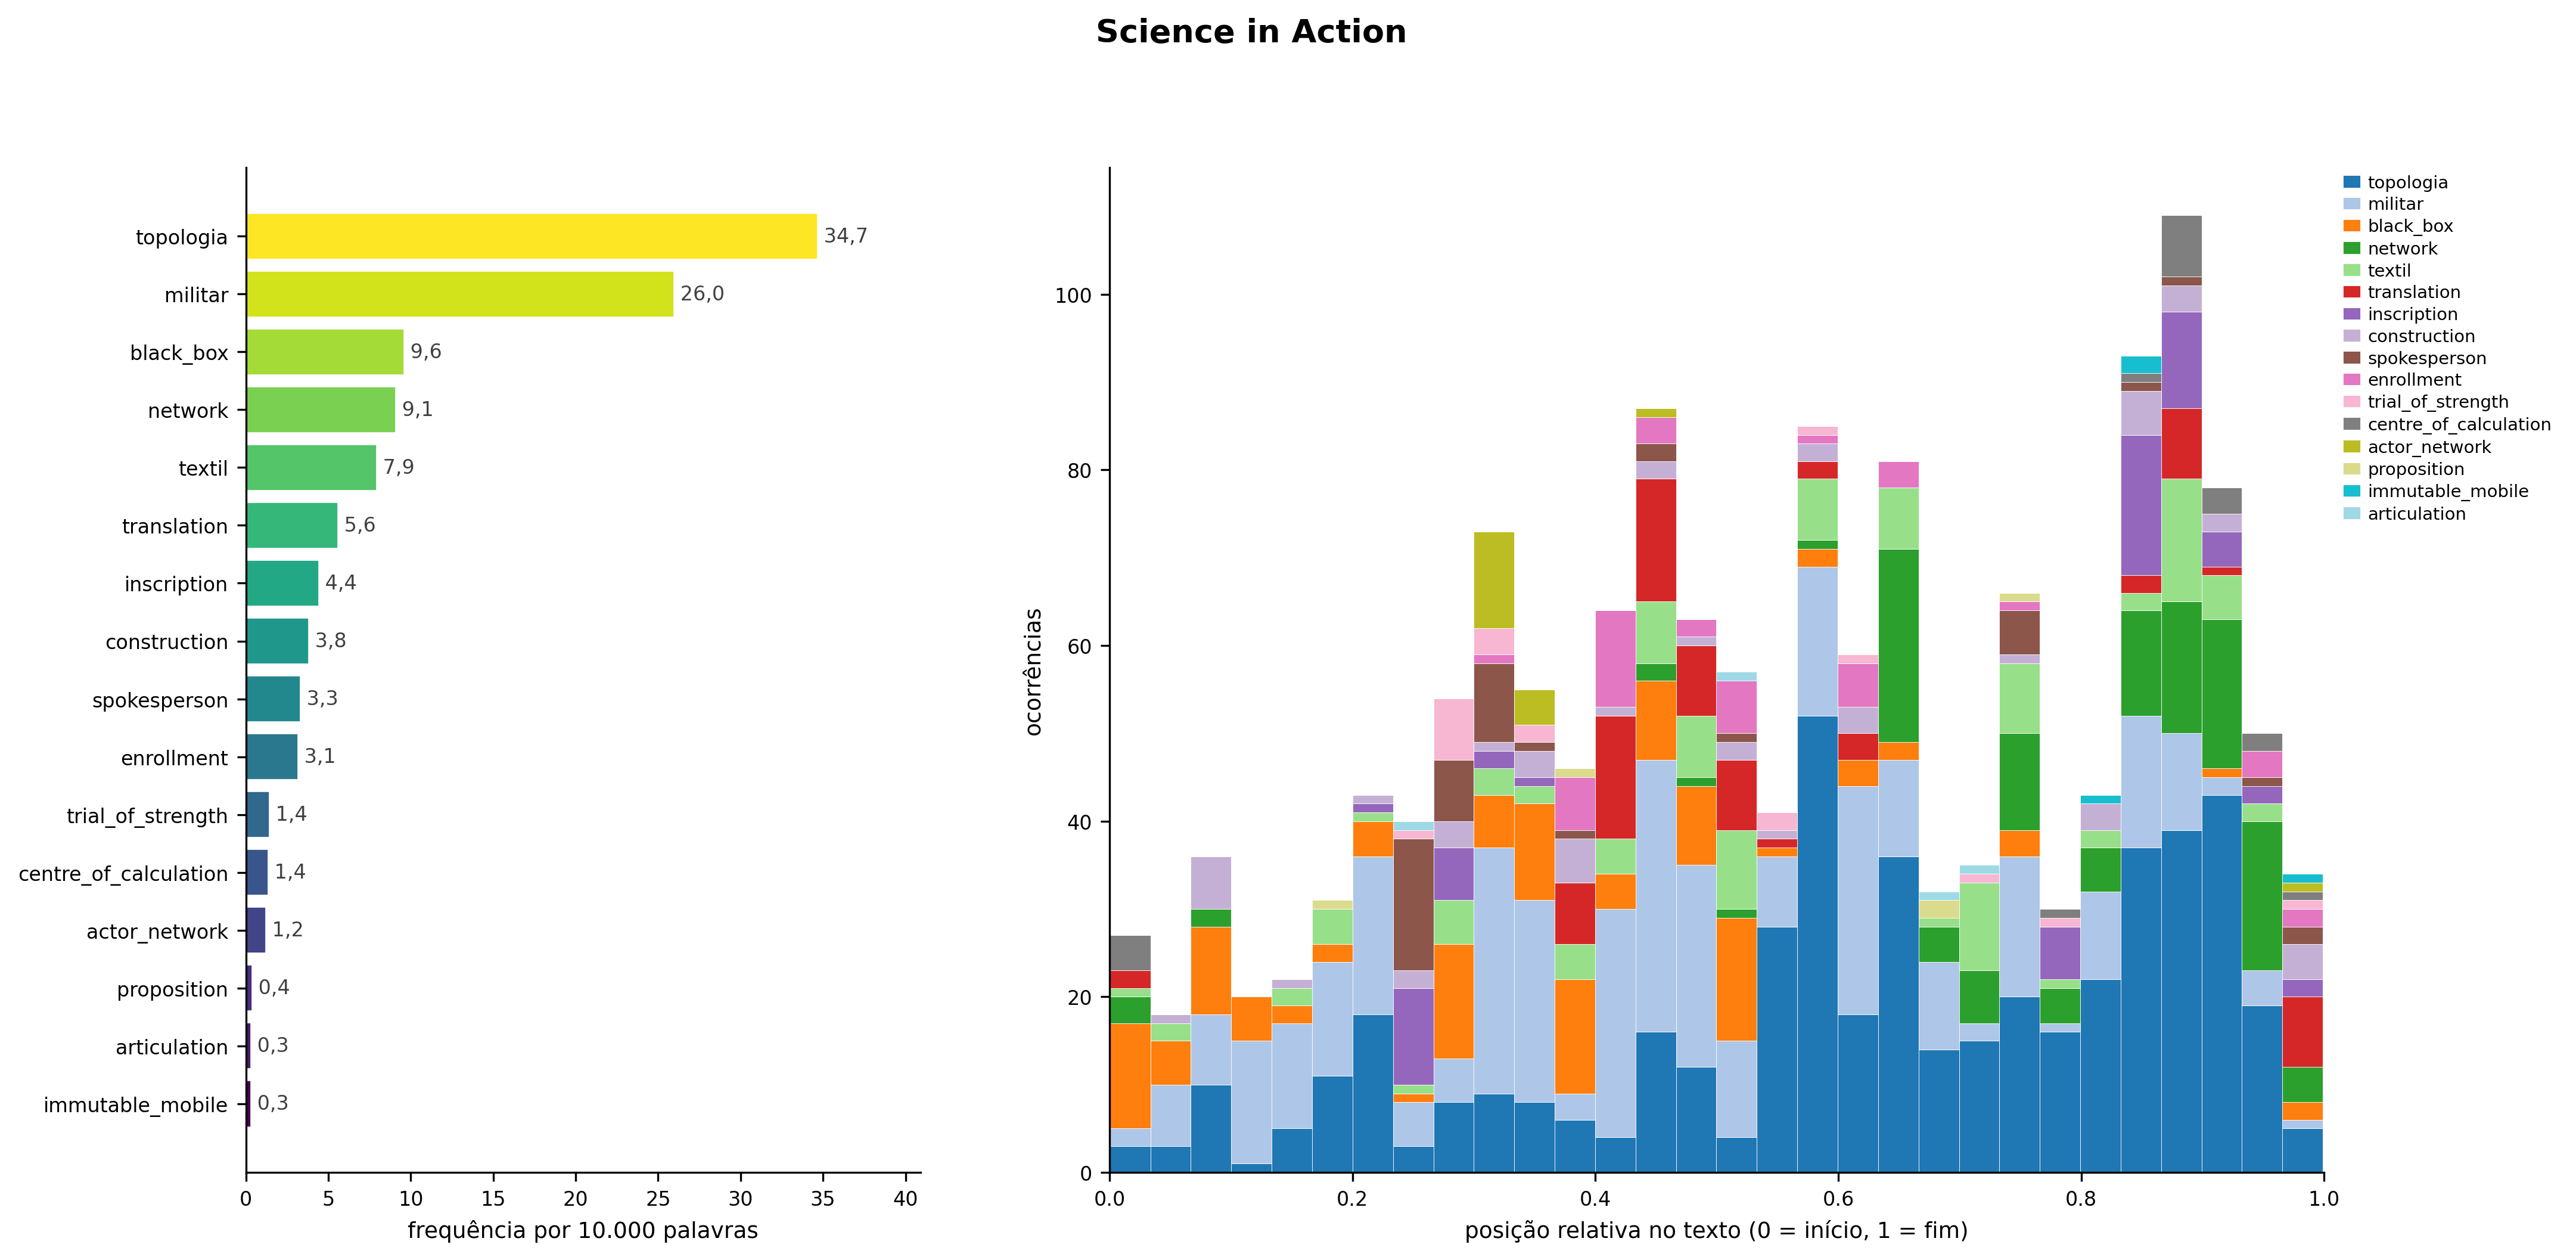
\includegraphics[width=1.0\linewidth]{figuras/cap.2/lexicometria/etapa1_sia_freq_e_densidade.png}
\caption[Frequência e distribuição dos rótulos em \emph{Science in Action}]{Rótulos do catálogo lexical em \emph{Science in Action} (Latour, 1987). À esquerda, a frequência de cada rótulo em ocorrências por dez mil palavras, com o rótulo \texttt{militar} na contagem refinada; à direita, a distribuição das ocorrências ao longo do texto. O rótulo \texttt{militar} encabeça a frequência ao lado de \texttt{topologia}, e a distribuição mostra o vocabulário militar espalhado por toda a extensão da obra. Fonte: análise das figurações em \url{github.com/julianehelanski/analise-figuracoes-latour}.}
\label{fig:freq_densidade_sia}
\end{figure}

% [FIGURA 3] — Pandora's Hope: frequência + densidade.
% Arquivo a regenerar: freq_densidade_pandora.png (militar refinado, n=156).
\begin{figure}[htbp]
\centering
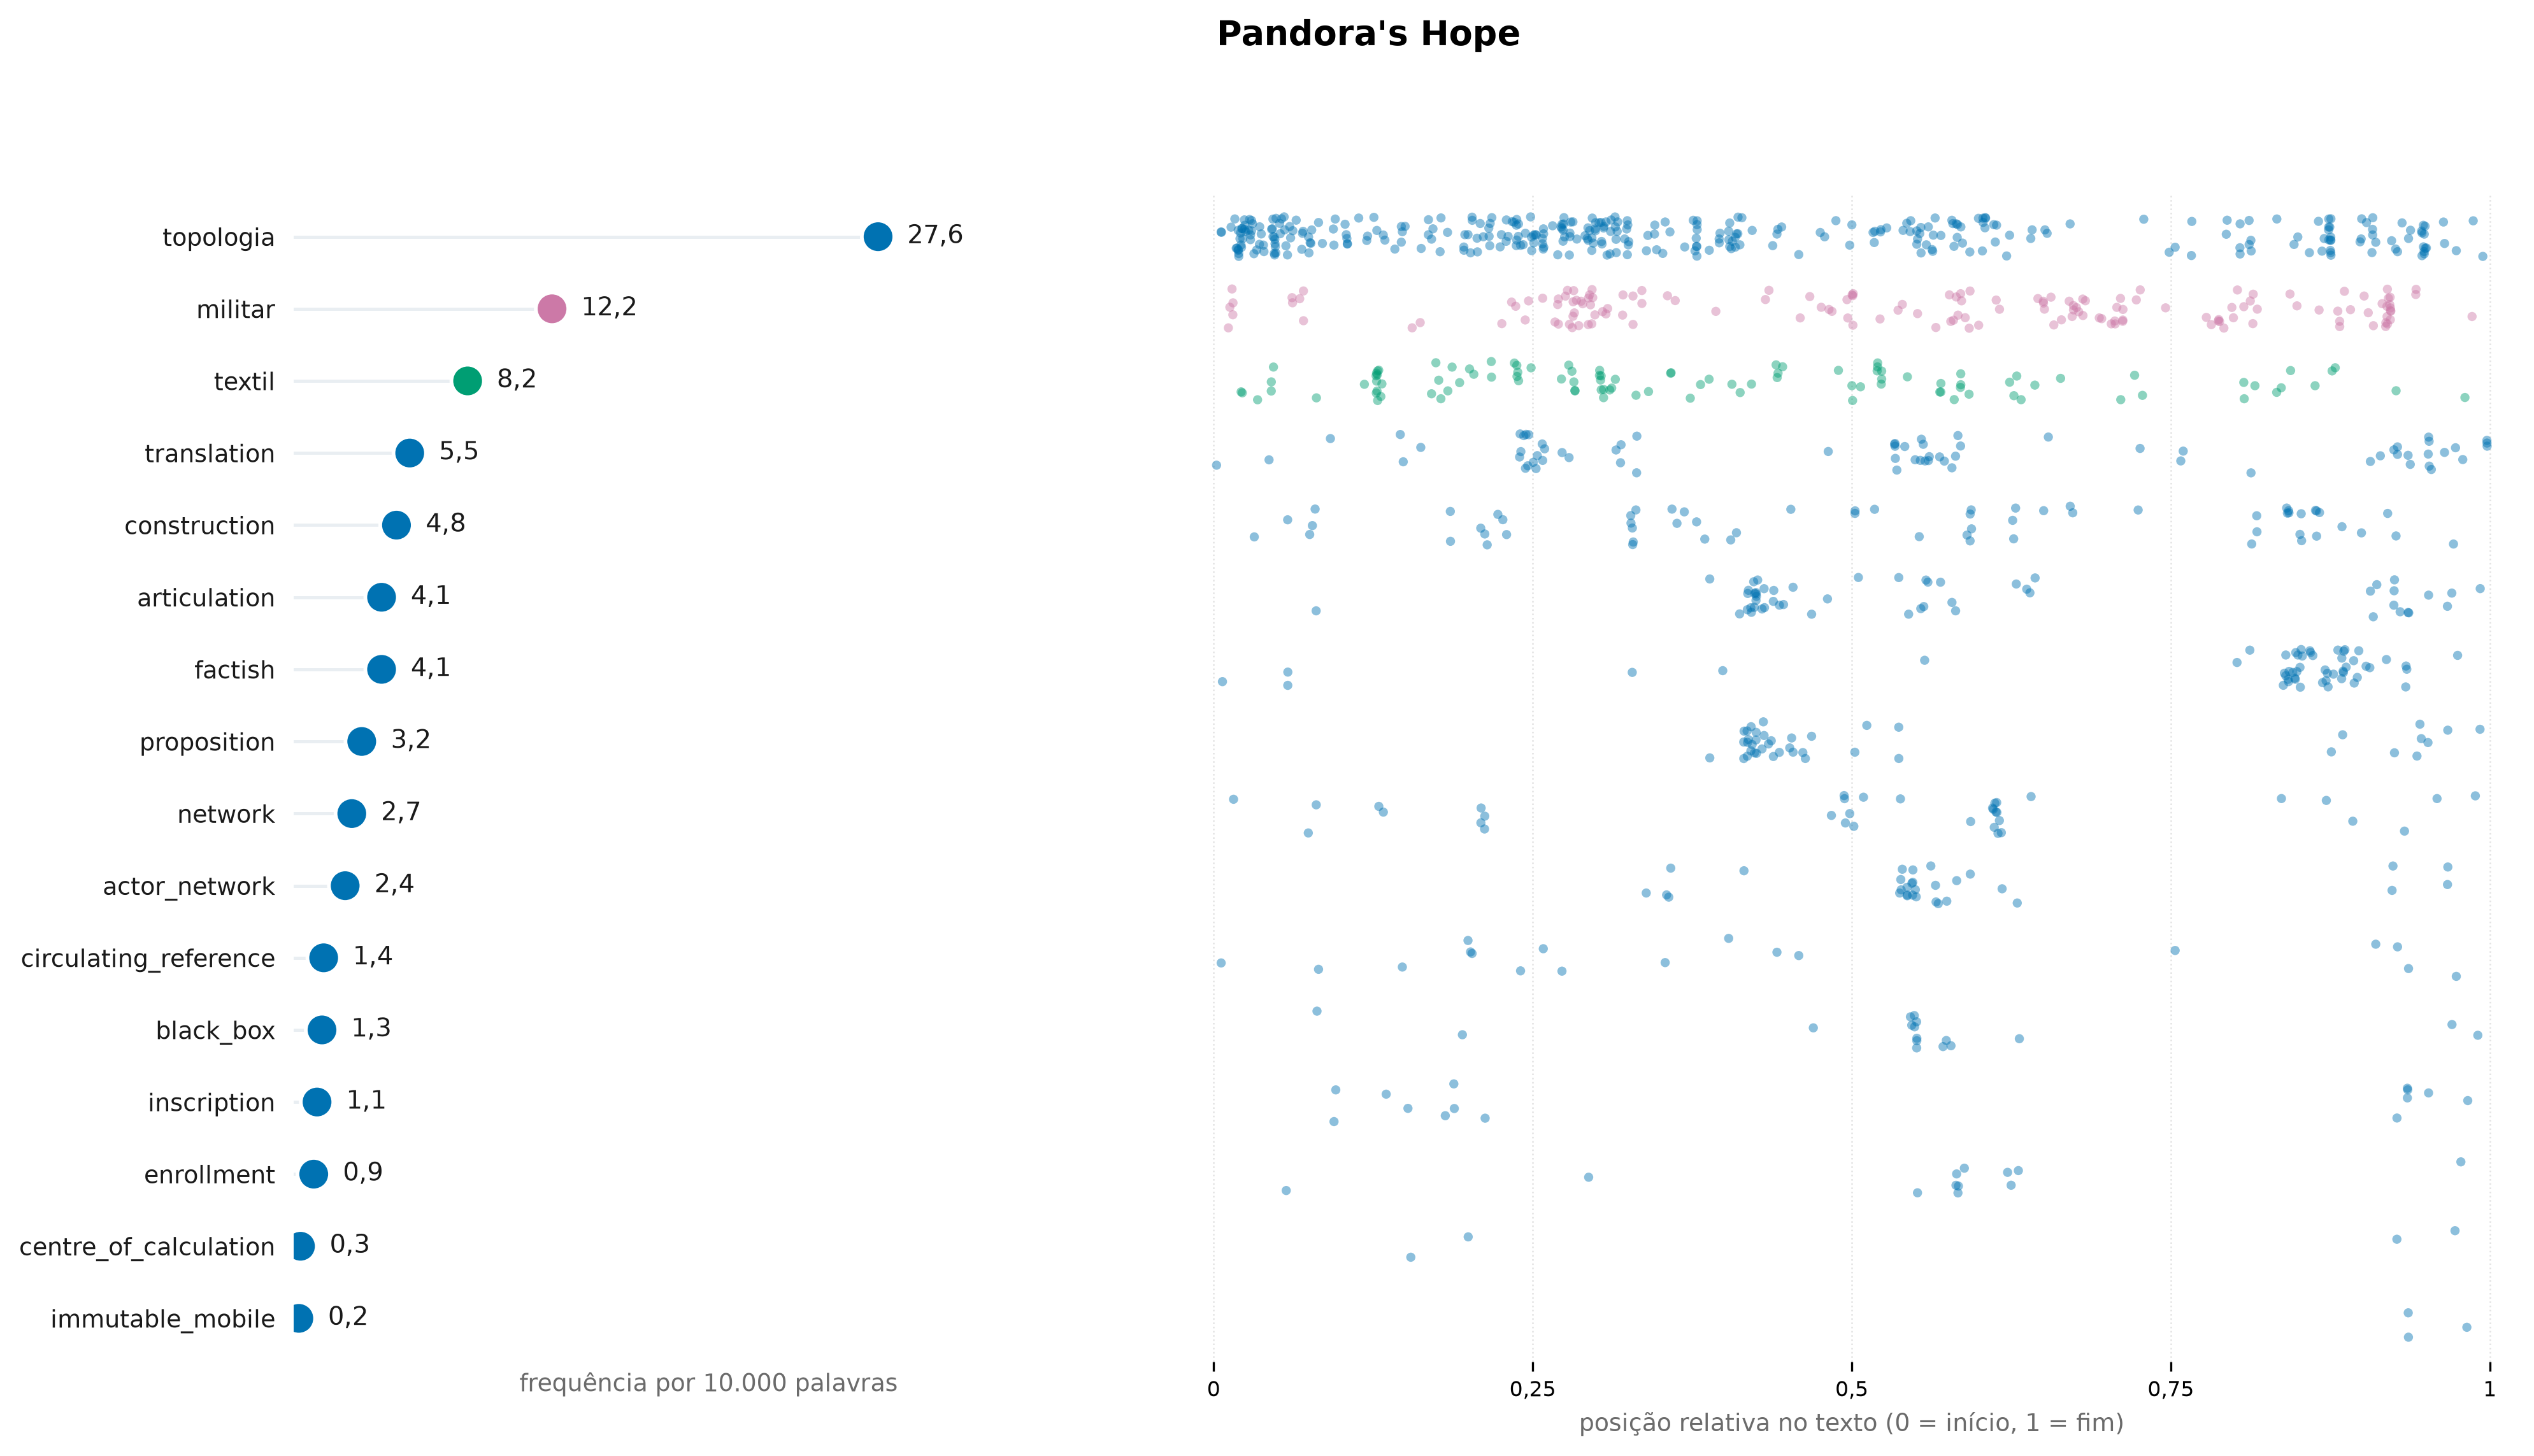
\includegraphics[width=1.0\linewidth]{figuras/cap.2/lexicometria/etapa1_pandora_freq_e_densidade.png}
\caption[Frequência e distribuição dos rótulos em \emph{Pandora's Hope}]{Rótulos do catálogo lexical em \emph{Pandora's Hope} (Latour, 1999). À esquerda, a frequência de cada rótulo em ocorrências por dez mil palavras, com o rótulo \texttt{militar} na contagem refinada; à direita, a distribuição das ocorrências ao longo do texto. O rótulo \texttt{militar} mantém-se em registro alto treze anos depois de \emph{Science in Action}, e a distribuição mostra o vocabulário militar concentrado em picos isolados, em especial na faixa do capítulo sobre Frédéric Joliot e na do epílogo, em contraste com a distribuição contínua de 1987. Fonte: análise das figurações em \url{github.com/julianehelanski/analise-figuracoes-latour}.}
\label{fig:freq_densidade_pandora}
\end{figure}

% [NOTA DE REVISÃO 8] Parágrafo de leitura das figuras por obra.
% Antes este parágrafo lia uma única figura comparativa e remetia a
% uma tabela e a uma segunda figura, ambas removidas. Reescrito para
% ler as três figuras compostas por obra. Os números essenciais
% (3,50 / 25,95 / 12,19 e a substituição agonistic->trial_of_strength)
% sobrevivem no corpo. Regra 4: sem "não X mas Y".
As Figuras~\ref{fig:freq_densidade_lab_life}, \ref{fig:freq_densidade_sia} e~\ref{fig:freq_densidade_pandora} apresentam, obra a obra, a frequência de cada rótulo ao lado da distribuição das ocorrências ao longo do texto. A leitura conjunta das três sustenta dois achados. O primeiro é a magnitude do salto entre \emph{Laboratory Life} e \emph{Science in Action}. Em \emph{Laboratory Life}, escrito com Woolgar, a densidade do rótulo \texttt{militar} fica em 3,50 ocorrências por dez mil palavras, e o vocabulário que domina a obra é o do construtivismo social, \textit{construction} e \textit{inscription};\footnote{O rótulo \texttt{topologia}, que acrescentei ao catálogo na etapa~2 e que apresento adiante, registra em \emph{Laboratory Life} densidade de 13,81 ocorrências por dez mil palavras, valor que o situa entre os rótulos de maior densidade da obra, acima de \textit{inscription}. As Figuras~\ref{fig:freq_densidade_lab_life} a~\ref{fig:freq_densidade_pandora} foram mantidas com os dezessete rótulos da etapa~1 e por isso não exibem o rótulo \texttt{topologia}; a sua densidade nas três obras monográficas consta da contagem do catálogo estendido que apresento na seção seguinte.} em \emph{Science in Action}, escrito por Latour um ano depois, a densidade do rótulo \texttt{militar} salta para 25,95 por dez mil, um aumento de mais de sete vezes, e a figuração militar passa a encabeçar a frequência da obra. O segundo achado é a manutenção da densidade militar em registro alto em \emph{Pandora's Hope}, treze anos depois: 12,19 por dez mil palavras na contagem refinada, ainda mais de três vezes a densidade de \emph{Laboratory Life}. A figuração militar-industrial que se cristaliza em \emph{Science in Action} permanece em registro alto quando Latour, em \emph{Pandora's Hope}, tenta reformular o estatuto ontológico dos fatos científicos pelas noções de \textit{factish} e \textit{circulating reference}. A coluna de distribuição das três figuras acrescenta uma leitura que a frequência sozinha não devolve: no primeiro dos dois livros solo o vocabulário militar se espalha por toda a extensão do texto, ao passo que no segundo ele se concentra em picos isolados, em especial na faixa do capítulo sobre Frédéric Joliot e a fabricação do reator de Ivry às vésperas da Segunda Guerra Mundial e na do epílogo. O contraste entre as duas distribuições sustenta a leitura de que, em \emph{Science in Action}, a figuração militar funciona como prosa argumentativa, e que, em \emph{Pandora's Hope}, ele se concentra em momentos específicos no argumento. O KWIC, \textit{keyword in context}, confirma o registro descritivo de \emph{Science in Action}: os termos que dominam a contagem aparecem sem aspas distanciadoras, como em \enquote{technoscience is part of a war machine and should be studied as such} \parencite[p.~192]{Latour1987Science}.\footnote{Tradução brasileira: \textcite{Latour2011CienciaEmAcao}, p.~\texttt{[p. 269]}.} As três figuras compostas têm escalas de frequência independentes, próprias a cada obra, e por isso a comparação direta de magnitude entre elas pede uma quarta figura. A Figura~\ref{fig:comparacao_tres_obras} põe as três obras na mesma escala de densidade e torna o salto imediatamente legível: o rótulo \texttt{militar} passa de 3,50 ocorrências por dez mil palavras em 1986 a 25,95 em 1987, e se mantém em 12,19 em 1999.

A densidade dos rótulos surgem do encontro entre três coisas: das obras que Latour escreveu, do catálogo de rótulos que eu construí e da janela de contexto que defini para contar as ocorrências. Um catálogo com mais rótulos e mais termos por rótulo registra mais ocorrências e mais co-ocorrências (proximidade textual), e uma janela mais ampla aproxima mais termos; a densidade que vejo na figura responde a essas escolhas tanto quanto responde à escrita de Latour. Isso não retira valor à medida, e tampouco a relativiza ao ponto de torná-la arbitrária: significa que a densidade só sustenta o argumento quando eu a leio de modo situado, na comparação entre obras analisadas sob o mesmo catálogo e a mesma janela, e quando declaro o instrumento com que a produzi. É por essa razão que mantenho o catálogo e a janela constantes nas cinco obras das etapas~1 e~2, e que apresento as figuras obra a obra antes de qualquer comparação agregada, isso significa que a comparabilidade é uma das condição que eu construo. Tomada assim, a variação de densidade entre as obras deixa de ser um número a constatar e passa a delinear a variedade de registros figurativos com que Latour descreveu a tecnociência e a teoria ao longo dessa seis obras e aqui as interpreto como uma trajetória intelectual. 

A cristalização do léxico militar em \emph{Science in Action} acompanha-se da substituição interna ao catálogo que descrevi acima. O termo \textit{agonistic}, que em \emph{Laboratory Life} aparece trinta e duas vezes e descreve o campo em que enunciados são testados, desaparece completamente em \emph{Science in Action} e em \emph{Pandora's Hope}. Em outra direção, \textit{trial of strength} surge pela primeira vez em \emph{Science in Action}, com vinte ocorrências, e descreve um gesto semelhante ao do agon: \enquote{trials of strength to evaluate the resistance of the ties that link the representatives to what they speak for} \parencite[p.~93]{Latour1987Science}.\footnote{Tradução brasileira: \textcite{Latour2011CienciaEmAcao}, p.~\texttt{[p. 118]}.} A substituição, do agon ao julgamento de força, marca um deslocamento do registro pragmático-filosófico, em que o agon nomeia o jogo da prova com um vocabulário herdado da retórica clássica, para um registro topológico-militar, em que a prova é medida por resistências, laços e mobilizações. O agon perde o estatuto de figura organizadora, e o vocabulário militar passa a ocupar o seu lugar com uma densidade que, como mostra a figura~\ref{fig:freq_densidade_sia}, é a marca distintiva de \emph{Science in Action} no conjunto do corpus.\footnote{A desambiguação de \textit{war}/\textit{wars} descrita acima incide de modo desigual sobre as três obras, e é esse efeito desigual que sustenta o seu uso: a queda do rótulo \texttt{militar} é de 26,4\% em \emph{Pandora's Hope}, ao passo que em \emph{Science in Action} é de 2,9\% e em \emph{Laboratory Life} de 5,1\%. O pico de \emph{Science in Action} permanece, assim, como ponto de cristalização da figuração militar-industrial em registro figurativo mesmo depois de descontado o uso histórico de \textit{war}.}

A morfologia da distribuição do léxico militar ao longo dos textos, visível nos painéis de densidade das figuras~\ref{fig:freq_densidade_sia} e~\ref{fig:freq_densidade_pandora}, sustenta uma leitura adicional sobre o estatuto que o rótulo \texttt{militar} ocupa em cada obra. Em \emph{Science in Action}, a distribuição é contínua e relativamente homogênea, com vários picos médios distribuídos por praticamente toda a extensão do texto: o vocabulário militar não está confinado a uma seção ou capítulo, atravessa transversalmente a obra e funciona de forma recorrente à prosa argumentativa. Em \emph{Pandora's Hope}, a distribuição apresenta picos mais altos e isolados, separados por trechos longos de densidade baixa ou nula, e os picos correspondem em sua maioria ao capítulo sobre a trajetória de Frédéric Joliot e a fabricação do reator de Ivry e ao epílogo da obra. Essa distribuição sustenta a leitura de que, em \emph{Pandora's Hope}, o vocabulário militar se concentra em momentos argumentativamente situados, enquanto em \emph{Science in Action} ele se distribui em camadas descritivas contínuas das práticas tecnocientíficas.

A contagem de co-ocorrências completa essa leitura. Calculei a co-ocorrência entre os rótulos do catálogo em janelas de duzentas palavras, sobre o texto integral de \emph{Science in Action}, e o resultado é uma matriz que cruza cada rótulo com todos os demais.\footnote{A matriz de co-ocorrência conta o rótulo \texttt{militar} na contagem bruta, e não na refinada pela desambiguação de \textit{war}/\textit{wars} que adoto no restante deste capítulo~\ref{capitulo2}. O cálculo da co-ocorrência incide sobre o arquivo de \textit{keyword in context} antes do refinamento, e refinar a matriz exigiria reprocessar a co-ocorrência sobre um KWIC já refinado. Registro a opção como limitação conhecida, documentada no repositório, e observo que ela não desloca a ordem de grandeza nem a hierarquia dos pares que reporto.} A leitura dessa matriz mostra um ponto que a contagem agregada, rótulo a rótulo, não devolve. O par mais denso de toda a rede de co-ocorrência de \emph{Science in Action} é \texttt{militar}--\texttt{topologia}, com quatrocentas e noventa e cinco co-ocorrências, valor que supera em mais de três vezes o do par \texttt{militar}--\textit{black box}. O vocabulário militar e o vocabulário topológico, que esta tese reconhece, ao lado do têxtil, como o polo que tensiona a figuração militar-industrial, já aparecem entrelaçados em \emph{Science in Action}, na obra de 1987, antes dos artigos metateóricos em que Latour passa a refletir sobre a sua própria teoria. A densidade desse entrelaçamento não é um caso isolado na matriz, os três pares mais densos depois de \texttt{militar}--\texttt{topologia} são \texttt{network}--\texttt{topologia}, com trezentas e sessenta co-ocorrências, \texttt{textil}--\texttt{topologia}, com cento e sessenta e seis, e \texttt{militar}--\texttt{textil}, com cento e cinquenta e cinco, e os quatro pares reúnem o vocabulário militar, o topológico e o têxtil já na obra que cristaliza a figuração militar-industrial. O vocabulário militar aparece, ainda, em vizinhança dos conceitos pelos quais a teoria ator-rede foi recebida como descrição da prática científica: na mesma janela de duzentas palavras, o rótulo \texttt{militar} co-ocorre cento e cinquenta e duas vezes com \textit{black box}, noventa e oito com \textit{network}, setenta e duas com \textit{inscription} e setenta e uma com \textit{translation}, além de cinquenta e nove vezes com \textit{construction}, cinquenta e cinco com \textit{spokesperson} e cinquenta e duas com \textit{enrollment}. Os termos pelos quais a teoria circulou como descrição neutra, \textit{black box}, \textit{network}, \textit{translation} e \textit{inscription}, aparecem, no texto de 1987, na vizinhança recorrente tanto do vocabulário militar quanto do vocabulário topológico. A matriz de co-ocorrência completa, rótulo a rótulo, fica versionada no repositório.

\begin{figure}[htbp]
\centering
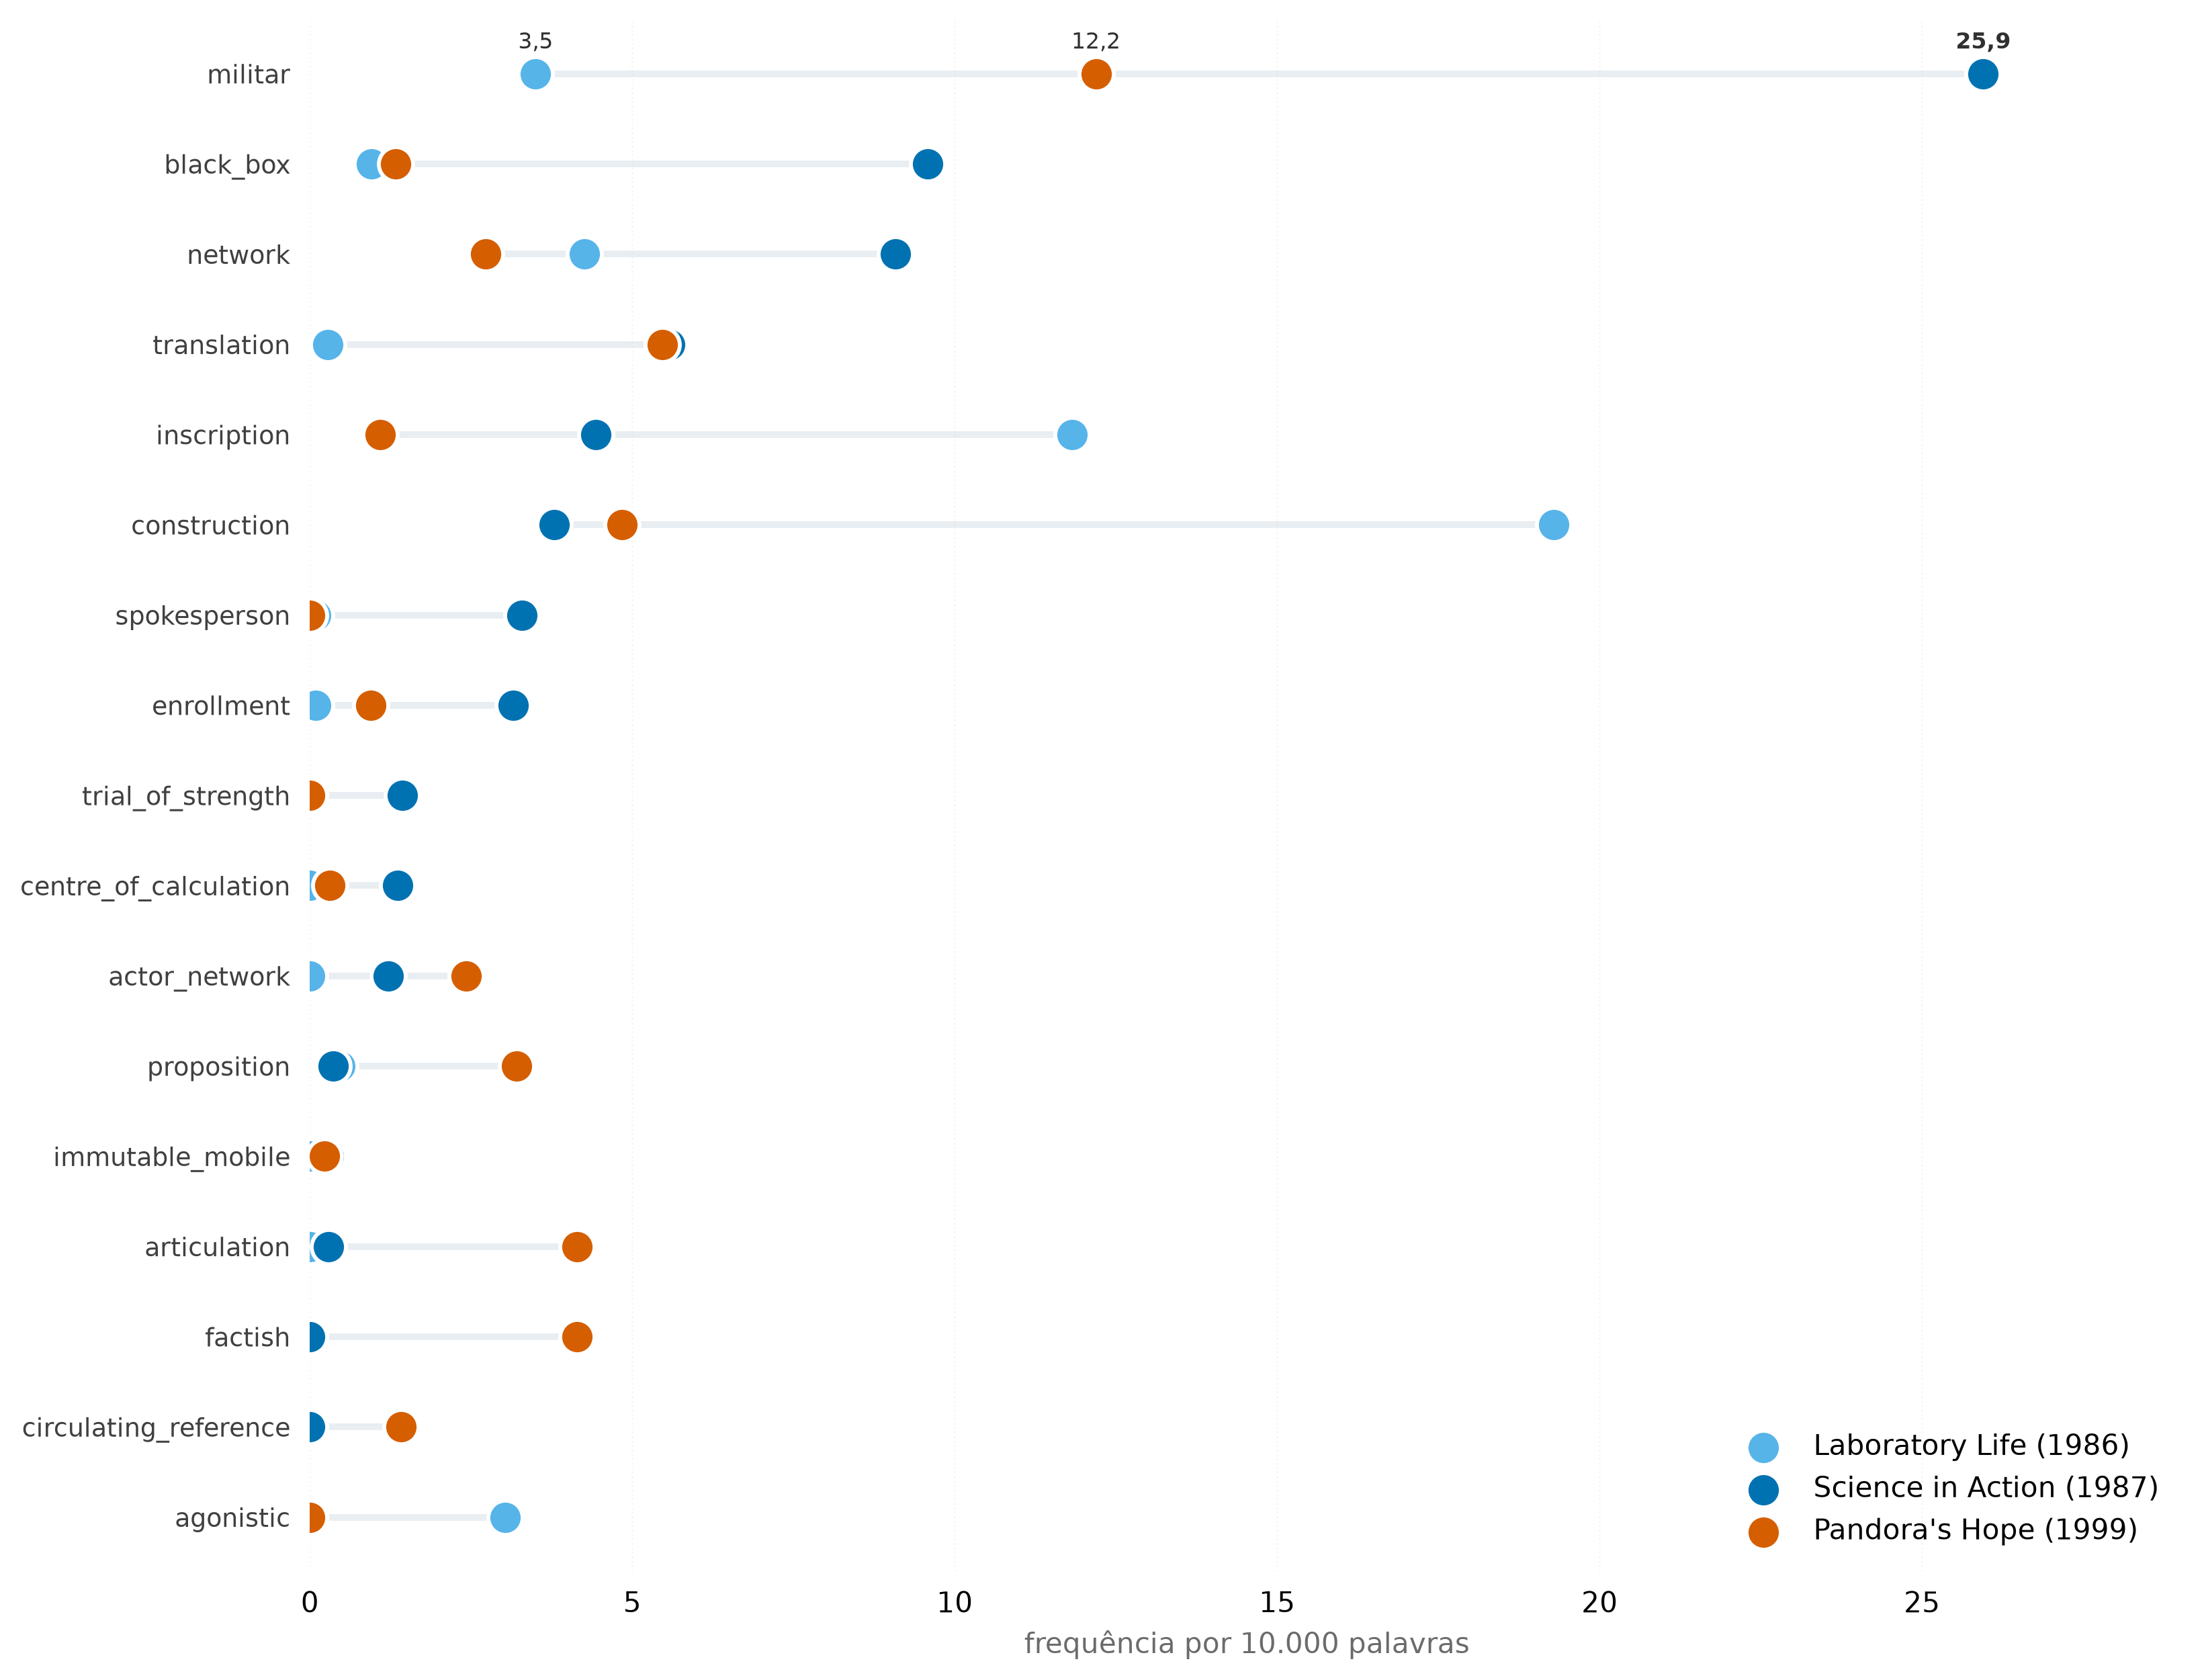
\includegraphics[width=0.85\linewidth]{figuras/cap.2/lexicometria/etapa1_passo4_comparacao_frequencias_tres_obras.png}
\caption[Densidade comparada dos rótulos nas três obras de Latour]{Densidade dos dezessete rótulos do catálogo lexical nas três obras de Latour em escopo da etapa~1, \emph{Laboratory Life} (1986), \emph{Science in Action} (1987) e \emph{Pandora's Hope} (1999), em ocorrências por dez mil palavras e em escala comum às três obras. Cada rótulo é uma linha, e os três pontos ligados pela linha-guia correspondem às três obras em ordem cronológica de publicação, \emph{Laboratory Life} em azul claro, \emph{Science in Action} em azul e \emph{Pandora's Hope} em vermelho. O rótulo \texttt{militar} aparece no topo, com a maior amplitude entre as três obras, na contagem refinada pela desambiguação simétrica de \textit{war}/\textit{wars}, com os valores 3,50 em 1986, 25,95 em 1987 e 12,19 em 1999 anotados acima dos seus pontos. A escala comum às três obras torna legível o salto na densidade do rótulo \texttt{militar} entre 1986 e 1987 e a sua manutenção em registro alto em 1999. Fonte: análise das figurações em \url{github.com/julianehelanski/analise-figuracoes-latour}.}
\label{fig:comparacao_tres_obras}
\end{figure}

A etapa~1 alcançou os dezessete rótulos do catálogo, e o relatório completo, com a matriz cruzada e os rankings por obra individual, fica disponível no repositório.\footnote{O relatório consolidado e a matriz cruzada completa dos dezessete rótulos por obra estão em \url{github.com/julianehelanski/analise-figuracoes-latour}, na pasta de \emph{outputs}. Os rankings de frequência interna, os mapas de densidade ao longo do texto e as redes de co-ocorrência calculados obra a obra ficam nas subpastas de cada obra.} O que retenho aqui da etapa~1 é o que dá nome ao ponto sensível da escrita latouriana: a figuração militar-industrial que descrevi por leitura de passagens escolhidas aparece como resultado contável da escrita que Latour produziu em \emph{Science in Action} e manteve, em densidade atenuada e ainda dominante, em \emph{Pandora's Hope}. A análise corroborou a leitura qualitativa que eu sustentava por amostras, e ofereceu medida sistemática da magnitude do deslocamento de \emph{Laboratory Life} a \emph{Pandora's Hope}, em forma auditável.

% =====================================================================
% ETAPA 2 e ETAPA 2-bis
% =====================================================================
\subsection{O corpus estendido: o vocabulário metateórico de \emph{Clarifications} e \emph{On Recalling ANT}}
\label{subsubsec:trajetoria_estendida_metateorica}

A análise sobre as três obras da etapa 1 faz parte de um trabalho maior, que estendi com a inclusão de dois artigos nos quais Latour propõe uma nova interpretação sobre a teoria ator-rede. A inclusão desses dois artigos vieram de uma leitura anterior em que observei um contraste de posicionamento e conceitual de Latour diferente dos livros. Se o vocabulário militar-industrial é um dos pontos sensíveis da obra de Latour, e o é sobretudo quando passa a explicar a prática tecnocientífica, então é razoável esperar que esse vocabulário se reorganize quando Latour, de modo autorreflexivo, reinterpreta a própria teoria que vinha desenvolvendo. Os dois artigos metateóricos que escolhi para essa etapa da análise, \emph{On Actor-Network Theory: A Few Clarifications}, de 1996 \parencite{latour1996clarifications}, e \emph{On Recalling ANT}, de 1999 \parencite{Latour1999RecallingANT}, são textos curtos em comparação com os três livros, e Latour os escreveu para esclarecer, defender e reformular a teoria ator-rede diante de seus críticos.\footnote{A análise de \emph{On Recalling ANT} incide sobre o texto integral do artigo.} Os dois artigos não descrevem laboratórios, controvérsias ou alianças sociotécnicas, descrevem a teoria que descreve essas coisas. Essa diferença é o ponto de partida da segunda etapa da análise: o que acontece com a densidade dos rótulos quando o objeto da descrição passa de \emph{tecnociência em ação} para \emph{teoria da tecnociência em ação}?

A leitura qualitativa dos dois artigos, anterior à análise lexicométrica, mostrou que eles empregam um vocabulário têxtil-topológico em densidade que os três livros não haviam apresentado, e que o catálogo original não dispunha de rótulo lexical capaz de captar esse vocabulário. Por isso, e em consequência do gesto reflexivo que organiza este capítulo~\ref{capitulo2}, ampliei o catálogo de dezessete para dezenove rótulos, com o acréscimo dos rótulos \texttt{textil} e \texttt{topologia}, sobretudo a partir de \emph{On Actor-Network Theory: A Few Clarifications}.\footnote{Os termos do rótulo \texttt{textil}, entre eles \textit{fabric}, \textit{thread}, \textit{wire}, \textit{string}, \textit{rope}, \textit{capillary}, \textit{fibrous}, \textit{thread-like}, \textit{wiry}, \textit{stringy} e \textit{ropy}, e os termos do rótulo \texttt{topologia}, entre eles \textit{topology}, \textit{node}, \textit{connection}, \textit{flat}, \textit{folded}, \textit{outside}, \textit{circulating}, \textit{flow} e \textit{scale}, foram catalogados a partir de duas passagens-chave: a definição da teoria ator-rede como mudança de topologia em \emph{Clarifications} e a formulação da topologia como \emph{flat and folded} em \emph{On Recalling ANT}. Apliquei o acréscimo simetricamente sobre as cinco obras, e mantive as figuras da etapa~1 com os dezessete rótulos originais, para preservar a coerência da leitura cronológica nas três primeiras obras.} A análise lexicométrica sobre o corpus estendido sustenta três achados que reorganizam a interpretação dos dados dos três livros iniciais. O primeiro achado é a queda do rótulo \texttt{militar} nos dois textos metateóricos: a densidade bruta do rótulo \texttt{militar} cai de 26,74 por dez mil palavras em \emph{Science in Action} para 3,82 em \emph{Clarifications}, valor próximo do que se observa em \emph{Laboratory Life}, de 3,69.\footnote{Adoto a contagem bruta nesta comparação entre as obras porque a desambiguação de \textit{war}/\textit{wars} foi aplicada aos três livros, e a contagem bruta é a base comum que permite comparar as cinco sem assimetria de procedimento. A diferença entre bruta e refinada não altera a ordem de grandeza da queda aqui descrita. \emph{Laboratory Life} é o único dos três livros escrito em coautoria, com Steve Woolgar, e a coincidência entre sua densidade militar e a dos dois artigos metateóricos sugere que a inflexão militar-industrial se consolida com Latour autor solo em \textit{Science in Action}. Todavia, esse dado é insuficiente para sustentar qualquer generalização sobre o efeito da coautoria.} No corpus integral do \emph{Recalling}, a densidade bruta do rótulo \texttt{militar} é de 4,15 por dez mil palavras, correspondente a duas ocorrências, uma descritivo-histórica, \emph{Science Wars}, e uma metalinguística, \emph{alliance} na lista canônica do vocabulário da teoria ator-rede. O segundo achado é a magnitude dos rótulos \texttt{topologia} e \texttt{textil} nos dois artigos: a densidade de \texttt{topologia} salta de 34,68 por dez mil palavras em \emph{Science in Action} para 150,36 em \emph{Clarifications} e 99,48 no \emph{Recalling} integral, três a quatro vezes a densidade observada nos três livros; a densidade de \texttt{textil} salta de 7,94 em \emph{Science in Action} e 8,20 em \emph{Pandora's Hope} para 49,69 em \emph{Clarifications}, mais de seis vezes a densidade média nos três livros. O terceiro achado é a dominância do rótulo \texttt{network} nos dois artigos: 118,50 por dez mil palavras em \emph{Clarifications} e 58,03 no \emph{Recalling} integral, contra 9,08 em \emph{Science in Action} e 2,73 em \emph{Pandora's Hope}.

\begin{longtable}{@{}p{0.23\textwidth} p{0.20\textwidth} p{0.49\textwidth}@{}}
\caption[Catálogo lexical das etapas 1 e 2]{Catálogo lexical das etapas 1 e 2: os dezenove rótulos rastreados nas obras de Latour, com a procedência de cada rótulo e uma amostra dos termos que o definem. A amostra segue a ordem do arquivo de definição: rótulos com até oito termos aparecem completos, rótulos maiores trazem os oito primeiros termos seguidos de \enquote{entre outros}. A lista completa de termos está no repositório, em \url{github.com/julianehelanski/analise_figuracoes/tree/main/campos_lexicais}.}\label{tab:catalogo-etapas12}\\
\toprule
Campo & Procedência & Amostra de termos do catálogo \\
\midrule
\endfirsthead
\caption[]{Catálogo lexical das etapa s 1 e 2 (continuação).}\\
\toprule
Campo & Procedência & Amostra de termos do catálogo \\
\midrule
\endhead
\midrule
\multicolumn{3}{r@{}}{\footnotesize continua na próxima página}\\
\endfoot
\bottomrule
\endlastfoot
\texttt{inscription} & conceito de Latour & \texttt{inscription}, \texttt{inscriptions}, \texttt{inscription device}, \texttt{inscription devices}, \texttt{literary inscription} \\
\texttt{immutable\_mobile} & conceito de Latour & \texttt{immutable mobile}, \texttt{immutable mobiles} \\
\texttt{black\_box} & conceito de Latour & \texttt{black box}, \texttt{black-box}, \texttt{black boxes}, \texttt{blackbox}, \texttt{blackboxing}, \texttt{black-boxing} \\
\texttt{centre\_of\_calculation} & conceito de Latour & \texttt{centre of calculation}, \texttt{center of calculation}, \texttt{centres of calculation}, \texttt{centers of calculation} \\
\texttt{actor\_network} & conceito de Latour & \texttt{actor-network}, \texttt{actor network}, \texttt{actant}, \texttt{actants} \\
\texttt{translation} & conceito de Latour & \texttt{translation}, \texttt{translations}, \texttt{translate}, \texttt{translates}, \texttt{translated} \\
\texttt{trial\_of\_strength} & conceito de Latour & \texttt{trial of strength}, \texttt{trials of strength} \\
\texttt{factish} & conceito de Latour & \texttt{factish}, \texttt{factishes} \\
\texttt{circulating\_reference} & conceito de Latour & \texttt{circulating reference}, \texttt{circulating references} \\
\texttt{articulation} & conceito de Latour & \texttt{articulation}, \texttt{articulations}, \texttt{articulate}, \texttt{articulated} \\
\texttt{construction} & conceito de Latour & \texttt{construction}, \texttt{constructed}, \texttt{constructing}, \texttt{social construction} \\
\texttt{proposition} & conceito de Latour & \texttt{proposition}, \texttt{propositions} \\
\texttt{network} & conceito de Latour & \texttt{network}, \texttt{networks}, \texttt{networking} \\
\texttt{agonistic} & conceito de Latour & \texttt{agonistic}, \texttt{agonistics}, \texttt{agonistic field} \\
\texttt{enrollment} & conceito de Latour & \texttt{enrollment}, \texttt{enrolment}, \texttt{enroll}, \texttt{enrol}, \texttt{enrolled} \\
\texttt{spokesperson} & conceito de Latour & \texttt{spokesperson}, \texttt{spokespersons}, \texttt{spokesman}, \texttt{spokesmen}, \texttt{spokeswoman} \\
\texttt{militar} & rótulo reunido & \texttt{ally}, \texttt{allies}, \texttt{allied}, \texttt{alliance}, \texttt{alliances}, \texttt{enemy}, \texttt{enemies}, \texttt{enmity}, entre outros \\
\texttt{textil} & rótulo reunido & \texttt{thread}, \texttt{threads}, \texttt{threading}, \texttt{threaded}, \texttt{thread-like}, \texttt{threadlike}, \texttt{weave}, \texttt{weaves}, entre outros \\
\texttt{topologia} & rótulo reunido & \texttt{fluid}, \texttt{fluids}, \texttt{fluidity}, \texttt{surface}, \texttt{surfaces}, \texttt{node}, \texttt{nodes}, \texttt{connection}, entre outros \\
\end{longtable}

A partir desses três deslocamentos fiz uma desambiguação simétrica à que apliquei ao rótulo \texttt{militar} nos três livros. A análise refinada do rótulo \texttt{militar} nos dois artigos chega a zero em todas as versões do corpus: as três ocorrências em \emph{Clarifications}, \textit{allies}, \textit{enemies} e \textit{alliance}, e as duas ocorrências no \emph{Recalling} integral foram todas classificadas como uso bibliográfico, metalinguístico, descritivo-histórico ou de polêmica conceitual, e nenhuma aparece como tropo figurativo internamente latouriano. \emph{Clarifications} traz \textit{alliance} apenas na referência bibliográfica a \emph{La nouvelle alliance} de Prigogine e Stengers; \textit{allies} aparece em formulação que polemiza com a leitura corrente da teoria ator-rede como rede de aliados homens em luta por poder, formulação que Latour cita para rejeitar e que descreve como \enquote{about as accurate as saying that the night sky is black because the astrophysicists have shown there is a big black hole in it} \parencite[p.~5]{latour1996clarifications}; \textit{enemies} aparece em contexto epistemológico sobre os \enquote{reflexivists} e seus \enquote{pre-relativist enemies}, em registro polêmico que cita posições teóricas adversárias sem mobilizar o vocabulário militar para descrever a prática científica. No \emph{Recalling} integral, a lexicometria incorpora a ocorrência metalinguística de \textit{alliance} que estava ausente do corpus parcial: Latour cita os termos canônicos da teoria ator-rede, \textit{association}, \textit{translation}, \textit{alliance} e \textit{obligatory passage point}, para classificá-los como vocabulário pobre a ser substituído. Das duas únicas ocorrências brutas da figuração militar no \emph{Recalling} integral, nenhuma mobiliza o vocabulário militar como tropo da prática científica. O rótulo \texttt{militar} desaparece, refinado, dos textos em que Latour fala sobre a teoria ator-rede, e permanece concentrado nos textos em que ele a aplica para descrever a tecnociência.

A inversão entre o rótulo \texttt{militar} e os rótulos \texttt{textil} e \texttt{topologia} sustenta, de modo geral, a leitura figurativa que faço da obra latouriana ao longo do tempo. Onde o vocabulário militar predomina, o vocabulário têxtil-topológico permanece em registro subordinado, ao passo que, onde o vocabulário militar se ausenta, é o têxtil-topológico que ocupa o lugar e organiza a descrição. Nos três livros, em que Latour descreve a tecnociência, o rótulo \texttt{militar} alcança densidades de 3,50 a 25,95 por dez mil palavras e o rótulo \texttt{topologia} se mantém entre 13,81 e 34,68. Já nos dois artigos metateóricos, em que Latour descreve a teoria, o rótulo \texttt{militar} cai a zero na contagem refinada e o rótulo \texttt{topologia} sobe a 150,36 em \emph{Clarifications} e a 99,48 no \emph{Recalling} integral. A leitura qualitativa das passagens em que esses rótulos aparecem nos artigos sustenta o achado em registro denotativo. Em \emph{Clarifications}, Latour formula a teoria ator-rede de modo que que condensa o deslocamento do vocabulário militar para o têxtil-topológico: 

\begin{citacaoabnt}
Put too simply AT is a change of methaphors to describe essences: instead of surfaces one gets filaments (or rhyzomes in Deleuze's parlance). More precisely it is a change of topology. Instead of thinking in terms of surfaces, two dimension, or spheres, three dimension, one is asked to think in terms of nodes that have as many dimensions as they have connections. As a first approximation, the AT claims that modern societies cannot be described without recognizing them as having a fibrous, thread-like, wiry, stringy, ropy, capillary character that is never captured by the notions of levels, layers, territories, spheres, categories, structure, systems. \parencite[p.~3]{latour1996clarifications}
\end{citacaoabnt}

% [NOTA DE REVISÃO 17] No original \texttt{LaTeX}, esta citação em bloco vinha
% com travessões (---two dimension---) DENTRO do trecho citado, e o
% \parencite vinha em uma linha solta depois do \end{citacaoabnt}.
% Corrigi as duas coisas: o \parencite entrou no fim do bloco (como
% nas demais citações da seção) e os travessões internos viraram
% vírgulas. ATENÇÃO regra 2: a regra proíbe travessões NO TEXTO
% PRINCIPAL; em uma citação direta a norma é preservar a grafia da
% fonte. Como a fonte é um working paper sem paginação editorial
% estável, e o restante das citações da seção não preserva
% particularidades tipográficas, optei por normalizar. Se você
% preferir preservar os travessões do original, REVERTER esta troca:
% é citação direta e a regra 2 admite exceção. Sinalizo para sua
% decisão.
A passagem articula em sequência os dois rótulos: a teoria ator-rede é \enquote{mudança de metáforas}, filamentos em vez de superfícies, \enquote{mudança de topologia}, nós em vez de superfícies ou esferas, e a sociedade que ela descreve tem caráter \enquote{fibroso, fio-formado, fiapado, cordoado, capilar}, cinco adjetivos têxteis em uma única linha. Os rótulos \texttt{textil} e \texttt{topologia} aparecem aqui como vocabulário descritivo da própria teoria, e não da prática que a teoria descreve. Nessa passagem de \emph{Clarifications}, porém, o vocabulário têxtil não descreve apenas a teoria: os cinco adjetivos qualificam as sociedades modernas, isto é, o objeto que a teoria ator-rede descreve. O têxtil cumpre aqui dupla função, e descreve ao mesmo tempo a mudança de topologia que define a teoria e o caráter fibroso do mundo que essa teoria toma por objeto. A contagem agregada captura as duas funções sob um único rótulo, e é essa dupla função que sustento ao tratar o têxtil-topológico como o vocabulário do registro metateórico: ele se adensa quando Latour passa a descrever a própria teoria, e o faz arrastando consigo a imagem do mundo fibroso que a teoria deve apreender. A co-ocorrência entre os rótulos em \emph{Clarifications} sustenta esse adensamento: o par \texttt{network} e \texttt{topologia} domina as co-ocorrências do artigo, o par \texttt{textil} e \texttt{topologia} aparece logo atrás, e o rótulo \texttt{militar}, na contagem bruta de co-ocorrências, aparece em conexão periférica, dado que fica versionado no repositório. A Figura~\ref{fig:freq_densidade_clarifications} apresenta a frequência dos rótulos no artigo: os rótulos \texttt{topologia} e \texttt{network} alcançam densidades de 150,36 e 118,50 ocorrências por dez mil palavras, várias vezes superiores às que esses rótulos registram nas obras monográficas, ao passo que o rótulo \texttt{militar}, depois da leitura figural das suas ocorrências, fica em densidade zero. As três ocorrências brutas do rótulo \texttt{network} no artigo aparecem em uso metalinguístico, bibliográfico ou descritivo-histórico, e nenhuma mobiliza o vocabulário militar como tropo descritivo, conforme registro na nota da figura.

% [FIGURA 5] — Clarifications: frequência + densidade.
% Decisão de 24 maio: os artigos voltam a receber figura, no formato
% composto freq+densidade. Arquivo: freq_densidade_clarifications.png,
% de outputs/consolidado/figuras/. RESSALVA assumida por Juliane: a
% coluna de densidade de um texto curto (7.848 palavras) é quase
% plana; a legenda declara isso explicitamente, para que a
% homogeneidade seja lida como propriedade do corpus. Copiar o PNG
% para figuras/cap.2/lexicometria/.
\begin{figure}[htbp]
\centering
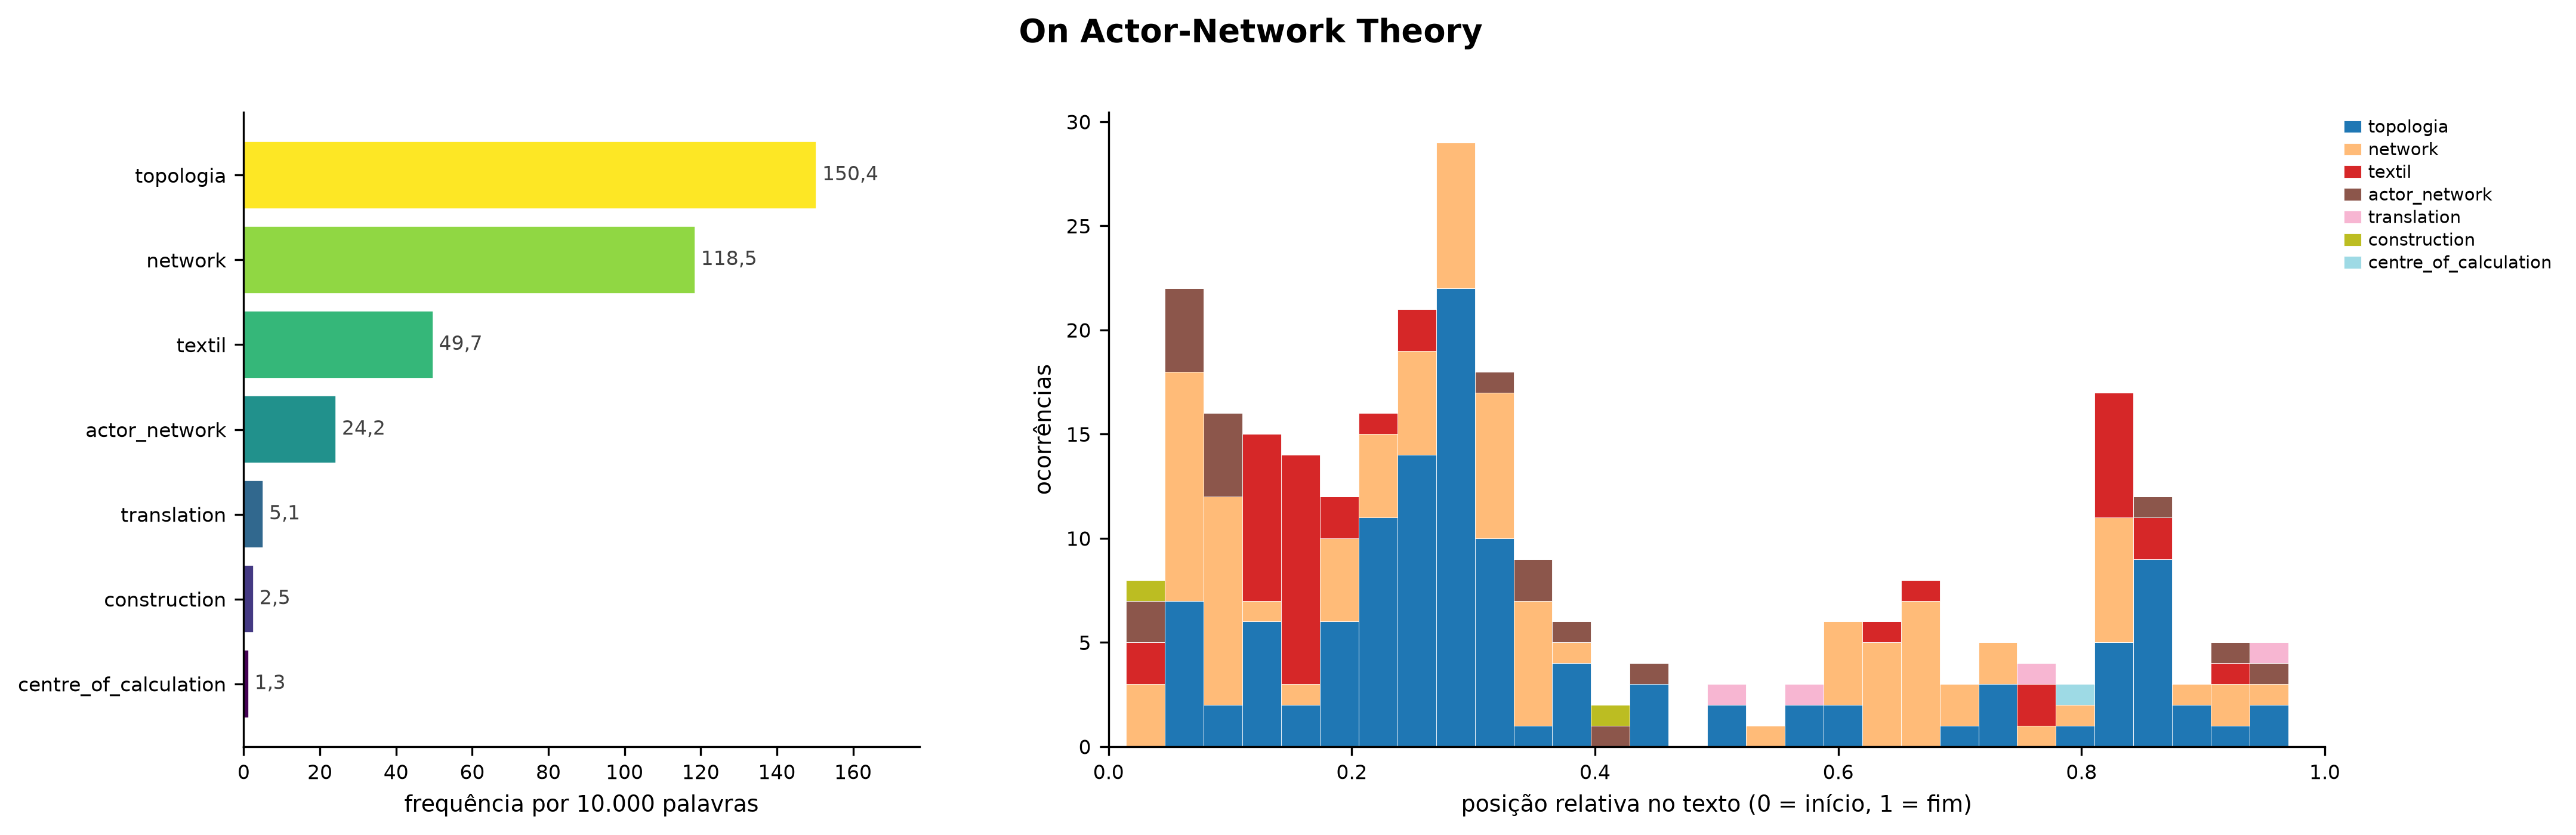
\includegraphics[width=1.0\linewidth]{figuras/cap.2/lexicometria/etapa2_clarifications_freq_e_densidade.png}
\caption[Frequência e distribuição dos rótulos em \emph{Clarifications}]{Rótulos do catálogo lexical em \emph{On Actor-Network Theory: A Few Clarifications} (Latour, 1996). À esquerda, a frequência de cada rótulo em ocorrências por dez mil palavras; à direita, a distribuição das ocorrências ao longo do texto. O artigo soma 276 ocorrências catalogadas, número que já desconta as três ocorrências brutas do rótulo \texttt{militar}. Os rótulos \texttt{topologia} e \texttt{network} dominam o artigo. O rótulo \texttt{militar} aparece com densidade zero, porque as suas ocorrências brutas foram classificadas, por leitura figural, em uso não-figurativo, e a barra do rótulo foi zerada na figura. A distribuição ao longo do texto é homogênea, sem picos localizados, em razão da extensão curta do artigo. Fonte: análise das figurações em \url{github.com/julianehelanski/analise-figuracoes-latour}.}
\label{fig:freq_densidade_clarifications}
\end{figure}

Em \emph{On Recalling ANT}, o mesmo deslocamento se confirma, e a Figura~\ref{fig:freq_densidade_recalling} mostra que a frequência dos rótulos no artigo repete o padrão metateórico de \emph{Clarifications}, com \texttt{topologia} e \texttt{network} no topo e o rótulo \texttt{militar} em densidade zero depois da leitura figural das suas ocorrências. Latour formula a teoria ator-rede como teoria \enquote{flat and folded} em que \enquote{there is no change of scale} \parencite[p.~17]{Latour1999RecallingANT}, e abandona o vocabulário das provas de força para descrever o que a teoria é: \enquote{may be the social possesses the bizarre property of not being made of agency and structure at all, but rather of being a \emph{circulating} entity} \parencite[p.~17]{Latour1999RecallingANT}. A circulação substitui a prova de força, o dobramento substitui a mobilização, o plano substitui o campo de batalha. Em outra passagem do mesmo artigo, ao formular a autocrítica sobre a contaminação do vocabulário que mobilizo desde a abertura deste capítulo~\ref{capitulo2}, Latour situa três dos quatro termos canônicos da teoria, \textit{translation}, \textit{alliance} e \textit{obligatory passage point}, em um vocabulário em que o rótulo \texttt{militar} se mistura com o rótulo \texttt{topologia}: \textit{alliance} é militar, \textit{translation} é têxtil-topológica, \textit{obligatory passage point} é topológico, e \textit{association} é o termo neutro que Latour propõe como melhor candidato \parencite[p.~20]{Latour1999RecallingANT}. A mistura é em si empiricamente significativa: o próprio Latour, ao revisar o vocabulário que herdou de \emph{Science in Action}, hesita entre a figuração militar e a têxtil-topológica e propõe substituições que vão na direção desta última.

\begin{figure}[htbp]
\centering
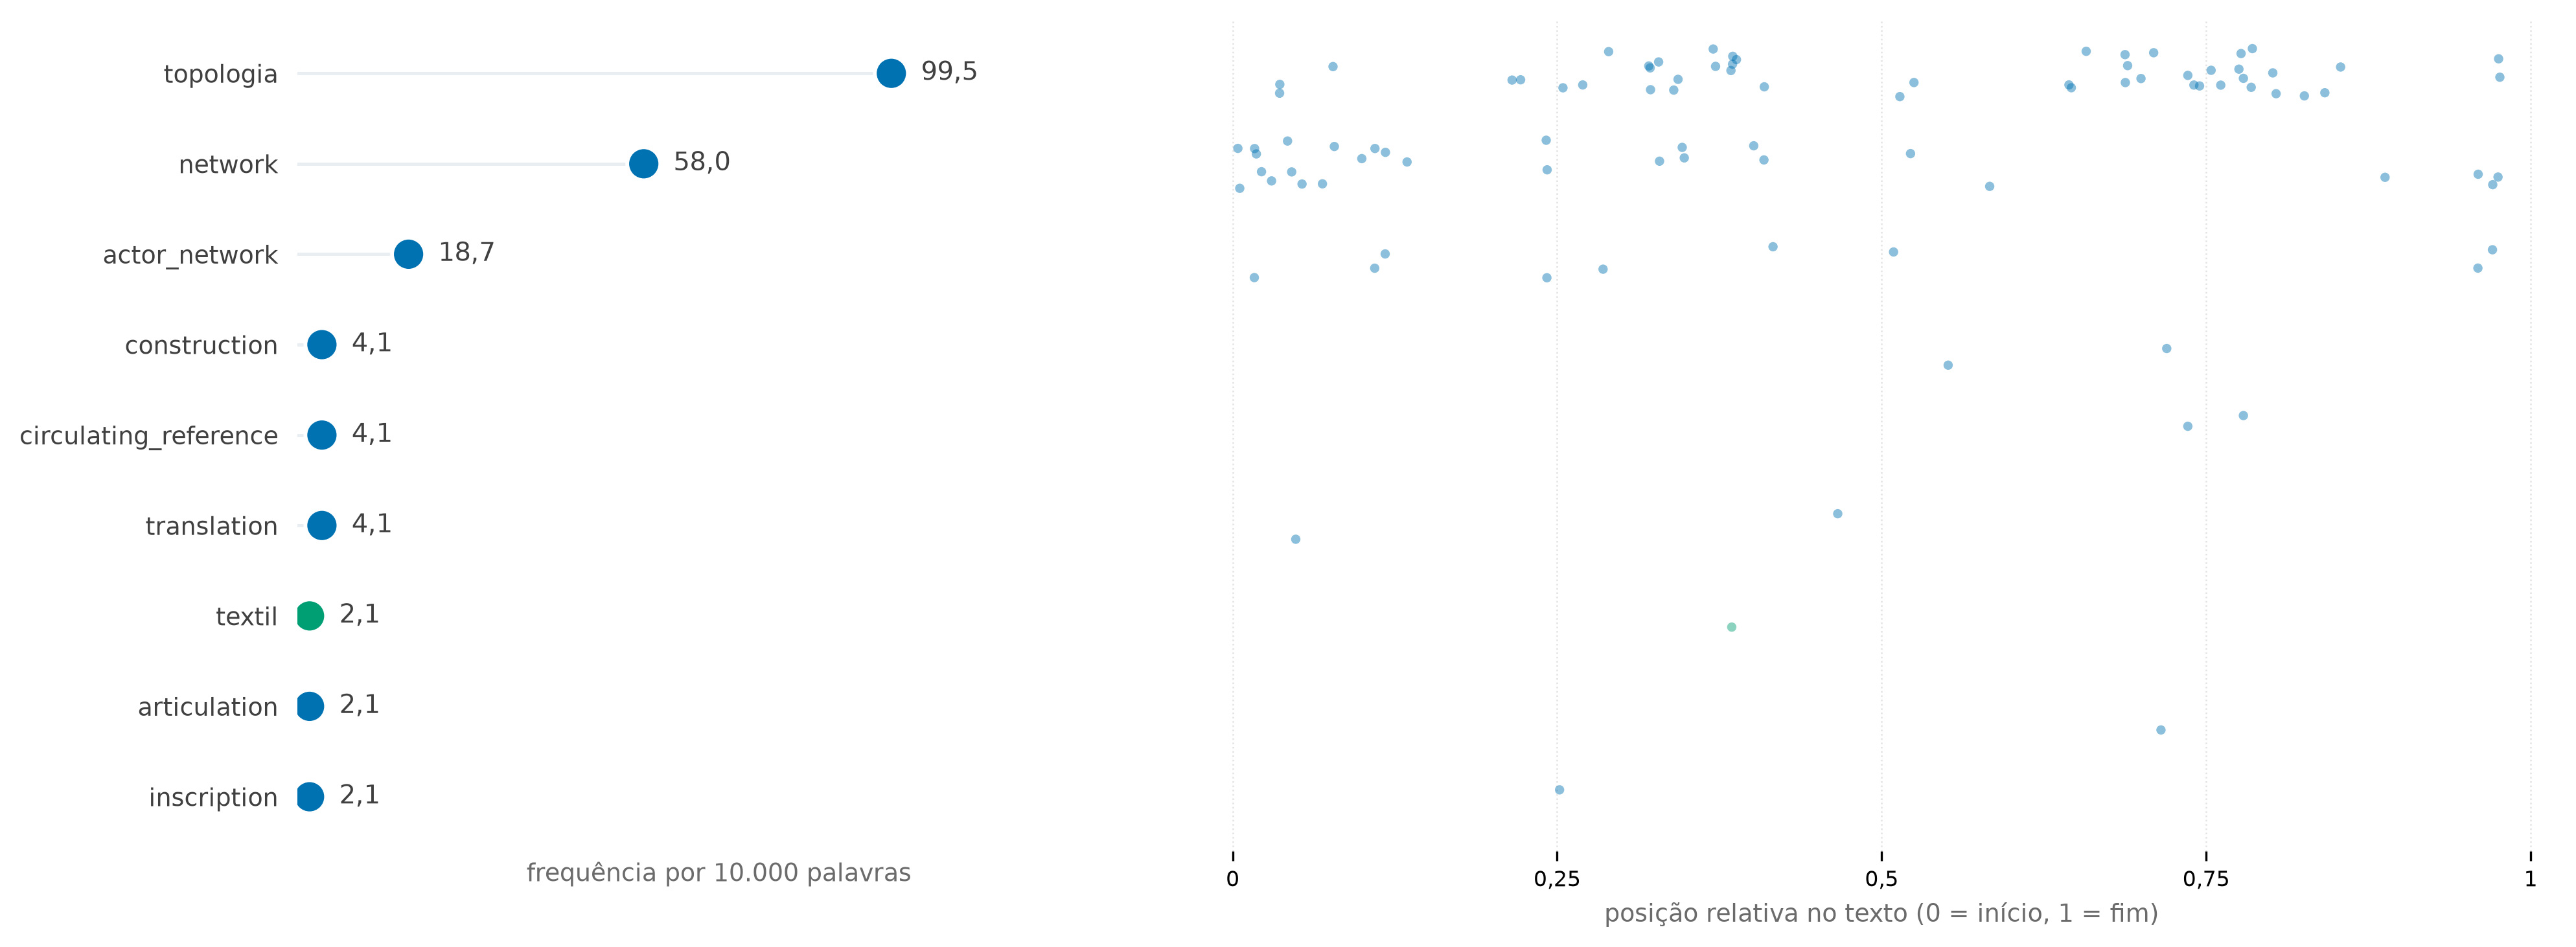
\includegraphics[width=1.0\linewidth]{figuras/cap.2/lexicometria/etapa2bis_recalling_integral_freq_e_densidade.png}
\caption[Frequência e distribuição dos rótulos em \emph{On Recalling ANT}]{Rótulos do catálogo lexical em \emph{On Recalling ANT} (Latour, 1999), sobre o corpus integral da etapa~2-bis. À esquerda, a frequência de cada rótulo em ocorrências por dez mil palavras; à direita, a distribuição das ocorrências ao longo do texto. O número de ocorrências catalogadas exibido no título da figura já desconta as duas ocorrências brutas do rótulo \texttt{militar}. Os rótulos \texttt{topologia} e \texttt{network} dominam o artigo, no mesmo padrão metateórico de \emph{Clarifications}. O rótulo \texttt{militar} aparece com densidade zero, pela mesma leitura figural: as duas ocorrências brutas foram classificadas em uso não-figurativo, e a barra do rótulo foi zerada na figura. A distribuição ao longo do texto é homogênea, sem picos localizados, em razão da extensão curta do artigo. Fonte: análise das figurações em \url{github.com/julianehelanski/analise-figuracoes-latour}.}
\label{fig:freq_densidade_recalling}
\end{figure}

A contagem em densidade relativa, mesmo refinada, ainda mede ocorrências do termo no texto sem distinguir os usos figurais dos usos polissêmicos ou citacionais. Para refinar essa distinção, fiz uma validação amostral semântica sobre as ocorrências dos quatro rótulos centrais nos dois artigos, \texttt{textil}, \texttt{topologia}, \texttt{network} e \texttt{actor\_network}, e classifiquei cada ocorrência amostrada em uso figural, parcialmente figural ou não-figural.\footnote{Fiz a validação amostral em três camadas: cinco ocorrências por rótulo com a janela KWIC mais densa em termos do mesmo rótulo, cinco ocorrências aleatórias por rótulo com semente fixa, e cinco ocorrências por rótulo cuja variante exata é das menos frequentes. Para rótulos com menos de quinze ocorrências, a amostra foi exaustiva. A taxa de figuralidade corresponde à fração ponderada de classificações \emph{figural} sobre o total da amostra do rótulo na obra.} Para \emph{Clarifications}, as taxas de figuralidade confirmam que o vocabulário aparece majoritariamente em uso figural, e não em polissemia residual: o rótulo \texttt{textil} tem taxa de 96,7\%, o rótulo \texttt{topologia} de 93,3\%, o rótulo \texttt{actor\_network} de 90\% e o rótulo \texttt{network} de 70\%. A inversão entre o registro militar dos livros monográficos e o registro têxtil-topológico do artigo metateórico sustenta-se, assim, já no plano figural depurado, para além do plano lexical bruto. Para o \emph{Recalling}, no corpus parcial da etapa~2, o refinamento produz um achado mais sutil: o rótulo \texttt{topologia} mantém taxa de figuralidade integral, mas os rótulos \texttt{network} e \texttt{actor\_network} caem de modo acentuado. A queda indica que, no estrato então processável, as ocorrências de \texttt{network} aparecem em registro predominantemente metalinguístico, com Latour citando o termo \enquote{network} para discutir o que ele significa, mais do que mobilizando o termo para descrever uma rede em ação, e que o rótulo \texttt{actor\_network} ali aparece em uso citacional. O que sobrevive ao refinamento no \emph{Recalling} parcial é o vocabulário topológico denotativo, \textit{flat}, \textit{folded}, \textit{scale}, \textit{circulating}, \textit{flow}, \textit{node} e \textit{connection}, que aparece em registro figural pleno e organiza a redescrição da teoria ator-rede que Latour propõe.

O argumento que sustento é o seguinte: a figuração militar-industrial em Latour é uma figuração de registro descritivo, que aparece quando o objeto da descrição é a tecnociência em ação, enquanto a uma figuração têxtil-topológica é figuração de registro metateórico, utilizada quando o objeto da descrição é a teoria que descreve essa tecnociência. A tensão entre os dois registros atravessa a obra, e o próprio Latour alterna entre os dois conjuntos conforme o objeto que descreve. Dentro do gênero metateórico, a validação amostral semântica identifica ainda uma divisão de segundo nível: \emph{Clarifications} se mantém em registro expositivo-figural, com taxa de figuralidade agregada de 0,875, enquanto \emph{On Recalling ANT} se inscreve em registro autocrítico-metalinguístico, com taxa de 0,636, sustentada pela concentração metalinguística em torno do termo \texttt{network} que Latour tematiza para suspender. O que este capítulo propõe para a tese em geral, em coerência com o gesto assumido na abertura deste capítulo~\ref{capitulo2}, é manter ativas essas figurações na escrita que descreve ao mesmo tempo a tecnociência em ação e a teoria que a descreve. O capítulo~\ref{capitulo3}, ao descrever a rede do \texttt{C4AI} e da \texttt{IBM} que recruta aliados e descreve provas de força, se mantém predominantemente pelo figuração militar-industrial. O capítulo~\ref{capitulo1}, em registro reflexivo sobre a minha própria escrita, se mantém predominantemente nas figurações têxteis, trama, costura, retalho, e essa escolha, que não foi intencional, reflete o que identifiquei na análise lexicométrica das obras de Latour: o vocabulário têxtil é o vocabulário do registro metateórico, e é esse o registro de escrita e de descrição em que o capítulo~\ref{capitulo1} se inscreve. O capítulo~\ref{capitulo4} ocupa uma posição distinta dessa. Ele se faz em registro misto, porque mantém o léxico latouriano da cadeia de translação e da inscrição que organiza também o capítulo~\ref{capitulo3}, e ao mesmo tempo descreve a tecnociência do \texttt{Spira} por meio de figurações têxteis e topológicas, fio, nó, conexão, topologia fluida, objeto fracional. Levar essas figurações à descrição de uma prática tecnocientífica, que pelo padrão que identifiquei na obra de Latour pediria o registro militar-industrial, constitui uma experimentação. Por experimentação entendo a tentativa de observar, descrever, interpretar, analisar e propor a tecnociência por um arranjo de figurações diferente do que o campo dos estudos de ciência e tecnologia mobiliza com mais frequência, e a tensão entre o léxico latouriano e as figurações têxteis é uma parte dessa experimentação. O exercício foi difícil, e a dificuldade tem a forma que o próprio Latour reconheceu em \emph{On Recalling ANT}. Ao admitir que o vocabulário da teoria ator-rede contaminou a capacidade de deixar os atores construírem o seu próprio espaço, Latour diagnostica que o problema, para ele, foi um vocabulário \enquote{not poor enough}, pobre mas ainda insuficientemente pobre, e conclui que projetar um espaço para que os atores desdobrem as suas próprias categorias é \enquote{a much harder task than we thought at first} \parencite[p.~20--21]{Latour1999RecallingANT}. No mesmo movimento, Latour recorre a outras figurações para nomear o que a teoria deveria ser, e cita o conceito \enquote{fluid}, de Law e Mol, ao lado de outras imagens de trilha e de coreografia. O próprio Latour, no momento em que reconhece o limite do léxico que construiu, busca figurações novas, e as busca no vocabulário têxtil-topológico que esta tese rastreia. Deixar os actantes falarem por si é mais difícil do que parece, e talvez por isso seja preciso recorrer a novos modos de pensamento e a novas figurações para descrever, analisar e imaginar as práticas tecnocientíficas. Foi essa dificuldade que encontrei ao longo da escrita desta tese, e ela se manifesta de modo peculiar na maneira como a comecei e em cada uma das tramas tecnoetnográficas que desenvolvi, esta do capítulo~\ref{capitulo2} e as dos capítulos~\ref{capitulo3} e~\ref{capitulo4}.

Cabe mencionar, ainda, um achado complementar que se faz em escala menor e que leva o argumento em outra direção. A segunda edição de \emph{Laboratory Life}, de 1986, acrescentou ao texto da primeira edição, de 1979, um \emph{Postscript} em que Latour e Woolgar fazem balanço retrospectivo do construtivismo social e respondem a críticas. A distribuição dos rótulos dentro desse \emph{Postscript} sustenta, em escala intra-obra, o mesmo padrão que o conjunto de cinco obras sustenta em escala maior. O rótulo \texttt{construction} concentra 13,39 ocorrências por dez mil palavras no \emph{Postscript}, densidade próxima do valor de 19,29 que o rótulo registra no livro inteiro, e que faz de \emph{Laboratory Life} a obra do meu corpus com maior densidade desse campo. A presença do construtivismo no \emph{Postscript} não surpreende: o gênero retrospectivo do \emph{Postscript} é o espaço em que Latour e Woolgar defendem a posição construtivista que organizou o livro. O rótulo \texttt{construction} é, em escala menor, o que o vocabulário têxtil-topológico é em escala maior: vocabulário de registro autorreflexivo, mobilizado quando o objeto da descrição muda da prática para a teoria. O achado pequeno sustenta o achado maior: a autorreflexão muda o vocabulário, e o vocabulário muda conforme o registro em que se escreve.

A etapa~2 e a etapa~2-bis entregaram dois resultados que reorganizam as figurações da obra latouriana. O primeiro é a confirmação refinada por desambiguação, co-ocorrência e validação amostral semântica, de que a figuração militar-industrial é uma figuração situada que aparece de modo seletivo conforme o objeto descrito, e que se ausenta onde a descrição neutra a manteria. O segundo é a demonstração de que a metáfora têxtil-topológica, que reconheço como figuração feminista cujo início mais marcante se deu com Haraway e com a tradição que reconstitui essas figurações associadas ao trabalho de mulheres, é figuração que Latour mesmo compõe em seus momentos autorreflexivos, e que coexiste com a figuração militar-industrial. Assim, a tensão entre figurações que organiza este capítulo encontra, a partir da análise textual, evidências de que ela atravessa a obra latouriana de dentro para fora.

O que nos leva, então, à próxima questão: se as figurações que sustentam a teoria ator-rede são limitadas ou mesmo inadequadas, de que modo descrever, explicar e propor a tecnociência --- neste caso, a pesquisa em IA e acerca de sistemas de IA --- sem reiterar os modos de pensamento das figurações do \textit{front}?

\subsection{A figuração em \emph{An Inquiry into Modes of Existence}}
\label{subsec:figuracao_aime}

Encerro a análise lexicométrica com \emph{An Inquiry into Modes of Existence} (\textit{AIME}), obra na qual Latour repensa a teoria ator-rede de um modo inteiramente novo.\footnote{Cito o livro pela tradução de Catherine Porter publicada pela Harvard University Press em 2013 sob o título \emph{An Inquiry into Modes of Existence: An Anthropology of the Moderns} \parencite{Latour2013Inquiry}. O original em francês, \emph{Enquête sur les modes d'existence}, saiu pela La Découverte em 2012, e a tradução brasileira, \emph{Investigação sobre os modos de existência: uma antropologia dos modernos}, em tradução de Alexandre Agabiti Fernandez, foi publicada pela Editora Vozes em 2019 \parencite{Latour2019Investigacao}. A escolha pelo texto em inglês para a análise lexicométrica é coerente com a etapa 1, em que processei originais ou versões anglo-saxônicas de cada obra de Latour, e com a etapa 2, em que processei os artigos em inglês de 1996 e 1999. As legendas em português dos elementos do quadro 1 que apresento adiante são tomadas da tradução de Agabiti Fernandez, e as legendas em inglês das pp.~487--488 da edição da Harvard. A análise integral está documentada em \url{github.com/julianehelanski/analise-figuracoes-latour/blob/main/outputs/etapa3_aime/relatorio_etapa3.md}.} \emph{AIME} é o livro no qual a criatura de Latour sai do caixão. A teoria ator-rede que ele dissera ter enterrado em \textit{On Recalling ANT}, com quatro pregos e uma estaca no coração, retorna em \textbf{AIME} como ponto de partida de uma investigação ampliada, escrita sob a figura ficcional de uma antropóloga que vai a campo entre os Modernos para reconstituir o sistema de valores das sociedades ocidentais \parencite[p.~28]{Latour2013Inquiry}.\footnote{Latour formula a metáfora dos quatro pregos no caixão para criticar os quatro elementos que compõem a expressão \enquote{teoria ator-rede}. As palavras teoria, ator, rede e o hífen que liga as duas últimas são, na sua leitura, os quatro pregos. A palavra rede (\textit{network}) perdeu seu caráter crítico depois da popularização da internet, e passou a significar transporte sem deformação e acesso instantâneo, o oposto do que a TAR pretendia. A palavra ator (\textit{actor}), ligada à palavra rede pelo hífen, deu margem a mal-entendidos como a dicotomia entre agência e estrutura, na qual a TAR tampouco pretendia entrar. A palavra teoria (\textit{theory}) foi outro equívoco: Latour, citando Mike Lynch, escreve que a TAR deveria ter sido chamada de \enquote{ontologia actante-rizoma} (\textit{actant-rhizome ontology}), mas que ele achou a expressão horrível e o acrônimo \texttt{ARO} pior ainda; além disso, a TAR nunca foi \enquote{uma teoria explicativa do social, mas um método para aprender com os próprios atores} \parencite[p.~19]{Latour1999RecallingANT}. O hífen, por fim, é um lembrete infeliz do debate entre agência e estrutura no qual os autores nunca quiseram entrar. Latour declara, então, ter enterrado sua criatura com quatro pregos e uma estaca no coração, ainda que \enquote{algo leve e belo} pudesse emergir como conquista coletiva futura \parencite{Latour1999RecallingANT}.} 

No capítulo 12 do \textbf{AIME}, Latour afirma: \enquote{the actor-network theory, which the present inquiry seeks to complete} \parencite[p.~353]{Latour2013Inquiry}. O AIME não substitui a teoria ator-rede; complementa-a. A formulação que motiva essa extensão aparece no capítulo 1 do livro, em que a antropóloga ficcional que Latour faz seguir o AIME descobre, no movimento mesmo da pesquisa, a limitação que organiza o resto da \emph{Inquiry}: \enquote{networks [net] have a limitation: they do not qualify values} \parencite[p.~35]{Latour2013Inquiry}. Discuti os limites da teoria ator-rede no capítulo~\ref{capitulo1}, por meio da proposição complementar de cortar e costurar redes com Strathern, Barad, Haraway, Costa e Law. Para a análise lexicométrica que faço aqui, a AIME consiste em uma continuação crítica da teoria ator-rede, por isso, inclui essa obra no corpus; e também por partir e repensar a teoria ator-rede nesta tese. 

\subsubsection{O quadro 1 e a metalinguagem da investigação}
\label{subsubsec:aime_quadro1}

Inicio a análise de \textit{An Inquiry into Modes of Existence} retomando o gesto que o próprio Latour realiza ao final da obra \parencite[pp.~487--488]{Latour2013Inquiry}, em que ele reúne em uma tabela o estado da sua investigação em quinze modos e nas cinco perguntas canônicas que cada modo deve responder. A edição brasileira \parencite[pp.~392--393]{Latour2019Investigacao} traz a tabela com o título \emph{quadro 1: Resumo do estado da investigação} e organiza as quinze linhas em cinco grupos: \enquote{Sem quase-objeto e sem quase-sujeito} (reprodução, metamorfose, hábito), \enquote{Quase-objetos} (técnica, ficção, referência), \enquote{Quase-sujeitos} (política, direito, religião), \enquote{Vínculos entre quase-objetos e quase-sujeitos} (apego, organização, moral) e \enquote{Metalinguagem da investigação} (rede, preposição, duplo clique). As cinco perguntas canônicas que organizam as colunas do quadro orientam a obra de Latour: o \emph{hiato} (\emph{hiatus}) é a descontinuidade característica de cada modo, o ponto em que algo se interrompe e precisa ser retomado por outra caminho; a \emph{trajetória} (\emph{trajectory}) é o movimento específico pelo qual cada modo atravessa esse hiato sem suprimi-lo; as \emph{condições de felicidade e infelicidade} (\emph{felicity and infelicity conditions}) são os critérios que distinguem, em cada modo, o uso bem-sucedido do uso mal-sucedido, e que Latour adota da teoria dos atos de fala de J. L. Austin para qualificar os valores que a rede sozinha não distinguiria; os \emph{seres a instaurar} (\emph{beings to institute}) são as entidades que cada modo faz existir quando a sua trajetória se cumpre; e a \emph{alteração} (\emph{alteration}) é a forma de ser-outro que cada modo institui, em coerência com a tese ontológica do livro de que existir é, sempre, ser-outro de algum modo. O Grupo~5, \emph{Metalinguagem da investigação}, ressoa com a questão da figuração: nesse grupo Latour situa o \enquote{modo rede} ao lado da \enquote{preposição} e do \enquote{duplo clique}, e é esse deslocamento que direciona a análise que faço nesta subseção. A tabela~\ref{tab:aime_quadro1_grupo5} reproduz esse grupo.

\begin{table}[!htb]
\centering
\caption[Grupo 5 do quadro 1 de AIME: a metalinguagem da investigação]{Grupo~5 do quadro~1 de \emph{An Inquiry into Modes of Existence} \parencite{Latour2013Inquiry}: três modos cuja função é dar conta da própria investigação. As seis colunas seguem o quadro~1: o nome do modo e as cinco perguntas canônicas a que cada modo responde. Transcrição minha da edição inglesa, sobre a qual fiz a análise lexicométrica.}
\label{tab:aime_quadro1_grupo5}
\footnotesize
\begin{tabular}{p{1.4cm}p{1.9cm}p{2.0cm}p{2.6cm}p{1.9cm}p{2.0cm}}
\toprule
Name & Hiatus & Trajectory & Felicity and infelicity conditions & Beings to institute & Alteration \\
\midrule
\texttt{[NET]} network & Surprise of association & Following heterogeneous connections & Traverse domains / lose freedom of inquiry & Networks of irreductions & Extend associations \\
\addlinespace
\texttt{[PRE]} preposition & Category mistakes & Detection of crossings & Give each mode its template / crush the modes & Interpretive keys & Ensure ontological pluralism \\
\addlinespace
\texttt{[DC]} double click & Horror of hiatuses & Displacement without translation & Speak literally / speak through figures and tropes & Reign of indisputable Reason & Maintain the same despite the other \\
\bottomrule
\end{tabular}
\end{table}

A teoria ator-rede, que Latour designa pela sigla \texttt{[NET]} em inglês e \texttt{[RES]} em português, e que organizou a descrição da prática tecnocientífica nos três livros e nos dois artigos metateóricos analisados na primeira etapa da análise lexicométrica, aparece em \textit{AIME} sob nova função, como uma das três formas da \enquote{metalinguagem da investigação} (\textit{metalanguage}) que compõem o Grupo 5 do quadro 1.\footnote{O termo \emph{metalanguage} aparece vinte e uma vezes ao longo do corpo de \textit{AIME} em uso teórico pleno. A escolha de não incluir o termo no catálogo da etapa  3 segue o critério que rege esta etapa: o catálogo rastreia o vocabulário figurativo identificado pela leitura qualitativa de \textit{AIME}, e não os rótulos dos grupos que organizam o quadro 1. Registro a presença lexical do termo como observação que abre caminho para uma ampliação futura do catálogo.} A oposição entre \emph{metalanguage} e \emph{infralanguage}, com que Latour qualifica essa metalinguagem, já havia sido estabilizada em \emph{On Actor-Network Theory: A Few Clarifications}, em que Latour escreve que o vocabulário da TAR é \enquote{more an infralanguage than a metalanguage} e que essa infralinguagem \enquote{has to be poor, limited, short and simple} \parencite[p.~\texttt{[p. 7]}]{latour1996clarifications}. Em \textit{AIME}, a oposição se mantém em termos semelhantes: Latour descreve a preposição como \enquote{a metalanguage for this inquiry --- or, better, an infralanguage} \parencite[p.~263]{Latour2013Inquiry}, e prefere \enquote{infralinguagem} porque \enquote{metalinguagem} sugere posição superior ou externa, enquanto a preposição se exerce de dentro da investigação, não de fora. O que muda entre o artigo e o \textit{AIME} é a função que a infralinguagem desempenha: em \emph{Clarifications} ela é a própria TAR como vocabulário pobre que se aplica de modo simétrico a todas as redes; em \textit{AIME} ela passa à preposição \texttt{[PRE]}, e a rede se torna ferramenta empírica, que Latour caracteriza no capítulo 1 do livro como \enquote{a tool that makes a positive empirical investigation possible} \parencite[p.~36]{Latour2013Inquiry} e que ganha estatuto metalinguístico no Grupo 5 ao deixar de ser modo descritivo. O terceiro modo do Grupo 5, o duplo clique \texttt{[DC]}, diz respeito à pretensão de uma metalinguagem universal que aboliria as descontinuidades entre os modos, e que Latour identifica como o adversário a desfazer. Os três modos ocupam, em consequência, lugares distintos: a preposição como infralinguagem por excelência, a rede como ferramenta empírica que ganha estatuto metalinguístico no \textit{AIME} ao deixar de ser modo descritivo, e o duplo clique como pretensão a recusar. O que motiva esse rearranjo é nomeado por Latour no capítulo 1 do \textit{AIME}, em que ele escreve que \enquote{networks have a limitation: they do not qualify values} \parencite[p.~35]{Latour2013Inquiry}: o vocabulário da rede registra as associações sem qualificá-las, e a investigação em modos de existência precisa de outro vocabulário para fazer essa qualificação. Esse outro vocabulário, que Latour distribui ao longo do livro inteiro e sistematiza retrospectivamente no quadro 1 e na Conclusão, é o que a leitura qualitativa que fiz de \textit{AIME} buscou capturar para construir o catálogo novo da etapa  3.\footnote{O catálogo novo da etapa  3 rastreia o vocabulário figurativo que a leitura qualitativa de \textit{AIME} identifica como específico do livro em relação às cinco obras anteriores, e não a taxonomia dos quinze modos de existência que organiza a arquitetura de \textit{AIME}. Os quinze modos, designados pelas siglas \texttt{[rep]}, \texttt{[met]}, \texttt{[hab]}, \texttt{[tec]}, \texttt{[fic]}, \texttt{[ref]}, \texttt{[pol]}, \texttt{[law]}, \texttt{[rel]}, \texttt{[att]}, \texttt{[org]}, \texttt{[mor]}, \texttt{[net]}, \texttt{[pre]} e \texttt{[dc]}, são a nomenclatura técnica com que Latour estrutura a sua investigação, e a sua exposição cabe à literatura especializada sobre \textit{AIME}, não à pergunta lexicométrica que faço aqui. A relação entre os doze rótulos do catálogo novo e o quadro 1 e a Conclusão de \textit{AIME}, documentada na tabela~\ref{tab:mapeamento_quadro1_catalogo_novo}, é de ancoragem textual retrospectiva, e não de derivação a priori. Os identificadores dos rótulos, assim como os identificadores das tabelas e figuras desta subseção, aparecem em inglês em coerência com o tratamento bilíngue do corpus que justifico na nota acima: os identificadores que reproduzem conceitos cunhados por Latour (\texttt{inscription}, \texttt{black\_box}, \texttt{network}) conservam o nome próprio do conceito, e os identificadores que correspondem a rótulos que eu mesma reuni a partir da leitura do corpus (\texttt{militar}, \texttt{textil}, \texttt{topologia}) são etiquetas analíticas minhas e seguem a forma com que constam no repositório.}

A tabela~\ref{tab:mapeamento_quadro1_catalogo_novo} apresenta o mapeamento entre os doze rótulos do catálogo novo e os elementos do quadro 1 e da Conclusão de \textit{AIME} em que cada rótulo encontra ancoragem textual. A correspondência é direta para a maior parte dos rótulos, e nos casos em que ela não é literal indico em coluna própria a passagem do livro em que cada rótulo se sustenta.

\begin{table}[!htb]
\centering
\caption[Mapeamento entre o catálogo novo da etapa  3 e o quadro 1 de AIME]{Mapeamento entre os doze rótulos do catálogo novo da etapa  3 da minha análise lexicométrica e os elementos do quadro 1 e da Conclusão de \textit{AIME} (\textcite{Latour2013Inquiry}, pp.~487--488; tradução brasileira em \textcite{Latour2019Investigacao}) em que cada rótulo encontra ancoragem textual. As três últimas linhas correspondem a vocabulários da Conclusão de \textit{AIME}, fora do quadro 1; as demais correspondem a colunas ou linhas do quadro. A coluna \enquote{ancoragem textual} indica a passagem do livro em que cada rótulo se sustenta, e foi conferida pela leitura do texto integral e pela validação cruzada com as ocorrências do KWIC. Fonte: elaboração própria a partir da leitura qualitativa de \textit{AIME} e da literatura sobre a guinada latouriana pós-2007, com ancoragem retrospectiva no quadro 1 e na Conclusão do livro. Análise lexicométrica documentada em \url{github.com/julianehelanski/analise-figuracoes-latour}.}
\label{tab:mapeamento_quadro1_catalogo_novo}
\small
\begin{tabular}{p{3.8cm}p{3.5cm}p{6.3cm}}
\toprule
Termo de Latour & Campo do catálogo novo & Ancoragem textual em \textit{AIME} \\
\midrule
\emph{Hiatus}                                  & \texttt{trajectory\_pass}     & coluna 2 do Quadro 1; cap.~1 sobre descontinuidades \\
\emph{Trajectory}                              & \texttt{trajectory\_pass}     & coluna 3 do Quadro 1; cap.~2 sobre \enquote{passes} \\
\emph{Felicity and infelicity conditions}      & \texttt{felicity}             & coluna 4 do Quadro 1; cap.~3 sobre condições de veridição \\
\emph{Beings to institute}                     & \texttt{institution}          & coluna 5 do Quadro 1; cap.~2 sobre instituição \\
\emph{Alteration}                              & \texttt{alteration}           & coluna 6 do Quadro 1; cap.~6 sobre ser-enquanto-outro \\
\emph{Name} (modo)                             & \texttt{modes\_of\_existence} & colunas 1 e 7 do Quadro 1; subtítulo do livro \\
\emph{Category mistake} / \emph{domain}        & \texttt{domain\_category}     & cap.~2 sobre o método dos cruzamentos; cap.~1 sobre domínios \\
\emph{The Moderns}                             & \texttt{moderns}              & subtítulo do livro; cap.~1 sobre a antropologia dos modernos \\
\texttt{[PRE]} \emph{preposition} (Grupo 5)    & \texttt{preposition}          & linha 14 do Quadro 1; cap.~3 sobre chaves interpretativas \\
\emph{Negotiation over values} (Conclusão)     & \texttt{values}               & cap.~16 e Conclusão; cap.~9 sobre apego \\
\emph{Diplomatic arrangement} (Conclusão)      & \texttt{diplomacy}            & Conclusão; cap.~14 sobre o cosmos \\
\emph{Gaia} (Conclusão)                        & \texttt{gaia}                 & Conclusão e cap.~16 sobre a era do Antropoceno \\
\bottomrule
\end{tabular}
\end{table}

O mapeamento da tabela~\ref{tab:mapeamento_quadro1_catalogo_novo} sustenta o catálogo novo da etapa  3 em dois apoios independentes: a leitura qualitativa que identifica os rótulos a partir das ocorrências no texto, e o vocabulário que o próprio Latour estabilizou no quadro 1 e na Conclusão de \textit{AIME}. A coincidência entre a leitura e os elementos catalogados por Latour confirma que o vocabulário identificado pela leitura corresponde ao que o livro sistematiza retrospectivamente nas suas duas estruturas de fechamento.

O mapeamento esclarece também a posição do rótulo \texttt{network} do catálogo antigo na análise que apresento a seguir. As 255 ocorrências do rótulo \texttt{network} em \textit{AIME}, em densidade comparável à dos livros da etapa 1, sustentam uma continuidade lexical que oculta uma descontinuidade de função: a rede que em \emph{Science in Action} compunha a gramática descritiva da prática tecnocientífica é, em \textit{AIME}, um instrumento da antropóloga ficcional para detectar as associações heterogêneas entre os modos. O Grupo 5 do quadro 1 torna essa descontinuidade visível, ao situar a rede ao lado da preposição e do duplo clique, no grupo dos modos que dão conta da própria investigação, e não no grupo dos modos descritivos. A análise das tabelas seguintes mede a continuidade lexical do termo, e a leitura interpretativa que faço dessas tabelas reconhece a descontinuidade de função que está por trás dela.

Sigo, em consequência, dois catálogos aplicados em paralelo na análise de \textit{AIME}. O primeiro é o catálogo de dezenove rótulos das etapas 1 e 2, que aplico a \textit{AIME} para permitir a comparação direta com as cinco obras anteriores. O segundo é o catálogo de doze rótulos da etapa 3, que construí a partir da leitura qualitativa de \textit{AIME} e da literatura sobre a obra tardia de Latour, e que encontra ancoragem retrospectiva no quadro 1 e na conclusão do livro conforme a tabela~\ref{tab:mapeamento_quadro1_catalogo_novo}. A construção do catálogo novo exigiu algumas decisões de depuração, porque vários dos termos que apareciam na leitura têm na língua inglesa usos polissêmicos: \emph{value} pode ser axiológico ou econômico, \emph{mode} pode ser nome técnico ou substantivo comum, \emph{modern} pode ser adjetivo descritivo ou nome próprio dos modernos, \emph{Earth} pode ser planeta ou solo fértil. Cada um desses termos passou por uma decisão de inclusão ou exclusão, que privilegia as expressões em que Latour usa o termo em sentido técnico próprio do livro.\footnote{As decisões pontuais de depuração de cada rótulo, com as variantes mantidas e as variantes retiradas, estão registradas no arquivo \texttt{campos\_lexicais/catalogo\_termos\_aime.yaml} do repositório, em \url{github.com/julianehelanski/analise-figuracoes-latour}. A polissemia residual dos termos \emph{experience}, \emph{crossing}, \emph{domain} e \emph{value} carrega ruído que a contagem bruta reflete, e a leitura interpretativa precisa considerá-lo. A aplicação do catálogo novo apenas a \textit{AIME}, e não retroativamente às cinco obras anteriores, decorre da origem do catálogo: os doze rótulos correspondem a vocabulário específico de \textit{AIME} identificado pela leitura qualitativa, e o rendimento esperado da aplicação retroativa nos textos de 1986 a 1999 seria de ordem de grandeza inferior ao ruído.} O corpus de \textit{AIME} passou pelas mesmas etapas de saneamento que apliquei às outras obras, descritas em detalhe no repositório.

\begin{longtable}{@{}p{0.23\textwidth} p{0.23\textwidth} p{0.46\textwidth}@{}}
\caption[Catálogo lexical da etapa 3 (AIME)]{Catálogo lexical da etapa 3 (\textit{AIME}, 2013): os doze rótulos identificados pela leitura qualitativa do livro e da literatura sobre a obra tardia de Latour, com a ancoragem textual de cada campo no quadro 1 e na conclusão de \textit{AIME} e uma amostra dos termos que o definem. A amostra segue a ordem do arquivo de definição: rótulos com até oito termos aparecem completos, rótulos maiores trazem os oito primeiros termos seguidos de \enquote{entre outros}. A lista completa está no repositório, em \texttt{campos\_lexicais/catalogo\_termos\_aime.yaml}, em \url{github.com/julianehelanski/analise-figuracoes-latour}.}\label{tab:catalogo-etapa3}\\
\toprule
Campo & Ancoragem textual em \textit{AIME} & Amostra de termos do catálogo \\
\midrule
\endfirsthead
\caption[]{Catálogo lexical da etapa  3 (\textit{AIME}) (continuação).}\\
\toprule
Campo & Ancoragem textual em \textit{AIME} & Amostra de termos do catálogo \\
\midrule
\endhead
\midrule
\multicolumn{3}{r@{}}{\footnotesize continua na próxima página}\\
\endfoot
\bottomrule
\endlastfoot
\texttt{modes\_of\_existence} & Quadro 1 / Conclusão & \texttt{mode of existence}, \texttt{modes of existence} \\
\texttt{preposition} & Quadro 1 / Conclusão & \texttt{preposition}, \texttt{prepositions}, \texttt{prepositional} \\
\texttt{felicity} & Quadro 1 / Conclusão & \texttt{felicity}, \texttt{infelicity}, \texttt{felicity condition}, \texttt{infelicity condition}, \texttt{felicity conditions}, \texttt{infelicity conditions}, \texttt{felicitous}, \texttt{infelicitous} \\
\texttt{diplomacy} & Quadro 1 / Conclusão & \texttt{diplomatic}, \texttt{diplomat}, \texttt{diplomats}, \texttt{diplomacy}, \texttt{negotiation}, \texttt{negotiations}, \texttt{negotiating}, \texttt{negotiate}, entre outros \\
\texttt{gaia} & Quadro 1 / Conclusão & \texttt{Gaia}, \texttt{Anthropocene}, \texttt{terrestrial}, \texttt{ecology}, \texttt{ecological}, \texttt{ecologies}, \texttt{climate}, \texttt{climatologist}, entre outros \\
\texttt{values} & Quadro 1 / Conclusão & \texttt{qualify values}, \texttt{qualifies values}, \texttt{qualifying values}, \texttt{qualified values}, \texttt{value system}, \texttt{values system}, \texttt{system of values}, \texttt{qualify} \\
\texttt{trajectory\_pass} & Quadro 1 / Conclusão & \texttt{trajectory}, \texttt{trajectories}, \texttt{course of action}, \texttt{hiatus}, \texttt{discontinuity}, \texttt{discontinuities}, \texttt{continuity}, \texttt{continuities}, entre outros \\
\texttt{institution} & Quadro 1 / Conclusão & \texttt{instituting}, \texttt{institute}, \texttt{institutes}, \texttt{instituted}, \texttt{institution}, \texttt{institutions} \\
\texttt{domain\_category} & Quadro 1 / Conclusão & \texttt{category mistake}, \texttt{category mistakes}, \texttt{domain}, \texttt{domains}, \texttt{crossing}, \texttt{crossings} \\
\texttt{moderns} & Quadro 1 / Conclusão & \texttt{Moderns}, \texttt{modernity}, \texttt{modernizing}, \texttt{modernism}, \texttt{modernization} \\
\texttt{alteration} & Quadro 1 / Conclusão & \texttt{alteration}, \texttt{alterations}, \texttt{alter}, \texttt{altered}, \texttt{alters}, \texttt{altering}, \texttt{being-as-other}, \texttt{being-as-another}, entre outros \\
\texttt{experience} & Quadro 1 / Conclusão & \texttt{experience}, \texttt{experiences}, \texttt{experienced}, \texttt{experiential}, \texttt{empirical} \\
\end{longtable}

A contagem do catálogo das etapas 1 e 2 aplicada a \textit{AIME} sustenta dois achados que articulo em sequência. O primeiro é a continuidade do vocabulário têxtil-topológico em densidade intermediária, com reorganização lexical interna. A densidade do rótulo \texttt{topologia} em \textit{AIME} (26,43 por dez mil palavras) coloca a obra no mesmo patamar de \emph{Science in Action} (34,68) e \emph{Pandora's Hope} (27,58), abaixo das densidades extraordinárias dos artigos, em parte inflacionadas pela tamanho menor do corpus em que aparecem. Em valor absoluto, \textit{AIME} registra 514 ocorrências do rótulo \texttt{topologia}, número maior do que em qualquer das obras anteriores, e o livro mobiliza o vocabulário topológico em volume que faz dele o rótulo mais denso da obra inteira. As variantes \emph{top} do rótulo \texttt{topologia} em \textit{AIME} são \emph{path} (90), \emph{trajectory} (61), \emph{outside} (55), \emph{trajectories} (34) e \emph{paths} (33), em diferença com \emph{Science in Action} e \emph{Pandora's Hope}, em que dominavam \emph{inside}, \emph{outside}, \emph{scale} e \emph{flow}. O vocabulário topológico em \textit{AIME} se reorganiza em torno do par \emph{path}/\emph{trajectory}, que se articula com o rótulo novo \texttt{trajectory\_pass} que apresento adiante. O rótulo \texttt{network} em \textit{AIME} (13,11 por dez mil palavras) é o mais alto entre as obras do corpus, superando os 4,26 de \emph{Laboratory Life}, os 9,08 de \emph{Science in Action} e os 2,73 de \emph{Pandora's Hope}, e fica em ordem de grandeza intermediária entre os livros e os artigos metateóricos. O rótulo \texttt{textil} em \textit{AIME} (10,34 por dez mil) registra densidade comparável à dos livros (7,94 e 8,20). O vocabulário têxtil-topológico permanece em \textit{AIME}, portanto, em densidade intermediária, sem o pico dos artigos metateóricos e sem o recuo que se poderia esperar caso Latour tivesse abandonado esse vocabulário ao virar a página em direção aos modos de existência.

O segundo achado é a reentrada moderada do vocabulário militar bruto em \textit{AIME}, em densidade reduzida em relação aos livros monográficos solo. A contagem do rótulo \texttt{militar} é de 6,63 por dez mil palavras (129 ocorrências em 194.454 palavras de corpo), em patamar intermediário entre a dos artigos metateóricos (3,82 em \emph{Clarifications}, 4,15 em \emph{Recalling ANT}) e a dos livros monográficos solo (16,56 em \emph{Pandora's Hope}, 26,74 em \emph{Science in Action}).\footnote{A contagem aqui é bruta. A desambiguação refinada do rótulo \texttt{militar} foi aplicada aos três livros das etapa s 1 e 2 e aos dois artigos da etapa  2, e separa, dentro do rótulo, as ocorrências de tropo figural latouriano das ocorrências de uso bibliográfico, metalinguístico, descritivo-histórico ou de polêmica conceitual. A aplicação da desambiguação refinada às 129 ocorrências do rótulo \texttt{militar} em \textit{AIME} fica como pendência da pesquisa, em coerência com o critério da etapa  3 de não incluir validação amostral semântica nesta passagem do trabalho (declaração registrada em \texttt{outputs/etapa3\_aime/relatorio\_etapa3.md} no repositório público).} As variantes \emph{top} do rótulo \texttt{militar} em \textit{AIME} são \emph{war} (22), \emph{mobilizing} (20), \emph{defend} (12), \emph{enemies} (9) e \emph{wars} (7). A leitura qualitativa dessas ocorrências mostra que o vocabulário militar aparece em \textit{AIME} em registro deslocado em relação ao dos livros monográficos solo: onde \emph{Science in Action} mobilizava \emph{ally}, \emph{mobilise}, \emph{enroll} e \emph{battle} para descrever a prática científica como tal, \textit{AIME} mobiliza o mesmo vocabulário em torno de objetos cosmopolítico-diplomáticos. O título do capítulo 14 do livro é \enquote{Mobilizing the Beings of Passionate Interest} (modo \texttt{[ATT]}, da atração econômica), e ocorrências como \enquote{battles have ceased for want of combatants} ou \enquote{for new wars a new peace} se inscrevem em registro que articula o vocabulário militar à cena diplomática que o livro inaugura. O vocabulário militar volta, em densidade reduzida, e o objeto militarmente descrito muda do laboratório e da controvérsia à cosmopolítica e à diplomacia. A co-ocorrência do rótulo \texttt{militar} com os rótulos do catálogo novo confirma esse deslocamento: \texttt{militar}--\texttt{moderns} aparece em 144 co-ocorrências na janela de duzentas palavras, \texttt{militar}--\texttt{institution} em 78, \texttt{militar}--\texttt{diplomacy} em 55, e \texttt{militar}--\texttt{gaia} em 45. O vocabulário militar em \textit{AIME} se articula com o vocabulário cosmopolítico-diplomático novo, e se afasta do vocabulário da prova de força e do alistamento que dominava \emph{Science in Action}.

A tabela~\ref{tab:aime_catalogo_novo} apresenta a contagem dos doze rótulos novos identificados em \textit{AIME}.

\begin{table}[!htb]
\centering
\caption[Doze rótulos novos identificados em AIME 2013]{Densidade dos doze rótulos novos identificados em \textit{AIME} (2013) e aplicados apenas nesta obra. Ocorrências por dez mil palavras em 194.454 palavras de corpo; contagem absoluta entre parênteses. Fonte: etapa  3 da análise lexicométrica em \url{github.com/julianehelanski/analise-figuracoes-latour}. Catálogo novo identificado pela leitura qualitativa de \textit{AIME} e aplicado apenas nesta obra. As variantes \emph{top} de cada rótulo estão documentadas no relatório da etapa  3.}
\label{tab:aime_catalogo_novo}
\small
\begin{tabular}{lrr}
\toprule
Campo & $n$ & freq./10k \\
\midrule
trajectory\_pass    & 433 & 22{,}27 \\
moderns             & 397 & 20{,}42 \\
domain\_category    & 281 & 14{,}45 \\
experience          & 276 & 14{,}19 \\
institution         & 227 & 11{,}67 \\
modes\_of\_existence & 167 &  8{,}59 \\
alteration          & 112 &  5{,}76 \\
felicity            &  92 &  4{,}73 \\
diplomacy           &  84 &  4{,}32 \\
preposition         &  71 &  3{,}65 \\
gaia                &  52 &  2{,}67 \\
values              &  22 &  1{,}13 \\
\midrule
\textit{Total}      & \textit{2.214} & \textit{113{,}86} \\
\bottomrule
\end{tabular}
\end{table}

A tabela~\ref{tab:aime_catalogo_novo} apresenta o catálogo novo da etapa 3 aplicado a \textit{AIME}, com os doze rótulos em ordem decrescente de frequência. A figura~\ref{fig:aime_freq_densidade} amplia o quadro, mostra os dois catálogos aplicados em paralelo a \textit{AIME}, em duas perspectivas. À esquerda, mostra quanto cada rótulo aparece em \textit{AIME}, com os rótulos do catálogo antigo em uma cor e os do catálogo novo em outra, o que torna visível a justaposição entre os dois vocabulários. À direita, mostra onde, ao longo do livro, cada rótulo se concentra ou se distribui, do início ao fim das 194.454 palavras de \textit{AIME}.

\begin{figure}[htbp]
\centering
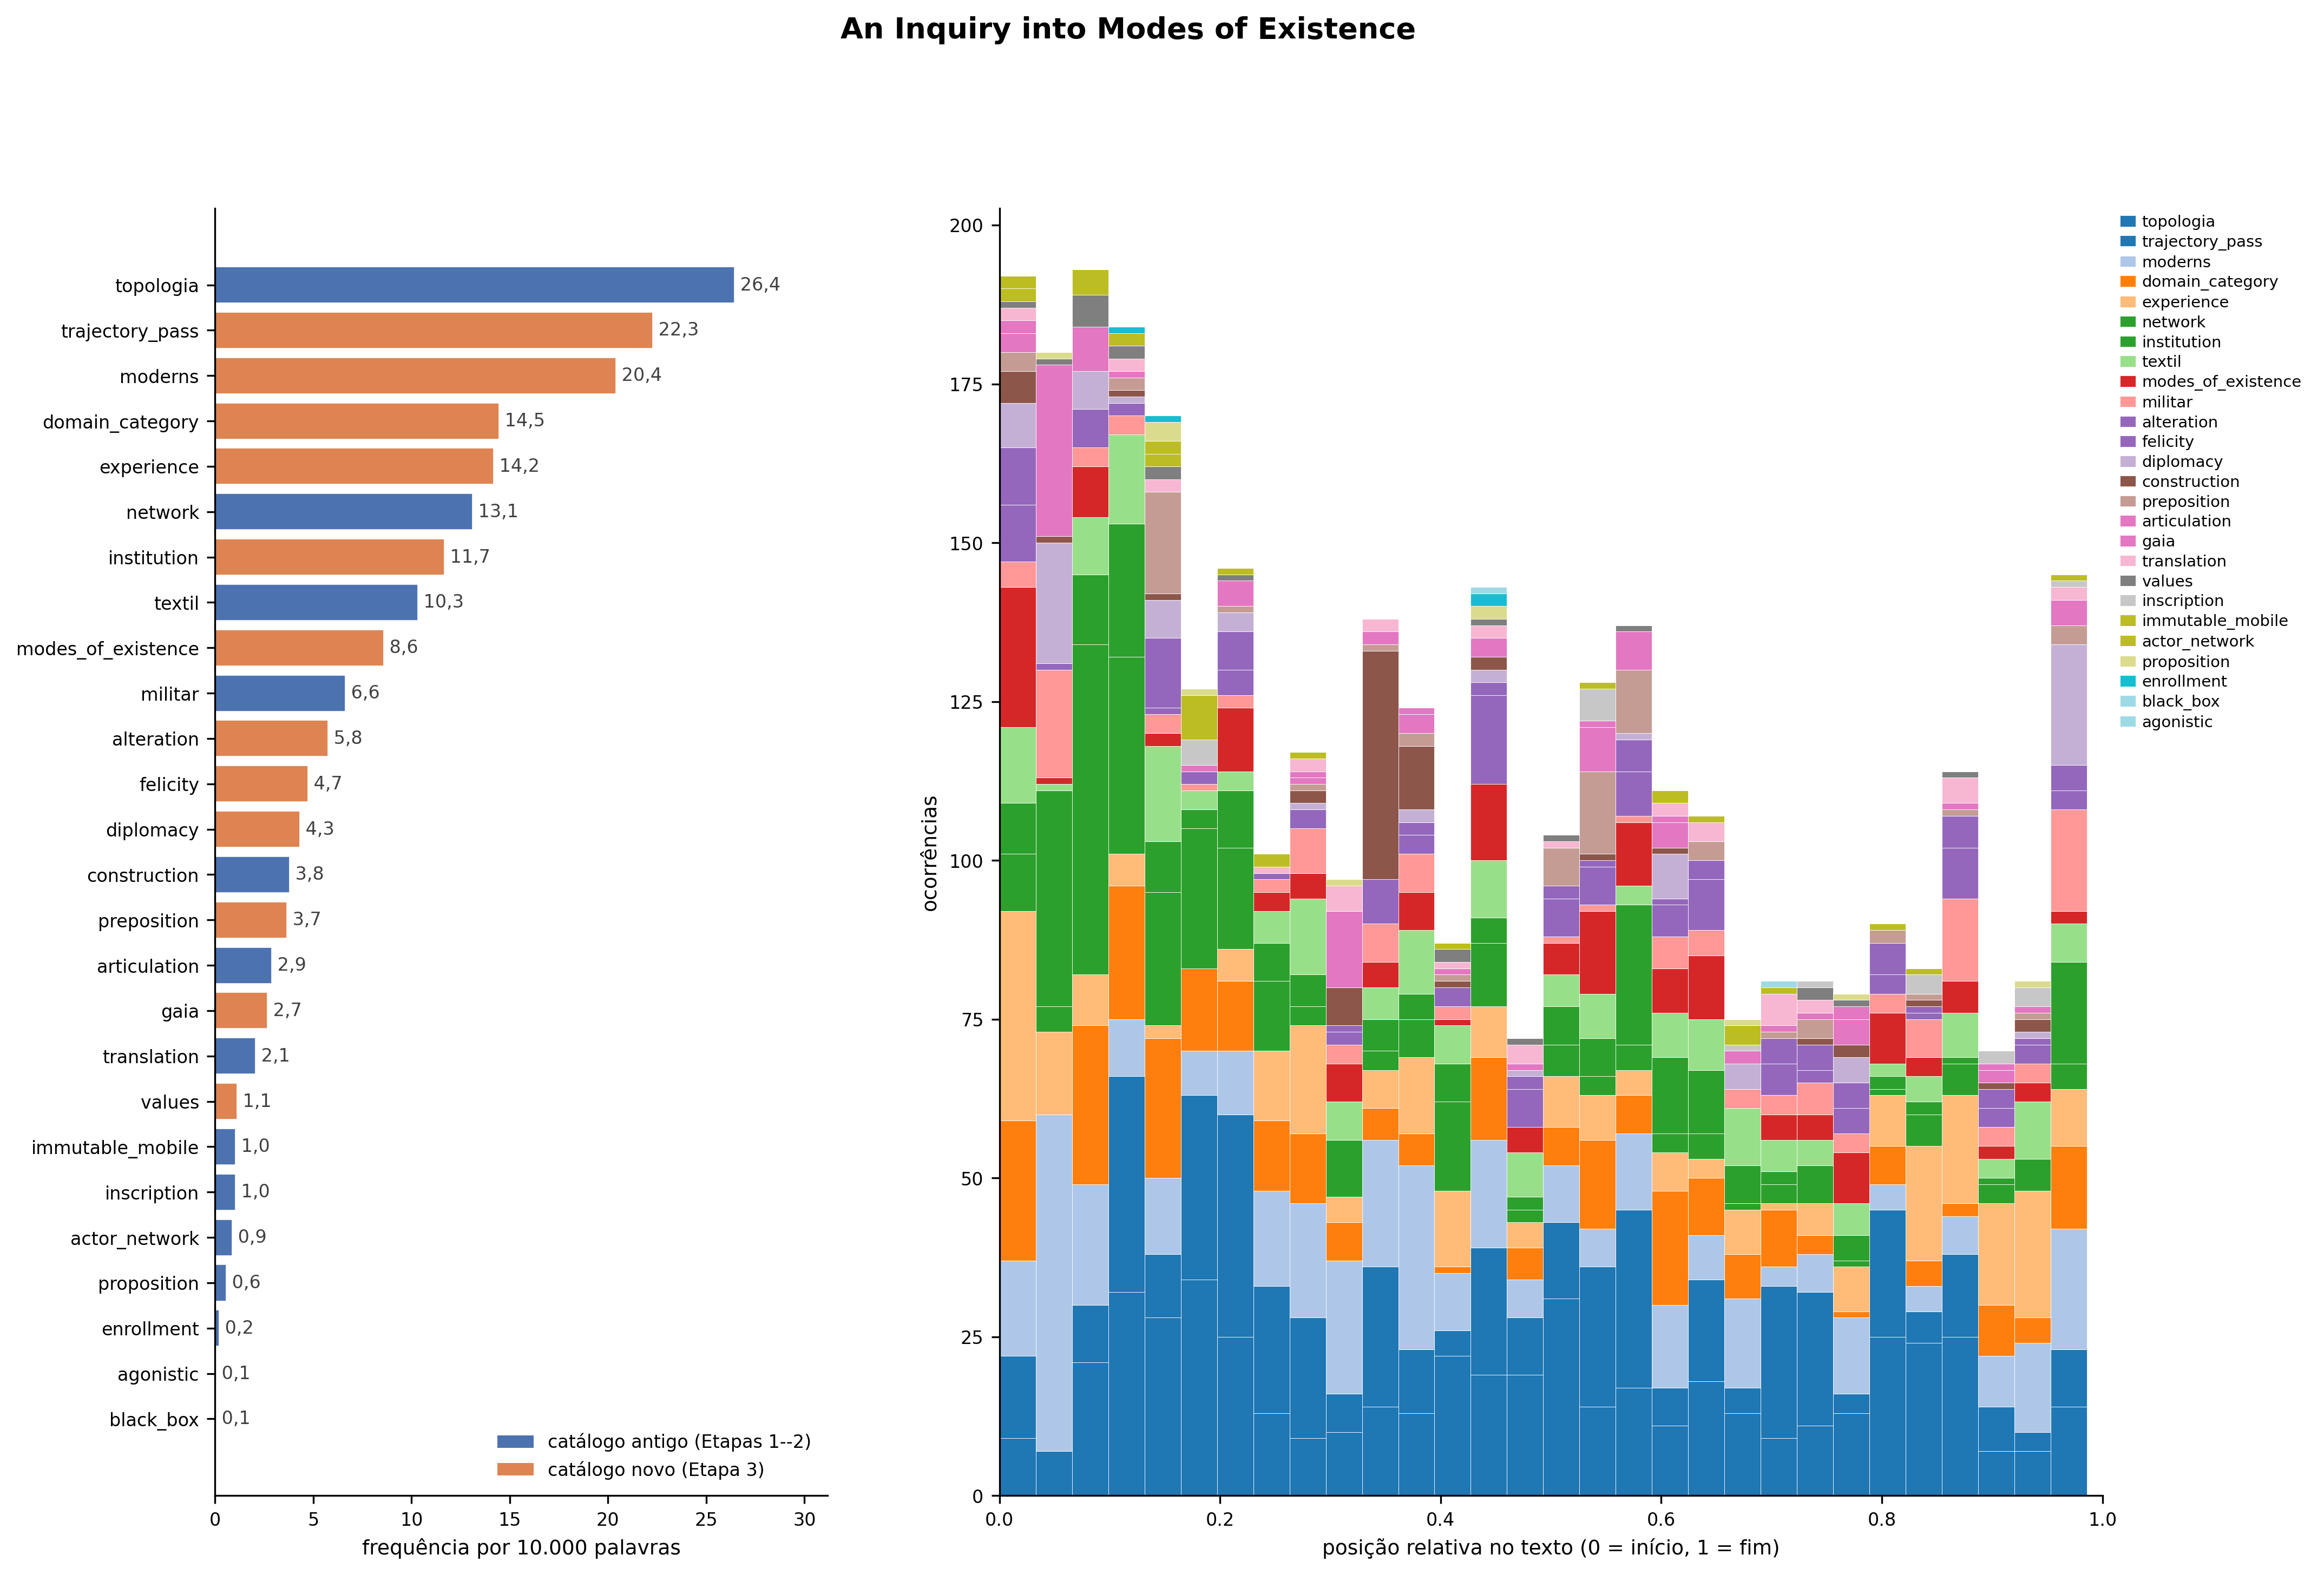
\includegraphics[width=1.0\linewidth]{figuras/cap.2/lexicometria/etapa3_aime_freq_e_densidade.png}
\caption[Frequência e distribuição dos rótulos em AIME]{Frequência e distribuição dos rótulos em \textit{AIME} \parencite{Latour2013Inquiry}. À esquerda, quanto cada um dos vinte e seis rótulos aparece em \textit{AIME}, com duas cores que distinguem o vocabulário figurativo herdado das obras anteriores (em azul) do vocabulário próprio do livro identificado pela leitura qualitativa (em laranja). À direita, onde, ao longo das 194.454 palavras de \textit{AIME}, cada rótulo se concentra ou se distribui, do início ao fim do livro. Soma de 3.557 ocorrências. Os rótulos \texttt{experience} e \texttt{domain\_category} têm alta polissemia em inglês e carregam ruído que a leitura interpretativa precisa considerar. Fonte: análise das figurações em \url{github.com/julianehelanski/analise-figuracoes-latour}.}
\label{fig:aime_freq_densidade}
\end{figure}

A leitura do painel de distribuição registra três regularidades. A primeira: o rótulo \texttt{moderns} aparece em densidade alta e de modo relativamente homogêneo ao longo de todo o livro, em correspondência com a \enquote{antropologia dos modernos} que dá subtítulo à obra. A segunda: \texttt{topologia} e \texttt{trajectory\_pass} concentram densidade alta na primeira metade do livro, na zona dos capítulos introdutórios em que Latour expõe o aparato conceitual dos modos de existência. A terceira: o rótulo \texttt{militar}, décimo na densidade absoluta com 129 ocorrências brutas, distribui-se ao longo do texto sem concentração em capítulo específico, em contraste com o pico inicial que apresentou em \emph{Science in Action} e em \emph{Pandora's Hope}.

O painel registra ainda um movimento de ausência. Cinco rótulos do catálogo antigo zeram em \textit{AIME}: \texttt{centre\_of\_calculation}, \texttt{trial\_of\_strength}, \texttt{factish}, \texttt{circulating\_reference} e \texttt{spokesperson}. Os cinco são neologismos próprios de Latour que ele cunhou ao longo das obras anteriores (\textit{trial of strength} e \textit{centre of calculation} em \emph{Science in Action}; \textit{factish} e \textit{circulating reference} em \emph{Pandora's Hope}; \textit{spokesperson} em \emph{Science in Action}), e o fato de que zeram simultaneamente em livro de 194.454 palavras é dado etnograficamente significativo. O termo \texttt{actor\_network} cai de 24,21 por dez mil em \emph{Clarifications} (1996) para 0,87 em \textit{AIME} (2013), em recuo de mais de vinte e seis vezes. Latour, ao escrever \textit{AIME}, abandona o registro descritivo dos livros e abandona também o vocabulário canônico que ele mesmo cunhou, fazendo com que o \textit{AIME} seja um livro de reformulação sistemática.

A leitura conjunta da tabela~\ref{tab:aime_catalogo_novo} e das figuras anteriores mostra que o vocabulário figurativo herdado das obras anteriores aparece em \textit{AIME} com 1.343 ocorrências distribuídas em dezenove rótulos, ao passo que o vocabulário próprio do livro, aquele que a leitura qualitativa identificou como específico de \textit{AIME}, aparece com 2.214 ocorrências distribuídas em doze rótulos. O vocabulário próprio do livro é, em volume bruto, sessenta e cinco por cento mais denso do que o vocabulário herdado que \textit{AIME} mantém em circulação. A passagem teórica que \textit{AIME} realiza se faz por justaposição entre os dois vocabulários: o livro continua mobilizando o vocabulário da TAR e dos livros monográficos em densidades intermediárias, e acrescenta uma camada figural própria em que predominam \texttt{trajectory\_pass}, \texttt{moderns}, \texttt{domain\_category}, \texttt{experience} e \texttt{institution}. A co-ocorrência entre os rótulos dos dois vocabulários mostra como essa justaposição se organiza: o par mais denso de \textit{AIME}, com 584 co-ocorrências, é \texttt{topologia}--\texttt{trajectory\_pass}, articulação que costura o vocabulário topológico herdado ao vocabulário pragmatista de movimento descontínuo que \textit{AIME} introduz (com variantes \emph{top} \emph{continuity}, \emph{hiatus}, \emph{trajectory} e \emph{discontinuities}).\footnote{Os rótulos \texttt{topologia} e \texttt{trajectory\_pass} compartilham os termos \emph{trajectory} e \emph{trajectories}. Em noventa e cinco posições do texto de \textit{AIME} a mesma ocorrência é contada nos dois rótulos, e essas posições entram como pares de distância nula na contagem de co-ocorrência. A leitura do par como costura entre o vocabulário topológico herdado e o vocabulário pragmatista que \textit{AIME} introduz deve considerar, portanto, que parte da sua densidade decorre dessa partilha de termos, e não apenas da vizinhança textual entre rótulos distintos.} Os pares secundários \texttt{network}--\texttt{topologia} (379 co-ocorrências), \texttt{network}--\texttt{trajectory\_pass} (301), \texttt{domain\_category}--\texttt{topologia} (285) e \texttt{domain\_category}--\texttt{network} (264) sustentam a malha figural integrada do livro.\footnote{A análise de co-ocorrência em \textit{AIME} foi feita em duas configurações de janela de contexto, e o ranking dos dez pares principais se preserva nas duas. A decisão sobre as janelas está documentada em \path{docs/decisoes_metodologicas.md} no repositório público, e a análise é reproduzível pelo procedimento ali versionado.}

O quadro figural de \textit{AIME}, lido nas quatro tabelas e nos pares de co-ocorrência, organiza-se em três camadas. A primeira é a do vocabulário antigo persistente, que \textit{AIME} mantém em densidades intermediárias: \texttt{topologia}, \texttt{network}, \texttt{textil}, \texttt{militar}, \texttt{construction}, \texttt{articulation} e \texttt{translation}. A segunda é a do vocabulário novo pragmatista, próprio do livro, que descreve os modos de existência como tipos de movimento descontínuo qualificados por condições de felicidade próprias: \texttt{trajectory\_pass}, \texttt{experience}, \texttt{alteration}, \texttt{felicity}, \texttt{preposition}, \texttt{modes\_of\_existence} e \texttt{values}. A terceira é a do vocabulário cosmopolítico, em que o livro articula a antropologia dos modernos com a cena diplomática que ele propõe: \texttt{moderns}, \texttt{institution}, \texttt{domain\_category}, \texttt{diplomacy} e \texttt{gaia}. As três camadas se articulam entre si pela co-ocorrência: o vocabulário topológico continuado se costura ao vocabulário pragmatista novo no par \texttt{topologia}--\texttt{trajectory\_pass}, e o vocabulário militar deslocado se costura ao vocabulário cosmopolítico na constelação \texttt{militar}--\texttt{moderns}--\texttt{diplomacy}--\texttt{gaia}.

Explicito o estatuto da análise que apresento nesta subseção, porque ele exige mais cuidado aqui do que em qualquer das obras anteriores. A densidade que registro nas tabelas e nas figuras é medida que se forma no encontro entre o corpus, o catálogo de rótulos que construí para lê-lo e a janela de contexto que defini para contar as ocorrências. Em \textit{AIME} esse encontro tem uma camada a mais, porque a obra é a única do corpus que conto com dois catálogos aplicados em paralelo. A soma de 3.557 ocorrências, e a proporção de sessenta e cinco por cento que separa o volume do catálogo novo do volume do catálogo antigo, são valores que dependem de quantos rótulos compõem cada um dos catálogos e de quais termos reúno em cada rótulo, decisões que tomei na leitura qualitativa de \textit{AIME}. A análise lexicométrica de \textit{AIME} traz ainda uma pendência declarada, uma vez que a desambiguação refinada do rótulo \texttt{militar}, aplicada aos três livros das etapas 1 e 2 e aos dois artigos da etapa 2, não foi aplicada às 129 ocorrências do rótulo \texttt{militar} em \textit{AIME}, e a sua aplicação fica como continuidade do trabalho registrada no repositório. A proporção que leio como o achado central desta subseção sustenta-se enquanto ordem de grandeza, e não como valor exato, pois, o que ela registra que a camada figurativa nova de \textit{AIME} é densa o bastante para rivalizar com a camada herdada, e é dessa forma, o de uma medida co-produzida, que a tomo.

A análise das figurações que sustento neste capítulo~\ref{capitulo2}, organizada pela divisão de trabalho metafórico entre o registro descritivo dos três livros e o registro metateórico dos dois artigos, encontra em \textit{AIME} um terceiro tempo. \textit{AIME} é livro monográfico formalmente, em volume comparável aos livros monográficos solo (194.454 palavras, em ordem de grandeza de \emph{Science in Action} e \emph{Pandora's Hope}), e é livro metateórico em conteúdo, dado que Latour escreve para reformular o vocabulário que ele mesmo cunhou e que orientou cerca de trinta anos de produção. Na análise, identifico que essa posição mista se inscreve no léxico de três maneiras articuladas. A densidade do vocabulário militar em \textit{AIME} é claramente inferior à dos livros, com 6,63 ocorrências por dez mil palavras contra 26,74 em \emph{Science in Action} e 16,56 em \emph{Pandora's Hope}, sem zerar como acontece nos dois artigos. O vocabulário têxtil-topológico permanece em \textit{AIME} em densidade comparável à desses livros, sem o pico que esse vocabulário registra nos artigos. E o vocabulário próprio do livro, aquele que a leitura qualitativa identificou como específico de \textit{AIME}, ocupa o lugar que nas obras anteriores ficava reservado para a descrição da prática tecnocientífica. A guinada das figurações que se desenhava nas obras anteriores, e que esta tese reconstitui através da análise lexicométrica e da leitura situado, fica em \textit{AIME} consolidada como de maneira sistemátia. Latour conserva o vocabulário herdado das obras anteriores, justapõe à elas o vocabulário próprio do livro, e organiza a escrita em três camadas figurativas que articulam a herança da TAR à reformulação dos modos de existência.

A análise das figurações em seis obras de Latour mostra que a tensão entre figuração militar-industrial e figuração têxtil-topológica que organiza esta tese atravessa também a obra latouriana. A figuração militar-industrial, a figuração têxtil-topológica e a figuração cosmopolítico-diplomática coexistem em Latour em densidades que variam por gênero textual, por momento da trajetória e por objeto descrito. Concluo com isso que as três figurações acompanham o movimento de uma escrita que se reescreveu ao longo da produção de Latour, do laboratório de Roger Guillemin em 1979 à investigação sobre os modos de existência dos modernos em 2013.

O repertório que acabo de apresentar não me chegou pronto, e sim por um percurso de leituras que atravessei ao longo da pesquisa, cada uma convocada quando o problema do campo a pediu. Antes de pô-lo em prática no \texttt{C4AI} e no \texttt{Spira}, devo a essas leituras o registro de onde as recolhi e do que cada uma me deu para chegar à inteligência artificial como objeto etnográfico. Refaço a seguir esse percurso, ciente de que reuni-las aqui performa o léxico latouriano do alistamento que a análise das figurações tornou contestável, e mantenho essa consciência ativa como parte do registro reflexivo em que sigo escrevendo.

%%%%%%%%%%%%%%%%%%%%%%%%%%%%%%%%%%%%%%%%%%
\subsection{Costurando figurações: que mundos elas produzem?}
\label{subsec:costurando_figuracoes}

A análise das figurações que apresentei nas seções anteriores me deixou com uma conclusão firme, e é dela que parto aqui: o vocabulário de cada obra de Latour acompanha o objeto que essa obra toma para si. Quando Latour descreve a ciência em ação, o vocabulário que sustenta a descrição é o militar-industrial; quando deixa de descrever a ciência e passa a tecer a própria teoria ator-rede, é o vocabulário têxtil-topológico que ocupa o primeiro plano. A análise mediu esse deslocamento ao longo das seis obras, e a leitura situada mostrou que ele acompanha uma mudança no projeto intelectual de Latour, do laboratório de 1979 à investigação sobre os modos de existência em 2013. Tomo esse achado como premissa, e a pergunta que persigo nesta subseção começa onde ele termina: se a figuração com que se descreve a tecnociência não é neutra diante do que se descreve, que mundos tais figurações faz existir?

A análise lexicométrica indica em que lugar e com que frequência cada figuração aparece, mas não esclarece que mundos elas fazem existir, e é essa segunda pergunta que retomo agora. Uma figuração que explica o funcionamento de uma prática diz, no mesmo movimento, quem faz o quê nessa prática, e por que o faz. A figuração militar de \emph{Science in Action} responde a essas perguntas de um modo determinado: quem faz são os que recrutam aliados, o que fazem é arregimentar reforços e impor provas de força, e o porquê é vencer a controvérsia. A figuração não se restringe, então, a descrever a ciência, porque fornece também o critério pelo qual se separa, nessas práticas, o êxito do fracasso, já que a tecnociência descrita nesses termos funciona bem quando conquista e mal quando é conquistada. Junto com esse critério, a figuração carrega imaginários, teorias e futuros possíveis que modelam tanto as maneiras pelas quais a tecnociência é produzida quanto o modo como pessoas que não são cientistas nem engenheiros a percebem, o que esperam dela e como a utilizam.

E isso não se restringe a imaginários. A figuração com que se descreve uma tecnociência decide, em muitos contextos, quem é protegido e quem é exposto, quem recebe cuidado e quem é deixado sem ele, quem conta como vida que importa e quem é abandonado à conta do dano colateral.\footnote{Uma análise textual que se detém sobre o vocabulário de Latour, de Haraway e de Stengers, que conta figurações e rastreia metáforas, pode parecer afastada desses impactos, mas não é, porque a escolha de uma figuração para a tecnociência tem consequências materiais. O relatório \emph{Artificial Power}, do AI Now Institute, documenta que sistemas de inteligência artificial são levados ao mercado por decisões corporativas antes de adequadamente testados ou validados, e que esses sistemas são empregados em contextos que o próprio relatório nomeia como de vida ou morte, da saúde à defesa, além de serem mobilizados na fiscalização de imigração, em que abusos de direitos humanos são comuns e normas legais são rotineiramente violadas \parencite[pp.~15, 9]{Brennan2025ArtificialPower}. Uma dessas decisões corporativas está registrada na fotografia da figura~\ref{fig:dgx1-openai}, em que o CEO da \texttt{Nvidia} entrega o primeiro supercomputador DGX-1 ao então CEO da \texttt{OpenAI}, Elon Musk, e inaugura a primeira infraestrutura de computação voltada exclusivamente ao treinamento de redes neurais em escala industrial, infraestrutura que mais tarde intensificaria a demanda por energia, água e novos \emph{data centers}. As decisões de cientistas, de engenheiros e, sobretudo, de corporações sobre como descrever, projetar e lançar essas tecnologias não são internas ao laboratório, porque redistribuem proteção e exposição entre populações concretas.} É esse o solo das figurações que mobilizo nesta tese. A inteligência artificial, meu objeto, oferece a esse argumento o seu caso mais agudo. Descrita como inteligência, como nuvem, como sistema imaterial, a inteligência artificial recebe uma figuração que torna invisível a sua base material, e tornar essa base invisível tem consequências sobre a vida humana e não humana. É o que mostra a genealogia material que recuperei no capítulo~\ref{capitulo1} a partir de \textcite{Crawford2021Atlas} que cita como exemplo em como a infraestrutura computacional depende da extração de minérios cujos lucros financiaram décadas de conflito armado com a morte de milhares de pessoas, e cujos custos, o adoecimento e a morte dos mineradores, o capitalismo se sustenta justamente por não contabilizar.% [NOTA DE REVISÃO] verificar/uniformizar a chave Crawford2021Atlas no .bib (a versão antiga da subseção citava Crawford apenas no capítulo 1)

É nesse ponto que a figuração de Haraway faz um movimento de natureza distinta. Haraway não nega que a tecnociência possa funcionar como máquina de guerra. \emph{Ficar com o problema} reconhece, de modo explícito, que os relatos multiespécies que tem por tarefa contar são relatos de uma recuperação em meio a histórias \enquote{tão cheias de morte quanto de vida; tão cheias de finais, e mesmo de genocídios, quanto de inícios} \parencite[p.~25]{Haraway2023Ficar}, e a figura de barbante é apresentada como uma prática situada de \enquote{habitar uma terra vulnerável e ferida} \parencite[p.~25]{Haraway2023Ficar}. A máquina de guerra descreve um modo pelo qual a tecnociência de fato funciona. Todavia, Haraway recusa que esse modo seja o todo da tecnociência e a sua forma necessária. É precisamente porque a máquina de guerra é um modo, e não a totalidade nem o destino da prática, que se abre o espaço para as figurações que faça outra coisa sobre e com a tecnociência. 

A figura de barbante é essa outra figuração, e a diferença está no que ela faz. Haraway a define por dois verbos que não descrevem, e sim fazem: as figuras de barbante \enquote{propõem e põem em jogo padrões para que cada participante possa, de algum modo, habitar uma terra vulnerável e ferida} \parencite[p.~25]{Haraway2023Ficar}. Uma figura que propõe e põe em jogo um padrão apresenta um arranjo possível e o põe em ato, e não se limita a dar conta de como as coisas são. Enquanto o vocabulário militar de Latour explica como a tecnociência funciona, o vocabulário têxtil de Haraway descreve como a tecnociência funciona, com toda a diversidade de objetos, sujeitos, espécies e disciplinas que a compõem, e, no mesmo gesto, propõe como ela poderia funcionar de outro modo. É essa dupla natureza que sustenta o projeto de uma tecnociência situada, responsável e multiespécie, porque descrever a tecnociência pela trama, pelo fio que se passa de mão em mão, é descrevê-la como ela é em parte e, ao mesmo tempo, propor que ela seja tecida de outro modo.

Isabelle Stengers leva esse registro propositivo adiante e o especifica. O que em Latour aparece como o funcionamento da tecnociência, a ciência que vence recrutando aliados e impondo provas de força, Stengers reconhece sob o nome de ciência rápida, a ciência da economia do conhecimento, da pressa e da competição. O gesto de \emph{Uma outra ciência é possível} trata esse modo de funcionamento como um estilo de pensamento particular e seletivo, e não como a ciência em si. A ciência lenta que Stengers propõe não descreve a ciência rápida nem a nega, porque exige dos cientistas que encarem \enquote{o desafio de desenvolver uma percepção coletiva da particularidade e do caráter seletivo de seu próprio estilo de pensamento} \parencite[p.~117]{stengers2018another}. A proposta tem um nome, o \enquote{devir-civilizado}, e uma definição precisa, porque civilizar a ciência é tornar os cientistas capazes de se apresentar a outros coletivos \enquote{de uma maneira que não insulte membros de outros coletivos, isto é, de uma maneira que possibilite um processo de produção de relações} \parencite[p.~117]{stengers2018another}, sem reivindicar um atributo, a objetividade, a racionalidade, que defina o outro como aquele que dele carece. A cosmopolítica que Stengers formula nesse mesmo livro é, na sua própria definição, a recusa de um modo de funcionar, porque \enquote{diz respeito a resistir à tentação de se apressar para concluir} \parencite[p.~167]{stengers2018another} que há uma solução correta capaz de pôr todos os povos de acordo. Leio Stengers e Haraway lado a lado, e a aproximação que proponho entre as duas é minha: tomo a ciência lenta de Stengers como uma figuração que descreve e propõe ao mesmo tempo, no mesmo registro duplo que reconheci na figura de barbante de Haraway, porque ela descreve a tecnociência tal como funciona sob a economia do conhecimento e, no mesmo gesto, propõe que ela seja praticada de outro modo, mais lento, mais atento aos coletivos que a prática acelerada silencia. É a essa leitura que recorro quando digo que Stengers confirma o lado propositivo da figuração têxtil-topológica e lhe dá conteúdo, porque a tecnociência que a figuração de Haraway propõe tecer de outro modo é, no modo como leio Stengers, uma tecnociência desacelerada, que renuncia ao gesto de conquista para tornar-se capaz de fazer relação. % [NOTA DE REVISÃO] páginas de Stengers conferidas pela paginação física do PDF da tradução (Bazar do Tempo, 2023), que suprimiu os fólios impressos: confirmar p.~117 e p.~167 no exemplar físico. Uniformizar a chave: aqui está stengers2018another (minúscula, como na lista de figurações); o .bib precisa de uma só grafia.

A comparação entre as figurações responde, assim, à pergunta que dá título a esta subseção. As figurações produzem mundos diferentes porque fazem coisas diferentes. A figuração militar produz o mundo da ciência como conquista ao torná-lo descritível e ao explicar o seu mecanismo, e o faz no indicativo, como quem constata uma forma de funcionamento. As figurações têxtil-topológicas de Haraway e de Stengers produzem um mundo ao tornar pensável que a tecnociência seja tecida de outro modo, e o fazem em um registro que descreve e propõe ao mesmo tempo. Latour, Haraway e Stengers não se opõem, e a figuração de um não anula a do outro, mas elas diferem no que a figuração faz, porque uma fixa um mecanismo enquanto as outras abrem uma possibilidade. É nesse sentido que escolher uma família de figurações é, ao mesmo tempo, escolher um modo de tornar o mundo descritível e assumir a responsabilidade política pela forma de mundo que esse modo faz aparecer.

A pergunta que essa comparação coloca nesta tese é, dessa maneira, que efeitos reais tem pensar com um tipo de figuração e não com outra? Que modos de pensamento, conhecimento e mundos cada figuração marcada e situada produz quando faço a etnografia da inteligência artificial junto ao \texttt{C4AI} e sobre o \texttt{Spira}, por exemplo? Se não me reconheço fazendo uma revisão bibliográfica no sentido convencional do termo, e se os vocabulários do alistamento e do recrutamento de aliados que herdo junto a figuração militar-industrial que a obra de Latour, que figurações alternativos estão disponíveis, e o que cada um delas produz nesta tese? Não tenho como responder a essas perguntas em definitivo, no entanto, cada figuração produz um conhecimento específico, e o papel de uma etnografia não-inocente está em reconhecer esse repertório de figurações disponível, em utilizá-lo de forma responsável e não-inocente, e em registrar de forma crítica as escolhas de figurações, e outros vocabulários, que cada momento da escrita me exigiu. 

A literatura que adoto nesta tese e neste capítulo~\ref{capitulo1} me oferece um repertório plural, e também desafiador, de figurações que produzem mundos distintos. Apresento-as a seguir, em sequência numerada e em formato que preserva a heterogeneidade de cada uma. O repertório que organizo abaixo é resultado da minha leitura desses autores, e não um inventário de definições que retirei de cada obra. Os princípios, as práticas etnográficas e os vocabulários que reúno em cada linha são a forma como interpreto e aproximo figurações que os próprios autores nem sempre formulam nesses termos, nem sempre articulam entre si, e às vezes sustentam em divergência uns com os outros. Os autores de referência aparecem entre parênteses; o princípio que cada figuração formula vem em primeiro lugar; a prática etnográfica que ela exige vem em segundo; o vocabulário verbal que a figuração mobiliza, em itálico, ao final. Trabalho esse repertório em prática nas seções seguintes deste capítulo~\ref{capitulo2} e nos capítulos~\ref{capitulo3} e~\ref{capitulo4}, e cada figuração reaparece conforme o problema empírico de cada momento da escrita a convoca.

% Requires: \usepackage{array,longtable}
\begin{longtable}{m{3.2cm} m{8.4cm} >{\itshape}m{2.4cm}}
    \caption{Repertório de figurações: o que cada uma formula, a prática que exige e o vocabulário que mobiliza}
    \label{tab:repertorio_figuracoes_cap2} \\
    \hline
    Figuração (autores) & Princípio e prática etnográfica & Verbos \\
    \hline
    \endfirsthead
    \multicolumn{3}{c}{\tablename\ \thetable\ -- continuação} \\
    \hline
    Figuração (autoras) & Princípio e prática etnográfica & Verbos \\
    \hline
    \endhead
    \hline
    \multicolumn{3}{r}{continua na próxima página} \\
    \endfoot
    \hline
    \endlastfoot
    \textbf{Tecitura, costura, \textit{patchwork}, \textit{crazy quilt}} \par (\textcite{Haraway2023Ficar}; \textcite{strathern2011cortando}; \textcite{Law2004After}) & Os fios entram na trama e suas bordas continuam visíveis depois do gesto, e a totalização sob um padrão único é recusada. Descrevo a pesquisa como costura de retalhos heterogêneos e preservo as junções como parte do que se descreve. & costurar, tecer, alinhavar, urdir, atar \\
    \hline
    \textbf{Compostagem} \par (\textcite{Haraway2023Ficar}) & Materiais heterogêneos fermentam ao longo do tempo até se transformarem em matéria nova e fértil, e o humano-como-Homo é recusado em favor do humano-como-húmus. Descrevo a pesquisa como sucessão de fermentações entre materiais antes mantidos separados pelo desenho do método. & compostar, fermentar, decompor-com, adubar \\
    \hline
    \textbf{Figuras de cordas, \textit{string figures},\textit{Science Fiction}} \par (\textcite{Haraway2023Ficar}) & Pensar é trocar padrões com parceiros emaranhados em movimento, e o que importa é o que se passa entre os parceiros, e não o que cada um é. Descrevo a pesquisa como troca de padrões entre humanos e não-humanos em emaranhados simpoiéticos. & jogar com, passar para, receber de, trocar com \\
    \hline
    \textbf{Difração e intra-ação} \par (\textcite{Haraway1997Modest}; \textcite{Barad2007Meeting}) & Os fenômenos produzem padrões de diferença pela interferência mútua, e objeto e instrumento se constituem na relação. Leio um autor através do outro de modo que cada leitura produza diferença nova, e descrevo o campo como configuração intra-ativa. & difratar, intra-agir, interferir-com, fazer-com \\
    \hline
    \textbf{Conexões parciais} \par (\textcite{strathern2005partial}; Haraway) & Entidades se incluem mutuamente sem se reduzir umas às outras, e a totalização é recusada em favor de relações que se sobrepõem. Descrevo as relações entre atores e actantes como conexões que se sobrepõem em recortes específicos. & conectar parcialmente, sobrepor-se a, incluir sem reduzir \\
    \hline
    \textbf{Praxiografia} \par (\textcite{mol2002body}; \textcite{Law2004After}) & Os objetos são múltiplos, feitos diferentemente em diferentes práticas, e a descrição constitui o objeto no ato em que o descreve. Descrevo cada caso etnográfico abarcando a multiplicidade dos objetos. & enactar, performar, fazer-na-prática \\
    \hline
    \textbf{Conversação, oferecimento, hesitação} \par (\textcite{stengers2010cosmopolitics1, stengers2018another}) & A decisão acontece na presença dos que carregarão suas consequências, e a recusa é aceita sem que custe a posição de quem recusa. Ofereço ao leitor o que cada interlocutor disse com suas especificidades históricas declaradas, e recuso o gesto do recrutamento unilateral. & conversar, oferecer, hesitar \\
    \hline
    \textbf{Parentesco, \textit{making kin}} \par (\textcite{Haraway2023Ficar}) & Os parentes não-biológicos são reconhecidos como pertencimento político, e o reconhecimento traz a obrigação de carregar o que o parente carrega. Reconheço responsabilidade pela história política das autoras e dos sistemas técnicos com que trabalho. & aparentar-se, fazer parentes, herdar, carregar-com \\
    \hline
    \textbf{Pensar-com, ficar com o problema} \par (\textcite{Haraway2023Ficar}; \textcite{stengers2018another}) & Pensar é sempre pensar-com humanos, não-humanos, e permanecer com o problema em vez de resolvê-lo prematuramente. Recuso tanto o tecnopositivismo quanto o tecnopessimismo, e permaneço na complexidade sem reduzi-la. & pensar-com, permanecer-com, ficar-com \\
    \hline
    \textbf{Cortar e relacionar} \par (\textcite{strathern2011cortando}; \textcite{Law2004After}; \textcite{Barad2007Meeting}) & A rede só se torna objeto de conhecimento quando interrompida em algum ponto, e o corte produz ao mesmo tempo a rede estendida e o híbrido condensado. Reconheço cada corte etnográfico como decisão analítica situada que produz ao mesmo tempo presença e ausência manifesta. & cortar, recortar, distinguir-com, manifestar-ausência \\
    \hline
    \textbf{Alistar, recrutar aliados} \par (\textcite{Latour2011CienciaEmAcao}; Callon) & A controvérsia se vence alistando aliados que tornam custoso o ataque ao argumento, e a tecnociência funciona como máquina de guerra. Acompanho o alistamento como gesto do campo e reproduzo-o na escrita com a consciência de que essa reprodução é gesto situado. & alistar, recrutar, mobilizar, alinhavar-em-frente \\
    \hline
\end{longtable}

As figurações listadas não constituem uma teoria ou abordagem única, e os autores de referência divergem entre si em pontos significativos. Apesar de identificar esse repertório, não o esgoto por completo. Apresento-o em sua extensão para mostrar o leque de figurações disponíveis e as tensões que o atravessam, e a escolha de quais delas trabalho em cada momento da escrita faz parte de uma decisão situada que tomo capítulo a capítulo, quando oportunas. As divergências entre essas figurações, em particular as que cercam o estatuto do corte, a recusa do corte em favor da continuidade da malha, o gesto da aliança e o registro em que cada autora pratica a sua figuração, já as trabalhei no capítulo~\ref{capitulo1}, onde compus a figuração da costura a partir dessas tensões. Não as retomo aqui. O que importa para o argumento desta seção é que as divergências são parte do que torna o repertório vivo, e que a escolha entre as figurações em cada momento da escrita não é arbitrária, porque cada problema empírico convoca a figuração que melhor permite descrevê-lo, e os capítulos seguintes são um exemplo disso na prática tecnoetnográfica.

A análise das figurações que fiz sobre a obra de Latour, descrita na seção~\ref{sec:analise_lexicometrica} e estendida nas subseções subsequentes, é uma entre as análises textuais que faço nesta tese da minha própria escrita. No capítulo~\ref{capitulo1}, produzi as inscrições tecnocientíficas do meu texto com o \texttt{claude code}, tomando como base uma análise de rede textual dos conceitos ao longo do capítulo, procedimento que repito também ao final dos capítulos~\ref{capitulo2}, \ref{capitulo3} e~\ref{capitulo4}.\footnote{Planejo, depois da defesa, fazer uma análise textual das figurações de todos os capítulos desta tese, para investigar em que medida esse repertório foi de fato praticado, em que distribuição entre os capítulos e com que padrões de co-ocorrência entre as figurações. Como tenho argumentado, as figurações que escolhi utilizar na escrita desta tese são elas mesmas um objeto que se pode descrever, e o repositório \texttt{GitHub} da análise das figurações permanece aberto para essa continuidade.}

Tenho, então, dois movimentos articulados neste capítulo~\ref{capitulo2}. A análise lexicométrica que apresentei nas seções anteriores mediu a insistência de uma figuração na obra de quem mais me serve de fundamentação teórico-metodológica, e me deu a consciência mais crítica sobre com quais tipos de palavras investigo e descrevo a tecnociência. As seções que se seguem percorrem as leituras que atravessei ao longo do doutorado, das quais recolho as interlocuções que cada problema empírico do meu campo provocou. Faço esse revisão bibliográfica já sabendo, pela análise que a antecede, que o gesto de \enquote{convocar} aliados teóricos performa o léxico latouriano que acabei de contestar, mas fico com esse problema na próxima seção.

\section{Estudos da ciência, tecnologia e do digital}
\label{sec:estudos_ciencia_tecnologia}

Começo pelo primeiro grupo das leituras que atravessei, os estudos sociais da ciência e tecnologia e os seus desdobramentos no enfrentamento das tecnologias digitais. Por estudos sociais da ciência e tecnologia entendo o campo que \textcite{Bijker2012Social} ajudaram a fundar ao reunir três abordagens (a construção social da tecnologia, os grandes sistemas técnicos e a teoria ator-rede) sob um princípio comum, o de atentar para o modo como as fronteiras entre o social e o técnico são traçadas pelos próprios atores, em vez de tomá-las como dadas, e descrever ciência e tecnologia como uma teia heterogênea sem costura, em que fatos, artefatos, instituições e interesses se fazem juntos.\footnote{Os editores nomeiam as três abordagens reunidas no volume pelos acrônimos SCOT (\textit{social construction of technology}), LTS (\textit{large-scale technological systems}, de Hughes) e ANT (\textit{actor-network theory}), e identificam como traço comum às três, mais decisivo que as divergências, o princípio metodológico de não assumir de partida a divisão entre o social e o técnico \parencite[pp.~xvi--xvii]{Bijker2012Social}. A \enquote{teia sem costura} (\textit{seamless web}) é a figuração de Hughes para essa indivisão, e a \enquote{engenharia heterogênea} de John Law, autor cujas contribuições aprofundo no capítulo~\ref{capitulo4}, foi reconhecida no \textit{workshop} que deu origem ao livro como expressão afim do mesmo construtivismo.} Uso ao longo desta tese um conjunto de termos que nomeiam o campo e os seus objetos, estudos sociais da ciência e tecnologia, tecnociência, sociotécnico, teoria ator-rede, e, a partir do capítulo~\ref{capitulo3}, tecnopolítica e tecnopoder, e os trato como vocabulário historicamente produzido, em vez de rótulos neutros e intercambiáveis. Cada um se formou em uma tradição e com um propósito particular. Tecnociência vem da filosofia da técnica de Gilbert Hottois, nos anos 1980, e Latour a retoma para nomear a indissociabilidade entre ciência e tecnologia. Sociotécnico nomeia a recusa de separar o social do técnico, princípio que reúne as três abordagens que reuni acima. Teoria ator-rede designa a tradição específica de Latour, Callon e Law, e não o campo inteiro. Tecnopolítica e tecnopoder vêm de uma abordagem crítica das tecnologias digitais, atenta à vigilância, à extração de dados e à concentração de poder, e correm em duas vertentes que mobilizo: a anglófona, ligada aos estudos de mídia e à crítica da indústria de tecnologia, que diagnostica a concentração de poder nas \textit{big techs} \parencite{Kak2023Confronting}, e a latino-americana, situada e decolonial, no registro que redes como a LAVITS sustentam. Ambas carregam uma aposta política que a teoria ator-rede, no seu registro descritivo, não faz. Mantenho essas diferenças ativas porque tomar os termos como equivalentes apagaria as apostas distintas que cada um carrega, no mesmo gesto com que, no capítulo~\ref{capitulo1}, recusei naturalizar o vocabulário herdado. O que une esses termos, por baixo das tradições distintas de que cada um provém, é a forma composta: tecnociência junta ciência e técnica, sociotécnico junta o social e o técnico, tecnopolítica e tecnopoder juntam a técnica e a política, e cada composto recusa, no próprio modo como se escreve, uma das partições que herdamos prontas. É o gesto que defini no capítulo~\ref{capitulo1} a partir de Latour, quando sustentei que a junção dos termos técnica e ciência em \textit{tecnociência} é exigência empírica, e que o campo que eu observava tornava essa exigência particularmente visível.\footnote{Retomo aqui a definição que assentei no capítulo~\ref{capitulo1}, em que descrevo a \textit{tecnociência}, no sentido que \textcite{Latour2011CienciaEmAcao} dá ao termo, como o campo em que ciência e tecnologia se produzem como um só processo, sem partição prévia entre fatos e artefatos, descobertas e invenções, conhecimento e instrumentação. O ponto que retenho para este capítulo é que essa composição não é exclusiva de \textit{tecnociência}, e que \textit{sociotécnico}, \textit{tecnopolítica} e \textit{tecnopoder} repetem, cada um em seu domínio, o mesmo gesto de juntar o que uma divisão herdada mantinha separado, em correspondência com o que a própria teoria ator-rede faz ao recusar tomar como dadas as fronteiras entre o social e o técnico, no princípio que \textcite[pp.~xvi--xvii]{Bijker2012Social} identificam como o traço comum das três abordagens reunidas sob os estudos de ciência e tecnologia.} Tomo esses compostos, portanto, como vocabulário que carrega uma decisão teórica em sua própria forma, e não como rótulos que eu pudesse trocar entre si sem custo. Essa trajetória é sobretudo sociológica, e marco que a antropologia vinha discutindo a técnica e os objetos por uma via própria, de Marcel Mauss e da definição da técnica como \enquote{ato tradicional eficaz} a Lévi-Strauss e ao estatuto teórico que ele deu aos objetos como mediadores de relações, e que dialoga de perto com a filosofia da técnica, de Simondon à cosmotécnica de Yuk Hui que abordei no capítulo~\ref{capitulo1}.\footnote{Essa tradição antropológica da técnica corre em paralelo à genealogia sociológica dos estudos de ciência e tecnologia, e começa nos próprios fundadores da disciplina: Marcel Mauss, \enquote{As técnicas do corpo}, in \textit{Sociologia e antropologia} (São Paulo, Cosac Naify, 2003 [1934]); Claude Lévi-Strauss, \enquote{Introdução à obra de Marcel Mauss}, in Marcel Mauss, \textit{Sociologia e antropologia} (São Paulo, Cosac Naify, 2003 [1950]). A via francesa da tecnologia herda dessa abertura: André Leroi-Gourhan, \textit{O gesto e a palavra} (Lisboa, Edições 70, 1983--1984 [1964--1965]); André-Georges Haudricourt, \textit{La technologie science humaine} (Paris, Éditions de la Maison des sciences de l'homme, 1987). Ela se prolonga no método tecnográfico contemporâneo da cadeia operatória, sistematizado por Pierre Lemonnier, \textit{Elements for an Anthropology of Technology} (Ann Arbor, Museum of Anthropology, University of Michigan, 1992) e \textit{Mundane Objects: Materiality and Non-verbal Communication} (Walnut Creek, Left Coast Press, 2012), e por Ludovic Coupaye, \enquote{Cadeia operatória, transectos e teorias}, in Carlos Emanuel Sautchuk (org.), \textit{Técnica e transformação: perspectivas antropológicas} (Rio de Janeiro, ABA Publicações, 2017, pp.~475--494). Dessa tradição, a interlocução que de fato mobilizo nesta tese vem da filosofia da técnica com que essa antropologia dialoga e tem como referências Gilbert Simondon, \textit{Do modo de existência dos objetos técnicos} (Rio de Janeiro, Contraponto, 2020 [1958]), e Yuk Hui, \textit{Tecnodiversidade} (São Paulo, Ubu, 2020).} Por tecnologias digitais, e pelo digital de modo mais amplo, sigo a orientação não-centrada no digital de \textcite{Pink2016DigitalEthnography}, para quem o digital não constitui uma esfera à parte que se possa isolar e estudar em si, e se descreve melhor como parte do ambiente material, sensorial e social do cotidiano em que pesquiso.\footnote{O princípio do \enquote{não-centramento no digital} (\textit{non-digital-centric-ness}) é um dos cinco que \textcite{Pink2016DigitalEthnography} propõem para a etnografia digital, ao lado de multiplicidade, abertura, reflexividade e o que chamam de \textit{unorthodox}. Tomo-o aqui menos como protocolo metodológico e mais como recorte do objeto, em coerência com a posição que sustento desde o capítulo~\ref{capitulo1}, em que descrevo a inteligência artificial não como esfera técnica isolada, e sim como actante em uma rede sociotécnica heterogênea.} 

Identifico pelo menos quatro temas que organizam a literatura da qual recolho as interlocuções para esta tese, e cada um deles entra quando o problema empírico do meu campo o convocou: a sociologia do conhecimento científico e a virada para a prática, a entrada da tecnologia como objeto de análise por direito próprio, os estudos de laboratório e a teoria ator-rede, e as perspectivas sobre as agências na produção do conhecimento tecnocientífico. Ordeno os quatro pela função que cumprem na minha pesquisa, e não pela cronologia do campo, e tomo como referência para esse recorte o modo como programas de pós-graduação em ciências sociais vêm organizando o ensino do campo. Esta seção não é o registro de uma revisão exaustiva nem de um inventário panorâmico, e sim o registro do que as leituras me deram, de forma direta ou indireta, para chegar ao \texttt{C4AI} e ao \texttt{Spira} como objetos etnográficos aprofundados nos capítulos \ref{capitulo} e \ref{capitulo4}.

O primeiro tema recua à publicação de \textit{A estrutura das revoluções científicas}, de Thomas Kuhn, em 1962, momento em que a ciência deixa de ser tratada como progressão cumulativa de descobertas e passa a ter história, conflitos e paradigmas que rompem com o que veio antes.\footnote{As obras que ancoram este tema são: Trevor Pinch, \enquote{Scientific Controversies}, in James D.~Wright (org.), \textit{International Encyclopedia of the Social and Behavioral Sciences}, 2.~ed., Oxford, Elsevier, 2015, pp.~281--286; Harald Rohracher, \enquote{Science and Technology Studies, History of}, ibidem, pp.~200--205; Steve Woolgar, \enquote{Irony in the Social Study of Science}, in Karin Knorr-Cetina; Michael Mulkay (orgs.), \textit{Science observed: perspectives on the social study of science}, London, Sage, 1983, pp.~239--266; Thomas S.~Kuhn, \textit{The structure of scientific revolutions}, 4.~ed., Chicago, University of Chicago Press, 2012. Para a vertente construtivista e relativista: Barry Barnes; David Bloor; John Henry, \textit{Scientific knowledge: a sociological analysis}, Chicago, University of Chicago Press, 1996; Michael Lynch, \textit{Scientific practice and ordinary action}, Cambridge, Cambridge University Press, 1993; David Bloor, \textit{Conhecimento e imaginário social}, São Paulo, Editora da UNESP, 2009; Harry Collins, \enquote{An Empirical Relativist Programme in the Sociology of Scientific Knowledge}, in Karin Knorr-Cetina; Michael Mulkay (orgs.), \textit{Science observed: perspectives on the social study of science}, London, Sage, 1983, pp.~115--148; Andrew Pickering (org.), \textit{Science as practice and culture}, Chicago, University of Chicago Press, 1992; Steve Woolgar, \textit{Knowledge and reflexivity}, London, Sage, 1988.} A abertura de Kuhn foi adensada pela sociologia do conhecimento científico (\textit{Sociology of Scientific Knowledge}, SSK), que tomou o próprio conteúdo do conhecimento como objeto de explicação social, e se organizou em duas vertentes que dialogam e divergem entre si, o programa forte de David Bloor e Barry Barnes, na Escola de Edimburgo, que postula tratar com os mesmos termos as crenças tidas por verdadeiras e as tidas por falsas, e o programa empírico do relativismo de Harry Collins, na Escola de Bath, que leva a etnografia à bancada para mostrar como as controvérsias se fecham. A partir dessa abertura, uma geração de pesquisadores foi investigar a ciência como prática em disputa, entre eles, Barnes, Knorr-Cetina, Bloor, Collins, Pickering, cada um levando a análise de volta à bancada do laboratório, ao caderno de campo do pesquisador, às reuniões em que fatos se tornam fatos. O programa empírico relativista de Collins demonstrou que o fechamento de controvérsias científicas depende de fatores sociais tanto quanto de evidências, formulação que ecoa quando observo, no \texttt{C4AI}, como os pesquisadores constroem e avaliam seus sistemas de inteligência artificial.

O segundo tema marca a entrada da tecnologia como objeto de análise, e é a partir disso que insiro esta tese nessa literatura. Trevor Pinch e Wiebe Bijker estenderam, em 1984, o argumento construtivista dos fatos científicos para os artefatos, tais como a bicicleta, o bakelite (primeiro plástico sintético) e o microscópio, que resultam de negociações entre grupos sociais com interpretações distintas sobre o que o objeto deve fazer, e a forma estável que assumem é efeito dessas negociações.\footnote{Trevor J.~Pinch; Wiebe E.~Bijker, \enquote{The Social Construction of Facts and Artefacts}, \textit{Social Studies of Science}, v.~14, n.~3, 1984; Steve Woolgar, \enquote{The Turn to Technology in Social Studies of Science}, \textit{Science, Technology, and Human Values}, v.~16, n.~1, 1991; Rachel Laudan, \textit{The nature of technological knowledge}, 2.~ed., Dordrecht, D.~Reidel, 2010; Donald MacKenzie; Judy Wajcman, \enquote{The Social Shaping of Technology}, in MacKenzie; Wajcman (orgs.), \textit{The social shaping of technology}, 2.~ed., Milton Keynes, Open University Press, 1999. A pergunta sobre a política dos artefatos é de Langdon Winner, \enquote{Do Artifacts Have Politics?}, in MacKenzie; Wajcman (orgs.), \textit{The social shaping of technology}, 2.~ed., Milton Keynes, Open University Press, 1999, pp.~26--38, e é retomada criticamente em Langdon Winner, \enquote{Upon Opening the Black Box and Finding It Empty: Social Constructivism and the Philosophy of Technology}, \textit{Science, Technology, and Human Values}, v.~18, n.~3, 1993, pp.~362--378. O exemplo das pontes baixas projetadas por Robert Moses para impedir o tráfego de ônibus em direção às praias de Long Island está no primeiro texto. Registro que esse exemplo foi contestado empiricamente por Bernward Joerges, \enquote{Do Politics Have Artefacts?}, \textit{Social Studies of Science}, v.~29, n.~3, 1999, pp.~411--431, que questiona a evidência histórica da intenção atribuída a Moses e trata a anedota como parábola que circulou no campo mais por sua força retórica que por seu lastro factual. Mantenho o exemplo pela força do argumento que ilustra, a política inscrita na materialidade do artefato, independentemente do que se conclua sobre o caso histórico particular.} A pergunta de Langdon Winner, se os artefatos têm política, tem continuado a inspirar pesquisadores do campo e a manter o problema em aberto. Os exemplos com que esses autores formulam o argumento são conhecidos, uma ponte projetada com altura específica para impedir o acesso de ônibus escolares de minorias pobres a praias, em Winner, e os sistemas técnicos que ordenam decisões sociais sem que sua política apareça, em Pinch, Bijker e na literatura que os segue. A inteligência artificial dá continuidade a esse problema e o intensifica, porque a política deixa de estar inscrita em um artefato isolado e passa a distribuir-se por redes sociotécnicas diversas, dos dados de treinamento aos critérios de otimização e às condições de uso, em que cada nó dessas redes carregam decisões que não se apresentam enquanto tal. O que em Winner era a forma de uma ponte torna-se, na IA, um arranjo de escolhas sociotécnicas dispersas e difíceis localizar e/ou acompanhar, cujos efeitos só se deixam descrever quando se segue a rede inteira que as produz, tarefa que as genealogias críticas do poder tecnológico realizam de forma exemplar e que serão discutidas adiante.

O terceiro tema, ancorado nas etnografias de laboratório, é de onde herdo meu método de base desta tese. Quando Latour e Woolgar entraram no laboratório de Roger Guillemin no Salk Institute, em 1975, realizaram um estudo que viria a se tornar fundador de uma área: tratar a produção de fatos científicos com a mesma seriedade etnográfica com que se acompanhariam práticas em qualquer outro contexto social.\footnote{Bruno Latour; Steve Woolgar, \textit{Laboratory life: The construction of scientific facts}, 2.~ed., Princeton, Princeton University Press, 1986 [tradução: \textit{A vida de laboratório}, Rio de Janeiro, Relume Dumaré, 1997]; Bruno Latour, \textit{Science in action}, Milton Keynes, Open University Press, 1987 [tradução: \textit{Ciência em ação}, 2.~ed., São Paulo, Ed.~Unesp, 2011]; Bruno Latour, \enquote{Give me a Laboratory and I will Raise the World}, in Karin Knorr-Cetina; Michael Mulkay (orgs.), \textit{Science observed: perspectives on the social study of science}, London, Sage, 1983, pp.~141--170.} \textit{A vida de laboratório} é o ponto de partida porque mostra que a tecnociência se faz, que é processo, trabalho e negociação. A teoria ator-rede (TAR) ganha força a partir desse contexto: Michel Callon, estudando as vieiras de St.~Brieuc, e Latour, seguindo Pasteur e seus micróbios, elaboram uma sociologia das associações e das traduções que trata humanos e não humanos sem hierarquias ontológicas e entre o que seria o social e o técnico, e propõe seguir os atores em ação como gesto metodológico que substitui a derivação a partir de estruturas que os precedem.\footnote{Michel Callon, \enquote{Struggles and Negotiations to Define What is Problematic and What is Not}, in K.D.~Knorr; R.~Krohn; R.~Whitley (orgs.), \textit{The Social Process of Scientific Investigation}, Dordrecht, D.~Reidel, 1980; Michel Callon, \enquote{Some Elements of a Sociology of Translation}, in John Law (org.), \textit{Power, action, and belief}, London, Routledge and Kegan Paul, 1986; John Law, \enquote{After ANT: Complexity, naming and topology}, in John Law; John Hassard (orgs.), \textit{Actor Network Theory and After}, Oxford, Blackwell, 1999; Bruno Latour, \textit{Pandora's hope}, Cambridge, MA, Harvard University Press, 1999; Bruno Latour, \textit{Reassembling the social}, Oxford, Oxford University Press, 2005.}

O quarto tema reúne perspectivas sobre as agências na produção do conhecimento tecnocientífico, e é de onde recolho interlocutoras que tensionam as estruturas da TAR. Annemarie Mol, por exemplo, ao estudar a aterosclerose em um hospital holandês, mostrou que a doença é múltipla, feita diferentemente em diferentes práticas, e que essa multiplicidade exige o que ela chamou de \textit{praxiografia} em que o objeto se constitui no ato mesmo da descrição.\footnote{Annemarie Mol, \textit{The body multiple: Ontology in medical practice}, Durham, Duke University Press, 2002. Para outros textos deste tema: Gilead Eyal, \enquote{Spaces between fields}, in Neil Fligstein; Doug McAdam; Neil Gross (orgs.), \textit{Sociological Theory in the Contemporary Era}, Nova York, Norton, 2012; Steven Epstein, \textit{Impure science: AIDS, activism, and the politics of knowledge}, Berkeley, University of California Press, 1996; Donna Haraway, \enquote{Situated Knowledges}, \textit{Feminist Studies}, v.~14, n.~3, 1988; Karin Knorr-Cetina, \textit{Epistemic cultures}, Cambridge, MA, Harvard University Press, 1999; Harry M.~Collins; Robert Evans, \enquote{The Third Wave of Science Studies}, \textit{Social Studies of Science}, v.~32, n.~2, 2002; Sheila Jasanoff, \textit{Designs on Nature}, Princeton, Princeton University Press, 2005.} Donna Haraway, com os conhecimentos situados, recusa a pretensão de um ponto de vista de lugar nenhum e sustenta que todo conhecimento é corporificado, posicionado, parcial \parencite{Haraway1991Situated}. Nas fronteiras contemporâneas do campo, as abordagens materialistas levam adiante o que excede a percepção humana e tensionam as dicotomias natureza-cultura e sujeito-objeto que a teoria ator-rede já começava a deslocar.\footnote{Diana Coole; Samantha Frost (orgs.), \textit{New Materialisms: Ontology, Agency, and Politics}, Durham, Duke University Press, 2010; Karen Barad, \textit{Meeting the Universe Halfway}, Durham, Duke University Press, 2006; Donna J.~Haraway, \textit{The companion species manifesto}, Chicago, Prickly Paradigm Press, 2003; Martin Holbraad, \textit{Can the Thing Speak?}, Open Anthropology Cooperative Press, Working Papers Series 7, 2011; Tim Ingold, \enquote{Materials against materiality}, \textit{Archaeological Dialogues}, v.~14, n.~1, 2007; Bruno Latour, \textit{On the modern cult of the factish gods}, Durham, Duke University Press, 2010 [tradução: \textit{Sobre o culto moderno dos deuses \enquote{fatiches}}, São Paulo, Ed.~Unesp, 2021]. Isabelle Stengers, embora não inscrita na área dos estudos sociais da ciência e tecnologia em sentido disciplinar, mas na filosofia da ciência, atravessa esse quarto tema pela proposta cosmopolítica e pela defesa de uma ciência lenta \parencite{stengers2010cosmopolitics1, stengers2018another}.} Karen Barad, ao propor o realismo agencial a partir da física quântica, faz da intra-ação sua unidade básica de análise, a partir da qual, as entidades não preexistem ao encontro que as constitui, e as relações constituem os próprios termos que as compõem \parencite{Barad2007Meeting}.

Esses quatro temas exemplificam os caminhos abertos pelos estudos de ciência e tecnologia. Em síntese, o primeiro forneceu o aparato para tratar os fatos científicos como construção. O segundo estendeu esse aparato aos objetos e artefatos técnicos. O terceiro mostrou como essa construção acontece na prática. O quarto reformulou a pergunta para examinar quem participa dessa construção, com que agência e em que condições. Dialogo, direta ou indiretamente, com cada um deles. É com a teoria ator-rede, porém, que sigo em grande parte desta etnografia, acompanhando as associações que constroem e sustentam as redes dos pesquisadores que fazem inteligência artificial no \texttt{C4AI}, e adoto, conforme apresentei na seção anterior, o léxico da TAR com a crítica e as figurações que Haraway e Stengers me inspiram a manter ativa.

Os processos e impactos sociais e políticos dos algoritmos e das plataformas digitais, que hoje funcionam quase que totalmente com inteligência artificial, vêm sendo investigados desde a década de 1990, e parte dessa investigação reorganizou os estudos de ciência e tecnologia em dois subcampos: a antropologia digital e a sociologia digital. Foi nas disciplinas de pós-graduação que cursei na \texttt{Unicamp} em 2021, uma de antropologia digital e outra de sociologia da tecnologia, que sistematizei a leitura desses dois subcampos, e é dessa formação que recolho as interlocuções que apresento a seguir.\footnote{A leitura sistemática que apresento nos dois parágrafos seguintes apoia-se no programa e na minha participação em duas disciplinas: \enquote{Antropologia Digital}, ministrada por Carolina Parreiras no Programa de Pós-Graduação em Antropologia Social da \texttt{Unicamp} em 2021, e \enquote{Sociologia da Tecnologia I: vida eletrônica}, ministrada por Pedro Peixoto Ferreira no Programa de Pós-Graduação em Sociologia da \texttt{Unicamp} no mesmo ano. As duas disciplinas não se orientam por autores que escreveram pensando na formação de um campo de estudo unificado, e por isso suas bases são diversas, ainda que compartilhem temáticas e autores comuns.}

A antropologia digital proporciona reflexões teóricas, metodológicas e éticas sobre o avanço das tecnologias de informação e comunicação desde os anos 1990, e examina seus usos, conflitos, formas de regulação, controle, vigilância e desigualdades, em uma abordagem em que a internet é simultaneamente campo, contexto e ferramenta de pesquisa. Os primeiros estudos sobre cibercultura foram feitos por Arturo Escobar, Mike Featherstone e Roger Burrows, Pierre Lévy, Howard Rheingold e, no Brasil, Jean Segata, e a teoria da web foi explorada por Lev Manovich, Nancy Baym e Sherry Turkle.\footnote{Arturo Escobar, \textit{Políticas etnográficas no campo da cibercultura}, Brasília, ABA Publicações, 2016; Mike Featherstone; Roger Burrows, \textit{Cyberspace, cyberbodies, cyberpunk}, London, Sage, 1995; Pierre Lévy, \textit{Cibercultura}, São Paulo, Editora 34, 2005; Howard Rheingold, \textit{A comunidade virtual}, Lisboa, Gradiva, 1996; Jean Segata, \enquote{Um efeito ciber na antropologia}, \textit{Revista Florestan}, n.~4, 2015; Lev Manovich, \textit{The language of new media}, Cambridge, MIT Press, 2000; Nancy Baym, \textit{Personal connections in the digital age}, Cambridge, Polity, 2010; Sherry Turkle, \textit{Life on the screen: identity in the age of the internet}, London, Orion, 1996.} A reflexão metodológica sobre como fazer etnografia em ambientes digitais foi adensada por Daniel Miller e Heather Horst, por Christine Hine, pela \textit{Digital Ethnography} de Sarah Pink, Heather Horst e John Postill que ancora o conceito de tecno-etnografia apresentado no capítulo~\ref{capitulo1}, e, no Brasil, por Carolina Parreiras, Theophilos Rifiotis e o estudo pioneiro de Daniel Miller e Don Slater sobre os \textit{cybercafés} de Trinidad.\footnote{Daniel Miller; Heather Horst, \textit{Digital anthropology}, London, Berg, 2012; Christine Hine, \textit{Ethnography for the internet: embedded, embodied and everyday}, London, Bloomsbury, 2015; Sarah Pink; Heather Horst; John Postill et al., \textit{Digital ethnography: principles and practice}, London, Sage, 2016 \parencite{Pink2016DigitalEthnography}; Carolina Parreiras et al., \enquote{Estratégias para pensar o digital}, \textit{Cadernos de Campo}, v.~29, n.~2, 2020; Theophilos Rifiotis, \enquote{Etnografia no ciberespaço como \enquote{repovoamento} e \enquote{explicação}}, \textit{Revista Brasileira de Ciências Sociais}, v.~31, n.~90, 2016; Daniel Miller; Don Slater, \enquote{Etnografia on e off-line: \textit{cybercafés} em Trinidad}, \textit{Horizontes Antropológicos}, ano 10, n.~21, 2004; Carolina Parreiras, \enquote{Não leve o virtual tão a sério? Uma breve reflexão sobre métodos e convenções na realização de uma etnografia do e no \textit{online}}, in Daniela Moreno Feriani et al. (orgs.), \textit{Etnografias, etnografias: ensaios sobre a diversidade do fazer antropológico}, São Paulo, Annablume, pp.~43--58.} Sobre essa base metodológica a antropologia digital construiu temas próprios, e os que mais ressoam com esta tese são os estudos críticos sobre algoritmos, dados e desigualdades: o trabalho de Tarleton Gillespie e Safiya Noble sobre o poder classificatório dos algoritmos, as questões críticas sobre \textit{big data} formuladas por danah boyd e Kate Crawford, por Cathy O'Neil e por Rob Kitchin, a leitura do colonialismo de dados como acumulação por espoliação proposta por Jim Thatcher, e os estudos sobre desigualdades digitais e sobre a apropriação de \textit{smartphones} e aplicativos no Sul Global.\footnote{Tarleton Gillespie et al., \textit{Media technologies: essays on communication, materiality, and society}, Cambridge, MIT Press, 2014; Safiya Noble, \textit{Algorithms of oppression}, New York, New York University Press, 2018; danah boyd; Kate Crawford, \enquote{Critical questions for big data}, \textit{Information, Communication and Society}, v.~15, n.~5, 2012; Cathy O'Neil, \textit{Weapons of math destruction}, New York, Crown, 2016; Rob Kitchin, \enquote{Big Data, new epistemologies and paradigm shifts}, \textit{Big Data and Society}, v.~1, n.~1, 2014; Jim Thatcher et al., \enquote{Data colonialism through accumulation by dispossession}, \textit{Environment and Planning D}, v.~34, n.~6, 2016; danah boyd, \textit{It's complicated: the social lives of networked teens}, New Haven, Yale University Press, 2014; Paul DiMaggio; Eszter Hargittai, \enquote{From the \enquote{digital divide} to \enquote{digital inequality}}, Working Paper 47, Princeton University, 2001; Massimo Ragnedda; Anna Gladkova (orgs.), \textit{Digital inequalities in the Global South}, Cham, Palgrave Macmillan, 2020; Daniel Miller, \enquote{A theory of a theory of the smartphone}, \textit{International Journal of Cultural Studies}, 2021; Edgar Cruz; Ramaswami Harindranath, \enquote{WhatsApp as \enquote{technology of life}}, \textit{First Monday}, v.~25, n.~12, 2020; Charles Ess; Steven Jones (orgs.), \textit{Readings in virtual research ethics}, Hershey, IGI Global, 2004; Michael Zimmer; Katharina Kinder-Kurlanda (orgs.), \textit{Internet research ethics for the social age}, New York, Peter Lang, 2017.}
Disso distingo uma tradição vizinha, com a qual esta tese também se faz: a antropologia da ciência e da tecnologia, cuja origem está na etnografia das práticas científicas, dos laboratórios e das controvérsias, a linhagem que vai de Latour e da antropologia de Diana Forsythe que retomo no capítulo~\ref{capitulo1}, e não nos estudos de internet e cibercultura de que parte a antropologia digital. No Brasil, essa tradição tem na \texttt{ReACT}, a Rede de Antropologia da Ciência e da Tecnologia, o seu lugar de articulação, e foi em uma de suas reuniões que apresentei parte do que faço nesta tese.\footnote{A primeira Reunião de Antropologia da Ciência e da Tecnologia ocorreu em 2007, e a \texttt{ReACT} consolidou-se como rede em 2013, durante a sua IV Reunião, em Campinas, com gênese, no início dos anos 2000, em um grupo de estudantes de pós-graduação em antropologia. A rede reúne pesquisadores de várias instituições brasileiras em encontros bianuais itinerantes. Participei da IX \texttt{ReACT}, realizada na Universidade Federal de Goiás em novembro de 2023 sob o tema \enquote{ReACTivando o perigo: chamados e ressonâncias frente às crises ecológicas}, onde apresentei trabalho na mesa \enquote{Corpos e Tecnologias}, a primeira vez que a reunião ocorreu fora do eixo sul-sudeste, à exceção de Brasília em 2011. Os anais dessa edição, publicados em 2024, dão a ver as temáticas do grupo, das ecologias multiespécie às ruínas do plantationoceno, com trabalhos sobre inteligência artificial e aprendizado de máquina e uma mesa de homenagem a Bruno Latour, \enquote{Modos de herdar}. A décima reunião ocorreu na Universidade do Estado do Rio de Janeiro em outubro de 2025, ao completar dezoito anos da rede. Disponível em: \url{https://react.labjor.unicamp.br}, \url{https://ocs.ige.unicamp.br/ojs/react} e \url{https://10react.com.br}. Acesso em: 16 jun. 2026.} A rede se constituiu como um gesto a contrapelo do fechamento disciplinar, e a sua apresentação recusa definir o que a antropologia da ciência é para afirmar, em vez disso, aquilo em que ela pode se tornar. Importa-me que ela se descreva com a mesma figuração têxtil que rastreio em Latour ao longo deste capítulo~\ref{capitulo2}: \enquote{aqui, rede é trama e a trama é parte da rede, pois seguem tramando algo sobre si própria e costuram suas alianças}. Em sua décima reunião, a rede sintetizou a proposta atual em torno do que chama de pensar pelo meio: encara de modo simétrico os saberes de dentro e de fora das ciências, mas trata essa simetria como relação entre modos de existência irredutíveis entre si, e não como equivalência, em um gesto que ressoa a ecologia de práticas de Stengers e os conhecimentos situados de Haraway que mobilizo nesta tese.

A sociologia da tecnologia investiga como a vida social é atravessada por tecnologias eletrônicas, e oferece uma análise da vida social mediada por essas tecnologias que se distingue da antropologia digital pela ênfase nas dimensões sistêmicas e materiais. Em torno da expressão \enquote{vida eletrônica}, o subcampo reúne descrições técnicas e investigações críticas sobre as origens, a consolidação e as implicações sociais, econômicas e ambientais dessa realidade, em diálogo com autores como Zygmunt Bauman, Achille Mbembe e Vincenzo Susca.\footnote{Zygmunt Bauman, \textit{Consuming life}, Cambridge, Polity Press, 2007; Achille Mbembe, \textit{Políticas da inimizade}, trad. Sebastião Nascimento, São Paulo, n-1 edições, 2020; Eric Taub, \textit{Does this plug into that? Simplify your electronic life}, Kansas City, Andrews McMeel, 2014; Vincenzo Susca, \textit{Joie tragique: les formes élémentaires de la vie électronique}, Paris, CNRS Éditions, 2010; Vincenzo Susca, \textit{As afinidades conectivas: para compreender a cultura digital}, trad. Simone Cerè, Porto Alegre, Sulina, 2019.} Investigam-se camadas distintas da vida eletrônica. A microeletrônica é a base material que tornou possível a vida eletrônica, e o estudo das primeiras válvulas até a consolidação da microeletrônica a partir dos anos 1950 ancora-se no trabalho de David Brock e Christophe Lécuyer e de Michael Riordan e Lillian Hoddeson.\footnote{David C.~Brock; Christophe Lécuyer, \enquote{Digital foundations: the making of silicon-gate manufacturing technology}, \textit{Technology and Culture}, v.~53, n.~3, 2012; Christophe Lécuyer; David C.~Brock, \textit{Makers of the microchip: a documentary history of Fairchild semiconductor}, Cambridge, MIT Press, 2010; Christophe Lécuyer; David C.~Brock, \enquote{The materiality of microelectronics}, \textit{History and Technology}, v.~22, n.~3, 2006; Michael Riordan; Lillian Hoddeson, \textit{Crystal fire: the birth of the information age}, New York, W.W.~Norton, 2005; Michael Riordan, \enquote{The lost history of the transistor}, \textit{IEEE Spectrum}, v.~41, n.~5, 2004.} A virada cibernética marca a transição para uma compreensão sistêmica da interação entre humanos e máquinas.\footnote{Gregory Bateson, \enquote{Criteria for mental process}, in \textit{Mind and nature: a necessary unity}, New York, E.P.~Dutton, 1979, pp.~89--128; Donna Haraway, \enquote{A cyborg manifesto}, in \textit{Simians, cyborgs, and women: the reinvention of nature}, London, Free Association Books, 1991, pp.~149--181; Norbert Wiener, \enquote{The first and the second industrial revolution}, in \textit{The human use of human beings: cybernetics and society}, Boston, Houghton Mifflin, 1950, pp.~164--189.} A sociologia digital, vizinha próxima da antropologia digital, explora as dimensões sociais e subjetivas das tecnologias, e aborda o ciberespaço, a interação \emph{online} e a subjetividade eletrônica em autores como Sherry Turkle, Fernanda Bruno, Félix Guattari e Michael Heim.\footnote{Sherry Turkle, \textit{Alone together: why we expect more from technology and less from each other}, New York, Basic Books, 2011; Fernanda Bruno, \textit{Máquinas de ver, modos de ser: vigilância, tecnologia e subjetividade}, Porto Alegre, Sulina, 2013; Félix Guattari, \enquote{Da produção de subjetividade}, trad. Suely Rolnik, in André Parente (org.), \textit{Imagem máquina: a era das tecnologias do virtual}, Rio de Janeiro, Editora 34, 1996, pp.~177--191; Michael Heim, \textit{The metaphysics of virtual reality}, New York, Oxford University Press, 1993.} Com temas como o da subjetividade, a sociologia digital examina as dimensões sistêmicas da vida eletrônica, e o conceito de capitalismo eletrônico nomeia o modo como as tecnologias digitais reconfiguraram as estruturas do capitalismo contemporâneo pela automação, pela extração de dados e por formas de exploração mediadas por dispositivos e plataformas, com foco nas questões de vigilância, trabalho digital e mercantilização de dados e comportamentos.

Em meio a essa diversidade de estudos, a inteligência artificial vem ganhando espaço crescente nos estudos de ciência e tecnologia contemporâneos, na antropologia digital e na sociologia digital.\footnote{Na 4S (\textit{Society for Social Studies of Science}), maior evento mundial da área, a ser realizado em Toronto em 2026 sob o tema \textit{Technopolitics}, foram aceitos 244 painéis. Desses, 22 nomeiam inteligência artificial diretamente no título, entre os quais \enquote{The Political Economy Underpinning AI} (Danah Boyd, Janet Vertesi, Alex Taylor e Benjamin Shestakofsky), \enquote{Contesting AI Futures: Grassroots Interventions and Alternative Imaginaries}, \enquote{Polycentric Futures: Governing AI Beyond Monocentric Control} e \enquote{Critical AI Literacy: Power, Governance, and Social Futures}. Quando considero também os resumos, 100 painéis, mais de 40\% do total, abordam inteligência artificial, algoritmos, dados ou plataformas digitais. A programação completa está disponível em: \url{https://www.4sonline.org}. Acesso em: 5 abr.~2026.} Considero a literatura, em especial a brasileira, no movimento de aplicá-la à inteligência artificial como objeto situado, isto é, feita aqui, financiada com recursos públicos e corporativos, atravessada por dependências infraestruturais e por formas de poder que incidem sobre análises próprias. Em como esse movimento está em curso é a proposta, entre outros trabalhos recentes, de \textcite{FazitoCordeiro2026Sociologia} de construir um campo de investigação sociológica sobre inteligência artificial no Brasil a partir da sociologia dos algoritmos.\footnote{Dimitri Fazito; Veridiana Domingos Cordeiro, \enquote{A construção de um campo de investigação sociológica sobre Inteligência Artificial}, Blog da Biblioteca Virtual do Pensamento Social (BVPS), 25 mar.~2026. Disponível em: \url{https://blogbvps.wordpress.com}. Acesso em: 5 abr.~2026.}

\section{Estudos sobre a inteligência artificial e a questão da mediação técnica}
\label{sec:etnografias_ia_mediacao}

% [NOTA DE REVISÃO 1] Parágrafo de abertura da seção revisado. Primeira pessoa ancorada onde estava impessoal: "a segunda parte da seção procura formular" -> "que formulo na segunda parte"; "Convém distinguir os objetos" -> "Distingo os objetos" (regras 7 e 5). Informação editorial retirada do corpo das duas notas e movida para \parencite (regra 5); chave do Collins marcada a conferir. \ref redundante "neste capítulo~\ref{capitulo2}" -> "adiante neste capítulo" (autorreferência). Advérbio "etnograficamente" mantido (permitido pela regra 9; só o verbo é proibido). Argumento e dobradiça epistemológica da nota do Collins preservados integralmente.
Esta seção reúne dois conjuntos de leituras que respondem a uma mesma pergunta por vias distintas: como descrever etnograficamente a inteligência artificial. O primeiro conjunto é o dos precedentes, isto é, as primeiras pesquisas que aplicaram as ferramentas dos estudos de ciência e tecnologia à inteligência artificial como objeto etnográfico, realizadas por Diana Forsythe\footnote{Trabalho publicado postumamente em 2001 \parencite{Forsythe2001}.} na antropologia e por Harry Collins\footnote{Distingo os objetos. \textcite{Collins2012Expert} estudou sistemas especialistas, isto é, programas que codificam o conhecimento de um domínio restrito em regras explícitas do tipo \enquote{se--então}, legíveis e extraídas de um especialista, de comportamento determinístico e auditável, em que a mesma entrada produz sempre a mesma saída e cada decisão pode ser rastreada até a regra que a gerou. Os sistemas de inteligência artificial generativa que descrevo nesta tese são governados por regras de outra ordem, não regras explícitas escritas por programadores, e sim parâmetros estatísticos aprendidos de grandes volumes de dados, de comportamento não determinístico, porque a mesma entrada pode produzir saídas distintas, e de funcionamento interno opaco mesmo para quem os constrói. A pergunta epistemológica de Collins sobre o que é conhecimento e o que pode ser transferido a uma máquina sobrevive a essa mudança de arquitetura, ainda que o objeto a que ela se aplica tenha mudado de natureza, e é essa diferença que formulo na segunda parte da seção.} na sociologia. O segundo conjunto é o da contribuição teórica que desenvolvo a partir do conceito de \textit{mediação técnica}, e que me ajuda a formular um quadro para descrever o que muda quando a inteligência artificial passa a gerar textos, imagens e sons, e, pela primeira vez na história da computação, de forma não determinística. Ligo os dois conjuntos porque Forsythe e Collins estudaram a inteligência artificial simbólica e os sistemas especialistas das décadas de 1980 e 1990, e a contribuição teórica que apresento na segunda parte da seção retoma a pergunta deles para os sistemas de inteligência artificial generativa contemporâneos. O campo brasileiro sobre IA nas ciências humanas é emergente, como documenta a análise bibliométrica que apresento adiante neste capítulo, e esses precedentes internacionais situam o tema em uma linhagem que já existe há quatro décadas, ainda que tardiamente recebida no Brasil.

\subsection{Antropologia da inteligência artificial: Diana Forsythe}

\epigrafe{%
Much of what they actually do in the Lab is thereby rendered invisible, relegated to a category of unimportant or illegitimate work. Among these deleted activities are the many acts of social, in tellectual, and material maintenance that lie outside the realm of formal problem-solving. This systematic deletion is taken for granted in the world of expert systems: in anthropological terms, it is part of the local culture.}%
{Diana Forsythe, \textit{Studying Those Who Study Us: An Anthropologist in the World of Artificial Intelligence}, 2001, pp.~29-30}

Diana E.~Forsythe (1947--1997) está entre as primeiras pesquisadoras a realizar etnografia em laboratórios de inteligência artificial. O conjunto de seu trabalho \parencite{Forsythe2001}\footnote{Esta obra é compilação de ensaios e reflexões que resgatam textos finais e inéditos de Forsythe, organizada por David J.~Hess. O volume analisa as culturas disciplinares da inteligência artificial e da informática médica, com base no trabalho de campo etnográfico que a autora realizou em laboratórios de IA.} oferece análise da cultura da inteligência artificial com foco no subcampo da informática médica e no desenvolvimento de sistemas especialistas baseados em conhecimento. Esses sistemas, que codificavam o conhecimento de um domínio restrito em regras explícitas para emular o raciocínio de um especialista humano, eram a forma dominante da inteligência artificial nas décadas de 1980 e 1990, a inteligência artificial simbólica anterior à virada para o aprendizado de máquina e o aprendizado profundo. O que Forsythe estudou, portanto, foi a IA tal como ela existia em seu tempo, e essa distinção importa para o que proponho adiante, quando estendo o argumento dela aos sistemas de inteligência artificial generativa, de arquitetura técnica muito diferente.

O estudo de Forsythe foi moldado por sua história pessoal. Seu pai, George Forsythe, foi o presidente fundador do departamento de ciência da computação da Universidade Stanford, e sua mãe, Alexandra Forsythe, foi uma referência no ensino de ciência da computação e enfrentou discriminação de gênero ao longo da carreira. A trajetória profissional de Forsythe deslocou-se dos estudos europeus para a antropologia da tecnociência em 1985, e em seguida ela passou aproximadamente oito anos como participante-observadora em tempo integral em cinco laboratórios de sistemas especialistas, quatro em ambientes acadêmicos e um na indústria.

O argumento de Forsythe é que os profissionais de IA, ainda que vejam seu trabalho como objetivo e culturalmente neutro, trabalham dentro de uma cultura disciplinar que modela como definem problemas, o que consideram conhecimento, como realizam seu trabalho e os limites dos sistemas que constroem. Para descrever a tendência dessa cultura a ignorar e tornar invisíveis dimensões sociais, contextuais e informais da realidade, ela toma emprestado da socióloga Susan Leigh Star o termo \enquote{eliminação do social} (\textit{deletion of the social}). Forsythe observou disparidade sistemática entre o que profissionais de IA dizem que fazem e o que fazem quando observados: eles descrevem seu trabalho como composto por algumas tarefas técnicas, conceituar e resolver problemas, escrever código e construir sistemas, e classificam como \enquote{pseudo-trabalho} (\textit{pseudo-work}) grande parte de suas atividades diárias, como reuniões, correspondência eletrônica, recrutamento e busca de financiamento.\footnote{A distinção entre \enquote{trabalho real} (\textit{real work}) e \enquote{pseudo-trabalho} é registrada por Forsythe a partir das próprias palavras de seus interlocutores, que separavam o \enquote{trabalho real} ou \enquote{IA real}, isto é, a conceitualização, a escrita de código e a construção de sistemas, do \enquote{resto} que precisavam fazer. Quando perguntados sobre em que consistia seu trabalho, descreviam apenas o primeiro \parencite{Forsythe2001}.} O ponto decisivo do argumento é o paralelo entre dois gestos. Essa mesma noção formal e descontextualizada de trabalho, que os engenheiros aplicam a si próprios, é a que eles projetam sobre os especialistas cujo conhecimento tentam capturar: a elicitação do conhecimento concentra-se em tarefas formais e isoladas, observadas fora do contexto de trabalho, e deixa de fora os processos informais, sociais e institucionais que são parte constitutiva do desempenho dos especialistas em situação. Daí resultam sistemas que a literatura técnica designa por \textit{narrow} e \textit{brittle}: o conhecimento codificado é estreito porque deixa muito de fora, e frágil porque carece de informação sobre os contextos que dão sentido aos modelos e sobre como esses modelos se traduzem em ação na vida real, de modo que os sistemas funcionam dentro dos domínios para os quais foram programados e colapsam diante de situações que seus construtores não anteciparam.

Em um de seus ensaios, Forsythe voltou-se para a invisibilidade das mulheres na cultura da pesquisa em inteligência artificial. Como a maior parte das mulheres nos laboratórios ocupava funções administrativas ou de apoio, seu trabalho não contava como trabalho técnico, e afirmações como \enquote{não há mulheres no laboratório} eram frequentes mesmo diante de trabalhadoras presentes.\footnote{Diana E.~Forsythe, \enquote{Disappearing Women in the Social World of Computing}, in \textit{Studying Those Who Study Us: An Anthropologist in the World of Artificial Intelligence}, Stanford, Stanford University Press, 2001. Forsythe constatou que a invisibilização funcionava em vários níveis, desde a escassez de mulheres na área até o não reconhecimento do trabalho que elas de fato realizavam. Esse tipo de invisibilização, somado à hierarquia de poder generificada na ciência da computação, acabava por pressionar as mulheres a aderir ao silêncio ou a deixar a área. A análise tem ressonância biográfica: o pai de Forsythe tornou-se um cientista da computação reconhecido, ao passo que sua mãe, também cientista, foi marginalizada na carreira, episódio que retomei na subseção anterior.} Esse apagamento que Forsythe observou nos laboratórios dos anos 1990 tem uma história mais longa, que volta às origens do próprio trabalho computacional, e da qual discuto alguns aspectos no capítulo~\ref{capitulo3}, ao seguir a \texttt{IBM} até a sua origem nas máquinas de tabulação de Herman Hollerith.\footnote{No capítulo~\ref{capitulo3} acompanho essa trajetória paradoxal, da abertura do trabalho de escritório às mulheres com a máquina de escrever e da predominância feminina na computação realizada por humanos e na programação até a masculinização da área a partir dos anos 1960--1970, com base em \textcite{Light1999When}, \textcite{Ensmenger2010Computer} e \textcite{Abbate2012Recoding}, e analiso o caso das operadoras das máquinas de Hollerith no Censo estadunidense de 1890 como momento de transição desse ciclo.} No entanto, no campo de Forsythe, nos anos 1980 e 1990, essa composição não era reconhecida como problema pelos próprios pesquisadores, e coube a ela, como antropóloga, torná-la visível pela etnografia, evidenciando como a cultura do laboratório fazia as mulheres desaparecerem mesmo quando presentes. No meu campo, eu também observei desde cedo uma composição majoritariamente masculina e branca, que anotei no caderno e que percebo agora como eco do estudo de Forsythe.\footnote{Caderno de campo, 19 de outubro de 2022. Registro aqui uma observação sobre o estatuto das falas que reconstituo a partir do caderno nesta e nas próximas páginas. Como as anotações foram feitas no decorrer dos eventos, nem sempre pude transcrever ao pé da letra o que foi dito, e boa parte do material foi reescrita de memória logo depois. Por isso reservo as aspas para as poucas expressões que anotei como fórmulas no momento da fala, e mantenho em discurso indireto o que reconstituí, sinalizando a diferença entre transcrição e reconstrução pela memória.} O incômodo foi meu no começo, mas decidi deixar que o próprio campo me mostrasse se aquilo representava um problema para os pesquisadores.\footnote{Devo este deslocamento, entre tantos outros, a Suely Kofes, minha orientadora, que na leitura do meu texto de qualificação chamou minha atenção para o tratamento da questão do gênero. Na primeira versão da tese, eu havia feito juízo precipitado sobre a composição de gênero do Centro, e julgava também a partir de quem eu era naquele momento, uma mulher e uma pessoa de fora da ciência e da engenharia da computação. O que aprendi com ela vem também de uma leitura de \textcite{strathern2014efeito}: \enquote{homem}, \enquote{mulher} e \enquote{gênero} não são categorias dadas que eu pudesse aplicar de fora ao campo, e sim categorias que se constituem nas próprias relações. Assim, deixei que os actantes falassem, por mais difícil que isso seja, e de acordo com \textcite{Latour1999RecallingANT}.}

Diferentemente dos laboratórios e da época de Forsythe, no \texttt{C4AI} a composição de gênero não era questão tácita, mas problematizada pelos próprios pesquisadores. Acompanhei isso primeiro em campo, no evento de apresentação do Centro, antes de reencontrá-lo nos relatórios anuais enviados à \texttt{FAPESP}. Na abertura, la diretora do Comitê de Inclusão e Diversidade trouxe à tona o problema: disse que o Centro era, em sua maioria, dos pesquisadores aos cargos de hierarquia superior, composto por \enquote{homens brancos}, e marcou ela mesma a pergunta sobre onde estavam as mulheres.\footnote{Caderno de campo, 19 de outubro de 2022. A fala da diretora durante o evento está documentado nos relatórios anuais. O censo interno realizado em julho de 2021 encontrou 37\% de homens brancos, 31,5\% de mulheres brancas, 13,7\% de homens pardos, 8,2\% de mulheres pardas e 9,6\% de outros grupos, e o relatório registra que, naquele momento, todos os investigadores principais (\textit{principal investigators}) do Centro eram homens cis brancos, a maior parte das mulheres eram estudantes, e não havia pessoas pretas, pessoas com deficiência nem transgênero \parencite[os relatórios estão em inglês, tradução minha]{C4AI2021}. O relatório seguinte acrescenta que, depois disso, o conjunto de investigadores principais se diversificou com a inclusão de Lucia Santaella, Cristina Godoy Bernardo de Oliveira e Sandra Aluísio \parencite{C4AI2022}.}

Os cinco relatórios\footnote{Tive acesso aos cinco relatórios anuais por uma cadeia de mediações que é, ela própria, dado importante no meu campo. Durante a entrevista que realizei com Cláudio Pinhanez, vice-diretor do Centro, em outubro de 2025, conversamos sobre as pesquisas do \texttt{C4AI} e manifestei meu interesse pelos dados de publicações do Centro; ele me orientou a solicitá-los a Fábio Cozman, diretor, que me deu acesso aos relatórios e autorizou seu uso para fins desta pesquisa.} anuais entregues à \texttt{FAPESP} entre 2021 e 2025 documentam que o Comitê Executivo do \texttt{C4AI} foi composto pelas mesmas quatro posições em todos os cinco anos, ocupadas pelo diretor Fabio Gagliardi Cozman, pelo vice-diretor Claudio Pinhanez, pelo coordenador de Difusão Fernando Osório e pelo coordenador de transferência de tecnologia Glauco Arbix, com a presença do gerente executivo Jairo Carlos Filho \parencite{C4AI2021, C4AI2022, C4AI2023, C4AI2024, C4AI2025}.\footnote{Os relatórios nomeiam os ocupantes e seus cargos, e não descrevem sua identidade de gênero; identifico-os como homens a partir dos nomes, pronomes e presença pública com que comparecem no campo, e não atribuo a eles a categoria \enquote{cis}, que o Centro emprega em outro contexto, o do censo, como autodescrição de seus \textit{principal investigators}. O relatório de 2021 registra ainda Eliana Futenma como assistente administrativa do Comitê, função de apoio ocupada por uma mulher.} Na camada imediatamente abaixo, a liderança nominal dos grupos de pesquisa, em 2021 havia duas mulheres entre os doze líderes dos cinco desafios de pesquisa, Sandra Aluísio no processamento de linguagem natural para o português e Cristina Godoy Bernardo de Oliveira em \textit{AI-Humanities}. Em 2025, após a reorganização dos grupos, havia quatro mulheres na liderança, Sandra Aluísio no processamento de linguagem natural, Luciana Storto nas línguas indígenas, Sarajane Marques Peres em \textit{Knowledge-Enhanced Machine Learning} e Cristina Godoy Bernardo de Oliveira no Observatório Brasileiro de Inteligência Artificial (OBIA), concentradas em processamento de linguagem natural, línguas indígenas, conhecimento e impacto social, e ausentes dos grupos de aprendizado de máquina aplicado a oceanografia, clima e diagnóstico médico.\parencite{C4AI2021, C4AI2025}.\footnote{O relatório de 2022 registra que a inserção de Lucia Santaella, Cristina Godoy Bernardo de Oliveira e Sandra Aluísio como investigadoras principais no sistema SAGE da \texttt{FAPESP}, posterior ao censo de julho de 2021, foi apresentada como diversificação da equipe \parencite{C4AI2022}. Sandra Aluísio e Cristina Godoy, porém, já lideravam desafios de pesquisa em 2021, de modo que essa diversificação foi, em parte, regularização administrativa retrospectiva de uma presença que já estava em curso.}

O trabalho de inclusão efetivamente exercido pelo Centro concentrou-se no programa de bolsas gerido pelo Comitê de Inclusão e Diversidade, formado em abril de 2021 sob a liderança de Renata Wassermann e Valdinei Freire e voltado a estudantes de graduação da \texttt{USP} de grupos sub-representados. O processo seletivo, que a diretora descreveu na mesma fala do evento, partiu de mais de trezentas candidaturas para poucas vagas, e ela registrou a dificuldade de selecionar entre tantas pessoas interessadas.\footnote{Os relatórios precisam esses números: ao primeiro edital, de setembro de 2021, candidataram-se mais de trezentas pessoas, das quais o Comitê selecionou vinte e quatro para uma segunda rodada, com envio de um vídeo de três minutos, antes de definir a turma final \parencite{C4AI2022}. As turmas reuniam doze bolsistas, com maioria de mulheres cis, de pessoas negras e de estudantes de escola pública, além de pessoas com deficiência e, na turma de 2023, uma pessoa transgênero, e a maioria com renda familiar de até quatro salários mínimos \parencite{C4AI2022, C4AI2023}.} O programa recebeu o Selo de Direitos Humanos e Diversidade da cidade de São Paulo, anunciado em outubro de 2023.\footnote{O relatório de 2022 registrava que o programa concorria ao Selo, e o de 2023 confirma a premiação \parencite{C4AI2022, C4AI2023}.}

Na mesma cerimônia, o representante da \texttt{IBM} deu ênfase ao Comitê, pediu uma salva de palmas e que os bolsistas presentes levantassem a mão, e declarou que a iniciativa partira da empresa, tendo em vista o compromisso da \texttt{USP} com a diversidade e as expectativas de negócios diante dos resultados sociais positivos da inclusão de maior diversidade de pessoas nas empresas. A diversidade comparecia, ali, em dupla inscrição, por um lado, como demanda institucional da Universidade, e por outro, como valor de negócio para a corporação que financiava o Centro, articulação que retomo no capítulo~\ref{capitulo3}.

Fábio, em muitas de suas falas públicas, destacava o trabalho do Comitê como um \enquote{diferencial} do \texttt{C4AI}. Participei de algumas reuniões do grupo, junto aos professores coordenadores e aos pesquisadores que ingressaram por um edital específico, e além da diversidade de gênero foram contempladas diversidades étnico-raciais, de idade e de áreas do conhecimento. Mais do que contabilizar essa diversidade, o Comitê funcionava como espaço de inserção dos estudantes no mundo da ciência da computação e da inteligência artificial, por meio de bolsas de iniciação científica específicas, estudantes de grupos sub-representados eram introduzidos nessas áreas e encaminhados para dar continuidade às pesquisas no mestrado e no doutorado.\footnote{O programa foi reestruturado no primeiro semestre de 2024 e a nova turma, mais enxuta, começou em fevereiro de 2025. O Centro justificou a redução pelo fato de que \enquote{a Universidade como um todo tem agora um foco muito mais forte em inclusão por meio de um amplo conjunto de programas} \parencite[tradução minha]{C4AI2025}.} Foi por esse eixo, e pela colaboração com o grupo \textit{AI-Humanities}, que depois se tornou o Observatório Brasileiro de Inteligência Artificial, que ingressei no Centro, e é como colaboradora desse grupo, e não dos grupos técnicos, que apareço nominalmente nos relatórios institucionais a partir de 2023.\footnote{O relatório de 2023 me registra de duas formas, na mesma página: como uma das responsáveis pelas aulas mais específicas da formação dos bolsistas, ao lado de \enquote{\textit{Thiago Marcílio, Juliane Cristina Helanski Cardoso}}, e como pesquisadora visitante recebida pelo Comitê no primeiro semestre de 2023, ao lado de Mayane Batista Lima, doutoranda em Antropologia Social pela UFAM, ambas trabalhando com a turma de bolsistas daquele ano \parencite[p.~27]{C4AI2023}. No relato sobre as visitantes sou descrita corretamente como doutoranda em ciências sociais na \texttt{Unicamp}, mas na lista de membros do grupo, no mesmo relatório, apareço como \enquote{\textit{Doctoral student in Anthropology at \texttt{Unicamp}, developing an ethnographic study of Artificial Intelligence researchers}}, descrição que o relatório de 2025 repete \parencite[p.~27]{C4AI2023, C4AI2025}.}

Não cheguei a essa questão de imediato. Ela emergiu quando pedi ao \texttt{claude}, no trabalho de revisão que descrevo neste capítulo~\ref{capitulo2}, que comparasse as minhas anotações do caderno de campo sobre o Comitê de Inclusão e Diversidade com os cinco relatórios anuais, para verificar se os números que eu havia registrado batiam com o que os documentos diziam, e vice-versa, pois já fazia algum tempo que eu não visitava esses documentos com esse propósito. Esse cruzamento, que fiz em conjunto com o \texttt{claude}, reavivou uma tensão de uma das aulas que ministrei na formação dos bolsistas, atividade pela qual apareço nos relatórios sem que eu, no momento em que a vivi, me reconhecesse fazendo parte daquela formação. Eu havia apresentado \textcite{pasquinelli2020nooscópio} e \textcite{Crawford2018Anatomy} como referências, e os professores da área responsáveis pelo grupo questionaram o modo como esses autores definiam conceitos da ciência da computação, entre eles o de algoritmo, discordaram em vários aspectos e consideraram simplificante demais a posição que eu trazia. Dar uma aula sobre algoritmo para cientistas da computação, como cientista social e a partir de autores críticos, foi uma experiência desafiadora, e talvez a escolha do tema não tenha sido a mais feliz, mas quis pôr lado a lado as duas leituras justamente porque, como discuto no capítulo~\ref{capitulo1}, o social também é com frequência tomado como dado e simplificado pelos pesquisadores de IA. Foi uma tentativa de começar um diálogo e de construir o que \textcite{stengers2010cosmopolitics1} chama de alianças, e a discordância que daí saiu, embora não fosse a concordância que eu buscava, talvez já fosse a aliança no sentido de Stengers, que não se reduz ao consenso nem à mera convivência cordial entre posições, e sim nomeia a composição entre práticas que não se submetem a um critério comum, criando a possibilidade de consistência onde antes havia só confrontação \parencite[][p.~vii]{stengers2010cosmopolitics1}.\footnote{Stengers formula a aliança no registro da \textit{ecologia das práticas} que organiza os dois volumes de \textit{Cosmopolitics}. A coexistência entre saberes heterogêneos, como o neutrino da física e os múltiplos mundos mobilizados pela etnopsiquiatria, tem sentido sem que nenhum corpo unificado de conhecimento demonstre que eles podem coexistir, e esse sentido, escreve ela, não tem nada a ver com tolerância nem com ceticismo desencantado \parencite[p.~vii]{stengers2010cosmopolitics1}. A aliança, nesse sentido, não dissolve a diferença entre as práticas que a compõem, e é por isso que a discordância pode ser sua forma, e não seu fracasso. Essa leitura ressoa com a recusa do confronto estéril e a defesa do diálogo difícil entre coabitantes que \textcite[p.~314]{costa2024manchando} desenvolve a partir de Stengers.} Foi nesse cruzamento, posto em relação com a leitura de Forsythe e a questão de gênero que ela levanta, que reli o material e vi a minha própria inscrição nos documentos: eu já sabia que era citada no relatório como \enquote{colaboradora individual}, mas o cruzamento deu a ver que eu também era mencionada dentro daquele grupo, e em dupla posição, como quem ministrava parte da formação dos bolsistas e como pesquisadora visitante que observava essa mesma formação. O episódio é, ele próprio, o que \textcite{strathern2014efeito} chama de efeito etnográfico, isto é, aquilo que se produz quando observação e análise são postas em relação no momento da escrita, prática autoconsciente em que um segundo campo se cria e devolve o que o primeiro não dava a ver.\footnote{Para Strathern, o trabalho de campo guarda uma relação complexa entre dois campos, o etnográfico e o teórico, que se tocam sem se sobrepor, e o efeito etnográfico não preexiste à escrita, e sim se produz nela, no momento em que observação e análise entram em relação. A escrita etnográfica é, nesse sentido, prática autoconsciente sobre a própria autoria, e não transcrição de um campo já dado \parencite{strathern2014efeito}.}

Este momento se tece com vários fios que venho (des)enrolando desde o início da tese. Há a revisão bibliográfica deste capítulo chamada pelo problema empírico; a questão de gênero observada em campo que me levou a Forsythe, e foi por meio de Forsythe que retomei a leitura dos relatórios. Há também a tecno-etnografia na prática, e não apenas o fazer-com a inteligência artificial como técnica auxiliar, pois o entrecruzamento das fontes que fez emergir o argumento central desta subseção foi realizado junto com, e por causa de, \texttt{claude}. O momento dá a ver, ainda, o modo como a agência de um objeto técnico se manifesta, na maneira em que \textcite{Latour2017Esperanca} define o actante: não como propriedade que o sistema de IA possuísse de antemão, e sim pelo que ele fez na prova a que foi submetido, com a competência deduzida só depois, a partir do que conseguiu fazer aparecer.\footnote{Em \textit{A Esperança de Pandora}, Latour define o actante pela lista de provas a que é submetido e pelas performances que apresenta nessas provas, e a competência ou essência é deduzida retrospectivamente, a partir do que a entidade conseguiu fazer ou impedir \parencite[Glossário]{Latour2017Esperanca}.} O que essa IA fez foi tornar presente que eu também era mencionada pelo Comitê nos relatórios, mas fui eu, a partir disso, que percebi os fios que esse momento amarrava e o que eles significavam para a minha tese e para o conceito de tecno-etnografia que estou propondo. Este é um exemplo de como a tecno-etnografia pode funcionar durante a realização de uma pesquisa. Há ainda a noção de aliança em Stengers, que reapareceu na discordância em sala de aula e que, relida agora, pode ser descrita como uma composição entre práticas que não se deixam reduzir umas às outras. E há o efeito etnográfico de Strathern, que nomeia o que se passou ali, já que foi o segundo campo, criado pelo processo de escrita revisional, que evidenciou a minha posição no primeiro campo. Examino essa posição, interna ao que descrevo, a partir da noção de \enquote{ser afetado} em Favret-Saada e da etnógrafa que se torna falante entre falantes, discutidas no capítulo~\ref{capitulo1}. O fato de um único episódio convocar simultaneamente a revisão bibliográfica, a tecno-etnografia, a agência distribuída do objeto técnico, a aliança e o efeito etnográfico é precisamente aquilo que a figura da costura (a figuração têxtil, como abordei no início deste capítulo \ref{capitulo2}) me permite descrever, pois nenhum desses fios antecede os demais, e foi o gesto de entrecruzá-los na escrita que fez a trama emergir.

A leitura desses dados pela chave da \textit{deletion of the social} de Forsythe permite ir além. O que os relatórios documentam é que o trabalho de inclusão, formação e observação reflexiva sobre o próprio Centro foi separado, organizacionalmente, do trabalho de pesquisa técnica financiado como atividade-fim, e que essa separação tem um recorte de gênero. O Comitê de Inclusão e Diversidade, o programa de bolsas e o Observatório Brasileiro de Inteligência Artificial foram os espaços em que se concentraram mulheres docentes e pesquisadoras e estudantes de grupos sub-representados, e foram também os espaços em que o Centro acomodou interlocutores externos, como eu, vindos fazer perguntas reflexivas, regulatórias ou éticas sobre o que o Centro produz. Isso não quer dizer que as mulheres estivessem ausentes da pesquisa técnica, e os próprios relatórios registram mulheres na liderança de grupos de processamento de linguagem natural e de aprendizado de máquina. O que se amarra aqui é mais específico, em grande medida, o trabalho de cuidado institucional, formação e reflexão crítica, aquilo que no vocabulário de Forsythe não conta como \enquote{trabalho real}, recaiu de modo desproporcional sobre mulheres e sobre colaboradores externos ao núcleo técnico. O \enquote{trabalho real}, no sentido em que os profissionais de IA que Forsythe acompanhou reconheciam a pesquisa séria, permaneceu identificado com código, modelos, \textit{papers} técnicos e infraestrutura computacional, e foi em torno dele que o financiamento e o reconhecimento se organizaram.

Proponho, a partir daqui, estender os fios do argumento de Forsythe e cruzar com outros. O apagamento que Forsythe descreveu nos anos 1990 como efeito de cultura disciplinar, a eliminação do social na arquitetura dos sistemas, encontra um parente no que descrevo neste capítulo como apagamento generificado no Centro, ligado ao lugar que ocupei na divisão de trabalho que ali observei. O capítulo~\ref{capitulo4} acompanha um apagamento de outra natureza, o da própria cadeia de inscrição, em que a voz do paciente, o ruído do Covideiro e o corpo que adoece vão sendo deixados para trás à medida que o som se converte em coeficiente e o coeficiente em argumento, e a aproximação entre os dois apagamentos, o disciplinar e o da inscrição, é um movimento meu, e não de Forsythe. O que me deu acesso a essa cadeia de apagamentos foi o lugar que ocupei, e que também fui percebida no Centro: entrei pelo eixo reflexivo-humanístico, o mesmo em que se concentraram mulheres e interlocutores externos ao núcleo técnico, e foi desse lugar, generificado pela própria divisão de trabalho do Centro, que os apagamentos vieram à tona. É nesse sentido que mobilizo a formulação de \textcite{Haraway1991Situated} sobre objetividade situada e conhecimento parcial, pois, a visão não decorre de um atributo de quem vê, e sim da posição de onde se vê.

A \enquote{eliminação do social} que Forsythe documentou nos anos 1980 e 1990 permanece ativa na inteligência artificial contemporânea, como descrevo nos capítulos seguintes.\footnote{A invisibilização do trabalho das mulheres e o recorte de gênero da divisão entre trabalho técnico e trabalho de cuidado que Forsythe descreveu nos anos 1990 voltaram ao centro de uma literatura recente sobre inteligência artificial, dados e gênero. Safiya Umoja Noble mostra como os sistemas de busca e recomendação reinscrevem hierarquias de raça e de gênero sob a aparência de neutralidade algorítmica \parencite{Noble2018Algorithms}; Ruha Benjamin reúne esses processos sob a noção de \enquote{new Jim code }, a codificação da discriminação em sistemas apresentados como objetivos \parencite{Benjamin2019RaceAfter}; e Joy Buolamwini e Timnit Gebru demonstram, no estudo \textit{Gender Shades}, que sistemas comerciais de reconhecimento facial erram muito mais para mulheres de pele escura \parencite{BuolamwiniGebru2018GenderShades}. Catherine D'Ignazio e Lauren Klein, por sua vez, propõem um \emph{data feminism} que recoloca a questão do trabalho invisível e da autoridade sobre os dados \parencite{DIgnazioKlein2020DataFeminism}. As questões envolvendo gênero foram deslocadas com a IA para o interior dos próprios sistemas.} No capítulo~\ref{capitulo3}, mostro como discursos sobre ecossistemas de inovação e parcerias estratégicas tornam invisíveis relações assimétricas de poder e de dependência estrutural. No capítulo~\ref{capitulo4}, mostro como o desenvolvimento de sistemas preditivos em contexto de pandemia convocou dimensões sociais, contextuais e improvisacionais que raramente aparecem em artigos científicos ou apresentações institucionais e que foram, ainda assim, constitutivas do funcionamento do \texttt{Spira}. Se a eliminação permanece, ela já não se faz sem contestação. A própria trajetória dos estudos sociais da ciência e tecnologia que reconstruí na primeira parte deste capítulo~\ref{capitulo2}, da sociologia do conhecimento científico à antropologia da técnica e aos estudos críticos da inteligência artificial, é parte de um movimento amplo pelo qual as ciências humanas e sociais vêm dando visibilidade ao que a tecnociência apaga, e esta tese, seguindo actantes e tecendo redes à sua maneira, também caminha com esse movimento de \enquote{reaparecimento do social}.

\subsection{Sociologia dos sistemas especialistas: Harry Collins}

O capítulo \textit{Expert Systems and the Science of Knowledge}, escrito por Harry M.~Collins para o volume que consolida a área de estudos da construção social da tecnologia, posiciona os sistemas especialistas, forma então dominante da inteligência artificial, como tecnologia do final do século XX e, simultaneamente, como instrumento de investigação sobre a própria natureza do conhecimento \parencite{Collins2012Expert}. Collins propõe tratar as máquinas conhecedoras como sonda experimental, isto é, examinar o que se aprende sobre o conhecimento humano ao observar o que pode e o que não pode ser codificado em uma máquina.\footnote{Collins distingue, no início do capítulo, duas relações entre os estudos da ciência e a inteligência artificial. A primeira é documental, e toma a IA como tecnologia-chave do final do século XX cuja trajetória merece registro histórico e sociológico. A segunda é interna, e decorre de IA e estudos da ciência partilharem um mesmo objeto, o conhecimento, de modo que os achados da sociologia do conhecimento têm implicações diretas sobre o que os pesquisadores de IA tentam fazer, e não apenas sobre como descrevê-lo \parencite[p.~321]{Collins2012Expert}.} Daí a dupla função que ele atribui aos achados sociológicos, que documentam a IA e, ao mesmo tempo, esclarecem as possibilidades, os limites e as rotas de desenvolvimento das máquinas conhecedoras.

Collins escreveu durante as décadas de 1980--90, a propósito da inteligência artificial simbólica, no contexto do segundo inverno da inteligência artificial,\footnote{Na década de 1980, o financiamento à pesquisa em inteligência artificial foi impulsionado pelo sucesso comercial dos sistemas especialistas. Durante a década de 1990, a inteligência artificial entrou em descrédito novamente, período em que muitas técnicas computacionais foram desenvolvidas mas poucas funcionavam de forma robusta na prática. Para uma apresentação acessível da história da inteligência artificial e dos seus \enquote{invernos}, ciclos de entusiasmo e retração de financiamento provocados pela frustração das promessas da área, ver o capítulo de \textcite[p.~23]{Cozman2021IA} no volume organizado pelo próprio \texttt{C4AI}, e, no mesmo volume, o capítulo de \textcite[p.~99]{Finger2021}, que situa os dois invernos da IA na frustração das promessas feitas pela área.} antes da era do aprendizado profundo que se inicia por volta dos anos 2000. O eixo de leitura que organiza o capítulo é o que ele chama de dicotomia algorítmico/enculturacional. De um lado, o modelo algorítmico supõe que o conhecimento útil pode ser transmitido em fragmentos discretos, escritos, classificados e contados, e corresponde, nas ciências sociais, às abordagens estatísticas e agregativas. De outro, o modelo enculturacional supõe que o conhecimento se transmite por socialização, e não por verbalização, e corresponde à tradição compreensiva (\textit{verstehende}) que Collins faz remontar a Max Weber e à observação participante, ou, como ele prefere, à compreensão participante.\footnote{Collins situa a dicotomia em uma linhagem que parte da distinção weberiana entre explicações \enquote{causalmente adequadas} e explicações adequadas \enquote{no nível do significado}, e a faz atravessar a oposição entre métodos compreensivos e métodos estatísticos na sociologia, e ainda a oposição entre sistemas fechados e sistemas abertos \parencite[pp.~322--323]{Collins2012Expert}. A inteligência artificial de cima para baixo (\textit{top-down}), que parte de um número reduzido de princípios, encarna o modelo algorítmico, ao passo que a crítica fenomenológica de Hubert Dreyfus, para quem a inteligência exige um saber de fundo adquirido por ter um corpo e ser treinado em uma cultura, encarna o modelo enculturacional.} O sistema especialista interessa a Collins porque ocupa uma posição intermediária, pois, em vez de deduzir respostas de princípios, extrai de um especialista um corpo de conhecimento e o armazena para que a máquina o recupere, abordagem que ele chama de baixo para cima (\textit{bottom-up}) e que depende menos de uma teoria do pensamento do que de tornar explícitos os conteúdos e os mecanismos da cultura, precisamente o objetivo da sociologia e da história interpretativas.

O argumento central do capítulo de Collins está na decomposição do conhecimento especializado em quatro componentes, dispostos em dois pares. Os dois primeiros, fatos e regras formais e heurísticas, são explicáveis e podem ser articulados em palavras, ainda que as heurísticas, regras práticas raramente escritas, precisem ser extraídas do especialista pelo engenheiro do conhecimento. Os dois últimos, habilidades manuais e perceptivas e habilidades culturais, são tácitos no sentido de Michael Polanyi, isto é, o tipo de saber que permite andar de bicicleta sem saber formular as leis do equilíbrio, ou continuar a sequência \enquote{2, 4, 6, 8} de modo apropriado ao contexto.\footnote{Collins toma de Polanyi a noção de conhecimento tácito e a estende das habilidades manuais às que chama de habilidades culturais, isto é, a competência que permite compreender e usar fatos, regras e heurísticas, e que não pode ser explicitada sem regresso ao infinito, pois cada explicação demanda outra até alcançar o fundo de realidade compartilhada que dá significado \parencite[pp.~328--329]{Collins2012Expert}. A expressão alternativa que ele considera é \enquote{socialização}, em diálogo com a realidade tomada como dada de Schutz e a forma de vida de Wittgenstein.} A divisão que Collins faz entre o conhecimento explicável e o conhecimento tácito antecipa um eixo hoje central no debate sobre inteligência artificial generativa e trabalho, em que a fronteira entre o que pode e o que não pode ser codificado reaparece como a fronteira entre as tarefas automatizáveis e as que resistem à automação.\footnote{Para um aprofundamento dessa discussão, que excede o escopo desta tese, ver \textcite{AcemogluJohnson2023}, cuja abordagem baseada em tarefas (\textit{task-based}) distingue as tecnologias que deslocam o trabalho humano daquelas que o complementam.} Collins reúne os quatro componentes na figura do \textit{iceberg}, em que fatos e heurísticas são a ponta visível que cresce dia a dia, enquanto as habilidades tácitas formam a base submersa, vasta e inarticulável, que sustenta o significado da ponta sem por isso diminuir quando esta cresce.

Esses quatro componentes não são estáveis, e o que organiza a pesquisa que Collins propõe, uma ciência do conhecimento, é justamente o estudo de como o conhecimento migra de uma categoria a outra. Ele ilustra com o caso do laser TEA que observou de perto, em que a instrução \enquote{mantenha curtos os fios superiores} percorreu três estados, pois primeiro o construtor possuía a formulação verbal sem o saber tácito para interpretar o que \enquote{curto} significava naquele contexto, depois adquiriu esse saber como heurística, e por fim, quando a questão passou ao vocabulário da eletrônica, a regra se formalizou na medida exata de oito centímetros.\footnote{A regra dos oito centímetros só pertence à categoria dos fatos por causa da ampla distribuição da competência métrica na cultura em que a máquina funciona, e em uma sociedade sem essa competência a mesma regra recairia mais abaixo no iceberg \parencite[pp.~332--333]{Collins2012Expert}. O que conta como \enquote{conhecimento explícito} depende, portanto, do que a cultura ambiente já tornou tácito e partilhado.}

A consequência decisiva do modelo é que o sistema especialista não dispensa o conhecimento tácito, apenas o desloca. Collins descreve o sistema como elo em uma cadeia de comunicação, especialista, sistema especialista e usuário final, e mostra que a leitura ingênua, da esquerda para a direita, em que o especialista deposita conhecimento no sistema e o usuário o recebe, ignora a contribuição de quem recebe.\footnote{Collins observa que, levado ao limite, o princípio da contribuição do receptor dissolve o mistério da máquina como repositório de cultura, pois quanto menos competente é o usuário final, mais o sistema precisa ter tornado explícito, e quanto mais competente, mais o sistema funciona como simples armazém de fragmentos cuja interpretação foi inteiramente posta na ponta receptora \parencite[pp.~326--327]{Collins2012Expert}.} O usuário precisa de competência cultural suficiente para interpretar os símbolos que o sistema oferece, de modo que o êxito de um sistema especialista não depende apenas da perícia dos programadores e da engenhosidade dos engenheiros do conhecimento, e depende também do grau de estruturação prévia do saber que se quer codificar e das habilidades já distribuídas na cultura do usuário. Disso Collins extrai uma hipótese sobre a automação diferencial do trabalho, segundo a qual profissões cuja competência repousa em estoques de informação codificada, como certos especialistas médicos, seriam mais facilmente substituíveis do que aquelas cuja perícia é menos ordenada, e os sistemas, mesmo quando úteis como auxílio a quem já é perito, encontram ordens de dificuldade muito maiores quando se trata de substituir a perícia.\footnote{A observação de que a inteligência artificial é mais vantajosa para quem já possui conhecimento prévio sobre o domínio em que atua, pois inexperientes tendem a aceitar todas as sugestões sem questionar, enquanto experientes conseguem avaliar e corrigir o que o sistema propõe, foi formulada por Marcelo Finger em entrevista realizada durante o trabalho de campo desta tese (Finger, 2023, informação verbal). O argumento ressoa com a análise de Collins sobre o papel do conhecimento tácito do usuário final na avaliação de sistemas especialistas, e o desenvolvo no capítulo~\ref{capitulo4}. É também uma questão que levanto no capítulo~\ref{capitulo1}, quando descrevo o letramento técnico como condição para que a composição com modelos de linguagem não se renda à opacidade que Simondon, em \textcite{Vicentin_2022_Esboco}, nomeia como alienação. A exigência de que o usuário saiba o que faz, longe de ser questão restrita aos sistemas especialistas de Collins, é hoje uma das preocupações mais difundidas a propósito da inteligência artificial generativa, em que a fluência das respostas torna ainda mais difícil, para quem não domina o assunto, distinguir o que é confiável do que não é.}

No final do capítulo, Collins observa que o problema do engenheiro do conhecimento, codificar a cultura e transmiti-la a quem não foi enculturado (\textit{enculturated}), é o mesmo problema do antropólogo e do sociólogo que praticam observação participante, pois ambos tentam transferir habilidades culturais a um investigador inicialmente externo, e ambos esbarram no limite do que, sendo tácito, pode ser tornado explícito.\footnote{Collins chega a sugerir que a observação participante, a mais \enquote{mole} das metodologias das ciências sociais, pode ser de relevância direta para os engenheiros do conhecimento \parencite[pp.~336--337]{Collins2012Expert}. A formulação ecoa o argumento de Forsythe da subseção anterior, pois também ela, a partir da etnografia, mostrou que os engenheiros de sistemas especialistas elicitavam o conhecimento de especialistas deixando de fora justamente os processos informais, sociais e tácitos que sustentavam o desempenho desses especialistas em situação.} Essa correspondência entre o gesto do engenheiro e o gesto do etnógrafo decorre de uma premissa que Collins enuncia já na abertura do capítulo, a de que a inteligência artificial e os estudos da ciência partilham um mesmo objeto, o conhecimento, e por isso mantêm uma relação que ele chama de interna, e que funciona em mão dupla. Em uma direção, a inteligência artificial serve à sociologia do conhecimento como sonda experimental, pois a tentativa de codificar a perícia humana em uma máquina força os engenheiros a explicitar o que costuma permanecer tácito, e esse esforço de explicitação revela ao analista o que no conhecimento é articulável e o que resiste à articulação. Na outra direção, a sociologia do conhecimento serve à inteligência artificial, pois mostra aos pesquisadores os limites do que pode ser codificado e, com isso, as possibilidades e as fronteiras realistas das máquinas conhecedoras. É nesse sentido que Collins afirma que seus achados não apenas documentam a inteligência artificial, mas contribuem para a forma do seu desenvolvimento, e que, no caso da IA, quem vem dos estudos da ciência é, ele próprio, um especialista do conhecimento que partilha o objeto dos pesquisadores que estuda.

A inteligência artificial como objeto de pesquisa nas ciências sociais começou a ganhar relevância de modo acelerado sobretudo após a introdução ao público de inteligência artificial generativa de conteúdo, isto é, grandes modelos de linguagem multimodais baseados na arquitetura \texttt{GPT} (\textit{generative pre-trained transformer}), que marcaram um ponto de inflexão na história da área. Forsythe e Collins escreveram quase ao mesmo tempo e sobre o mesmo objeto técnico, os sistemas especialistas que eram a IA do seu tempo, e foram, nesse sentido, precursores do estudo da inteligência artificial nos estudos de ciência e tecnologia, ela uma antropóloga em campo nos laboratórios, ele um sociólogo do conhecimento científico. A questão que seus trabalhos deixam em aberto é o que muda quando os sistemas passam a gerar textos, imagens e sons a partir de arquiteturas muito diferentes, e quando a mediação técnica se torna qualitativamente distinta daquela dos sistemas que eles descreveram.

A pergunta epistemológica de Collins, sobre o que é conhecimento e o que pode ser transferido a uma máquina, sobrevive à mudança de arquitetura, mas o objeto a que ela se aplica mudou de natureza.\footnote{A distinção entre sistema especialista e sistema de inteligência artificial generativa que sustento aqui foi formulada na nota da seção anterior, e a retomo aqui para esclarecer que o sistema especialista codifica regras explícitas do tipo \enquote{se--então}, legíveis e extraídas de um especialista, de comportamento determinístico e auditável, ao passo que o modelo de linguagem é governado por regras de outra ordem, os parâmetros estatísticos aprendidos de grandes volumes de dados, de comportamento não determinístico e de funcionamento interno opaco mesmo para quem o constrói.} O sistema especialista tornava explícita uma heurística e a depositava em uma regra legível, escrita por um especialista; o modelo de linguagem não dispensa regras, e sim as desloca para parâmetros estatísticos opacos, de modo que o trabalho de elicitação que cabia ao engenheiro do conhecimento passou a ser efeito de um treinamento sobre grandes volumes de dados. A migração entre categorias que Collins descreveu, do tácito ao explícito, ganha aqui outra direção, pois o modelo generativo captura o conhecimento tácito inscrito nesses dados, texto, imagem e áudio, e o reproduz como desempenho, sem passá-lo pela explicitação em regra legível que o \textit{iceberg} de Collins supunha, isto é, trabalha a partir da base submersa sem convertê-la na ponta visível.

De Collins puxo outro fio, vindo da sociologia do conhecimento, cujo nó é uma questão que continua válida para pensar a IA generativa: o que pode ser transferido a uma máquina e, no avesso dessa mesma questão, o que é o conhecimento e o que significa ser humano na relação com a inteligência artificial. Tomo a palavra \enquote{relação} no sentido que \textcite{strathern1995relation} lhe dá, que recoloca a pergunta sobre o que cabe ao humano e o que cabe à máquina como pergunta a ser descrita na própria relação, em vez de repartição entre dois polos dados de antemão.\footnote{Em \textit{The Relation}, Strathern mostra que o termo carrega no inglês dois sentidos que se atravessam, a conexão abstrata entre ideias e a conexão concreta entre pessoas, e atribui à relação duas propriedades, a holográfica, pela qual ela se aplica a qualquer ordem de conexão e produz instâncias de si mesma, e a complexa, pela qual ela sempre convoca outros elementos para se completar, \enquote{relações entre o quê?} \parencite[pp.~17--19]{strathern1995relation}. O ponto que mobilizo aqui é a observação de que a relação pode tanto ligar entidades que já existem, e está então \enquote{entre} elas, quanto trazê-las à existência, e elas passam a existir \enquote{dentro} dela, de modo que se podem ver não relações entre coisas, mas coisas como relações \parencite[p.~19]{strathern1995relation}. Essa noção, que Collins não emprega, dialoga com as conexões parciais que discuto no capítulo~\ref{capitulo1}.}

Para Collins, no caso dos sistemas especialistas, o que permanece como trabalho humano é justamente o que não se deixa transferir, o conhecimento tácito que resiste à codificação e a competência cultural de que o usuário precisa para interpretar o que a máquina devolve. É aqui que a leitura de Strathern me importa, pois também ela, no mesmo texto, mostra que o conhecimento tem um segundo \textit{locus}, já que não está apenas tornado concreto na técnica, nos livros e no aparato das bibliotecas, e sim também embebido nas relações entre as pessoas, e adverte que a sistematização tecnológica do saber tende a tornar visível só o que se deixa inscrever, e a subvalorizar o conhecimento que vive nessas relações e não se deixa sistematizar.\footnote{\textcite[pp.~24--29]{strathern1995relation}. No mesmo trecho, Strathern registra que pesquisadores de disciplinas vizinhas, em diálogo com Latour, Law e Ingold, passaram a inserir artefatos nas relações sociais com o estatuto de atores, gesto que ela lê como modo de refazer as relações para incluir o não humano junto com o humano, e não como simples empréstimo metafórico.} O conhecimento tácito que Collins situa fora do que a máquina codifica e o conhecimento relacional que Strathern situa fora do que a técnica inscreve nomeiam, cada um a seu modo, o mesmo resto que não se deixa transferir, e é com a pergunta sobre esse resto que sigo dos sistemas especialistas para os modelos generativos.

É nessa mesma linha da relação que releio o momento que descrevi na seção anterior. O cruzamento das fontes que fiz com o \texttt{claude} não me entregou a minha inscrição nos relatórios como um dado que ali estivesse à espera, e tampouco foi o modelo que a localizou por mim. O que esse cruzamento fez, durante a escrita, portanto durante a análise, foi tornar possível o segundo campo de Strathern que discuti na seção anterior. Foi a relação entre o cruzamento, os documentos e as minhas memórias de campo que abriu essa tessitura, e foi através dela que a análise pôde emergir. A minha dupla aparição nos relatórios do \texttt{C4AI}, como ministrante e como observadora, não preexistia inteira àquele momento à espera de ser lida, ela ganhou contorno dentro da relação que o cruzamento instaurou, no sentido exato em que \textcite{strathern1995relation} diz que a relação pode trazer à existência aquilo que liga.

As duas formulações de Strathern se encontram aqui, pois o segundo campo da escrita é, ele próprio, uma relação que constitui o que descreve, em vez de registrar o que já estava dado. É também por isso que a tecno-etnografia que proponho é um conceito da prática, e não um método aplicado de fora aos objetos. Ela se constitui no gesto que, retomando a Apresentação, nomeio agora como \enquote{pôr-em-relação}, formulação que derivo da noção de relação de Strathern para nomear o ato de fazer o campo, a teoria, as minhas memórias e o \texttt{claude} entrarem na mesma relação, de onde emerge aquilo que nenhum desses termos continha sozinho. É esse o sentido que dou, na abertura da tese, ao trocadilho tipográfico que grafa a \texttt{\{tecno-etnografia\}} entre chaves, em contraste com o colchete do método que se aplicaria de fora. O momento do cruzamento é uma instância dessa constituição, pois foi ali, na relação, que a tecno-etnografia apareceu como descrição possível do que eu estava fazendo, em vez de uma moldura que eu trouxesse pronta para aplicar ao que via.\footnote{Desenvolvo esse trocadilho tipográfico na apresentação \ref{apresentação}, onde mostro que, em \texttt{LaTeX}, as chaves marcam o argumento constitutivo de um comando e os colchetes marcam o argumento opcional, acrescentado de fora, e onde grafo a \texttt{\{tecno-etnografia\}} entre chaves para inscrever que técnica, tecnologia e etnografia formam uma só trama.}

É a partir dessa relação que me volto para Bruno Latour. Se o que está em jogo não é, de antemão, distribuir o que pertence ao humano e o que pertence à máquina, mas sim descrever o que ocorre na relação em que ambos trocam propriedades, então preciso de um conceito que me permita acompanhar essa troca; é para isso que recorro à mediação técnica. A discussão que desenvolvo a seguir coloca em tensão os conceitos de mediação técnica e de agência na obra de Latour com as particularidades dos sistemas contemporâneos de inteligência artificial generativa, convertendo essa tensão em uma textura analítica que me permite explicitar o que está em questão quando se afirma que textos, imagens e sons produzidos por IA generativa atravessam mediações técnicas e que a IA possui agência, pontos que terão desdobramentos diretos nos capítulos~\ref{capitulo3} e~\ref{capitulo4}. Recorro à mediação técnica em consonância com a questão das figurações assumida na abertura deste capítulo, isto é, descrevo o que esses sistemas fazem por meio da forma agonística que esse vocabulário oferece e, ao mesmo tempo, mantenho à vista a observação de Haraway de que a adoção desse tipo de figuração é uma figuração entre outras possíveis, e sempre que necessário intervenho com outras figurações para tensionar seus efeitos na pesquisa. 

\subsection{Mediação técnica}
\label{subsec:mediacao_quatro_significados}

Em \textit{A Esperança de Pandora}, Bruno Latour atribui à mediação técnica quatro significados, e cada um deles recorta uma dimensão distinta da relação entre humanos e não humanos \parencite{Latour2017Esperanca}. Leio os quatro significados a partir do capítulo \enquote{Um coletivo de humanos e não humanos}, onde Latour os assenta sobre a troca de propriedades entre humanos e não humanos e os inscreve na definição de um coletivo em que as mediações são parte de uma mesma trama, \enquote{entrelaçados} \parencite[p.~209]{Latour2017Esperanca} e em \enquote{composição} \parencite[p.~215]{Latour2017Esperanca}.\footnote{Esses são termos do próprio Latour. Como venho tratando de figurações, vale notar que Latour dedica \textit{A Esperança de Pandora} a Donna Haraway. E, como analiso na seção~\ref{sec:analise_lexicometrica}, essa obra tem uma posição figurativa distinta das demais. É nela que o léxico militar entra no impasse autorreflexivo que descrevo naquela seção, quando Latour dobra a metáfora sobre si mesma e reconhece que as armas das \textit{science wars} lhe foram entregues pelo próprio adversário, e é nela que o rótulo \texttt{agonistic}, denso em \emph{Laboratory Life}, desaparece. O fato de a obra em que a figuração agonística se volta contra si mesma ser dedicada a Haraway fortalece a discussão sobre figurações que faço a partir de Latour e Haraway.}

O primeiro significado é a tradução de objetivos: a mediação técnica desloca o objetivo original do ator humano. Quando um ator alista um não humano, o objetivo de ambos sofre um desvio e emerge um terceiro programa de ação, programa que nenhum dos dois possuía isoladamente. Latour toma o exemplo do cidadão que pega uma arma: já passa a ser um composto cidadão-arma, com intenções que nenhum dos dois carregava sozinho. Humano e objeto trocam propriedades e definem objetivos novos, e o destino dessa composição pode retornar ao objetivo de partida, derivar para o objetivo do não humano ou estabilizar-se em um objetivo composto, como mostra a Figura~\ref{fig:mediacao_significado_1}.\footnote{Reproduzi os diagramas das quatro figuras desta subseção com o \texttt{claude}, a partir das figuras com que Latour ilustra os quatro significados da mediação técnica em \textit{A Esperança de Pandora} \parencite[pp.~206--213]{Latour2017Esperanca}.}

\begin{figure}[htbp]
    \centering
    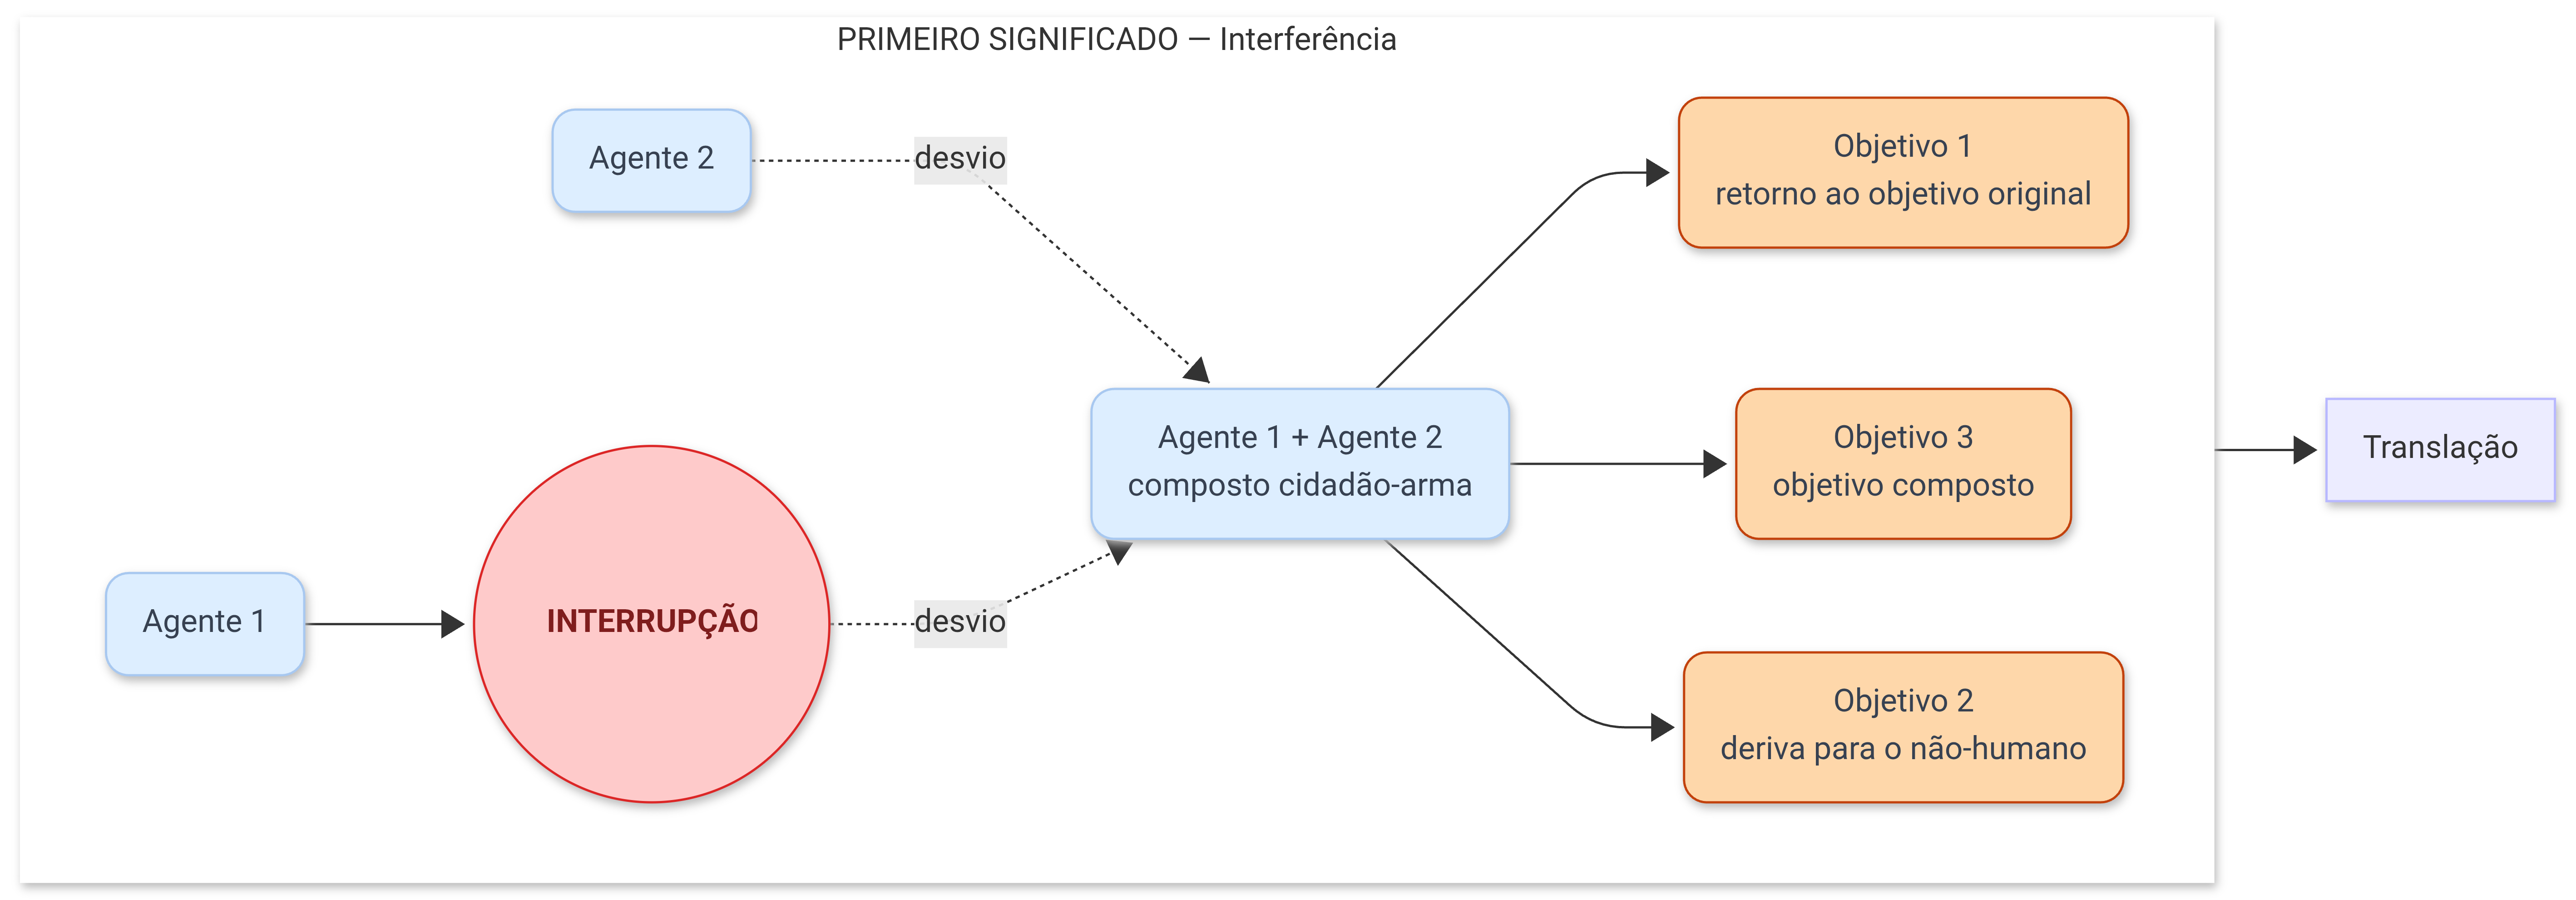
\includegraphics[width=0.6\linewidth]{figuras/cap.2/diagramas/mediacaosignificado_1_traducao.png}
    \caption[Primeiro significado da mediação técnica: tradução de objetivos]{Primeiro significado da mediação técnica, a tradução de objetivos, segundo \textcite{Latour2017Esperanca} (Figura~6.1 do original). O objetivo do Agente~1 é interrompido, o Agente~2 entra por um desvio, e da composição dos dois resulta um terceiro programa de ação, que pode retornar ao objetivo de partida (Objetivo~1), derivar para o objetivo do não humano (Objetivo~2) ou estabilizar-se em um objetivo composto (Objetivo~3). O eixo da translação ordena esses destinos.\url{https://mermaid.ai/d/f1c51456-43c3-424c-8edf-50566fbe40c2}}
    \label{fig:mediacao_significado_1}
\end{figure}

O segundo significado é a composição: a ação é propriedade de uma associação de atores, e não de um agente isolado. Leio aqui o exemplo do voo, que Latour resume na fórmula de que não é o piloto que voa, nem o avião, e sim a associação de aeroportos, pistas, planos de voo, sistemas de navegação, tripulação e companhia aérea. A competência e a ação são propriedades de toda a cadeia de actantes, e por isso a responsabilidade não se imputa a um só deles, e sim se distribui pela associação, no que Latour trata sob o princípio de simetria entre humanos e não humanos: ambos trocam propriedades ao longo das associações que os compõem. Cada agente cujo caminho é interrompido recruta um subprograma por desvio, e os subprogramas se aninham uns nos outros até comporem o objetivo comum, como mostra a Figura~\ref{fig:mediacao_significado_2}.

\begin{figure}[htbp]
    \centering
    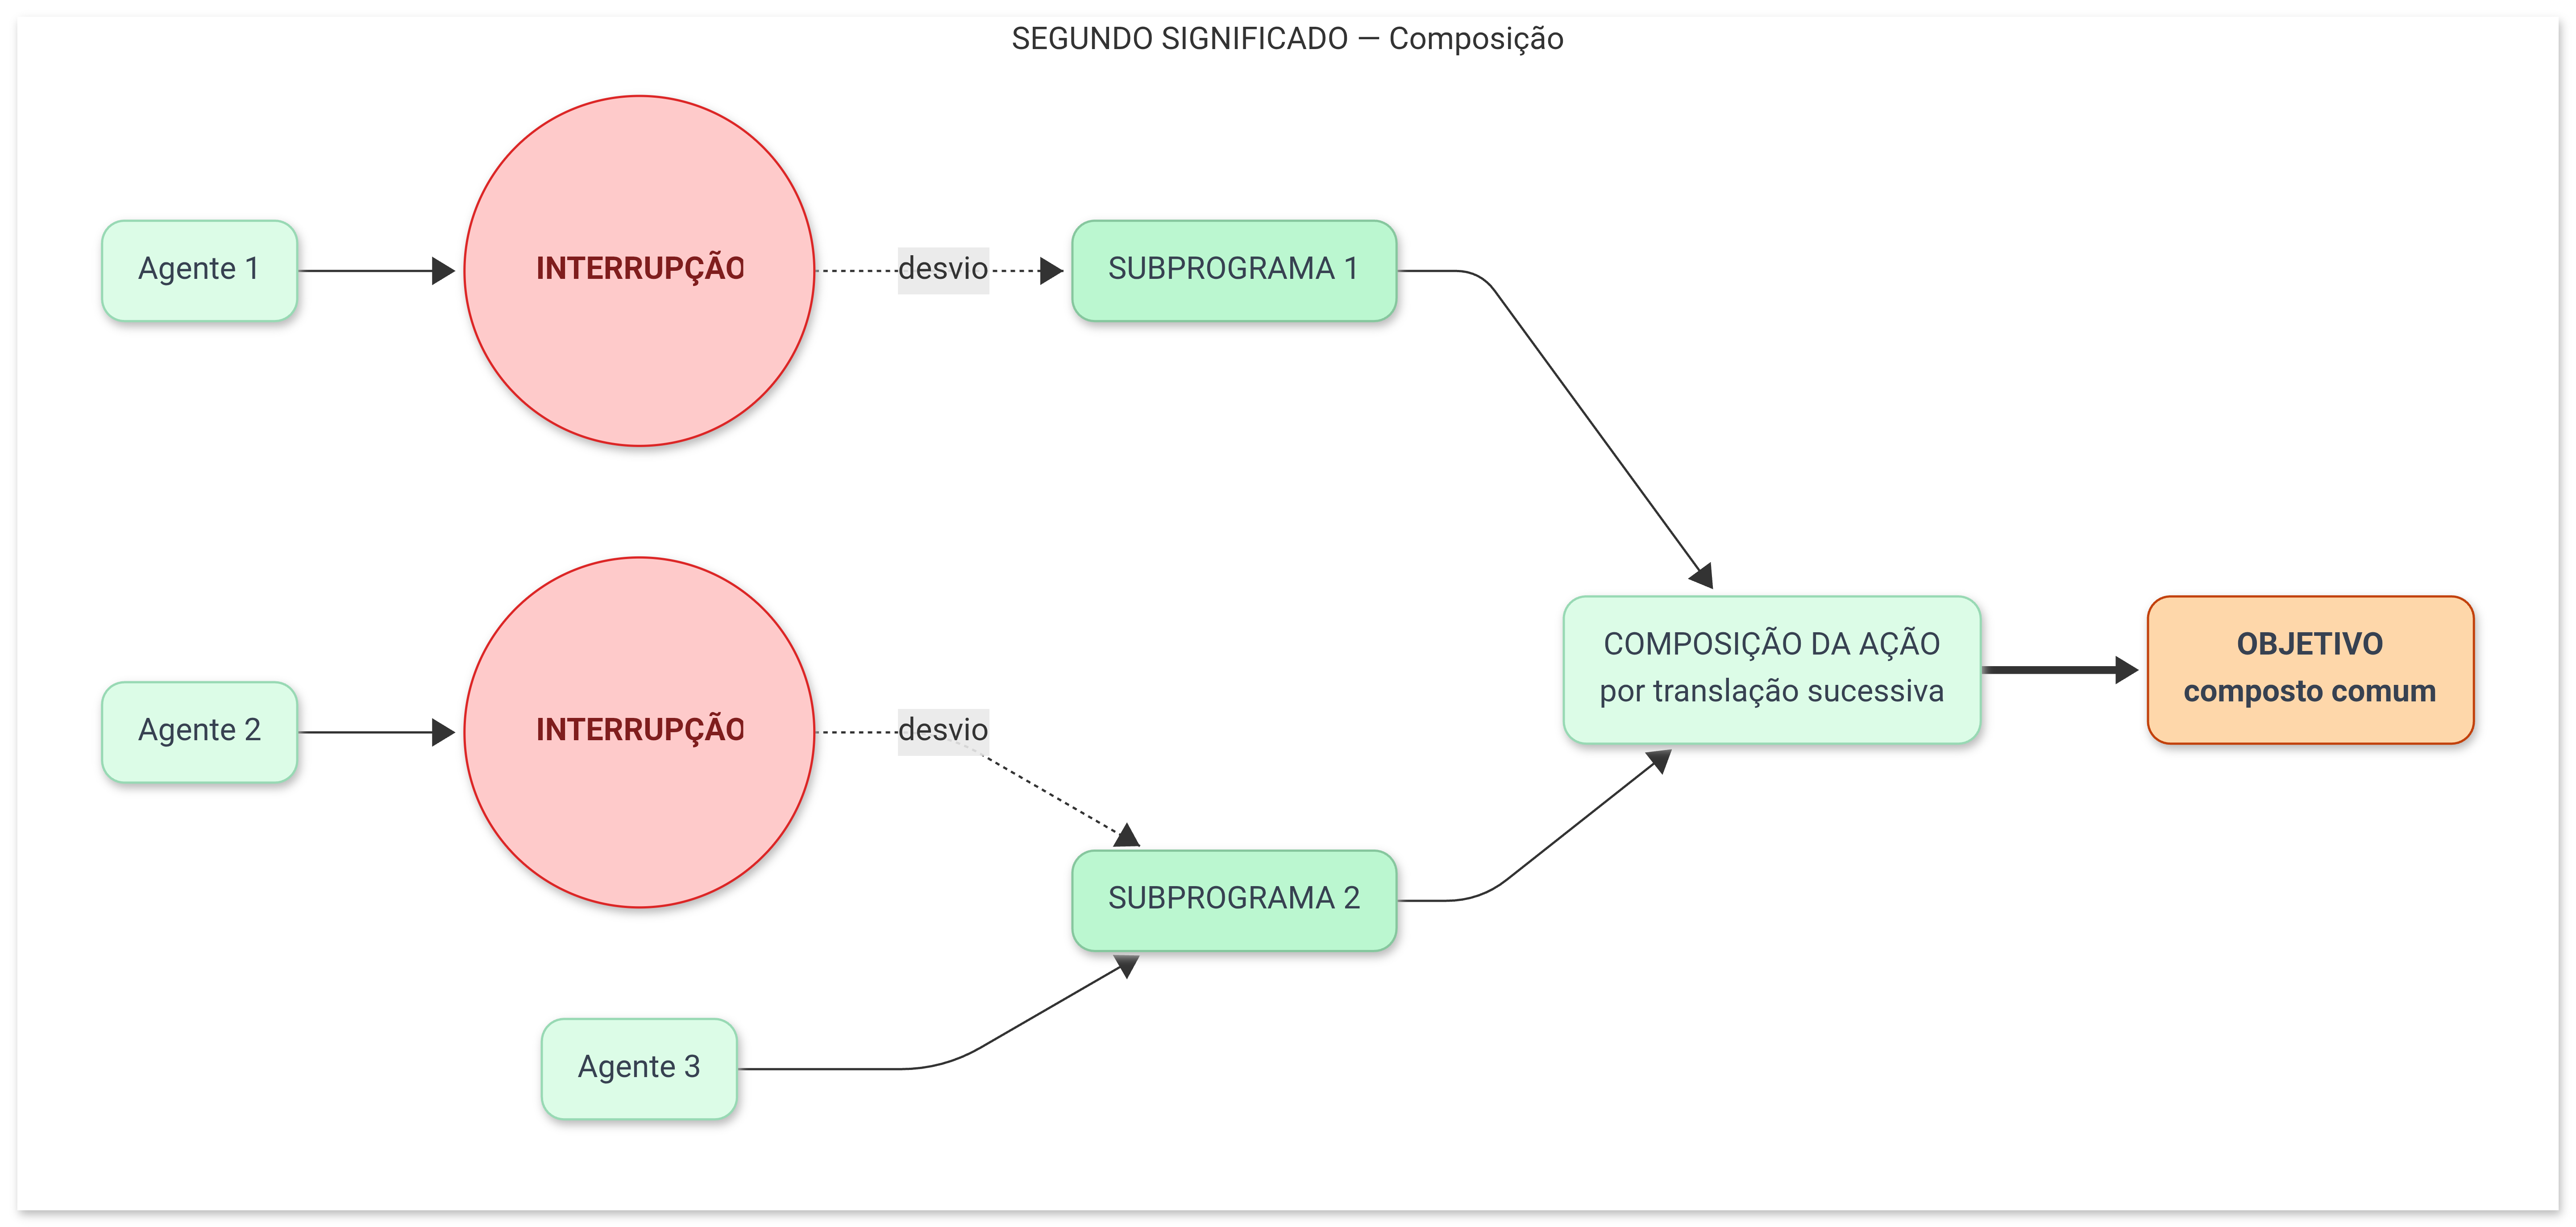
\includegraphics[width=0.6\linewidth]{figuras/cap.2/diagramas/mediacaosignificado_2_composicao.png}
    \caption[Segundo significado da mediação técnica: composição]{Segundo significado da mediação técnica, a composição, segundo \textcite{Latour2017Esperanca} (Figura~6.2 do original). Cada agente que tem o caminho interrompido recruta um subprograma por desvio, e os subprogramas se aninham uns nos outros. A ação é propriedade da associação inteira, e não de um agente isolado, de modo que o objetivo composto comum é alcançado pela composição da ação por translação sucessiva, representada pela linha que se alonga a cada passo acrescentado.\url{https://mermaid.ai/d/050e4650-4240-4681-b65d-825c33579f58}}
    \label{fig:mediacao_significado_2}
\end{figure}

O terceiro significado é o entrelaçamento de tempo e espaço, que Latour também nomeia obscurecimento reversível. Quando uma tecnologia funciona bem, fecha-se como caixa silenciosa, e o número de actantes que a compõem some de vista. Latour toma o retroprojetor que quebra no meio de uma palestra, e em torno do qual reaparecem subitamente as peças, as lâmpadas, os técnicos e os gestos antes invisíveis. O obscurecimento é reversível porque a unidade pode tornar a abrir-se e a fechar-se, e o objeto que contava por um passa a contar por muitos, ou por nenhum. É também aqui que se dá o entrelaçamento do tempo, porque o objeto carrega o trabalho congelado de pessoas distantes e ausentes que continuam a agir através dele no presente, e é por esse mecanismo que a sociedade ganha durabilidade e perdura pela incorporação desses mediadores não humanos, no argumento que Latour condensa no título de \enquote{Technology is Society Made Durable} \parencite{latour1991technology}. A Figura~\ref{fig:mediacao_significado_3} percorre os sete passos desse processo, do desintereste inicial à pontualização da unidade obscurecida.

\begin{figure}[htbp]
    \centering
    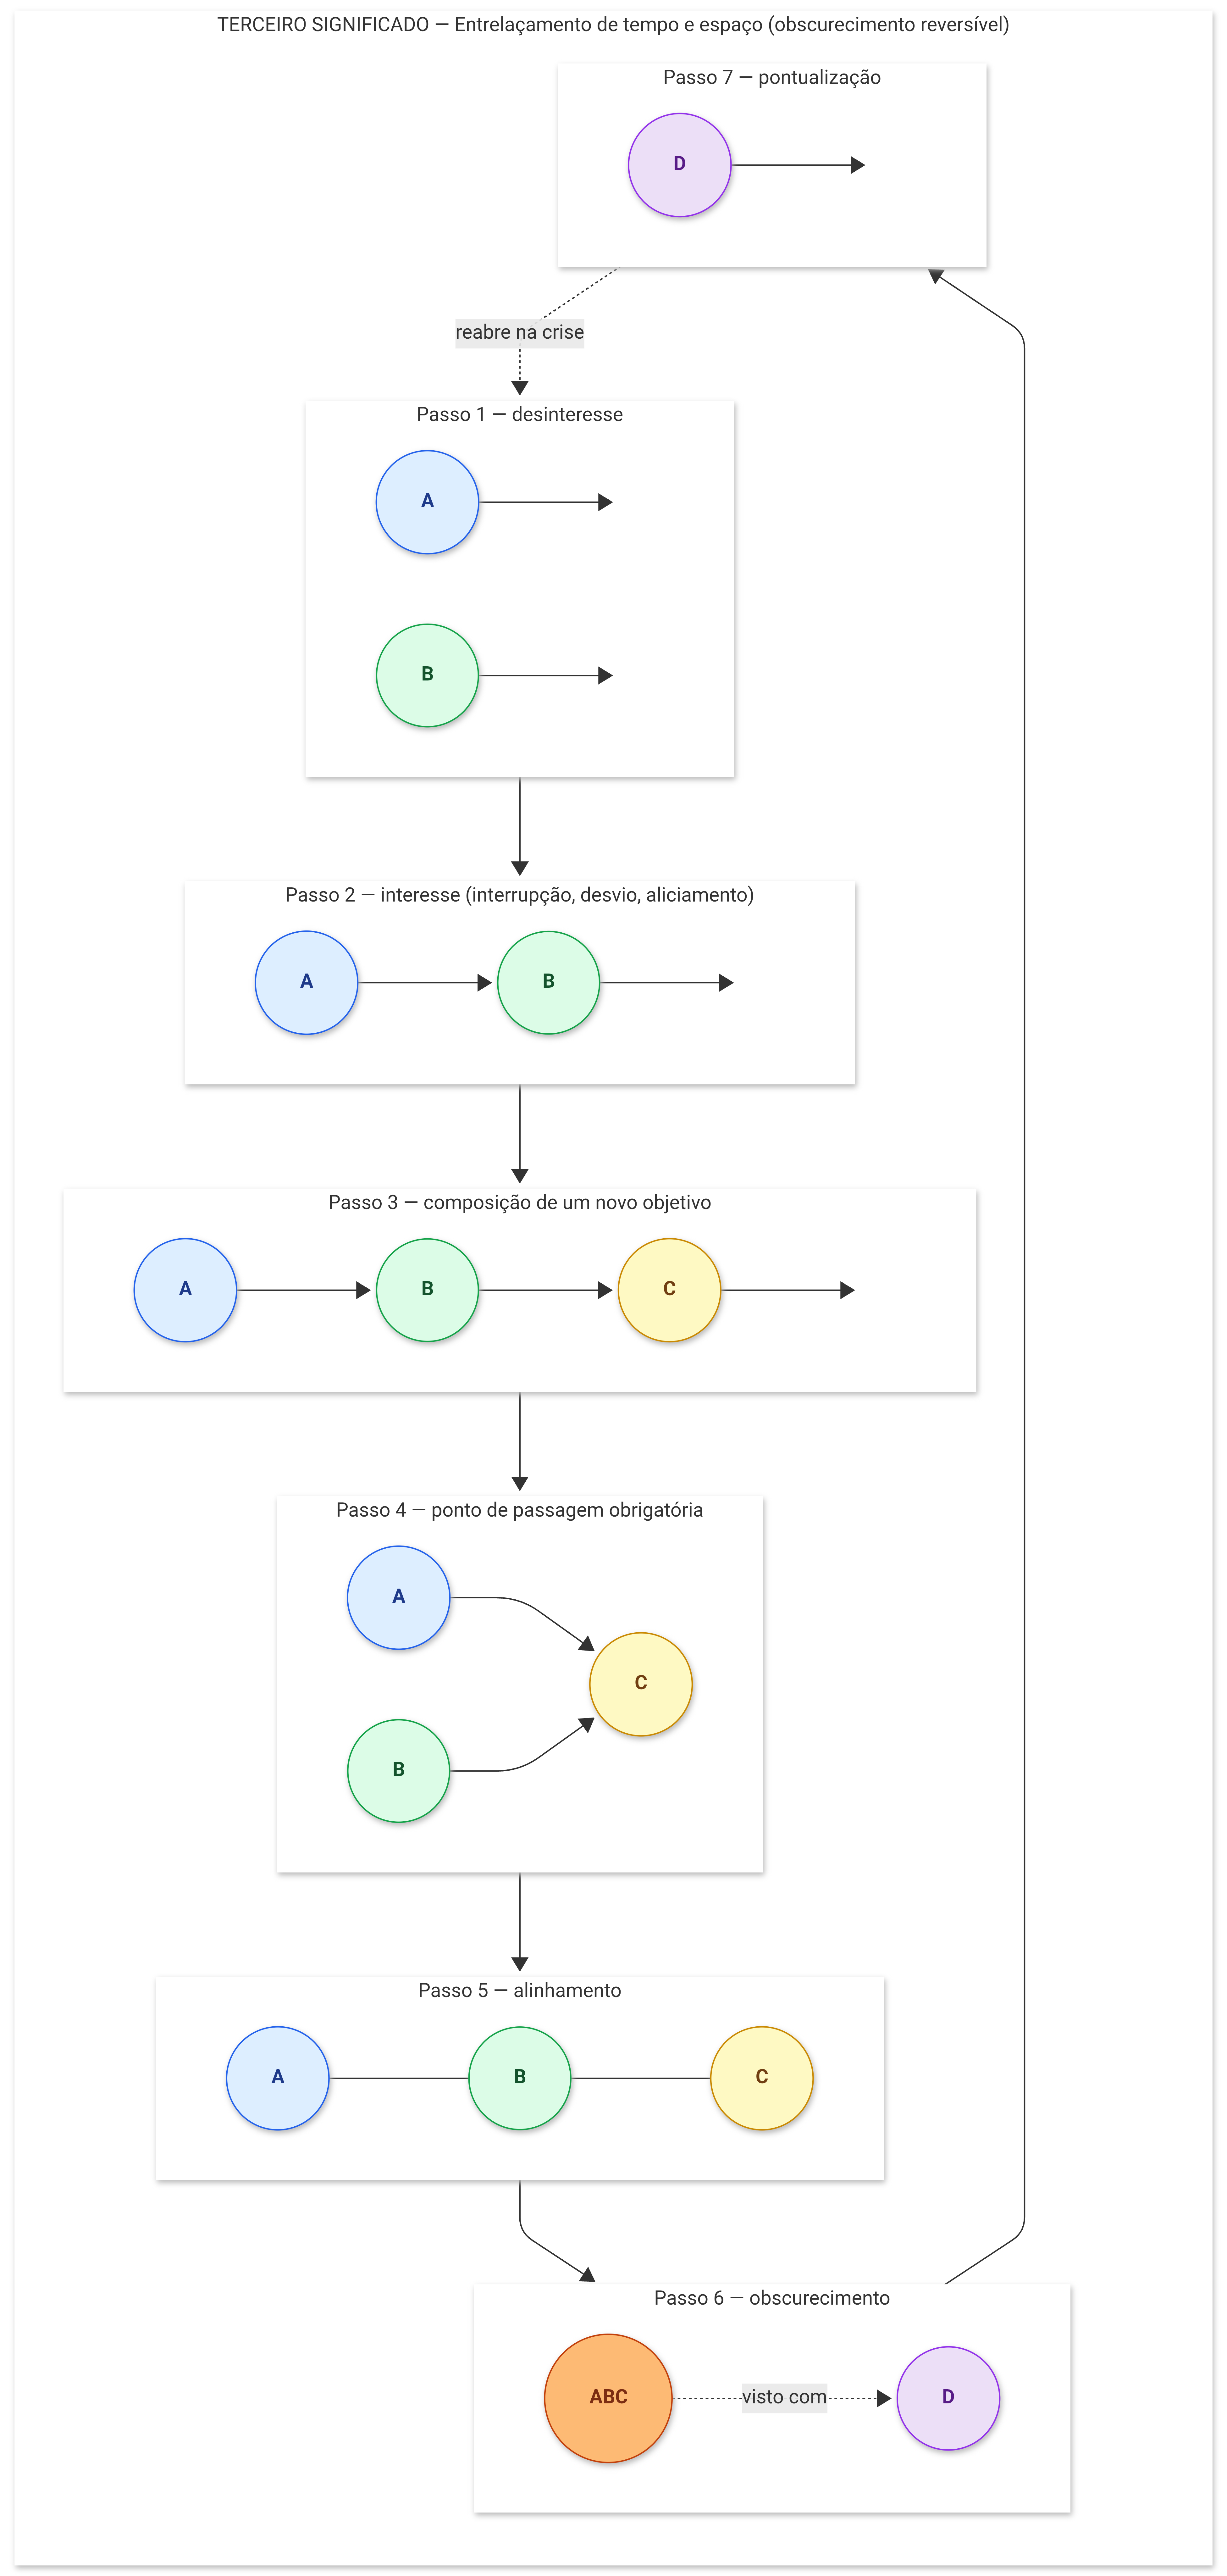
\includegraphics[width=0.5\linewidth]{figuras/cap.2/diagramas/mediacaosignificado_3_obscurecimento.png}
    \caption[Terceiro significado da mediação técnica: entrelaçamento de tempo e espaço]{Terceiro significado da mediação técnica, o entrelaçamento de tempo e espaço, que Latour descreve como obscurecimento reversível, segundo \textcite{Latour2017Esperanca} (Figura~6.3 do original). Os sete passos descrevem como agentes distintos (A, B e C, em cores próprias) deixam de seguir separados (desinteresse), passam a aliciar-se mutuamente (interesse), compõem um novo objetivo, convergem para um ponto de passagem obrigatória, alinham-se, e por fim se obscurecem em uma unidade que circula como um único actante (D, pontualização). As setas de dois sentidos marcam que o processo é reversível, porque a unidade obscurecida pode reabrir-se em uma crise e expor de novo os actantes que a compõem.\url{https://mermaid.ai/d/4b90c964-c828-4b60-ba05-d9b4ee409c69}}
    \label{fig:mediacao_significado_3}
\end{figure}

O quarto significado é a delegação, que Latour descreve como a transposição da fronteira entre signos e coisas: valores, deveres e ordens podem ser inscritos na matéria, de modo que objetos passam a prescrever comportamentos sem vigilância humana contínua. Latour toma o exemplo do quebra-molas (\emph{sleeping policeman}): em lugar de apelar à moralidade dos motoristas com uma placa de \enquote{devagar}, os engenheiros delegam essa ordem ao concreto, e o apelo ético se traduz em obstáculo físico sem deixar de permanecer prescrição, como mostra a Figura~\ref{fig:mediacao_significado_4}.

\begin{figure}[htbp]
    \centering
    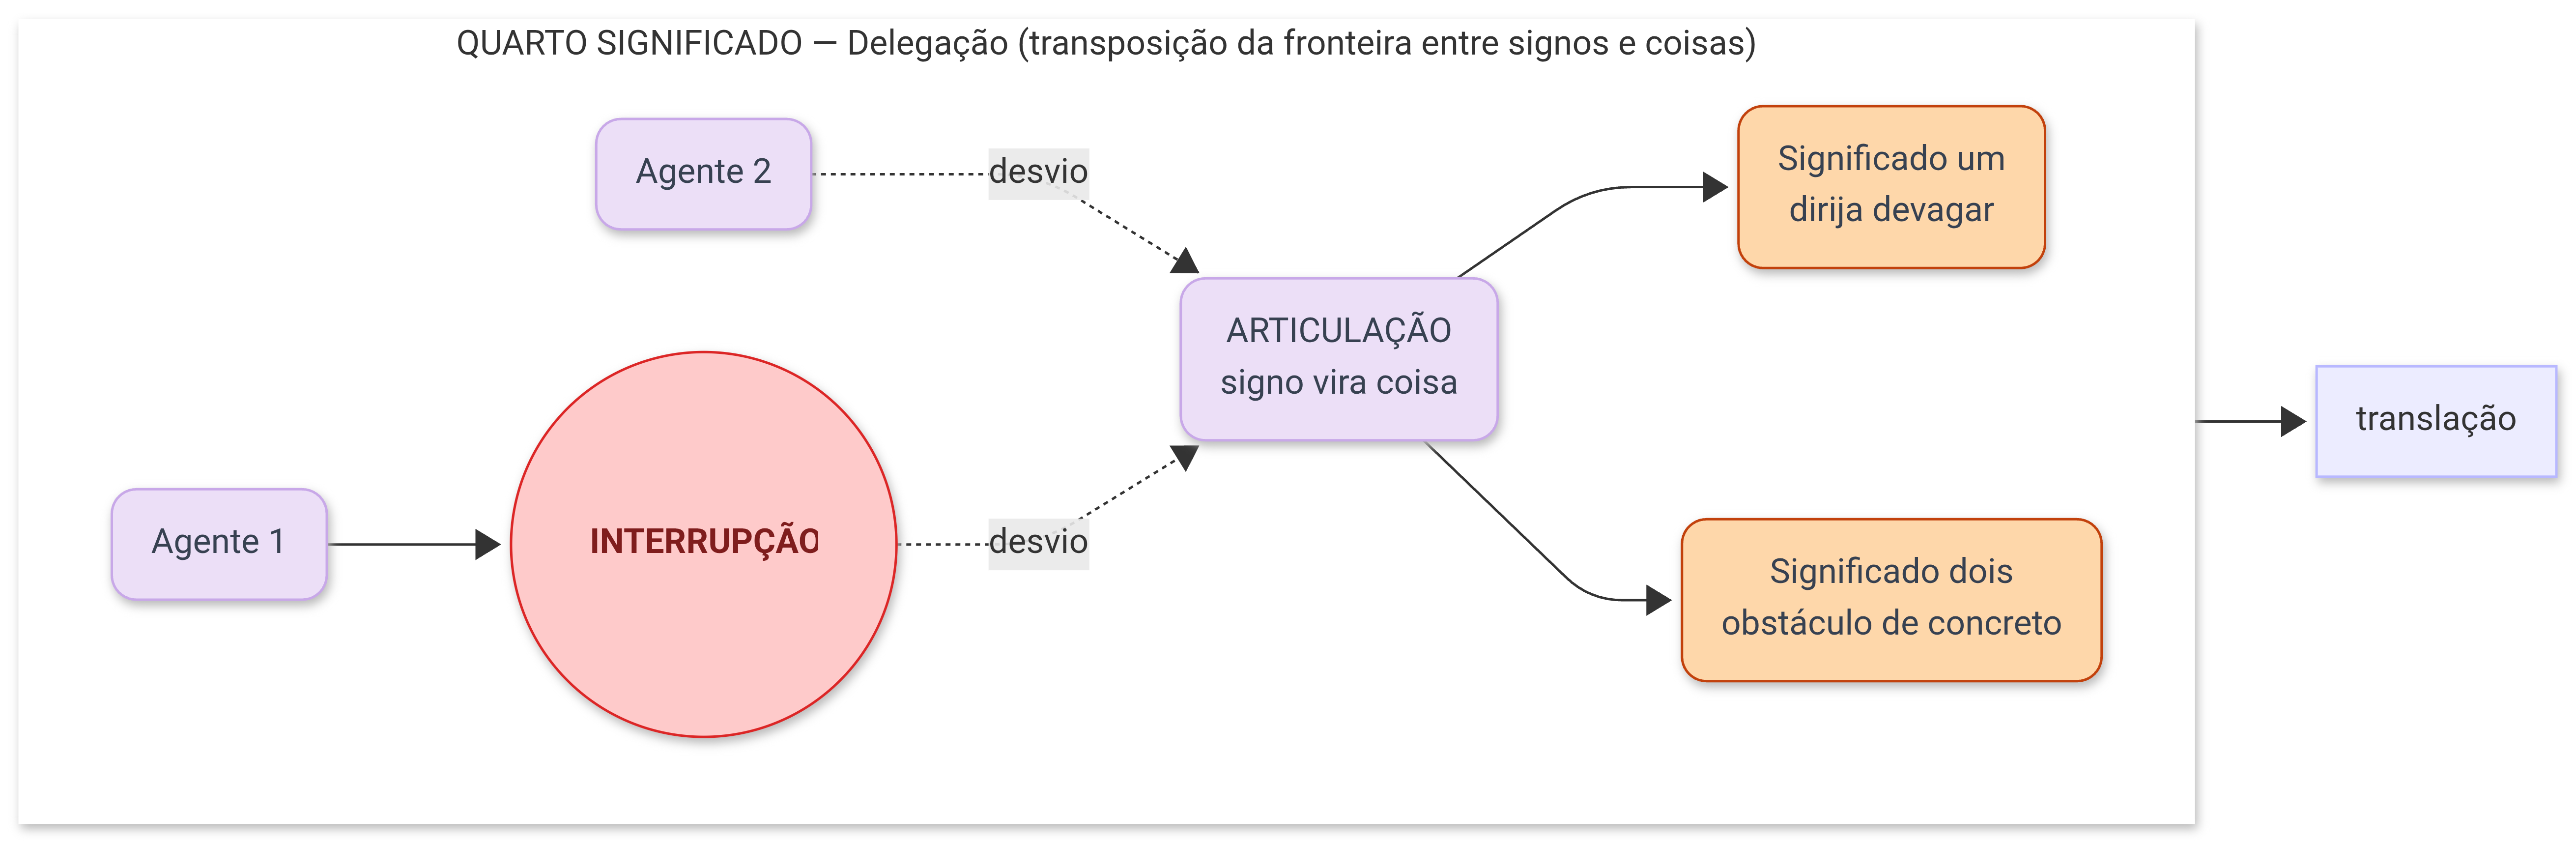
\includegraphics[width=0.6\linewidth]{figuras/cap.2/diagramas/mediacaosignificado_4_delegacao.png}
    \caption[Quarto significado da mediação técnica: delegação]{Quarto significado da mediação técnica, a delegação, que Latour descreve como transposição da fronteira entre signos e coisas, segundo \textcite{Latour2017Esperanca} (Figura~6.4 do original). A estrutura do desvio se repete, agora deslocando não o objetivo, e sim o próprio modo de expressão: um programa de ação humano, a norma \enquote{dirija devagar}, é inscrito na matéria, o quebra-molas, de modo que o Significado um (a prescrição) se traduz no Significado dois (o obstáculo de concreto), e o signo cruza a fronteira que o separa da coisa.\url{https://mermaid.ai/d/fb8411e2-65f0-4a16-a767-fad97bf15f8f}}
    \label{fig:mediacao_significado_4}
\end{figure}

% [NOTA DE REVISÃO 19] Parágrafo que ancora teoricamente a translação e a cadeia de translação, conceito que sustenta os capítulos 3 e 4 e que até aqui era redefinido do zero em cada um deles. Faz aqui, uma vez, a distinção Callon/Latour e a equivalência tradução/translação. As notas dos caps. 3 e 4 remetem a esta passagem. VERIFICAR chave Callon1986Sociology no .bib.
Detenho-me no primeiro significado, a tradução, porque é o que, ao se encadear com outros, sustenta a maior parte da descrição etnográfica que faço nos capítulos~\ref{capitulo3} e~\ref{capitulo4}. \enquote{Tradução} e \enquote{translação} vertem para o português a mesma palavra, \textit{translation} em inglês e \textit{traduction} em francês, e nomeiam o deslocamento pelo qual um actante, ao alistar outro, faz com que objetivos e interesses de partida distintos passem a coincidir, e produz com isso um vínculo que antes não existia e um terceiro programa de ação que nenhum dos actantes possuía sozinho \parencite{Latour2017Esperanca}. Michel Callon e Latour cunham o conceito nos textos fundadores da teoria ator-rede, e os dois o formulam em registros que mantenho distintos ao longo da tese. \textcite{Callon1986Sociology} descreve a translação como percurso de quatro momentos, a \textit{problematização}, o \textit{interessamento}, o \textit{recrutamento} e a \textit{mobilização}, pelos quais um actante se faz porta-voz de outros e desloca os interesses de cada um para um ponto de passagem comum; \textcite{Latour2017Esperanca} a formula como o primeiro dos quatro significados da mediação técnica, o deslocamento de objetivos na troca de propriedades entre humano e não humano. Os dois registros se completam, porque a translação de Callon descreve como os actantes se alistam, ao passo que a tradução de Latour descreve o que acontece com os objetivos de cada um quando o alistamento se dá. Chamo de cadeia de translação a sucessão desses deslocamentos quando um se encadeia ao outro, de modo que o objetivo traduzido por um actante se torna o ponto de partida traduzido pelo seguinte, e a inscrição produzida em uma etapa se torna a matéria-prima da etapa adiante. É essa figura, a do percurso em que cada elo transforma o que recebe do anterior antes de passá-lo ao próximo, que organiza a descrição da trajetória da \texttt{IBM} no capítulo~\ref{capitulo3}, do censo de Hollerith em 1890 à parceria com o \texttt{C4AI}, e a descrição do \texttt{Spira} no capítulo~\ref{capitulo4}, da voz do paciente no \enquote{covideiro} ao argumento científico que circula no artigo. Em ambos, o que sigo é a cadeia inteira de mediação, e por isso assento o conceito aqui, antes de entrar em campo.

% [NOTA DE REVISÃO 1] Parágrafo do radar: corrigida a duplicação "exemplo...exemplo", pontuação diversificada (regra 15).
A passagem do signo para a coisa abre complexidades adicionais quando passo a sistemas tecnológicos como a inteligência artificial. Latour toma o quebra-molas como caso, mas, se penso em um radar eletrônico de velocidade, que tem praticamente o mesmo objetivo, vejo que este alista uma rede muito maior: sensores, câmeras, bancos de dados de placas, sistemas de processamento, notificações automáticas e todo o aparato legal que converte a medição em multa. A mediação técnica deixa de apenas deslocar o apelo ético para o concreto, como no quebra-molas, e passa a multiplicar os actantes e as consequências, e torna a rede mais extensa e mais difícil de mapear à medida que cresce o número de mediações que sustentam uma única ação. Esse aumento de escala, que encadeia muitas traduções em uma só cadeia, é o que me leva dos objetos técnicos de Latour aos sistemas de inteligência artificial.

Os pesquisadores da IA vêm tocando nesse problema por outros caminhos. Durante um seminário transmitido pelo \texttt{C4AI}, no contexto da série \textit{Perspectives in AI}, Cláudio Pinhanez apresentou o problema através da constatação de que a IA generativa produz bons \emph{outputs} para a maioria dos usuários na maior parte do tempo \parencite{Pinhanez2026Seminar}. A fórmula funciona, em sua exposição, como ponto de partida de um deslocamento argumentativo, porque o que ela descreve é a sua intermitência, e não a sua confiabilidade. Em trabalho experimental, \textcite{Pinhanez2025Small} submeteram modelos pequenos, de dois a oito bilhões de parâmetros, a repetições da mesma pergunta, e verificaram que esses modelos com frequência respondem de modos diferentes a cada vez que a pergunta lhes é refeita, ainda que nada na pergunta tenha mudado. A inconsistência é mais aguda justamente nos modelos pequenos, que rodam em infraestrutura modesta e estão mais ao alcance de quem não dispõe de grande capacidade computacional, ao passo que os modelos médios, de cinquenta a oitenta bilhões de parâmetros, e os grandes, na casa dos trilhões, respondem de maneira bem mais estável.\footnote{Pinhanez expõe esses dados na palestra \enquote{The Non-Determinism of LLMs and Other Stability Issues of GenAI}, no seminário \textit{Perspectives in AI} do \texttt{C4AI}, em 29 de abril de 2026, disponível em \url{https://www.youtube.com/watch?v=wiewz65Tg6E} \parencite{Pinhanez2026Seminar}. Na exposição, ele situa o não determinismo como uma de duas instabilidades da IA generativa, ao lado da ausência de limitação local (\textit{local boundedness}), que torna difícil garantir a segurança desses sistemas.} O ponto decisivo é que essa inconsistência é propriedade do próprio mecanismo, e não defeito a corrigir, porque a geração de cada palavra resulta de um sorteio probabilístico, de modo que o mesmo sistema, diante da mesma entrada, pode devolver respostas diferentes a cada passagem. Pinhanez descreve esse traço como uma \enquote{falta de continuidade local, o que torna esses modelos imprevisíveis e incontroláveis}.\footnote{No original: \enquote{GenAI models suffer from lack of local continuity what makes them unpredictable and uncontrollable} \parencite[tradução minha]{Pinhanez2026Seminar}.}

% [NOTA DE REVISÃO 1] Inserida nota que distingue a IA generativa do algoritmo determinístico no sentido corrente, ancorada na primeira menção ao determinismo como princípio da ciência da computação. Trata a confusão comum entre os dois objetos.
Tomo esse fio de \textcite{Pinhanez2026Seminar, Pinhanez2025Small} e o cruzo com o conceito de mediação técnica de \textcite{Latour2017Esperanca} para descrever o que a IA generativa traz de novo. O determinismo era princípio inabalável para a ciência da computação até a IA generativa mostrar que é possível inserir indeterminação e descontinuidade em um sistema computacional, e é esse traço que devolve a discussão à mediação técnica e, ao mesmo tempo, expõe onde ela encontra um objeto que os artefatos de Latour não anteciparam.\footnote{Vale distinguir a IA generativa do algoritmo no sentido corrente, porque os dois são com frequência tomados um pelo outro. Um algoritmo, na acepção clássica da ciência da computação, é uma sequência finita de instruções explícitas que, dada a mesma entrada, produz sempre a mesma saída, e cujo percurso pode ser lido e auditado passo a passo, da ordenação de uma lista ao cálculo de uma rota. É determinístico e inspecionável por construção. A IA generativa não funciona assim. Embora seja executada sobre algoritmos, ela não consiste em regras escritas por um programador, e sim em bilhões de parâmetros ajustados sobre dados de treinamento, dos quais a saída emerge por um sorteio probabilístico a cada termo gerado. Daí as duas propriedades da IA generativa que descrevo nesta seção, o não determinismo e a opacidade, que o algoritmo clássico justamente não tem.}

Sintetizo na figura~\ref{fig:diferencial_ia_mediacao} o que a IA generativa acrescenta à mediação técnica de Latour, e o faço por contraste. O mediador técnico que Latour descreve transforma o que transmite, e nisso a IA generativa não difere de nenhuma outra técnica. A diferença está em outro lugar, e tem três faces que o diagrama dispõe lado a lado. A primeira é que a IA generativa é uma cadeia imensa de mediadores, e não um mediador único: de um lado, os insumos que compõem cada modelo, os dados de treinamento, o trabalho de anotação, o corpus e a curadoria, os parâmetros aprendidos e a infraestrutura de processamento; de outro, os vários modelos de IA que se encadeiam em um sistema em uso, dos quais o modelo generativo é apenas um, ao lado de reconhecedores de fala e visão, modelos de busca e \emph{embedding}\footnote{Um \emph{embedding} é a representação de uma palavra, imagem ou outro dado como um vetor de números, isto é, como um ponto em um espaço de muitas dimensões em que a proximidade entre pontos corresponde a alguma semelhança de sentido ou de uso. O termo vem do aprendizado de máquina, onde nomeia tanto esse modo de representar os dados quanto o modelo que os converte em vetores, e é com base nessa proximidade vetorial que sistemas de busca recuperam itens parecidos com uma consulta. Mantenho o termo em inglês, em vez de traduzi-lo por \enquote{vetor de incorporação} ou \enquote{imersão}, porque é nessa forma que circula entre os pesquisadores com quem convivi em campo.} e classificadores de moderação. A composição que Latour descreve no segundo significado da mediação se multiplica aqui, e cada elo acrescenta a sua própria transformação ao que atravessa a cadeia. A segunda face é o não determinismo. No caso mais controlado que se pode medir, a mesma pergunta feita pelo mesmo usuário e repetida de modo idêntico, a resposta já muda a cada repetição, porque a geração de cada termo resulta de um sorteio probabilístico, e os estudos de \textcite{Pinhanez2025Small} encontram, nos modelos pequenos, consistência em apenas metade a quatro quintos dos casos. Se mesmo nesse caso mínimo a saída varia, a variação só aumenta quando as condições se abrem para usuários, perguntas e formulações distintas, ainda que esse cenário aberto exceda o que o experimento mediu. A terceira face é a não explicabilidade, e o diagrama a formula com cuidado para não sugerir que os engenheiros ignorem o que fazem. Eles conhecem a arquitetura do modelo, os dados com que o treinaram e cada operação que ele executa, e medem o seu comportamento no agregado. O que não conseguem é rastrear, em termos causais legíveis, por que aquela resposta particular saiu daquela vez, porque ao reabrir a caixa não há uma regra escrita a inspecionar, e sim bilhões de parâmetros cuja interação produz a saída sem passar por nenhuma formulação legível. É nesse ponto que a caixa-preta da IA se separa da de Latour. O obscurecimento que descrevi no terceiro significado é reversível justamente porque o que a caixa esconde são mediadores identificáveis um a um, regras e peças que se pode reabrir e conferir, ao passo que a opacidade do modelo persiste mesmo com a caixa aberta. A IA generativa é, então, um mediador no sentido pleno de Latour, e é também um mediador composto por uma multidão de outros mediadores, não determinístico na saída e opaco na decisão, ainda quando tudo o que o constitui é conhecido.

\begin{figure}[htbp]
    \centering
    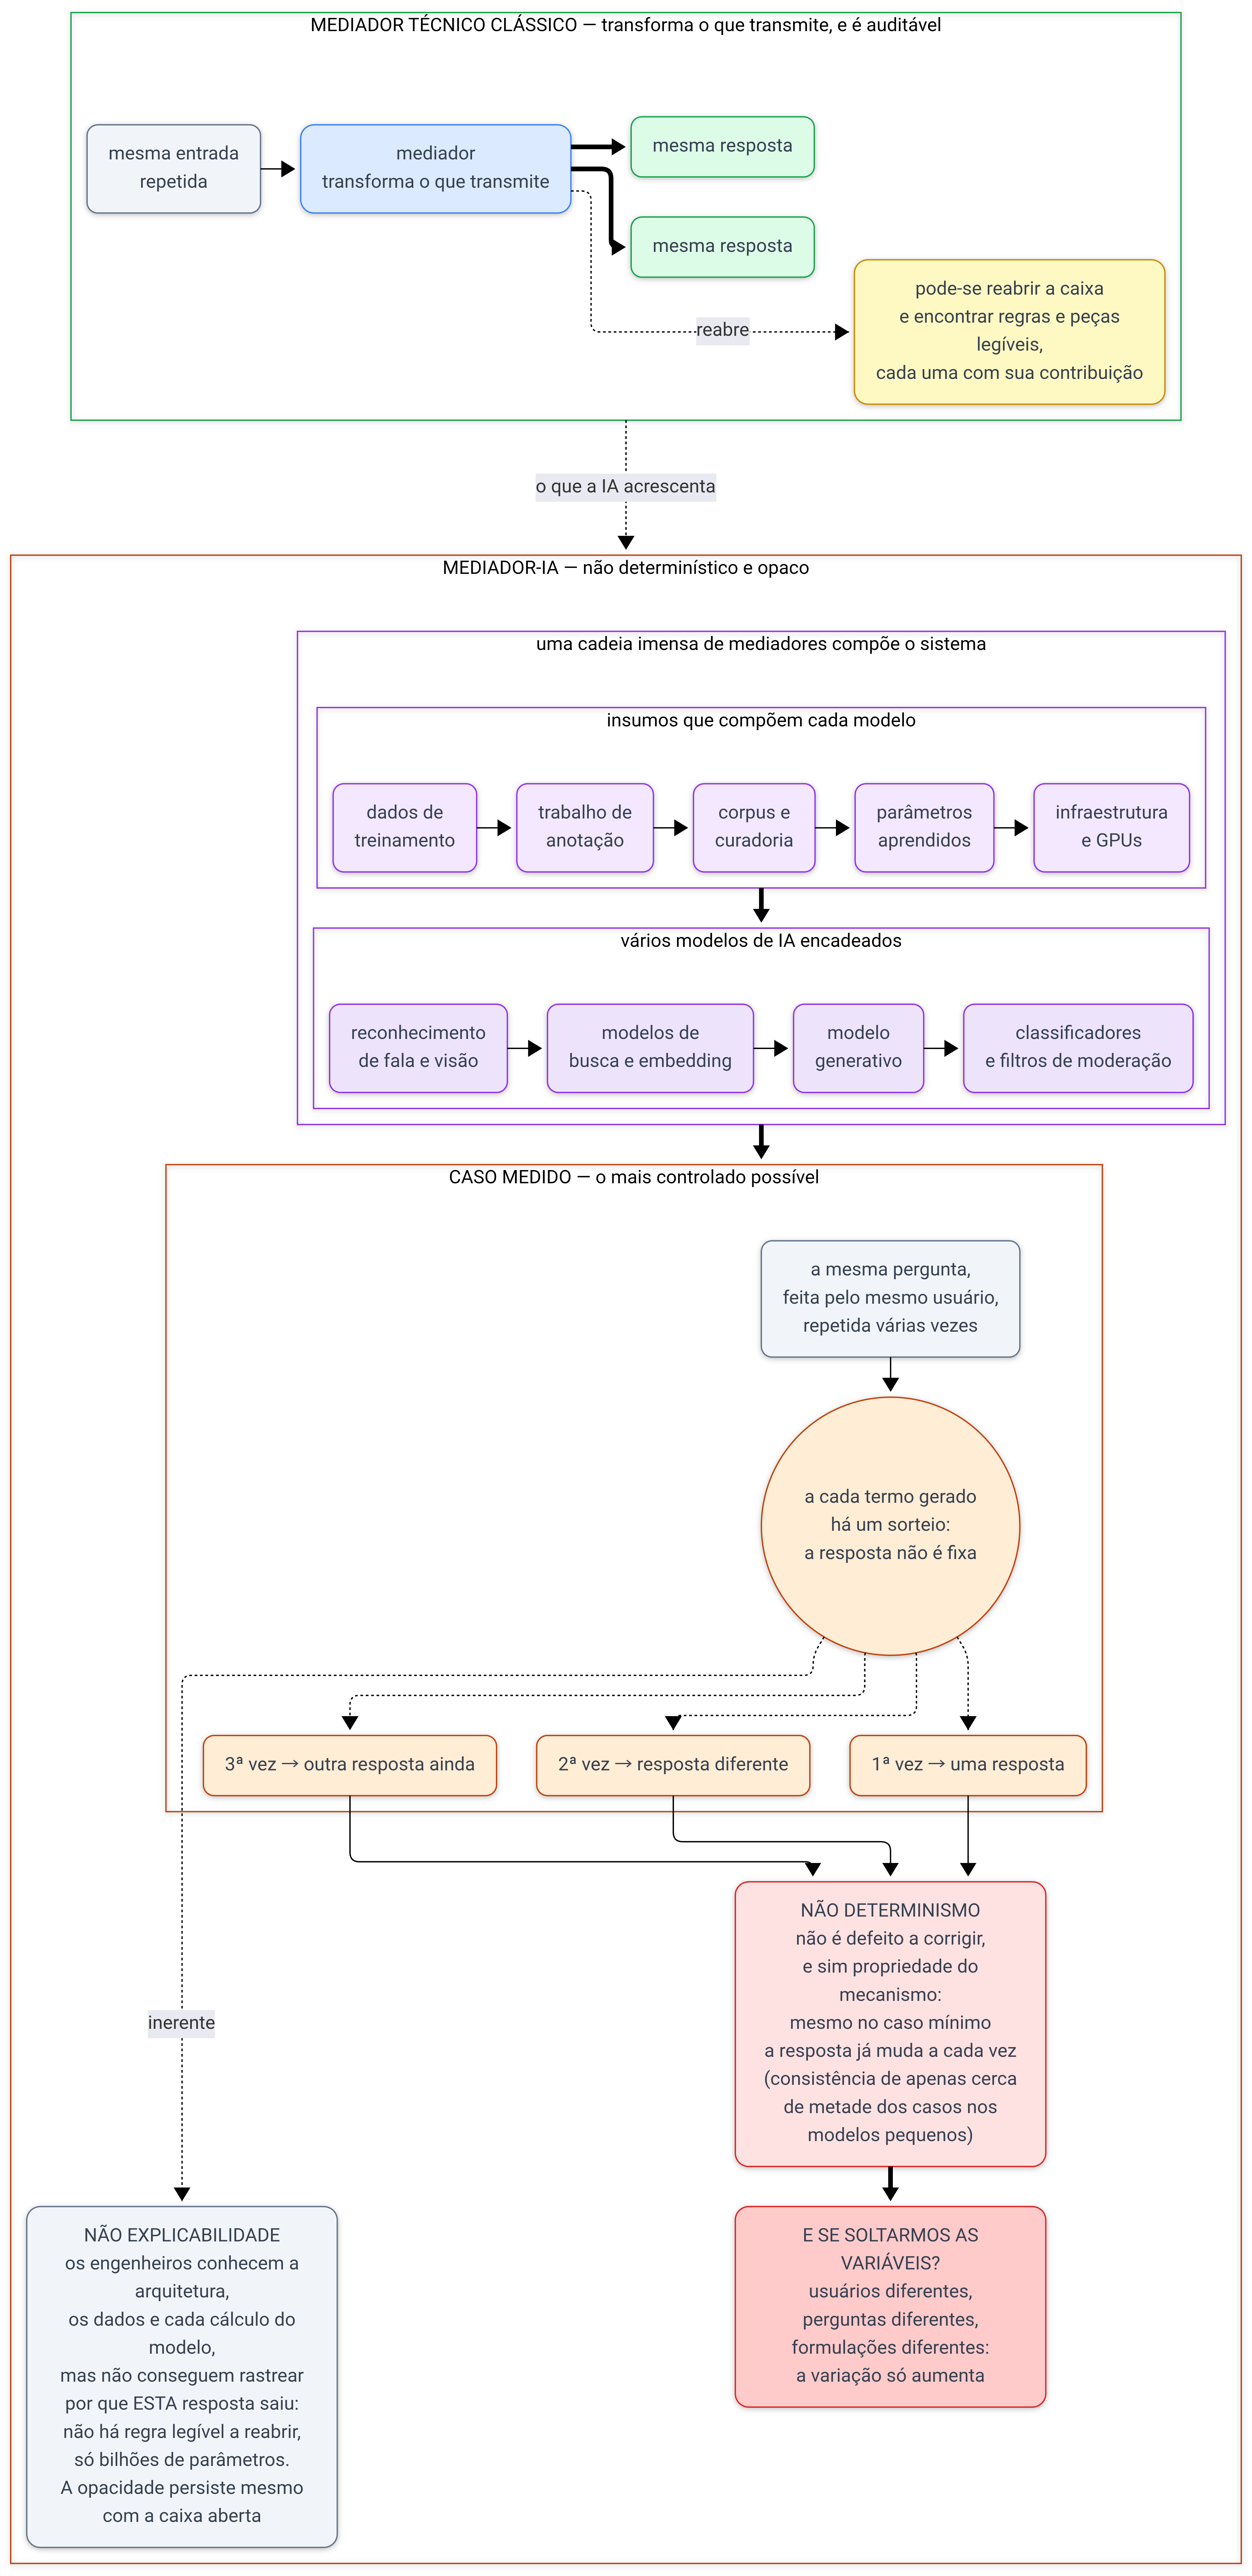
\includegraphics[width=0.5\linewidth]{figuras/cap.2/diagramas/cadeia-mediacao-ia-capitulo2.png}
    \caption[O diferencial da IA generativa na mediação técnica]{O diferencial da IA generativa diante da mediação técnica de Latour. À esquerda, o mediador técnico tal como Latour o descreve: transforma o que transmite, devolve a mesma saída à mesma entrada repetida, e pode ser reaberto e auditado, porque o que a caixa esconde são regras e peças legíveis, cada uma com sua contribuição. À direita, o mediador-IA: o sistema é composto por uma cadeia de mediadores, dos insumos de cada modelo, dados, anotação, corpus, parâmetros e infraestrutura, aos vários modelos de IA encadeados, dos quais o generativo é apenas um. No caso mais controlado que se pode medir, a mesma pergunta feita pelo mesmo usuário e repetida várias vezes, a resposta já muda a cada repetição, porque a geração de cada termo passa por um sorteio probabilístico, e a variação só aumenta quando as condições se abrem para usuários, perguntas e formulações distintas. A caixa permanece opaca mesmo aberta, dado que os engenheiros conhecem a arquitetura, os dados e cada operação do modelo, mas não conseguem rastrear por que aquela resposta particular saiu, já que não há regra legível a reabrir, e sim bilhões de parâmetros.\url{https://mermaid.ai/d/9b29f69e-2c76-465a-b25f-033401bf57c5}}
    \label{fig:diferencial_ia_mediacao}
\end{figure}


A falta de explicabilidade modifica a forma como concebemos a confiabilidade, pois o funcionamento interno do sistema permanece opaco mesmo quando “se abre a caixa” e o que se acessa são apenas inúmeros parâmetros, sem que essa quantidade se converta na regra que efetivamente produziu uma determinada resposta. É isso que permanece não explicável para os desenvolvedores. Tornar o sistema explicável em termos causais vai além do que as arquiteturas atuais permitem; porém, registrar e divulgar o que as medições mostram sobre o comportamento do sistema está, sim, ao alcance de quem o projeta, em que domínios ele tende a alucinar, em que tipos de pergunta a inconsistência é mais frequente, em que cenários a falta de continuidade local se torna mais acentuada. Os dados apresentados por \textcite{Pinhanez2025Small} sobre taxas de inconsistência em função do tamanho do modelo são justamente esse tipo de transparência. Já aos usuários cabe outra tarefa, utilizar os sistemas levando em conta as limitações que os desenvolvedores precisam identificar e explicar. São duas responsabilidades diferentes, e misturá-las produz efeitos importantes, porque, quando a transparência falta do lado de quem constrói, o trabalho de mapear as limitações recai sobre quem usa, não por meio do letramento crítico, mas por tentativa e erro, às custas do usuário e em favor de quem reteve a informação.\footnote{Aproximo essa distinção no capítulo~\ref{capitulo1}, na subseção~\ref{subsec:compostagem3}, em que argumento que a narrativa de \emph{AI literacy} funciona de forma ambígua, ao mesmo tempo em que expressa uma demanda legítima de quem pretende usar IA com autonomia crítica, ela também funciona como deslocamento que transfere ao usuário o encargo de suprir falhas que os desenvolvedores não comunicaram.} Distinguir o que cabe a cada parte é condição para atribuir responsabilidade a quem de fato a detém, em vez de movê-la por completo para o lado do usuário.

O argumento da responsabilidade distribuída tem consequências que excedem o plano da composição individual entre o sistema e o usuário, e que por meio do conceito de mediação técnica é possível aprofundar. Se os desenvolvedores não cumprem a responsabilidade de documentar e comunicar as limitações que conseguem medir, uma das respostas possíveis é a regulação que impeça a circulação de sistemas que não consigam demonstrar a confiabilidade que anunciam.\footnote{O \emph{AI Act} europeu (Regulamento 2024/1689), em vigor desde agosto de 2024, classifica sistemas de IA por nível de risco e impõe requisitos de transparência, documentação e auditoria que variam conforme a classificação. Sistemas de alto risco, incluídos os usados em saúde, educação e emprego, estão sujeitos a avaliação de conformidade antes de chegar ao mercado.} O enquadramento que responsabiliza as empresas que desenvolvem os sistemas é necessário, mas também é insuficiente, porque os erros dessas tecnologias, as alucinações, os vieses de treinamento, a inconsistência que \textcite{Pinhanez2025Small} medem, têm sido tratados como falhas técnicas que melhorias futuras irão corrigir; essa abordagem obscurece que são também parte de um projeto econômico-político que decide o futuro da IA por uma visão de mundo específica: mais dados, mais parâmetros e maior velocidade de lançamento são sempre preferíveis, e os custos dos erros são externalidades que os usuários e a sociedade acabam por absorver \parencite{Brennan2025ArtificialPower}. Essa visão de mundo é produzida e sustentada por uma rede de atores/actantes que inclui empresas de modelos de linguagem, fabricantes de chips e infraestrutura computacional, fundos de investimento que financiam o ritmo de lançamento, pesquisadores que transitam entre academia e indústria, instituições que legitimam os resultados e reguladores que podem favorecer ou beneficiar esse projeto tecnológico. Os debates sobre ética e responsabilidade na IA ganham em precisão quando tomam essa rede como interlocutor, em lugar de cada sistema ou empresa isoladamente. É nesse ponto que a fotografia que abre esta tese, a figura~\ref{fig:dgx1-openai}, com Jensen Huang entregando o DGX-1 a Elon Musk em 2016 enquanto a parede ao fundo anuncia que o destino do mundo depende do uso que se faz do conhecimento, retorna aqui para relacionar o momento em que a infraestrutura que tornaria possível treinar os sistemas que esta seção descreve foi entregue simbolicamente à organização que lançaria o \texttt{ChatGPT} sete anos depois, e o \texttt{C4AI}, herdeiro das possibilidades e dos problemas que essa rede traz consigo, como descrevi no capítulo~\ref{capitulo1}, é um de seus nós brasileiros. Depois de ter percorrido o que a mediação técnica da IA generativa faz e o que ela oculta, fica mais claro por que a tese se inicia com essa imagem e inscreve o problema que os capítulos seguintes perseguem em campo.

A mediação técnica que apresentei há pouco nos seus quatro movimentos aparece na fala de Cláudio de outra forma. Quando ele toma de empréstimo o lema do movimento pelos direitos das pessoas com deficiência, o \textit{nothing about us without us} \parencite{Pinhanez2026Seminar}, e sustenta que a confiabilidade é propriedade de um uso que distribui responsabilidade entre quem constrói, quem regula e quem usa, e não atributo do modelo tomado isoladamente, descreve o que Latour chama de composição, a ação como propriedade de uma associação de actantes. A mediação técnica que trago de Latour e a confiabilidade distribuída que Cláudio mede conectam-se de modo \textit{merográfico}, no sentido que \textcite{strathern2000pse} dá ao termo: formam um par, e cada conceito permanece preso ao seu próprio universo de sentidos, de modo que o que define um não é o que define o outro \parencite[p.~248]{strathern2000pse}.\footnote{O conceito merográfico (do grego \textit{méros}, parte, e \textit{-gráphein}, descrever), que Strathern desenvolve em \textit{Property, Substance and Effect} \parencite{strathern2000pse}, designa uma forma de conexão em que algo se liga a outra coisa por um de seus aspectos, sem que a junção produza uma relação recíproca ou mutuamente definidora. No original, ao analisar o par de Radin entre valores de mercadoria e de não-mercadoria: \enquote{this joining does not yield a reciprocal or mutually defining relation} \parencite[p.~248]{strathern2000pse}. Cada termo do par, escreve Strathern, recorre ao seu próprio universo de conotações, aplicações e sentidos, e é nessa coexistência sem fusão, e não em alguma síntese, que reside o efeito etnográfico da comparação.} Os dois descrevem a agência e a responsabilidade como distribuídas ao longo de uma cadeia de associações entre humanos e não humanos, porém, com efeitos distintos resultantes dessas cadeias. A indeterminação que a análise de \textcite{Pinhanez2025Small} mede, a falta de continuidade local que torna os modelos de IA generativa imprevisíveis, é um problema a resolver, e a confiabilidade distribuída, uma propriedade a garantir. Para a teoria ator-rede, essa mesma indeterminação é constitutiva da translação, que desloca o objetivo a cada translação, dessa maneira, a distribuição da agência não é atributo a aferir, é mais uma cadeia a seguir. É nessa conexão merográfica, em que o mesmo conceito comparece de um lado para nomear um problema a resolver e de outro para descrever uma cadeia a seguir, que está o interesse do cruzamento desses fios.

O cruzamento também faz com que a mediação técnica deixe de ser um conceito que aplico de fora e passa a ser o fio com que sigo, em campo, uma cadeia concreta de translações a partir dos conceitos dos próprios actantes/atores: seja na trajetória da \texttt{IBM} que o capítulo~\ref{capitulo3} segue do censo de Hollerith ao \texttt{C4AI}, e o \texttt{Spira} que o capítulo~\ref{capitulo4} segue desde a voz do paciente às fórmulas e aos gráficos que circulam no artigo científico. O capítulo~\ref{capitulo4} mostra ainda como o conceito de \emph{pipeline}, corrente na ciência da computação, também dialoga com a mediação técnica.\footnote{Um \emph{pipeline}, na ciência da computação, divide um processo em uma série de etapas sequenciais e conectadas, em que a saída de cada etapa é a entrada da seguinte, e é assim que a área identifica e rastreia as associações que faz. A descrição se aproxima da translação latouriana, a cadeia em que cada elo recebe o que o anterior lhe passa e entrega ao próximo, mas os dois conceitos se conectam de modo merográfico: para Latour, a translação desloca o objetivo a cada passagem, e desse deslocamento emerge um terceiro programa de ação que nenhum elo possuía isoladamente, de modo que a transformação é a condição do encadeamento; o \emph{pipeline}, ao contrário, é desenhado para que a saída de uma etapa seja exatamente a entrada que a próxima espera, sem resto e sem desvio, e nele a transformação não prevista conta como erro a corrigir. O capítulo~\ref{capitulo4} acompanha o que acontece quando a translação que a engenharia tenta conter em \emph{pipeline} previsível reintroduz, no \texttt{Spira}, os deslocamentos que o desenho buscava suprimir.} Trazer os conceitos da tecnociência na forma em que os próprios atores os usam mostra que o entendimento dos fenômenos e dos efeitos que esses conceitos nomeiam se faz no cruzamento entre os fios --- os meus e o deles, emaranhados de onde sempre se fazem \enquote{nós}. 

Até aqui acompanhei a mediação da IA generativa observando o que o sistema faz com aquilo que o atravessa e com o que ele oculta: a cadeia de mediadores, o caráter não determinista da saída e a opacidade de como chegou aos resultados que entrega. Agora sigo a mesma cadeia em direção ao que compõe o sistema, porque o conhecimento, os saberes e os dados que o formam não estão fora da mediação. São também mediação que se prolonga para o interior do sistema: cada dado de treino, cada anotação, cada decisão de curadoria é, por si só, uma translação, uma troca de propriedades em que o conhecimento de uma multidão é deslocado, recortado e inscrito no modelo.

A primeira dessas trocas que compõem o sistema é a que nele torna presente o conhecimento coletivo acumulado.\footnote{Matteo Pasquinelli sintetiza a IA como captura da \enquote{inteligência coletiva} que se ergue sobre vastos repositórios de herança cultural e de trabalho coletivo \parencite {Pasquinelli_EyeMaster_2023}. Abordo essa questão com mais detalhes na seção \ref{sec:predicao_poder}.} Esse conhecimento coletivo entra no sistema de IA de forma concreta. Os grandes modelos de linguagem, que funcionam por meio do processamento de linguagem natural e aprendizado de máquina, geram linguagem humana com uma fluência até então inédita, e o fazem porque foram treinados sobre vastos conjuntos de dados que reúnem, em sua maior parte, a produção de inúmeros autores, culturas e contextos, recolhida da internet sob condições de autorização variadas e quase sempre de forma não transparente e por vezes indevida. O que entra no modelo são, assim, camadas de conhecimento, de valor e de expressão tão extensas quanto difíceis de rastrear até as suas origens. Antes, porém, de alimentar o treinamento, esses dados passam por um trabalho que costuma ficar fora de cena, pois alguém precisa organizá-los, classificá-los e rotulá-los, decidir a que tema pertence um texto, se ele é ofensivo, se a resposta a uma pergunta é adequada, ou, quando o dado é uma imagem ou um áudio, o que ali está representado. É sobre os rotuladores que recai essa decisão, e é nas suas mãos que o conhecimento coletivo sofre o primeiro recorte antes de se inscrever no sistema.\footnote{Esse trabalho humano que sustenta sistemas anunciados como automáticos, e que permanece pouco visível na cadeia de produção dos modelos, é o objeto de uma literatura na sociologia do trabalho digital e nos estudos críticos de plataforma, que recomendo como leitura complementar. Mary L.~Gray e Siddharth Suri o nomeiam \emph{ghost work} \parencite{Gray2019GhostWork}, e Kate Crawford o situa na cartografia infraestrutural da IA \parencite{Crawford2021Atlas}. Chamar de \emph{fantasma} esse tipo de trabalho traz à tona a sua condição material precarizada e a sua ocultação que nos sistemas de IA.} Nem todo dado de treino, contudo, vem desse acervo humano e parte é sintética, gerada por um modelo para alimentar outro, de modo que a saída de uma translação anterior reentra na cadeia como matéria-prima da seguinte, e o sistema passa a aprender, em alguma medida, sobre o que ele próprio já produziu.\footnote{Quando os dados sintéticos predominam no treinamento, descreve-se o risco do chamado colapso de modelo (\emph{model collapse}): ao aprender cada vez mais sobre as próprias saídas, e cada vez menos sobre o acervo humano de origem, o modelo tende a estreitar a variedade do que gera e a amplificar os seus próprios desvios, geração após geração. Esse problema torna ainda mais evidente a dependência que a cadeia tem do material humano que lhe dá origem.}

Dessa maneira, os sistemas de IA colocam um novo desafio para a teoria ator-rede: descrever uma rede sociotécnica exigiria seguir os mais variados elementos e as agências que neles se distribuem, tarefa cuja vastidão as genealogias e as cartografias de sistemas de IA de Kate Crawford e Vladan Joler fazem perceber serem gigantescas e opacas \parencite{Crawford2018Anatomy}. Uma vez que é impossível seguir essas redes por inteiro, e que nenhuma descrição daria conta dessa tarefa, mesmo em redes bem menos extensas, como discuti no capítulo~\ref{capitulo1}, na seção~\ref{subsec:cortando-redes}, o que os dois fios desta seção me deixam fazer é outra coisa, mais modesta, e suficiente. Com o conceito de mediação técnica sigo as cadeias de translação, a distribuição de propriedades e de responsabilidades, em momentos e sítios etnográficos específicos, a partir de actantes e de sistemas de IA particulares.

O que torna essas cadeias rastreáveis, porém, são as coisas que ficaram para trás, os rastros, os vestígios que foram apagados, ocultados, suprimidos ou transformados na construção dos sistemas tecnocientíficos --- entre essas coisas, \textit{pessoas}. No capítulo~\ref{capitulo4}, refaço a cadeia de translação a partir do conceito de \textit{inscrição}, no sentido que \textcite{Latour1986Visualization, Latour2011CienciaEmAcao, Latour1986Writing} dão ao termo --- e que chamo de \textit{inscrições tecnocientíficas} ---, as representações portáteis e combináveis, gráficos, tabelas, fórmulas, coeficientes, artigos, em que o trabalho tecnocientífico fixa e faz circular.\footnote{Em \textit{Visualisation and Cognition: Drawing Things Together}, \textcite{Latour1986Visualization} descreve o trabalho científico não como ação direta sobre o mundo, mas sobre inscrições, representações bidimensionais que transformam fenômenos em traçados que podem ser lidos, combinados, transportados e acumulados. A força dessas representações vem de uma propriedade que Latour nomeia móveis imutáveis (\emph{immutable mobiles}): elas se deslocam e se sobrepõem sem se deformar. Desenvolvo o conceito no capítulo~\ref{capitulo4}, onde acompanho a cadeia de inscrições do \texttt{Spira}, da voz do paciente ao espectrograma e ao argumento que circula no artigo científico.} É por essas inscrições que investigo, no capítulo~\ref{capitulo4}, o modo como o \texttt{Spira} é feito e como se fixa e circula na tecnociência. No capítulo \ref{capitulo4}, diferente do capítulo \ref{capitulo3}, o que sigo são os traçados já estabilizados de um sistema de IA, e a posição de onde os acompanhei eu já a situei no capítulo \ref{capitulo1}, na seção \ref{onde-esta-laboratorio-cientistas}. São esses traçados que, lidos a contrapelo, deixam entrever o processo que procuravam fechar, e devolvem à análise as pessoas e as coisas que havia deixado para trás.

Seguir essas cadeias por inteiro é impossível, e nenhuma descrição daria conta da tarefa, mesmo em redes bem menos extensas, como discuti no capítulo~\ref{capitulo1}, na seção~\ref{subsec:cortando-redes}. As genealogias e as cartografias de sistemas de IA de Kate Crawford e Vladan Joler fazem perceber o quanto essas redes são vastas e opacas \parencite{Crawford2018Anatomy}, e essa vastidão não é só uma dificuldade de método. A extensão da rede, o número de actantes que ela alista e a opacidade que a atravessa são também efeitos de poder, porque é ao longo dessas cadeias que se distribuem de forma desigual os recursos, a infraestrutura e a autoridade que sustentam os sistemas de IA.

Os temas que mapeei na seção~\ref{sec:estudos_ciencia_tecnologia} recompõem as tradições fundadoras dos estudos de ciência e tecnologia e seus desdobramentos para o digital, que, de diferentes maneiras, orientam esta tese. Além disso, os precedentes de Forsythe e Collins reunidos nessa seção posicionam minha pesquisa em uma linhagem antropológica, etnográfica e sociológica que já vem se dedicando à inteligência artificial desde os anos 1980. A seção seguinte retoma justamente o ponto em que a rede tecnocientífica se torna tão extensa e opaca que se torna necessário investigar por que ela assume essa configuração antes de partir para suas ramificações localizadas e situados como o \texttt{C4AI}. Os estudos de engenharia e as culturas de predição em Johnson e Lenhard permitem acompanhar a coevolução entre as práticas de previsão e as infraestruturas computacionais ao longo de século para entender como chegamos a isso, enquanto as genealogias críticas do poder tecnológico em Pasquinelli, Crawford e Joler trazem elementos para pensar a conjuntura global e histórica da economia extrativista que sustenta os sistemas de inteligência artificial, para os quais, a opacidade é uma questão fundamentalmente sociotécnica, ou seja, de poder e capital.

\section{Tecnociência e poder: ficções do Antropoceno}
\label{sec:predicao_poder}

\epigrafe{%
Isso se torna uma estrutura complexa de cadeias de fornecimento dentro de cadeias de fornecimento, um zoom fractal de dezenas de milhares de fornecedores, milhões de quilômetros de transporte de materiais e centenas de milhares de trabalhadores incluídos no processo mesmo antes de o produto ser montado na linha.}%
{Kate Crawford e Vladan Joler, \textit{Anatomia de um sistema de inteligência artificial}, trad. Cristiana Gonzalez e Pedro P. Ferreira, 2020.}

Quando os geólogos propuseram nomear de Antropoceno a época em que a ação humana passou a agir na mesma escala dos rios, dos vulcões e da composição química da atmosfera, trouxeram à tona uma figura que as ciências humanas julgavam ultrapassada, a do \textit{Anthropos} \parencite[p.~117]{Latour2017FacingGaia}. O problema é que esse \textit{Anthropos} não existe como ator único. Latour observa que não há como unificar o humano em um agente dotado de consistência moral ou política a ponto de responsabilizá-lo pela escala geológica de suas ações, e que falar de uma \enquote{origem antrópica} do aquecimento global perde o sentido se por antrópico se entende a espécie humana em geral, porque ninguém pode pretender falar pelo humano em geral sem provocar mil protestos \parencite[pp.~120--121]{Latour2017FacingGaia}.\footnote{No original: \enquote{there is no way to unify the Anthropos as an actor endowed with some sort of moral or political consistency} \parencite[p.~121, tradução minha]{Latour2017FacingGaia}. O argumento se desdobra em \textit{Down to Earth} \parencite{Latour2018DownToEarth}, onde Latour liga a recusa do \textit{Anthropos} genérico à distribuição radicalmente desigual das responsabilidades e dos custos entre as elites que se beneficiam da extração e a maioria que arca com ela.} A espécie humana genérica é uma ficção, e uma ficção que apaga quem decide, quem lucra e quem paga.

Para Haraway, as respostas aos horrores dessa época vêm derivando de uma fé cômica, a \emph{technofix}, de que a tecnologia, de algum modo, salvará os humanos de suas mazelas \parencite[p.~3]{Haraway2016Staying}.\footnote{No original: \enquote{a comic faith in technofixes, whether secular or religious: technology will somehow come to the rescue of its naughty but very clever children} \parencite[p.~3, tradução minha]{Haraway2016Staying}. Haraway aproxima a salvação pela máquina da salvação divina, \enquote{or what amounts to the same thing, God will come to the rescue}, lendo a \emph{technofix} como uma narrativa de redenção que projeta o conserto sobre um salvador externo. Ela recusa essa fé sem, no entanto, recusar a técnica: na mesma página, sustenta que \enquote{it remains important to embrace situated technical projects and their people. They are not the enemy} \parencite[p.~3, tradução minha]{Haraway2016Staying}. À \emph{technofix} ela não opõe a recusa da tecnologia, e sim o gesto de \enquote{staying with the trouble}, permanecer no problema junto a projetos técnicos situados e às pessoas que os fazem, em vez de fugir para a promessa da máquina ou para o desespero do \enquote{game over}, atitude que ela considera ainda mais destrutiva que a primeira.} O \emph{technofix} é a forma tecnocientífica da mesma ficção: assim como o \textit{Anthropos} postula um sujeito único que teria causado a crise, a fé na correção técnica postula um saber único, soberano e separado do mundo que ele manipula, capaz de resolvê-la de fora, sem que ninguém em particular precise mudar de posição, abrir mão de um lucro ou responder por danos. As duas figuras produzem um agente abstrato, a espécie, a Técnica, precisamente para deixar na sombra os actantes situados que decidem, se beneficiam e arcam com as consequências. A recusa de Haraway ao \emph{technofix} não é, portanto, uma recusa da técnica, e sim uma recusa de uma figuração que abstrai a técnica de seus projetos situados e de suas pessoas, e é nessa brecha, entre a Técnica que salva de fora e os projetos técnicos que se fazem por dentro do problema, que esta tese parte. A promessa de que a inteligência artificial resolverá problemas que ela própria ajuda a agravar, da extração de recursos naturais ao consumo energético dos seus \emph{datacenters} à concentração de poder de quem a controla, é uma versão desse \emph{technofix} que anuncia a salvação pela máquina e, no mesmo gesto, apaga as cadeias materiais e econômicas que fazem essas tecnologias possíveis e que distribuem desigualmente os seus custos e seus benefícios.

É nesse ponto que a inteligência artificial entra nesta seção, como o caso em que a ficção do humano genérico e a promessa da salvação técnica se encontram em sua forma mais atual. A inteligência artificial é apresentada, com frequência, como conquista da humanidade, um \textit{nós} que avança no conhecimento. Os relatórios anuais do AI Now Institute mostram o trabalho que essa narrativa realiza: tratar a IA como sinônimo de progresso e como trajetória inevitável é o que impede o controle público sobre o rumo desses sistemas, e nada na inteligência artificial tem de inevitável \parencite[p.~5]{Kak2023Confronting}.\footnote{No original: \enquote{there is nothing about artificial intelligence that is inevitable. Only once we stop seeing AI as synonymous with progress can we establish popular control over the trajectory of these technologies} \parencite[p.~5, tradução minha]{Kak2023Confronting}. No relatório de 2025, o mesmo movimento reaparece sob a mitologia da \enquote{inteligência artificial geral}, cujo efeito é colapsar a complexidade técnica em um futuro único e iminente que \enquote{conveniently advances the interests of the companies claiming to build it} \parencite[p.~10, tradução minha]{Brennan2025ArtificialPower}.} Essa figura do \textit{nós} que avança apaga a desigualdade com que se distribuem os custos materiais desses sistemas, a energia, a água, os minerais, o trabalho de anotação precarizado, e os seus benefícios, a concentração de capital e de capacidade computacional. O relatório recupera o argumento de \textcite{Bender2021Stochastic}, segundo o qual pessoas marginalizadas e do Sul Global são as mais expostas aos danos ambientais do consumo energético e das emissões dos grandes modelos de linguagem, ao mesmo tempo em que são as menos prováveis de colher seus benefícios, dado que apenas uma pequena elite global tem condições de desenvolvê-los \parencite[p.~33]{Kak2023Confronting}. Descrever essa desigualdade exige sair da figura do humano e da tecnologia genéricos e seguir a rede concreta de actantes que produz e sustenta esses sistemas.

Um exemplo de como seguir essa rede são os trabalhos cartográficos que Kate Crawford e Vladan Joler montaram a partir do assistente \texttt{Amazon Echo}, que seguiram uma cadeia de actantes que um único comando de voz convoca \parencite{Crawford2018Anatomy}. Quando alguém pede a um cilindro de plástico na sala de estar que acenda a luz, entra em ação uma cadeia que vai do lítio do Salar de Uyuni, na Bolívia, às minas de cobalto do Congo, dos contêineres padronizados que atravessam o sistema vascular da fábrica global aos \emph{datacenters} que processam a voz, e dos trabalhadores que montam o aparelho na linha da Foxconn aos que, no outro extremo, classificam dados de treinamento por frações de centavo. Crawford e Joler nomeiam o usuário desse arranjo como figura híbrida, consumidor, recurso, trabalhador e produto ao mesmo tempo, porque cada interação devolve ao sistema os dados que o aperfeiçoam. O que essa cartografia torna descritível é a desproporção entre o gesto e a rede que o sustenta, uma vez que a escala dos recursos exigidos para acender uma luz por comando de voz excede em muitas ordens de grandeza a energia e o trabalho que a mesma ação pediria a um interruptor de parede, e a contabilidade completa desse custo permanece, segundo os autores, quase impossível de fechar. Em \textit{Calculating Empires}, Crawford e Joler estendem o gesto cartográfico para cinco séculos, e tratam comunicação, computação, classificação e controle como dimensões de um mesmo regime de poder que recua à expansão imperial europeia a partir de 1500, com o intuito de mostrar como os padrões tecnológicos de colonialismo, militarização, automação e cercamento ainda subjugam e como poderiam ser desfeitos \parencite{Crawford_Joler_CalculatingEmpires_2023}.\footnote{Reúno aqui os endereços das cartografias citadas. \textit{Anatomy of an AI System} \parencite{Crawford2018Anatomy} segue a cadeia material do \texttt{Amazon Echo}, do minério ao lixo eletrônico, e está disponível em: \url{https://anatomyof.ai}; há tradução brasileira de Cristiana Gonzalez e Pedro P. Ferreira, com colaboração de Pedro Paulino, publicada na revista \textit{ComCiência} em 2020, em: \url{https://www.comciencia.br/anatomia-de-um-sistema-de-inteligencia-artificial/}. \textit{Calculating Empires: A Genealogy of Technology and Power Since 1500} é visualização de pesquisa em larga escala que rastreia a coevolução das estruturas técnicas e sociais ao longo de cinco séculos, organizada em torno dos quatro eixos de comunicação, computação, classificação e controle, e está disponível em: \url{https://calculatingempires.net}. Os dois integram, com o \emph{Nooscópio} \parencite{pasquinelli2020nooscope}, disponível em \url{https://nooscope.ai} e em tradução brasileira de Leandro Módolo e Thais Pimentel publicada pela \texttt{LAVITS} em 2020, em: \url{https://lavits.org/o-manifesto-nooscopio-inteligencia-artificial-como-instrumento-de-extrativismo-do-conhecimento/}, uma série de cartografias críticas da inteligência artificial que Vladan Joler vem montando em coautoria, ora com Kate Crawford, ora com Matteo Pasquinelli. A essa série pertence também o \textit{New Extractivism}, que Joler assina sozinho e descreve como uma \emph{assemblage} de conceitos e alegorias, um mapa alegórico do extrativismo digital que reúne figuras como o buraco negro das plataformas, a alegoria da caverna e o triângulo do trabalho digital, e que o próprio autor declara construído a partir do \textit{Anatomy} e do \emph{Nooscópio} \parencite{Joler_NewExtractivism_2020}, disponível em: \url{https://extractivism.online}. Em registro próximo, o coletivo Estampa adotou estrutura cartográfica análoga para descrever a inteligência artificial como sistema extrativista e estruturalmente dependente em escala global \parencite{Estampa_Cartografia_IA}, em mapa disponível em: \url{http://cartography-of-generative-ai.net}. Acesso a todas em: 6 abr.~2026.} O capítulo~\ref{capitulo3} percorre uma rede análoga de forma situada, da máquina de tabulação que Herman Hollerith desenvolveu para o censo americano de 1890 ao convênio \texttt{C4AI}-\texttt{IBM} assinado em 2020. Onde Crawford e Joler cartografam essa rede pela via histórica, eu a percorro etnograficamente, e me inspiro neles para descrever o que ela articula, a classificação, o controle e a infraestrutura computacional, e o modo como, ao se desdobrar fora dos Estados Unidos e chegar até o Brasil, atualiza relações de dependência tecnológica e infraestrutural.

A essa rede material da inteligência artificial se liga outra rede de extração, que Matteo Pasquinelli e Vladan Joler desenvolvem a partir da figura do \emph{Nooscópio}, um diagrama que mapeia a cadeia de associações pela qual o conhecimento é extraído e convertido em um modelo estatístico que devolve como cálculo automático da máquina o trabalho social do qual foi destilado \parencite{pasquinelli2020nooscope}. Esse diagrama pode ser lido junto com o \textit{Anatomy of an AI System} \parencite{Crawford2018Anatomy}, que acompanha a matéria, do minério ao lixo eletrônico, enquanto o \emph{Nooscópio} acompanha a informação, do dado de treinamento ao modelo estatístico. A leitura cruzada dos dois mapas permite entender a inteligência artificial como o ponto de interseção entre uma cadeia de extração de matéria e uma cadeia de extração de conhecimento. Pasquinelli e Joler explicam o aprendizado de máquina em analogia ao instrumento óptico, um nooscópio que amplia a visão do conhecimento, e mostram, a partir daí, que a matéria-prima desse instrumento vem do trabalho social acumulado, ou seja, as imagens, os textos e os sons que pessoas produziram e que são capturados, rotulados e comprimidos em um modelo estatístico. A parábola do \texttt{ImageNet}\footnote{O \texttt{ImageNet} é um conjunto de dados de imagens construído entre 2007 e 2009 por uma equipe coordenada por Fei-Fei Li em Princeton e Stanford, publicado em 2009 e organizado em cerca de catorze milhões de imagens distribuídas segundo a taxonomia lexical do \texttt{WordNet}. Tornou-se a infraestrutura de referência da visão computacional sobretudo a partir do desafio anual de reconhecimento que sediou de 2010 a 2017, o \texttt{ImageNet Large Scale Visual Recognition Challenge}; foi nele, em 2012, que a rede neural convolucional \texttt{AlexNet} reduziu drasticamente a taxa de erro de classificação e marcou a virada do campo para o aprendizado profundo. Reconstruo a história do conjunto e os seus efeitos a partir de \textcite{Luccioni2024NineLives}, que o examina como infraestrutura sociotécnica e questiona o essencialismo embutido em suas categorias automáticas; sobre a camada de rotulagem e a herança problemática das categorias do \texttt{WordNet}, em especial as ofensivas e as que atribuem identidades a partir da aparência, ver \textcite{Crawford2019ExcavatingAI}.} condensa o argumento, pois o conjunto de dados que deu partida ao aprendizado profundo em 2012 foi montado com imagens baixadas de serviços abertos, depois organizadas pela taxonomia do \texttt{WordNet} e rotuladas por trabalhadores anônimos do Sul Global que recebiam centavos por tarefa na plataforma \texttt{Amazon Mechanical Turk} da \texttt{Amazon}. Em ambos os mapas, portanto, o trabalho que faz a inteligência artificial parecer autônoma permanece escondido atrás da interface, e é aqui que a desigualdade que anunciei acima ganha a sua forma concreta, já que os \emph{pipelines}\footnote{O termo \emph{pipeline} designa, na engenharia de software e no aprendizado de máquina, a sequência encadeada de etapas pelas quais os dados passam, da coleta bruta ao modelo treinado, em que a saída de cada etapa é a entrada da seguinte. Importo o termo da comunidade de prática da ciência de dados, e o mantenho em itálico para preservar a estranheza de uma palavra que naturaliza, na imagem do nooscópio, o trabalho humano disperso que Pasquinelli e Joler trazem à tona \parencite{pasquinelli2020nooscope}.} de tarefas vão do Norte Global para o Sul Global, ao passo que os territórios de dados são dominados por poucas companhias que controlam tanto a infraestrutura quanto os modelos dela extraídos.

Se as cartografias de Crawford, Pasquinelli e Joler descrevem as cadeias de extração que sustentam a inteligência artificial no presente, o trabalho de Ann Johnson e Johannes Lenhard me dá o fio histórico que falta a esses mapas, o de como se chegou às práticas de predição que a inteligência artificial leva ao limite. Esse fio dialoga com esta tese em particular no capítulo~\ref{capitulo3}, no qual analiso o papel histórico da \texttt{IBM} na criação e organização de ecossistemas de inovação em IA. Em \textit{Cultures of Prediction: How Engineering and Science Evolve with Mathematical Tools} \parencite{JohnsonLenhard2024}, Johnson e Lenhard apresentam a previsão científica e de engenharia como práticas historicamente dinâmicas, e tensionam a percepção que toma a previsão por ferramentas matemáticas como bloco monolítico estático no tempo. Ao estudar práticas de previsão ao longo de quatro séculos, os autores sustentam que a matematização das coisas e do mundo é um conceito flexível, e que os métodos de previsão, as concepções de matematização e a tecnologia coevoluíram. O conceito central que os autores elaboram, \textit{cultura da predição} (\textit{culture of prediction}), nomeia precisamente essa coevolução: o termo \textit{cultura} salienta que modos de previsão, matematização, epistemologia, tecnologia e organização social se desenvolvem juntos e se estabilizam um em relação ao outro. Não se trata de uma época, mas de um tipo ideal, no sentido weberiano, que nunca se realiza em estado puro em momento algum, e que funciona como orientação para a prática de quem prevê; é por isso que as culturas se sobrepõem em vez de se sucederem, pois modos e culturas mais antigos persistem enquanto novos se desenvolvem ao lado deles. O conceito traz consigo, ainda, um deslocamento na filosofia da ciência, ao tratar teorias e modelos menos como dispositivos que explicam e mais como dispositivos que preveem. Os autores identificam quatro dessas culturas: a \textit{racional}, nascida nos séculos XVI e XVII, em que a matemática captura a estrutura dos fenômenos e a previsão se deriva de leis gerais; a \textit{empírica}, que abre mão dessa generalidade em favor da flexibilidade com que um modelo se ajusta à observação; a \textit{iterativa-numérica}, que emerge com as tecnologias de cálculo do século XIX e se estabiliza com as máquinas \textit{mainframe}, ao pôr a repetição sucessiva de algoritmos simples no centro da matematização; e a \textit{exploratória-iterativa}, que surge com os computadores pessoais em rede por volta de 1990, quando o trabalho sobre modelos passa a investigar relações entre dados de entrada e de saída em troca rápida entre modelos e modeladores. O que retenho desse percurso para esta seção é que prever, nessa história, nunca esteve longe de controlar, pois controlar um sistema supõe antecipar como ele se comportará, e é essa proximidade entre predição e controle que faz das culturas da predição não apenas um capítulo da história da matematização, mas um fio da mesma genealogia de poder que as cartografias da extração explicitam.

Dessas quatro culturas, é a última que mais me interessa, porque é nela que a inteligência artificial contemporânea se inscreve e é dela que Johnson e Lenhard projetam o passo seguinte. Na cultura exploratória-iterativa, o valor dos modelos preditivos cresce nas abordagens baseadas em computador, da simulação ao aprendizado de máquina, e o modo de produção de conhecimento que ela instala é o que os autores chamam de \textit{design} (\textit{design mode of knowledge production}), isto é, um modo que se concentra menos em explicar um fenômeno e mais em construir artefatos e testar o seu desempenho preditivo. É o ponto em que o deslocamento que apontei acima, das teorias que explicam para os modelos que preveem, ganha sua forma técnica mais acabada, e é também o ponto a partir do qual os autores arriscam a hipótese de uma quinta cultura: a investigação do que denominam \enquote{previsão pura} (\textit{pure prediction}), em emergência a partir do aprendizado profundo e das redes neurais. O que torna essa previsão \enquote{pura}, para Johnson e Lenhard, é que ela classifica correlações entre conjuntos enormes de dados por meio do ajuste automático de milhões de parâmetros que nenhum humano consegue percorrer, de modo que o modelo prevê bem sem que reste algo a explicar. Dessa maneira, a pergunta sobre por que o sistema previu isto e não aquilo perde o objeto, e o critério clássico de uma boa teoria, o de representar adequadamente aquilo que estuda, perde-se por completo.\footnote{Johnson e Lenhard ilustram a previsão pura com o primeiro acidente fatal de um automóvel em piloto automático, um Tesla que, em 2016, tomou um trailer branco por uma placa de trânsito suspensa e não freou; à pergunta sobre por que a rede neural fez uma previsão tragicamente errada, os autores respondem que não há resposta no sentido causal, pois \enquote{por que exatamente} o trailer era, para a rede, semelhante a uma placa escapa à explicação humana, sendo apenas o que a rede aprendeu à maneira dela \parencite[pp.~197--199]{JohnsonLenhard2024}.} Eles próprios hesitam se a previsão pura constitui uma quinta cultura ou um caso-limite da quarta, a exploratória-iterativa, já que repousa nas mesmas capacidades iterativas de ajuste de parâmetros; é nesse registro hipotético que a tomo. A quinta cultura é nomeada e caracterizada em traços gerais, mas deixada como agenda de investigação a ser desenvolvida por pesquisas empíricas que ainda não dispõem de massa crítica de estudos de caso. O capítulo~\ref{capitulo4} desta tese se propõe a oferecer um desses estudos de caso, no qual a rede do \texttt{Spira} é descrita em seus detalhes técnicos e situados; ao fazê-lo, descrevo o que acontece em uma rede empírica, sem tomar o caso como confirmação da hipótese de Johnson e Lenhard nem como instância de verificação do quadro teórico que eles formulam. O que faço é específico: descrever uma rede que se inscreve, por suas características técnicas (aprendizado profundo, opacidade dos modelos preditivos, divórcio entre acurácia e explicabilidade), no terreno que Johnson e Lenhard demarcam como quinta cultura, e deixar que essa descrição abra perguntas para futuras pesquisas. A diferença entre confirmar uma hipótese e iluminá-la empiricamente é, aqui, parte do gesto que assumi na abertura deste capítulo~\ref{capitulo2}, descrever situadamente o que se passa em uma rede específica em vez de extrair dela generalizações que excedem o que a etnografia pode sustentar. É nesse corte que esta tese se posiciona como contribuição empírica, pois o capítulo~\ref{capitulo4} acompanha a rede que Marcelo construiu em torno do sistema \texttt{Spira}, descreve a agência do \enquote{covideiro} que introduzi na seção~\ref{sec:etnografias_ia_mediacao}, e oferece, com isso, material etnográfico para discutir o que está em jogo na passagem da quarta para a quinta cultura a partir do estudo de um sistema brasileiro de IA generativa para diagnóstico clínico.

A genealogia crítica do poder tecnológico tem, ainda, uma camada material que as cartografias de Crawford, Joler e Pasquinelli já indicam e que um conjunto próprio de estudos desenvolve, a materialidade eletrônica, isto é, as dimensões físicas, materiais e ambientais dos dispositivos eletrônicos e de suas infraestruturas. Esses estudos examinam a extração de recursos planetários necessários à produção de eletrônicos, o lixo eletrônico, a mineração urbana e os impactos ambientais e sociais da cadeia produtiva da microeletrônica, e expõem as conexões entre tecnologia, trabalho humano, recursos naturais e degradação ambiental.\footnote{Reúno aqui referências sobre materialidade eletrônica que conheci na disciplina \texttt{SO185} -- Sociologia da Tecnologia I: vida eletrônica, ministrada por Pedro Peixoto Ferreira no Programa de Pós-Graduação em Sociologia da \texttt{Unicamp}, que cursei durante o doutorado. Para a materialidade eletrônica e o lixo eletrônico: Jennifer Gabrys, \textit{Digital rubbish: a natural history of electronics}, Ann Arbor, University of Michigan Press, 2013; Elizabeth Grossman, \textit{High tech trash: digital devices, hidden toxics, and human health}, Washington, Island Press, 2006; Friedrich Kittler, \enquote{The city is a medium}, \textit{New Literary History}, v.~27, 1996, e \textit{Literature, media, information systems: essays}, London, Routledge, 1997; Vanessa Forti et al., \textit{The global e-waste monitor 2020: quantities, flows, and the circular economy potential}, Bonn, United Nations, 2020; Shannon McMullen; Laura Zanotti; H.~Kory Cooper, \enquote{Electronic life histories: at home with e-waste -- waste materialities and meaning}, \textit{Worldwide Waste}, v.~2, n.~1, 2019. Para a mineração urbana de resíduos eletroeletrônicos no Brasil: Lúcia H.~Xavier; Fernando A.F.~Lins, \enquote{Mineração urbana de resíduos eletroeletrônicos: uma nova fronteira a explorar no Brasil}, \textit{Brasil Mineral}, v.~379, 2018; R.C.~Barreto; J.A.~Sena do Nascimento, \enquote{Mineração urbana de resíduos eletroeletrônicos e os objetivos do desenvolvimento sustentável}, \textit{XXVII Encontro Nacional de Tratamento de Minérios e Metalurgia Extrativa}, Belo Horizonte, 2019; Danilo H.~Macedo; Pedro C.~Pagliarini; Alexandre Falsetta, \enquote{O lixo eletrônico na \texttt{Unicamp}}, \textit{Revista Ciências do Ambiente On-Line}, v.~8, n.~1, 2012.} Essa camada material importa para minha tese porque a inteligência artificial generativa, em especial, tem custo material e ambiental crescente, e o consumo energético e hídrico dos \emph{datacenters}, a demanda por semicondutores avançados e a pegada de carbono da infraestrutura necessária para treinar e manter modelos de grande escala inscrevem a inteligência artificial na cadeia extrativa que a materialidade eletrônica descreve. No caso brasileiro, essa camada ressoa com debates sobre soberania computacional e sobre o custo energético dos \emph{clusters} de \texttt{GPU} instalados em universidades públicas, como o \texttt{JAIRU} que a \texttt{USP} inaugurou em dezembro de 2025 e que mencionei no capítulo~\ref{capitulo1}.

A série dos mapas de Crawford, Pasquinelli e Joler ganha um movimento na \textit{Cartography of generative AI} que o coletivo Estampa compôs em 2024, voltada ao objeto que abre esta camada material, a inteligência artificial generativa em específico, e não a inteligência artificial em geral \parencite{Estampa_Cartografia_IA}. Onde o \textit{Anatomy} segue um comando de voz até o \texttt{Amazon Echo} e o \emph{Nooscópio} segue um dado de treinamento até o \texttt{ImageNet}, a cartografia da Estampa segue o que sustenta a conversa com uma ferramenta de geração de texto ou a produção de uma imagem em segundos, e dispõe em um mesmo plano as vinte e uma estações dessa cadeia: da raspagem da internet que monta os \emph{datasets} ao trabalho de refinamento e filtragem terceirizado para países do Sul Global, da concentração das unidades de processamento gráfico nas mãos de poucas companhias ao consumo de energia e de água dos \emph{datacenters}, da extração de cobre, ouro, lítio e cobalto ao lixo eletrônico que se sedimenta em tempo geológico profundo.

Em cada uma dessas estações há pessoas que essas cartografias não deixam desaparecer. A inteligência artificial generativa se faz com as pessoas que anotam e pontuam as respostas do modelo por frações de centavo de dólar, algumas em campos de refugiados no Líbano, em Uganda, no Quênia e na Índia, e com as que moderam e classificam as imagens de violência e de abuso retiradas dos dados de treinamento, também no Quênia, em Uganda e entre comunidades migrantes das metrópoles do Norte. A indústria da inovação descreve essa cadeia como se a IA generativa passasse \emph{através} dessas pessoas, que apenas executariam uma tarefa transparente e substituível, quando ela se faz \emph{por} elas, e adoecem ao fazê-la, ao longo de toda a cadeia: a população do corredor de mineração do sul do Peru, com a água contaminada; as crianças nas minas de cobalto do Congo; quem sobrevive da reciclagem do lixo eletrônico em Agbogbloshie, em Gana, exposta a fumaças tóxicas e a elementos radioativos. A diferença entre o \emph{através} e o \emph{por} é a mesma que me leva a recusar a descrição do \texttt{claude} como simples instrumento de pesquisa, pois tratar o trabalho humano da cadeia como passagem transparente o apaga, ao passo que descrevê-lo como aquilo \emph{por} que a generatividade se faz devolve a essas pessoas o estatuto de actantes cujo custo o produto final e os seus usos não registram.

Essas pessoas não entram na cadeia apenas como força de trabalho que anota, modera e extrai, mas também como aquilo de que o modelo se alimenta. O que a inteligência artificial generativa captura, quando raspa a internet, são os hábitos, os gostos, os desejos, os medos, as preferências e as ansiedades que cada um inscreveu em textos, imagens e sons ao longo de anos, comprimidos depois em um modelo estatístico que devolve essas inscrições reorganizadas. A Estampa nomeia esse momento da cadeia como a codificação de visões de mundo, em que estereótipos, ideologias, arquétipos narrativos e estilos se convertem em padrões estatísticos que o modelo replica, e descreve o usuário do sistema, retomando a figura híbrida de Crawford e Joler, como consumidor, recurso, trabalhador e produto ao mesmo tempo, pois cada interação devolve ao modelo os dados que o refinam. As pessoas estão, assim, nos dois extremos da cadeia, as que a sustentam com seu trabalho precário e as que a alimentam com a própria vida inscrita em dados, e em nenhum dos dois extremos a interface as deixa aparecer. A Estampa chama o percurso de \emph{aesthetic turn}, a guinada em que técnicas antes voltadas a rastrear e analisar a comunicação em rede passam a sintetizar as próprias formas dessa comunicação, e descreve o seu gesto cartográfico como contra-mapeamento, um mapa que disputa a função do mapa como produtor de verdades hegemônicas.

A cadeia que \textcite{Estampa_Cartografia_IA} mapeia menciona a relação do Brasil com essa cadeia de extração, pois parte do ouro que entra na cadeia de suprimentos das grandes plataformas é importado do Brasil, onde 28\% da extração é ilegal, e arrasta consigo desmatamento e contaminação por mercúrio \parencite{Estampa_Cartografia_IA}. Ouro que, como os demais minérios que a cartografia rastreia, vai parar nos contatos e componentes do \emph{hardware} de que dependem os modelos de linguagem. Detenho-me nessa cartografia, contudo, por uma razão que excede o inventário, pois entre as empresas que a Estampa nomeia no nó das empresas de inteligência artificial generativa, ao lado de \texttt{OpenAI} e \texttt{DeepMind}, está a \texttt{Anthropic}, a mesma empresa cujo modelo de linguagem comparece como \texttt{claude} e \texttt{claude code} na escrita desta tese. O modelo de linguagem que uso nesta tese está inscrito nesse mapa de extração, e vejo isso como uma forma concreta que a posição não-inocente assume quando tenho o compromisso de investigar a inteligência artificial junto à inteligência artificial, sem me supor fora da cadeia que analiso.\footnote{A própria Estampa registra, no nó do poder de cálculo, que as unidades de processamento gráfico estão nas mãos de poucas empresas em regime de quase-monopólio, com a \texttt{Nvidia} à frente, e que a fabricação dos chips se concentra ainda mais a montante, na \texttt{TSMC}, que produz 90\% dos chips mais avançados, e na holandesa \texttt{ASML}, que lhe fornece os equipamentos de litografia \parencite{Estampa_Cartografia_IA}. Investiguei essa configuração concentrada da cadeia global de chips e a posição do Brasil nela em capítulo que escrevi junto ao grupo de humanidades OBIA do \texttt{C4AI} \parencite{HelanskyVeigaCerignoni2024CadeiaChips}.} A cartografia, no entanto, continua a crescer, e ao crescer adensa esse mesmo padrão de concentração agora na ponta dos modelos: em maio de 2026 a \texttt{Anthropic} firmou com a \texttt{SpaceX} um acordo para usar toda a capacidade do \emph{datacenter} Colossus~1, em Memphis, construído pela \texttt{xAI} para treinar o \texttt{Grok}, modelo concorrente do \texttt{claude}, sendo que a \texttt{SpaceX} e a \texttt{xAI}, ambas de Elon Musk, haviam sido fundidas em uma só empresa, dona também da plataforma \texttt{X}, no início daquele ano \parencite{TechCrunch2026OrbitalDC}. O \texttt{claude} e o \texttt{Grok}, apresentados ao público como concorrentes, passam a partilhar a mesma infraestrutura, sob o mesmo proprietário; essa convergência evidencia o quanto desta nova empreitada tecnocientífica, da extração de minério ao treinamento dos modelos, está nas mãos de um número muito pequeno de pessoas no comando. E a rede não se detém na terra, pois no mesmo acordo a \texttt{Anthropic} manifestou interesse em desenvolver, junto à \texttt{SpaceX}, capacidade computacional em órbita, e com ela o punhado de mãos que a governa ameaça estender-se para além dos confins do planeta.

Todavia, fica o problema: se as cartografias mostram a inteligência artificial generativa em uma cadeia de extração tão nociva, da água contaminada do corredor de mineração peruano e do cobalto das minas do Congo ao trabalho de anotação mal remunerado nos campos de refugiados, e até à vida que cada pessoa inscreveu em dados e que o modelo captura sem pedir, por que ainda assim faço esta tese com o \texttt{claude}? A pergunta é legítima, mas a resposta que ela parece pedir, a de abandonar a inteligência artificial e me supor, com isso, fora da cadeia e de seus problemas, é o que Donna Haraway chama de a segunda das duas respostas que ela recusa diante dos horrores desta época \parencite[pp.~3--4]{Haraway2016Staying}. A primeira, mais fácil de descartar, é a fé cômica no \emph{technofix}, a crença de que a técnica virá em socorro de seus filhos travessos; a segunda, que ela considera ainda mais destrutiva, é a posição de que o jogo acabou, de que é tarde demais, de que não há sentido em confiar uns nos outros para trabalhar por um mundo que ressurge. O centro que acompanho em campo é, ele próprio, um lugar onde essa preocupação ganha uma forma institucional, pois o \texttt{C4AI} organiza as suas pesquisas em torno de cinco grandes desafios que combinam inteligência artificial fundamental com aplicações em saúde, meio ambiente, cadeia de produção de alimentos, futuro do trabalho e processamento de linguagem natural em português, e nesse horizonte de aplicações está, por exemplo, o sistema \texttt{Spira}, coordenado por Marcelo Finger, que investigo no capítulo~\ref{capitulo4}.\footnote{Não tomo a autodescrição do centro como um aval do qual eu compartilhe, e sim como parte daquilo que investigo: o rótulo \enquote{inteligência artificial para o bem} (\textit{AI for good}), que designa aplicações de aprendizado de máquina voltadas a saúde, clima, educação e resposta a desastres, é ele mesmo um vetor de legitimação que circula na indústria e na imprensa especializada, e tomá-lo como objeto, e não como promessa, é o que me permite recolher esses casos sem aderir a eles. Acompanhei, ao longo da redação desta tese, exemplos do gênero para além do centro: na predição de desastres climáticos, o \emph{Flood Hub} desenvolvido pela \texttt{Google} passou a emitir alertas gratuitos de enchente com alguns dias de antecedência em mais de oitenta países, sobretudo em regiões do Sul Global com infraestrutura de monitoramento escassa \parencite{GoogleBlog2026FloodHub}, os mesmos lugares que aparecem na ponta extrativa das cartografias da inteligência artificial e do poder tecnológico. Recolho esses casos não como prova de que a inteligência artificial seja benéfica, mas como o reverso necessário do inventário extrativista, pois o que decide os efeitos da tecnologia é a configuração de atores, actantes e infraestruturas que a sustenta, como argumento ao fim deste parágrafo.}

Não faço esta pesquisa com o \texttt{claude}, apesar das cadeias de extração que o produzem, e sim porque ficar com o problema, na figuração de Haraway, é permanecer dentro da contradição em vez de fugir dela. O fato de o \texttt{claude} estar inscrito nessas cadeias é a forma concreta que a posição não-inocente assume, e não um constrangimento a contornar, pois nenhum de nós está fora da cadeia, e é de dentro dela, \enquote{entangled and worldly}, que Haraway sustenta que se faz qualquer composição que valha a pena. Em \textit{Staying with the Trouble}, esse gesto pede o que ela chama de \emph{making oddkin}, o parentesco como aliança inventiva que desloca a quem se deve resposta da herança de sangue para a combinação escolhida, e o reconhecimento de que nos tornamos-com uns aos outros ou não nos tornamos de modo algum \parencite[pp.~3--4]{Haraway2016Staying}. Em \textit{Modest\_Witness}, anterior, Haraway já estendia esse parentesco ao não-humano técnico, ao insistir que as relações sociais incluem não-humanos como parceiros sociotecnicamente ativos e que \enquote{tudo o que é não-humano não é des-aparentado}, fora do parentesco e fora das ordens de significação.É a partir desse registro material-semiótico que problematizo o \texttt{claude} nessa parentela que propõe \textcite{Haraway2023Ficar}; um fazer-com, sem que isso implique atribuir-lhe consciência, intenção ou vida.

Fazer parentes com a máquina, nesse sentido, é reconhecê-la como parceiro sociotécnico da composição, inseparável da rede de pessoas e territórios que a produz, e que o parentesco que esta pesquisa assume é, antes de tudo, com essas pessoas que a cadeia do \texttt{claude} apaga, oculta ou que apenas não faz questão de mostrar, quem anota dados por frações de centavo, quem minera o cobalto, quem respira a fumaça do lixo eletrônico, pessoas com as quais não tenho laço de origem algum e às quais, ainda assim, o meu próprio uso dessa IA me liga e por isso me responsabiliza. A questão, contudo, não se fecha na denúncia do extrativismo, porque a mesma inteligência artificial que amplia as cadeias de extração planetária é posta a serviço de reduzi-las e de outros fins que se reivindicam como uma contrapartida do que vem sendo chamado de \enquote{IA para o bem}.\footnote{Reúno aqui algumas ilustrações do que a indústria e parte da imprensa especializada chamam de \enquote{inteligência artificial para o bem} (\textit{AI for good}), rótulo que designa aplicações de aprendizado de máquina voltadas a saúde, clima, educação e resposta a desastres. O próprio \texttt{C4AI} desenvolve pesquisas nessa área, como na saúde, no clima e na segurança alimentar; é também nesse horizonte que se relaciona o sistema \texttt{Spira}, que investigo no capítulo~\ref{capitulo4}; e, além disso, foi a reorientação da \texttt{IBM} nesse setor que catalisou a criação de um centro autônomo dedicado ao tema, aprovado pela \texttt{FAPESP} em 2024, conforme identifico neste capítulo. Por sua vez, quando a \texttt{IBM} redirecionou seus interesses no agronegócio, o \texttt{C4AI} desdobrou desse movimento uma nova iniciativa, o MClimate, voltada à previsão do clima. O que essa iniciativa faz é reativar, em nome do bem comum e em um novo domínio, a mesma cultura da predição que examinei na seção anterior e que volta a aparecer na trajetória da \texttt{IBM}, da máquina tabuladora de Hollerith ao computador Watson no capítulo~\ref{capitulo3}. Cito esses casos para pensar em como o contraponto é necessário ao inventário extrativista, pois o que define o sentido de cada aplicação é a configuração de atores, actantes, interesses e infraestruturas que a sustenta.} O argumento de Crawford e Joler sobre a desproporção entre o gesto e a rede convive com um movimento de sentido inverso, em que técnicas de aprendizado de máquina são postas a serviço da prospecção mais precisa de minérios, da otimização do consumo energético dos próprios \emph{datacenters}, da reciclagem de componentes na mineração urbana de resíduos eletroeletrônicos e da modelagem de materiais que dispensem terras-raras. A mesma promessa de mitigação técnica empurra hoje a própria infraestrutura para fora do enquadramento terrestre, e a cadeia que desce ao subsolo das minas sobe aos céus e mergulha nos oceanos em busca de energia e de resfriamento que a terra firme já não oferece sem conflito.\footnote{Em janeiro de 2026 chegaram à órbita terrestre baixa os primeiros nós de \emph{datacenter} orbital \parencite{Axiom2026ODC}, e na superfície lunar a missão da \texttt{Intuitive Machines} levou um \emph{datacenter} reduzido a um quilo, com um microprocessador e oito \emph{terabytes} de armazenamento, em lançamento da \texttt{SpaceX} \parencite{IEEE2026MoonDC}. No mesmo mês a \texttt{SpaceX} protocolou na \texttt{FCC} um pedido para lançar até um milhão de \emph{datacenters} em órbita, com a justificativa explícita de liberar o crescimento da inteligência artificial sem disparar uma crise ambiental na Terra \parencite{TechReview2026SpaceDC}. No oceano, na Área Especial de Lingang, em Xangai, entrou em funcionamento comercial em 2026 o que se descreve como o primeiro \emph{datacenter} submarino do mundo, com cerca de dois mil servidores de inteligência artificial submersos e resfriados pela água do mar, alimentado por energia eólica \emph{offshore} \parencite{CGTN2026Subsea}. Em todos os casos a justificativa repete o gesto do \emph{technofix}, que é deslocar para a órbita, para a Lua ou para o fundo do mar o custo de energia, de água e de terra que a infraestrutura impõe onde há quem proteste, como os moradores de Montevidéu que se opuseram à construção de um \emph{datacenter} em 2023. O deslocamento não dissolve o custo, apenas o transfere, e pesquisadores já alertam que os servidores submersos podem reduzir o oxigênio disponível à vida aquática durante ondas de calor marinho \parencite{SciAm2025Subsea}, o que faz do resfriamento aparentemente gratuito uma dívida térmica exportada ao ecossistema. Recolho essas notícias de 2026 que acompanhei durante a redação desta tese como sintoma do horizonte em que a cadeia se desdobra.}

A inteligência artificial está, assim, relacionada ao Antropoceno que abre esta seção. A figura do \emph{technofix} que Haraway recusa não se desfaz quando se reconhece esse uso ambivalente, porque a promessa de que a técnica resolverá os danos que a técnica produz é exatamente o gesto que desloca a atenção da rede concreta de poder para uma solução abstrata por vir. Fico, em lugar disso, com a descrição situada que os dois mapas possibilitam, em que a inteligência artificial intensifica a extração de matéria e de conhecimento ao mesmo tempo em que oferece instrumentos para mitigá-la, e o que decide para que lado pende a balança é a configuração específica de actantes, interesses e infraestruturas que a sustenta em cada caso.

Tomo esses mapas como pioneiros, no sentido de que foram os primeiros a trazer à tona, para um público além da academia, as formas de poder pelas quais funcionam as infraestruturas extrativistas da inteligência artificial. Em \textit{Anatomy of an AI System} e em \textit{Calculating Empires}, Crawford e Joler falam em extração e em padrões de colonialismo, militarização, automação e cercamento; no \textit{Nooscópio}, Pasquinelli e Joler nomeiam o extrativismo do conhecimento; em \textit{The New Extractivism}, Joler reúne essas figuras sob o extrativismo digital, e retoma de Renata Ávila o termo colonialismo digital para nomear o exercício do poder imperial pela propriedade dos dados e da capacidade de cálculo.\footnote{Renata Ávila Pinto formula o colonialismo digital a partir da observação de que as Tecnologias da Informação e Comunicação, a inovação em inteligência artificial e a capacidade de implantar sistemas e infraestrutura nos mercados emergentes se concentram em um pequeno grupo de países, sediados sobretudo em uma única jurisdição, que dispõem de três recursos que a maioria dos países em desenvolvimento não possui: capital sob a forma de propriedade e controle de cabos, servidores e dados; recursos intelectuais concentrados em instituições de pesquisa de ponta; e capital financeiro para testar e projetar novos modelos \parencite[pp.~16--17]{AvilaPinto2018Soberania}. Para Ávila Pinto, as populações desconectadas tornam-se território disputado de impérios tecnológicos cujos modelos de negócio se baseiam na coleta massiva de dados, e os dados dos usuários são a matéria-prima do aprendizado de máquina e da inteligência artificial quando combinados ao poder computacional concentrado desses conglomerados \parencite[p.~18]{AvilaPinto2018Soberania}. A arquitetura jurídica internacional, em especial o sistema de patentes e de direitos autorais, restringe a capacidade de inovação dos países periféricos e converte a posse da infraestrutura de cálculo em dependência tecnológica, de modo que o colonialismo digital nomeia uma dominação exercida pela propriedade da infraestrutura, dos dados e da capacidade de cálculo, e não pela ocupação territorial \parencite[pp.~17, 21]{AvilaPinto2018Soberania}. Mobilizo o conceito de Ávila Pinto a partir da tradução brasileira de Fernando Sciré, publicada na \textit{Sur — Revista Internacional de Direitos Humanos} e disponível em \url{https://sur.conectas.org/soberania-digital-ou-colonialismo-digital/}.} Recupero aqui o conceito de propriedade que desenvolvi a partir de \textcite{strathern2011cortando} na subseção~\ref{subsec:cortando-redes}, em que a propriedade comparece como mecanismo de corte que separa quem participa de quem não participa de uma rede e converte o trabalho cooperativo de uma rede longa em objeto sobre o qual se exerce direito, e que me permitiu ler, no capítulo~\ref{capitulo3}, a rescisão da parceria entre \texttt{C4AI} e \texttt{IBM} como um corte que mostra o poder do direito e das decisões contratuais sobre propriedade intelectual, patentes e código. O que esses conceitos compartilham, e o que retenho deles, é a demonstração de que a posse da infraestrutura de cálculo, dos dados e dos modelos se converte em capacidade de classificar, prever e governar populações, e de que dar a ver esse poder é também um trabalho de alfabetização pública sobre o que a inteligência artificial faz e a quem serve.\footnote{Reencontro essa conversão entre posse da infraestrutura de cálculo e capacidade de governar populações no capítulo~\ref{capitulo3}, na análise do sistema de tabulação que Herman Hollerith desenvolveu para o Censo estadunidense de 1890. Naquele capítulo, descrevo o sistema de Hollerith como rede sociotécnica em que o cartão perfurado, com suas posições codificadas, converte dados censitários qualitativos em categorias discretas processáveis, estatísticas quantitativas e políticas públicas, cadeia que materializa a governamentalidade estatística que Foucault situa como condição das formas modernas de governo \parencite{Foucault2008Seguranca}. A posse proprietária dessa infraestrutura de cálculo, as máquinas alugadas e os cartões consumíveis adquiridos apenas da empresa de Hollerith, é o que converte a capacidade de contar uma população em capacidade de classificá-la e administrá-la, e é a forma mais material e mais antiga do poder que Crawford, Pasquinelli, Joler e Ávila identificam no presente da inteligência artificial. A genealogia que rastreio no capítulo~\ref{capitulo3}, do censo de 1890 às plataformas de inteligência artificial contemporâneas, mostra que a concentração de poder computacional que essa linhagem crítica descreve tem mais de um século de história.}

Dessa maneira, essas investigações críticas me dão material para cruzar conceitos com as práticas etnográficas, e aquilo que a descrição de práticas de laboratório e da pesquisa em inteligência artificial, ao trabalhar de forma mais situada, recorta para o primeiro plano, as assimetrias globais de infraestrutura, a concentração de poder computacional, o trabalho não reconhecido que sustenta os sistemas, encontra nessas investigações críticas a escala macro que a etnografia sozinha não alcança, e o inverso também se dá, pois a descrição situada devolve às genealogias críticas a especificidade que a escala macro tende a apagar; a teoria ator-rede permite ir e voltar nessas redes e cadeias sem me restringir a nenhuma delas. A tensão entre seguir os atores, como Latour propõe, e contestar as injustiças que suas associações produzem, como Crawford e Pasquinelli sustentam, ressoa com a tensão figural que descrevi na abertura deste capítulo~\ref{capitulo2}. Os capítulos desta tese mantêm essa tensão em aberto porque é o próprio campo que a produz, e o \texttt{C4AI} é, simultaneamente, um laboratório de pesquisa com práticas específicas e um nó em uma rede global de dependências infraestruturais que nenhuma etnografia situada consegue abarcar por completo. A teoria ator-rede, entre outras, e as genealogias críticas que aciono são facetas que giram como em um caleidoscópio, e cada estudo ilumina um aspecto distinto do mesmo arranjo em torno da pesquisa que faço sobre e com o \texttt{C4AI}.

Permanecer com essa tensão não me leva, contudo, a afundar na denúncia do extrativismo como se a inteligência artificial fosse apenas captura e dano, porque a mesma rede que descrevi nesta seção sustenta tanto a intensificação da extração quanto os projetos técnicos situados com que pesquisadores tentam fazer a inteligência artificial trabalhar a favor de seres humanos e não humanos, e não às suas custas, como discuti acima a partir de Haraway. É a essa comunidade de pesquisa, e no contexto brasileiro em que ela e esta pesquisa se inscrevem, que continuo na seção seguinte, antes de entrar na rede do capítulo~\ref{capitulo4} que Marcelo construiu. 

% =====================================================================
%  SEÇÃO: Os estudos sobre IA nas ciências humanas e sociais
%  Versão reorganizada — fecho da seção na ordem:
%   (1) alinhamento das duas bases BR
%   (2) dispersão temática / perguntas em aberto
%   (3) comparativo \texttt{Capes}×\texttt{SciELO} (figura 4 painéis) + leitura da Antropologia
%   (4) semiperiferia → bloco \texttt{OpenAlex} (4 figuras) → fecho com "retomar"
%   (5) paisagem qualitativa (das três bases) fecha a seção
%  Correções pontuais aplicadas (ver QA no fim da conversa).
% =====================================================================

\section{Os estudos sobre inteligência artificial nas ciências humanas e sociais}
\label{sec:emergencia_campo_brasileiro}

\epigrafe{%
Por mais toscas, tendenciosas ou imprecisas que essas estatísticas sejam, dão-nos pelo menos uma ordem de magnitude. Mapeiam os pontos fortes e fracos da tecnociência.}%
{Bruno Latour, \textit{Ciência em ação: como seguir cientistas e engenheiros sociedade afora}, 2000, p.~255.}

Desenvolvo agora a segunda das duas tramas tecnoetnográficas que percorro neste capítulo~\ref{capitulo2}, o mapeamento da emergência do campo brasileiro de estudos em inteligência artificial nas ciências humanas e sociais. Fiz o mapeamento sobre duas bases de dados: o Catálogo de Teses e Dissertações da \texttt{Capes}, que indexa a produção de pós-graduação \textit{stricto sensu}, e a coleção brasileira da biblioteca eletrônica \texttt{SciELO}, que indexa o artigo publicado em periódico. Fiz as duas análises com o \texttt{claude} no ambiente \texttt{claude.ai} e com o \texttt{claude code} no terminal, em sessões iteradas de coleta, limpeza, categorização e visualização dos dados, e cada uma recebe um tratamento específico, antes que o fechamento da seção cruze o que as duas mostram.\footnote{O \texttt{claude} é a interface de conversação, em janela de \emph{chat} acessível pelo navegador ou por aplicativo, e o \texttt{claude code} é a interface de linha de comando, executada no terminal, com acesso direto ao sistema de arquivos para ler, escrever e executar \emph{scripts}. Os dois dão acesso ao mesmo modelo de linguagem da empresa \texttt{Anthropic} por ambientes técnicos distintos, e nomeio cada um conforme o ambiente que mediou a tarefa descrita.} As questões que orientam o mapeamento são: em que terreno se inscreve minha pesquisa, e o que esse terreno registra sobre o ritmo em que as ciências humanas e sociais brasileiras se aproximam da inteligência artificial como objeto de pesquisa. Respondo a essa pergunta pela busca padronizada de termos-chave nas duas bases, pela categorização do material retornado em cinco subcampos e pela leitura situada do que os dados revelam sobre a defasagem entre a velocidade do objeto e o tempo de resposta institucional da área. Os repositórios com os dados brutos, os \emph{scripts} de classificação e categorização, as planilhas de auditoria e os gráficos que sustentam esta análise estão disponíveis publicamente, em coerência com o princípio de reprodutibilidade que adotei para a primeira trama do capítulo.\footnote{O repositório da análise bibliométrica está em \url{https://github.com/julianehelanski/bibliometria-ia-humanas}. As decisões metodológicas, os números canônicos de cada base e a proveniência de cada figura ficam versionados no arquivo \texttt{docs/decisoes\_metodologicas.md} do repositório.}

A base de teses e dissertações é o \emph{dump} oficial do Catálogo da \texttt{Capes} (a exportação integral do banco de dados em arquivo único, tal como ele se encontra no servidor, sem recorte prévio de busca), identificado como \texttt{BR-CAPES-BTD-2021A2024-2025-12-01}, versão 3.0, publicado no portal de Dados Abertos da \texttt{Capes} e que reúne os 350.071 trabalhos de conclusão de pós-graduação \textit{stricto sensu} defendidos no Brasil no quadriênio 2021--2024.\footnote{O termo \emph{dump} vem da administração de bancos de dados, comunidade técnica em que nomeia o despejo do conteúdo inteiro de uma base em um arquivo, e o adoto aqui porque a distinção entre o \emph{dump} e a coleta por interface de busca importa à descrição: o \emph{dump} oficial cobre todas as grandes áreas do conhecimento, e por isso substitui, nesta versão da análise, a coleta inicial que eu havia feito pela interface \emph{web} do catálogo em novembro de 2025, restrita à grande área Ciências Humanas e ao período 2013--2023. A coleta inicial permanece versionada no repositório por referência metodológica. O \emph{dump} traz dados consolidados pela Plataforma Sucupira, e os programas de pós-graduação podem reabrir o calendário de envio dentro do quadriênio, o que gera pequenas atualizações retroativas; a versão que uso é a 3.0, de primeiro de dezembro de 2025. Classifiquei o universo dos 350.071 trabalhos por um \emph{regex} de cinco subcampos, sem restrição prévia de área, e a classificação considera os campos de título, resumo e palavras-chave de cada trabalho. A análise da \texttt{Capes} cobre apenas o material indexado no Catálogo, e exclui livros, capítulos de livros e anais de congressos, restrição que preciso declarar em um campo em que parte da produção que importa circula exatamente nessas formas.} A base de teses e dissertações descreve o momento de formação de um campo no lugar em que esse momento primeiro se inscreve. Um campo em formação nas ciências humanas e sociais brasileiras inscreve-se primeiro na pós-graduação, na tese e na dissertação, antes de chegar ao artigo publicado em periódico, e o Catálogo da \texttt{Capes}, que reúne a produção de pós-graduação \textit{stricto sensu} de todo o país, é a base que torna esse momento visível.\footnote{O acesso da produção brasileira a periódicos internacionais indexados foi historicamente restringido pelo custo das taxas de processamento de artigos (\textit{Article Processing Charges}, APC). Em março de 2026, a \texttt{Capes} firmou acordos de leitura e publicação com sete editoras internacionais, e essa medida permite que pesquisadores vinculados a instituições participantes publiquem em acesso aberto sem custo direto. Até aquela data, mais de 3,5 mil artigos de todas as áreas da produção acadêmica brasileira já haviam sido publicados no âmbito desses acordos \parencite{CAPES_APC_2026}. Se essa mudança de infraestrutura se consolidar, o cenário bibliométrico tende a se alterar nos próximos anos, e a presente análise documenta o estado do campo antes dessa transição.}

A categorização do material retornado não usa \enquote{inteligência artificial} como rótulo guarda-chuva único. Classifiquei os trabalhos em cinco subcampos que reconhecem genealogias distintas: inteligência artificial em sentido estrito, aprendizado de máquina, aprendizado profundo e redes neurais, modelos de linguagem e inteligência artificial generativa, e tecnologias correlatas.\footnote{Os cinco subcampos têm genealogias, comunidades epistêmicas e tradições teóricas próprias. A inteligência artificial em sentido estrito remete à conferência de Dartmouth em 1956, à IA simbólica e aos sistemas especialistas. O aprendizado de máquina é o ramo que se autonomizou a partir dos anos 1990. O aprendizado profundo e as redes neurais vêm da tradição cibernética e ressurgem nos anos 2010. Os modelos de linguagem e a inteligência artificial generativa são a onda contemporânea, posterior a 2017. As tecnologias correlatas reúnem robótica, automação, processamento de linguagem natural, visão computacional, \emph{big data} e mineração de dados. Um mesmo trabalho pode pertencer a vários subcampos, e o agrupamento dos cinco sob um rótulo comum é descritivo, e não afirma identidade entre as tradições. O classificador adota duas regras de precisão: a sigla \texttt{IA}, isolada, não é suficiente para classificar um trabalho no campo, e precisa coocorrer no mesmo texto com um termo de algum subcampo, o que elimina falsos positivos como \enquote{Iniciação Científica} ou \enquote{Imposto Adicional}; e o termo \enquote{algoritmo} foi retirado do classificador, porque, sem o filtro prévio de área, ele capturava praticamente toda a produção de Computação, Engenharia e Estatística. Tratar os cinco subcampos como sinônimos mascararia achados: no corpus brasileiro, o aprendizado de máquina, com 5.284 trabalhos, lidera com folga, e a inteligência artificial em sentido estrito, com 3.821, aparece apenas em quarto lugar, e essa hierarquia ficaria invisível sob um rótulo único.}

Ao classificar os 12.995 trabalhos do corpus pelos cinco subcampos, leio uma hierarquia que o rótulo único \enquote{inteligência artificial} reuniria em um só termo. O aprendizado de máquina é o subcampo mais frequente, com 5.284 trabalhos, seguido pelas tecnologias correlatas, com 4.972, e pelo aprendizado profundo e redes neurais, com 4.326. A inteligência artificial em sentido estrito aparece só em quarto lugar, com 3.821 trabalhos, e os modelos de linguagem e a inteligência artificial generativa formam o menor dos cinco subcampos em volume absoluto, com 506 trabalhos, depois da limpeza dos falsos positivos do termo \emph{transformer}, que tem dois sentidos em inglês. A Figura~\ref{fig:capes_subcampos} apresenta essa distribuição. Que o aprendizado de máquina lidere e que a inteligência artificial em sentido estrito ocupe apenas a quarta posição na produção brasileira de pós-graduação é um achado que sustenta, em forma quantificada, a decisão de não tratar os cinco subcampos como sinônimos: a pós-graduação brasileira pesquisa, em primeiro lugar, técnicas específicas, e não a inteligência artificial como categoria geral.

\begin{figure}[htbp]
    \centering
    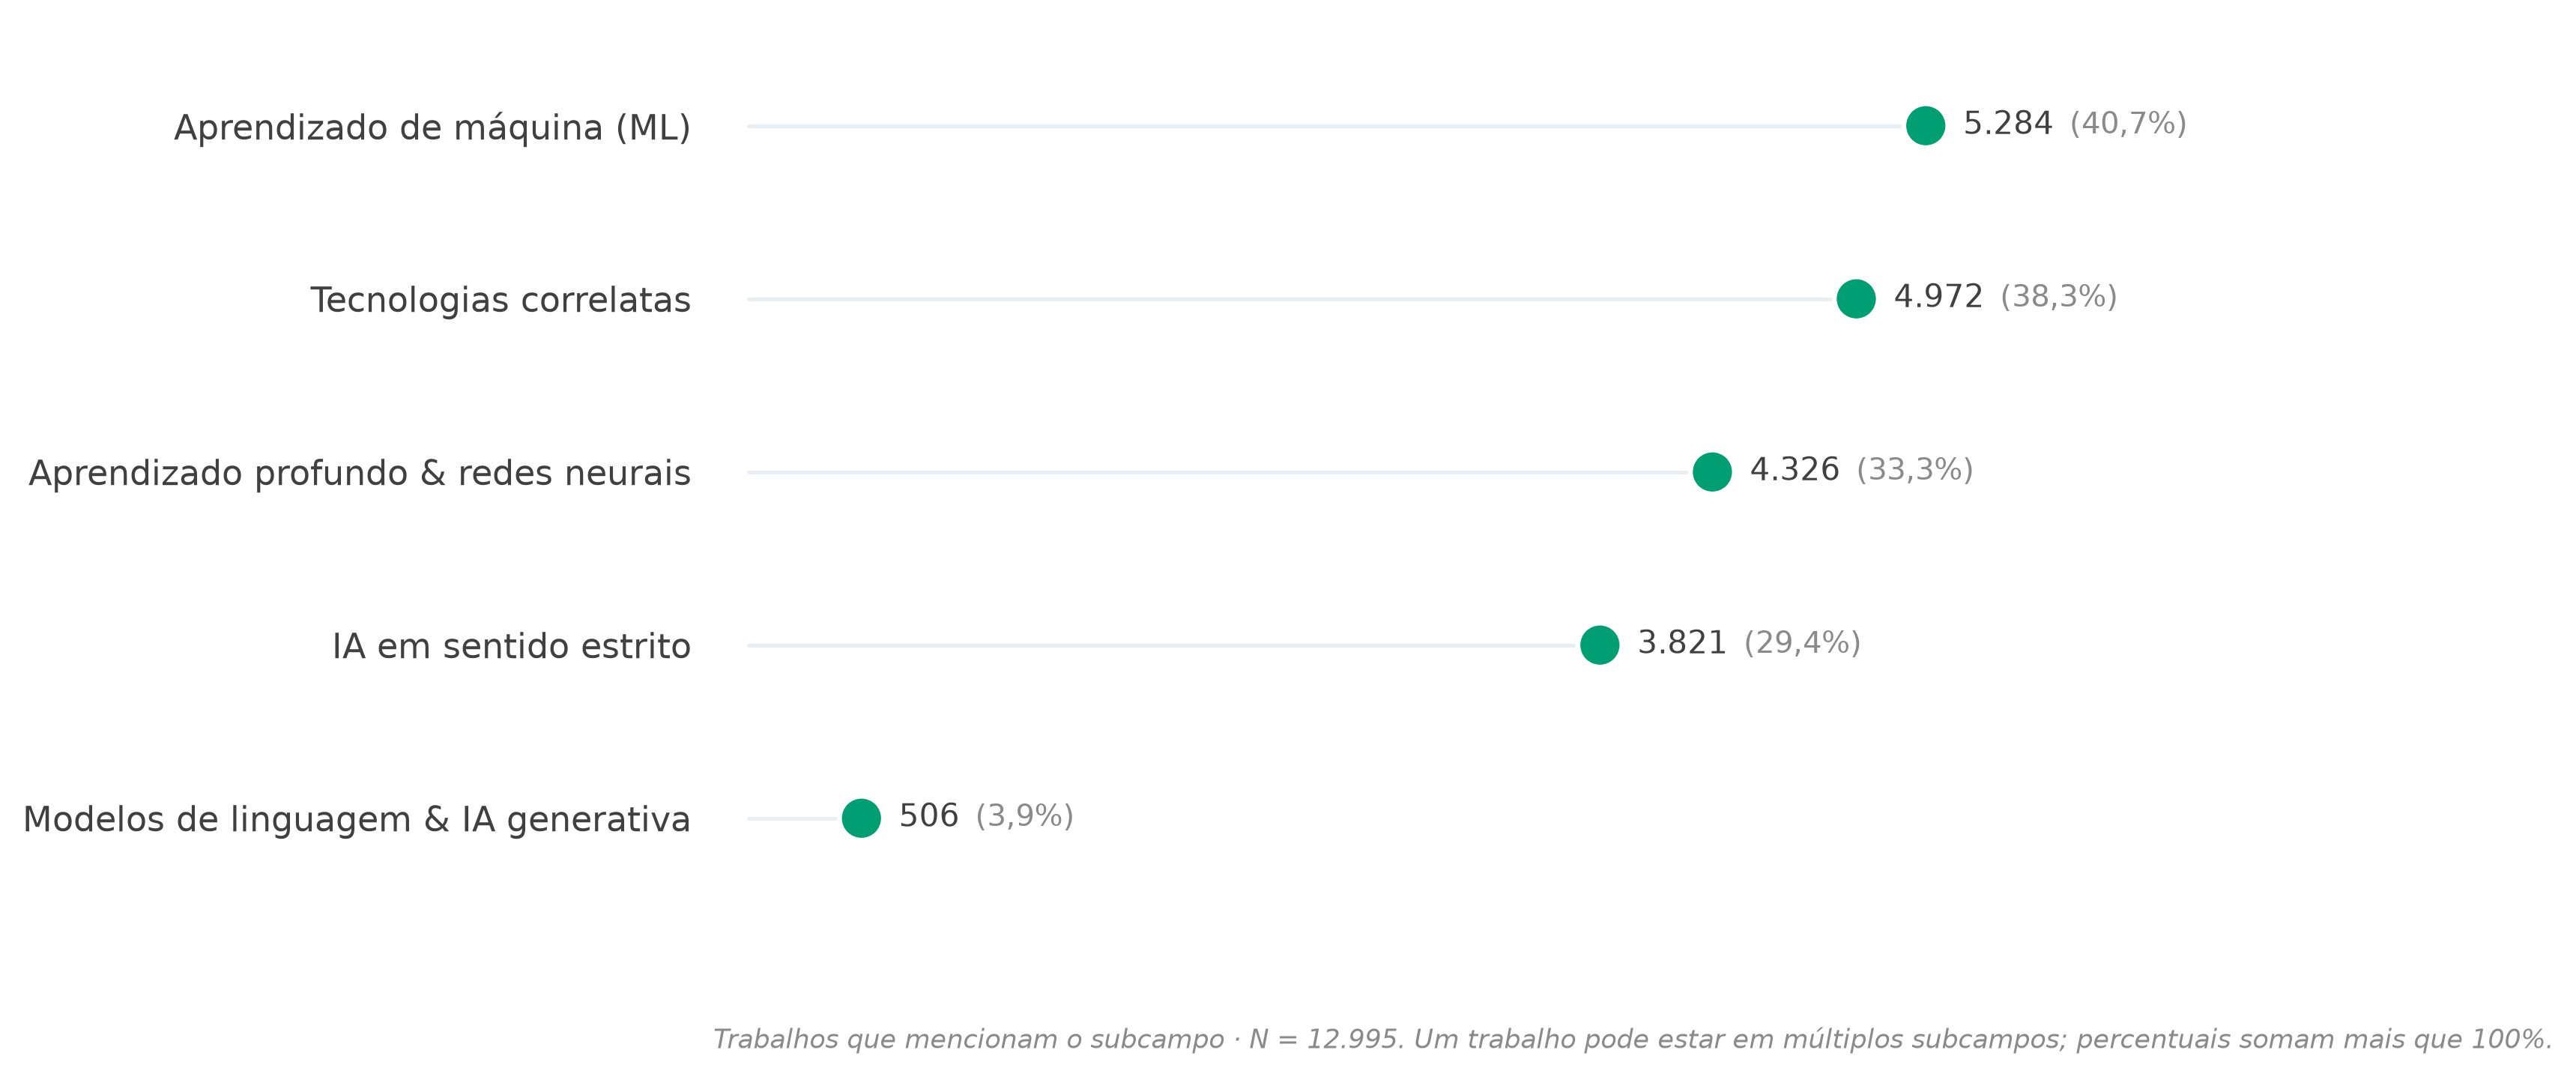
\includegraphics[width=0.85\linewidth]{figuras/cap.2/capes-scielo/capes_21_subcampos_distribuicao.png}
    \caption[Distribuição do corpus \texttt{Capes} por subcampo, 2021--2024]{%
        Distribuição das 12.995 defesas do corpus pelos cinco subcampos do
        classificador. Um mesmo trabalho pode pertencer a mais de um subcampo,
        e por isso a soma dos percentuais ultrapassa cem. O aprendizado de
        máquina é o subcampo mais frequente, com 5.284 defesas, seguido pelas
        tecnologias correlatas, com 4.972, e pelo aprendizado profundo e redes
        neurais, com 4.326, ao passo que a inteligência artificial em sentido
        estrito aparece só em quarto lugar, com 3.821, o que contraria
        a expectativa de que \enquote{inteligência artificial} seja o rótulo
        dominante. Os modelos de linguagem e a inteligência artificial
        generativa formam o menor subcampo em volume, com 506 defesas.
        Elaboração própria a partir do Catálogo de Teses e Dissertações da
        \texttt{Capes}, \emph{dump} oficial \texttt{BR-CAPES-BTD-2021A2024}.
        Dados de domínio público. Repositório com dados, \emph{scripts} e figuras em \protect\url{https://github.com/julianehelanski/bibliometria-ia-humanas}.}
    \label{fig:capes_subcampos}
\end{figure}

A distribuição dos cinco subcampos ao longo do quadriênio mostra um movimento que interessa de perto a esta tese. O aprendizado de máquina mantém-se como o subcampo de maior volume em todos os quatro anos, e os modelos de linguagem e a inteligência artificial generativa, embora sejam o menor subcampo em volume absoluto, apresentam o maior crescimento proporcional em 2024.\footnote{A figura que apresenta a evolução anual de cada um dos cinco subcampos no quadriênio fica versionada no repositório da análise bibliométrica, em \url{https://github.com/julianehelanski/bibliometria-ia-humanas}.} Esse salto é o corolário, na produção de pós-graduação brasileira, da popularização do \texttt{ChatGPT} a partir de novembro de 2022, e marca o momento em que a inteligência artificial generativa começa a ser absorvida como objeto de pesquisa pela pós-graduação do país.

Do universo de 350.071 trabalhos defendidos no quadriênio, 12.995 tocam o campo da inteligência artificial, do aprendizado de máquina ou do aprendizado profundo, o que corresponde a 3,71\% da produção nacional de pós-graduação. A Figura~\ref{fig:capes_grande_area} apresenta a distribuição desses 12.995 trabalhos pelas grandes áreas do conhecimento, e traz, além da participação de cada grande área no corpus de inteligência artificial, a taxa interna, isto é, o percentual da produção total de cada grande área que toca o campo.

\begin{figure}[htbp]
    \centering
    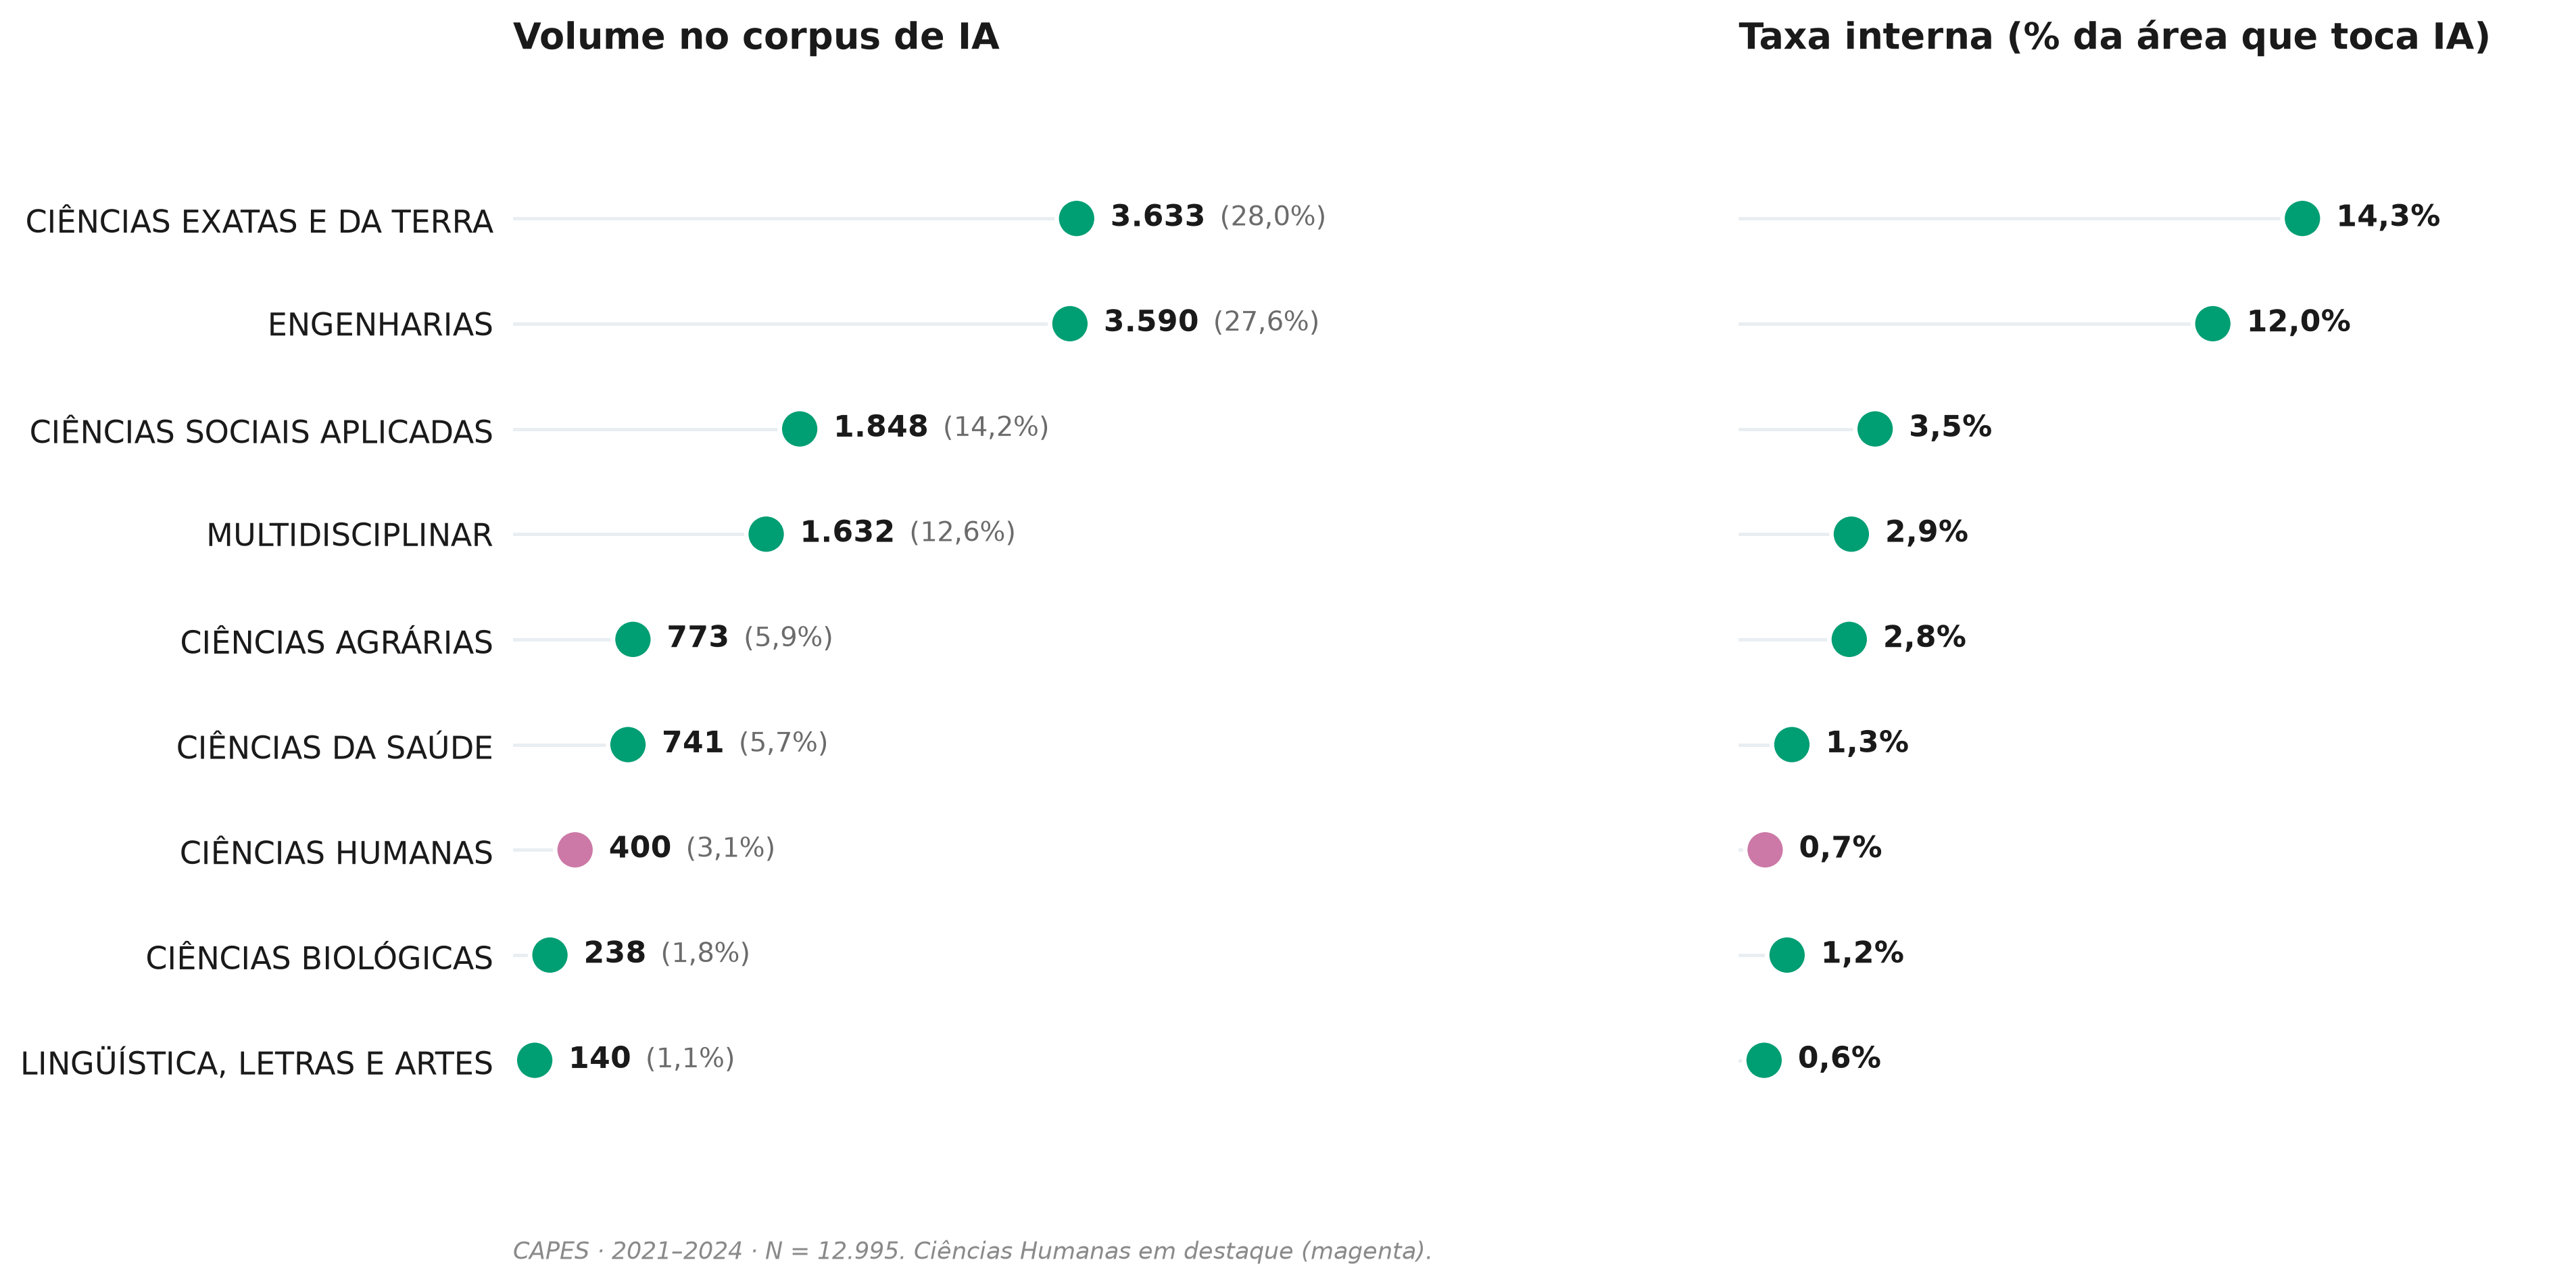
\includegraphics[width=0.95\linewidth]{figuras/cap.2/capes-scielo/capes_11_grande_area_share.png}
    \caption[Distribuição da produção sobre IA por grande área, \texttt{Capes} 2021--2024]{%
        Distribuição dos 12.995 trabalhos sobre inteligência artificial,
        aprendizado de máquina e aprendizado profundo defendidos na
        pós-graduação brasileira no quadriênio 2021--2024, por grande área de
        conhecimento. O painel da esquerda mostra o volume absoluto e a
        participação percentual no corpus, e o painel da direita mostra a taxa
        interna, isto é, a fração das defesas de cada grande área que tocam o
        campo. As Ciências Humanas, em destaque, são a maior grande área no
        universo total da pós-graduação brasileira, com 59.976 defesas no
        quadriênio, e ainda assim respondem por apenas 3,08\% do corpus de
        inteligência artificial, e somente 0,67\% das defesas em Ciências
        Humanas tocam o campo, contra 14,29\% nas Ciências Exatas e da Terra e
        12,01\% nas Engenharias. Elaboração própria a partir do Catálogo de
        Teses e Dissertações da \texttt{Capes}, \emph{dump} oficial
        \texttt{BR-CAPES-BTD-2021A2024}. Dados de domínio público. Repositório com dados, \emph{scripts} e figuras em \protect\url{https://github.com/julianehelanski/bibliometria-ia-humanas}.}
    \label{fig:capes_grande_area}
\end{figure}

A Figura~\ref{fig:capes_grande_area} permite ler a posição das Ciências Humanas em dois modos. No primeiro, as Ciências Humanas são a maior grande área do universo total da pós-graduação brasileira, com 59.976 trabalhos defendidos no quadriênio, e contribuem com apenas 3,08\% do corpus de inteligência artificial. No segundo, e a leitura que mais pesa para o argumento, apenas 0,67\% das defesas em Ciências Humanas tocam o campo da inteligência artificial, contra 12,01\% nas Engenharias e 14,29\% nas Ciências Exatas e da Terra, uma diferença de uma ordem de grandeza. As ciências humanas brasileiras se aproximam da inteligência artificial como objeto de pesquisa em um ritmo que é, em termos proporcionais, entre dezoito e vinte e uma vezes mais lento que o das engenharias e das ciências exatas.

A diferença entre as grandes áreas é de volume e de vocabulário. Quando cruzo os cinco subcampos com as nove grandes áreas, encontro o que chamo de assinatura discursiva de cada área, isto é, o conjunto de termos pelos quais cada grande área se aproxima do campo. O aprendizado profundo e as redes neurais concentram-se de modo quase exclusivo nas Ciências Exatas e nas Engenharias, e as Ciências Humanas, quando tocam o campo, tocam-no sobretudo pela inteligência artificial como conceito e pelas tecnologias correlatas, e quase nunca pelos termos técnicos. As Figuras~\ref{fig:capes_heatmap_keyword} e~\ref{fig:capes_heatmap_subcampo} apresentam esse cruzamento em dois recortes. A leitura das duas figuras sustenta um ponto que importa ao argumento desta tese: a inteligência artificial significa coisas distintas em áreas distintas, mesmo quando a soma agregada parece uniforme, e os modelos de linguagem e a inteligência artificial generativa são o subcampo que mais atravessa as fronteiras disciplinares, com presença que se espalha pelas Ciências Sociais Aplicadas, pela área Multidisciplinar e pelas Ciências Humanas, em lugar de se concentrar nas exatas. Quando uma defesa fora das ciências exatas toca o campo, é mais provável que o faça pela porta da inteligência artificial generativa do que pela das redes neurais, e esse achado é coerente com a hipótese que sustento sobre o \texttt{ChatGPT} como ponto de virada da entrada da inteligência artificial no discurso público e nas ciências humanas.

\begin{figure}[htbp]
    \centering
    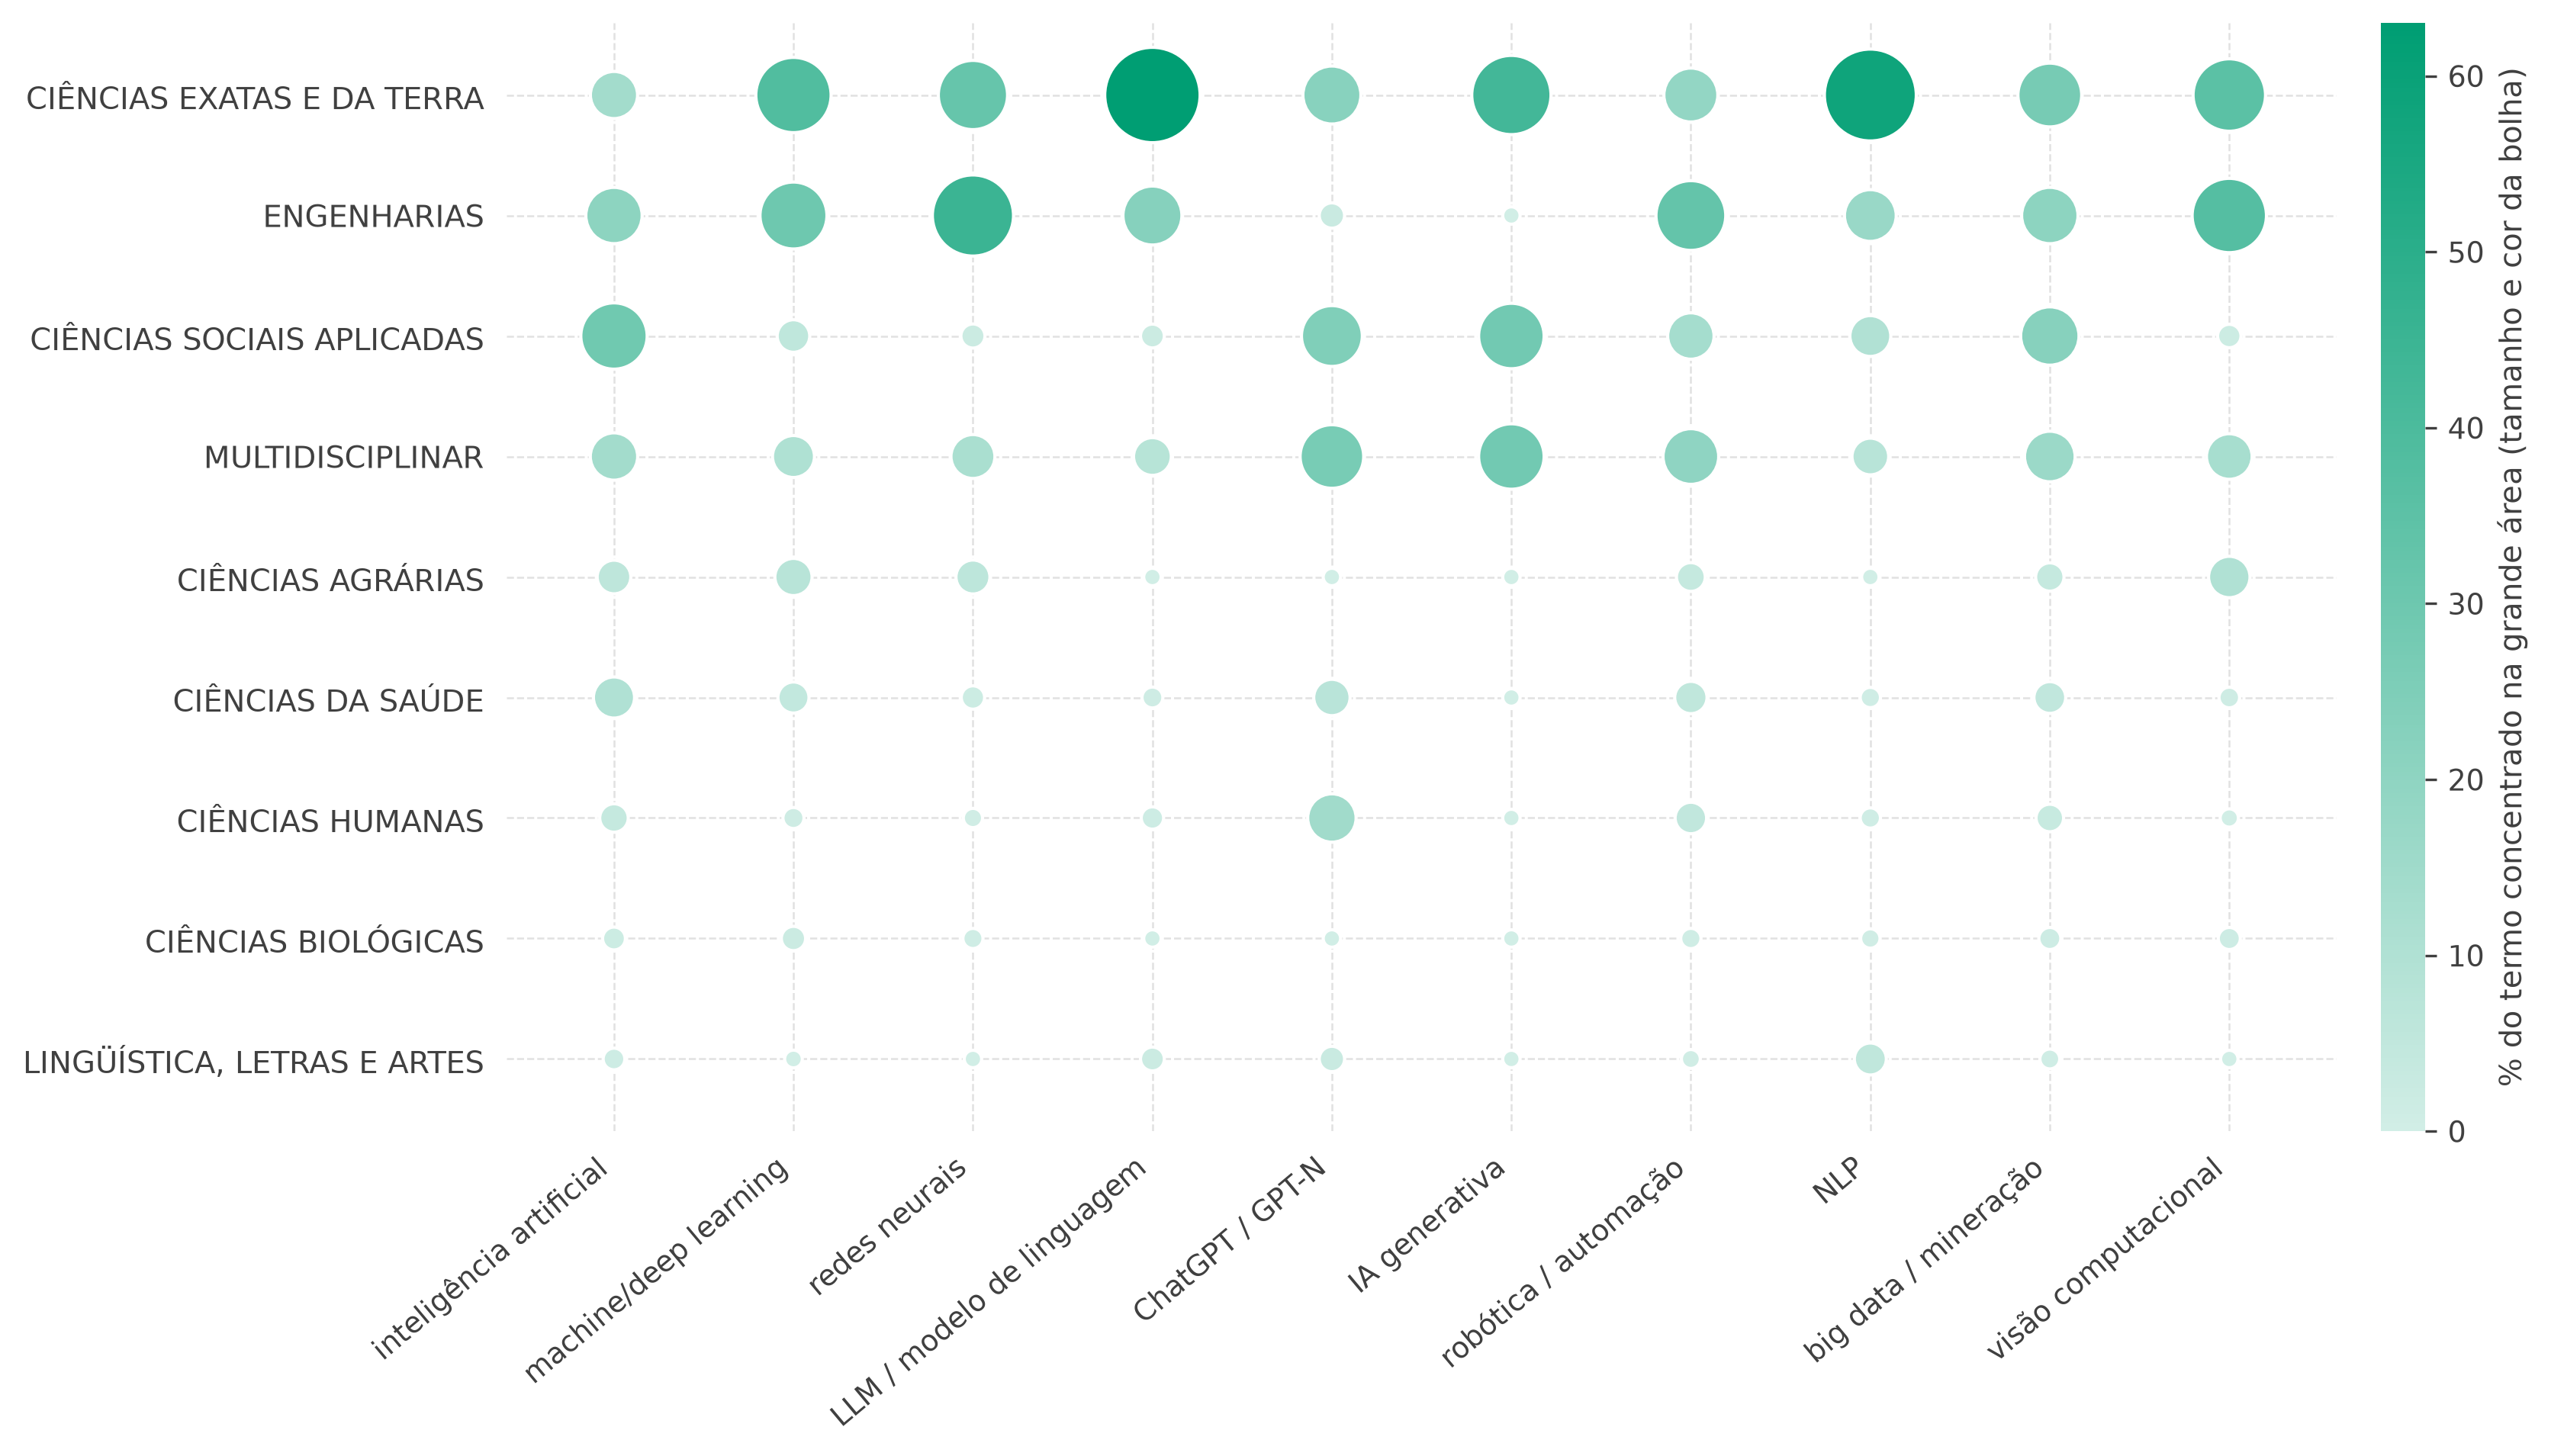
\includegraphics[width=0.95\linewidth]{figuras/cap.2/capes-scielo/capes_13_heatmap_area_keyword.png}
       \caption[Co-ocorrência entre termos-chave e grandes áreas, \texttt{Capes} 2021--2024]{%
        Matriz de bolhas da co-ocorrência entre dez termos-chave do campo e as
        nove grandes áreas de conhecimento da \texttt{Capes}, sobre o corpus de
        12.995 defesas. Em cada cruzamento, o tamanho e a cor da bolha indicam o
        percentual do termo da coluna que se concentra naquela grande área, numa
        escala sequencial branco-verde ancorada no verde Okabe-Ito, em matiz
        distinto do par azul-vermelho das matrizes de bolhas do
        capítulo~\ref{capitulo3}, segundo a colorbar à direita da figura. A
        leitura por coluna evidencia que termos como \enquote{redes neurais} e
        \enquote{aprendizado profundo} concentram-se nas Ciências Exatas e nas
        Engenharias, ao passo que \enquote{\texttt{ChatGPT}} distribui-se por
        todas as áreas, com presença nas Ciências Sociais Aplicadas e nas
        Ciências Humanas. Elaboração própria a partir do Catálogo de Teses e
        Dissertações da \texttt{Capes}, \emph{dump} oficial
        \texttt{BR-CAPES-BTD-2021A2024}. Dados de domínio público. Repositório
        com dados, \emph{scripts} e figuras em
        \protect\url{https://github.com/julianehelanski/bibliometria-ia-humanas}.}
    \label{fig:capes_heatmap_keyword}
\end{figure}

\begin{figure}[htbp]
    \centering
    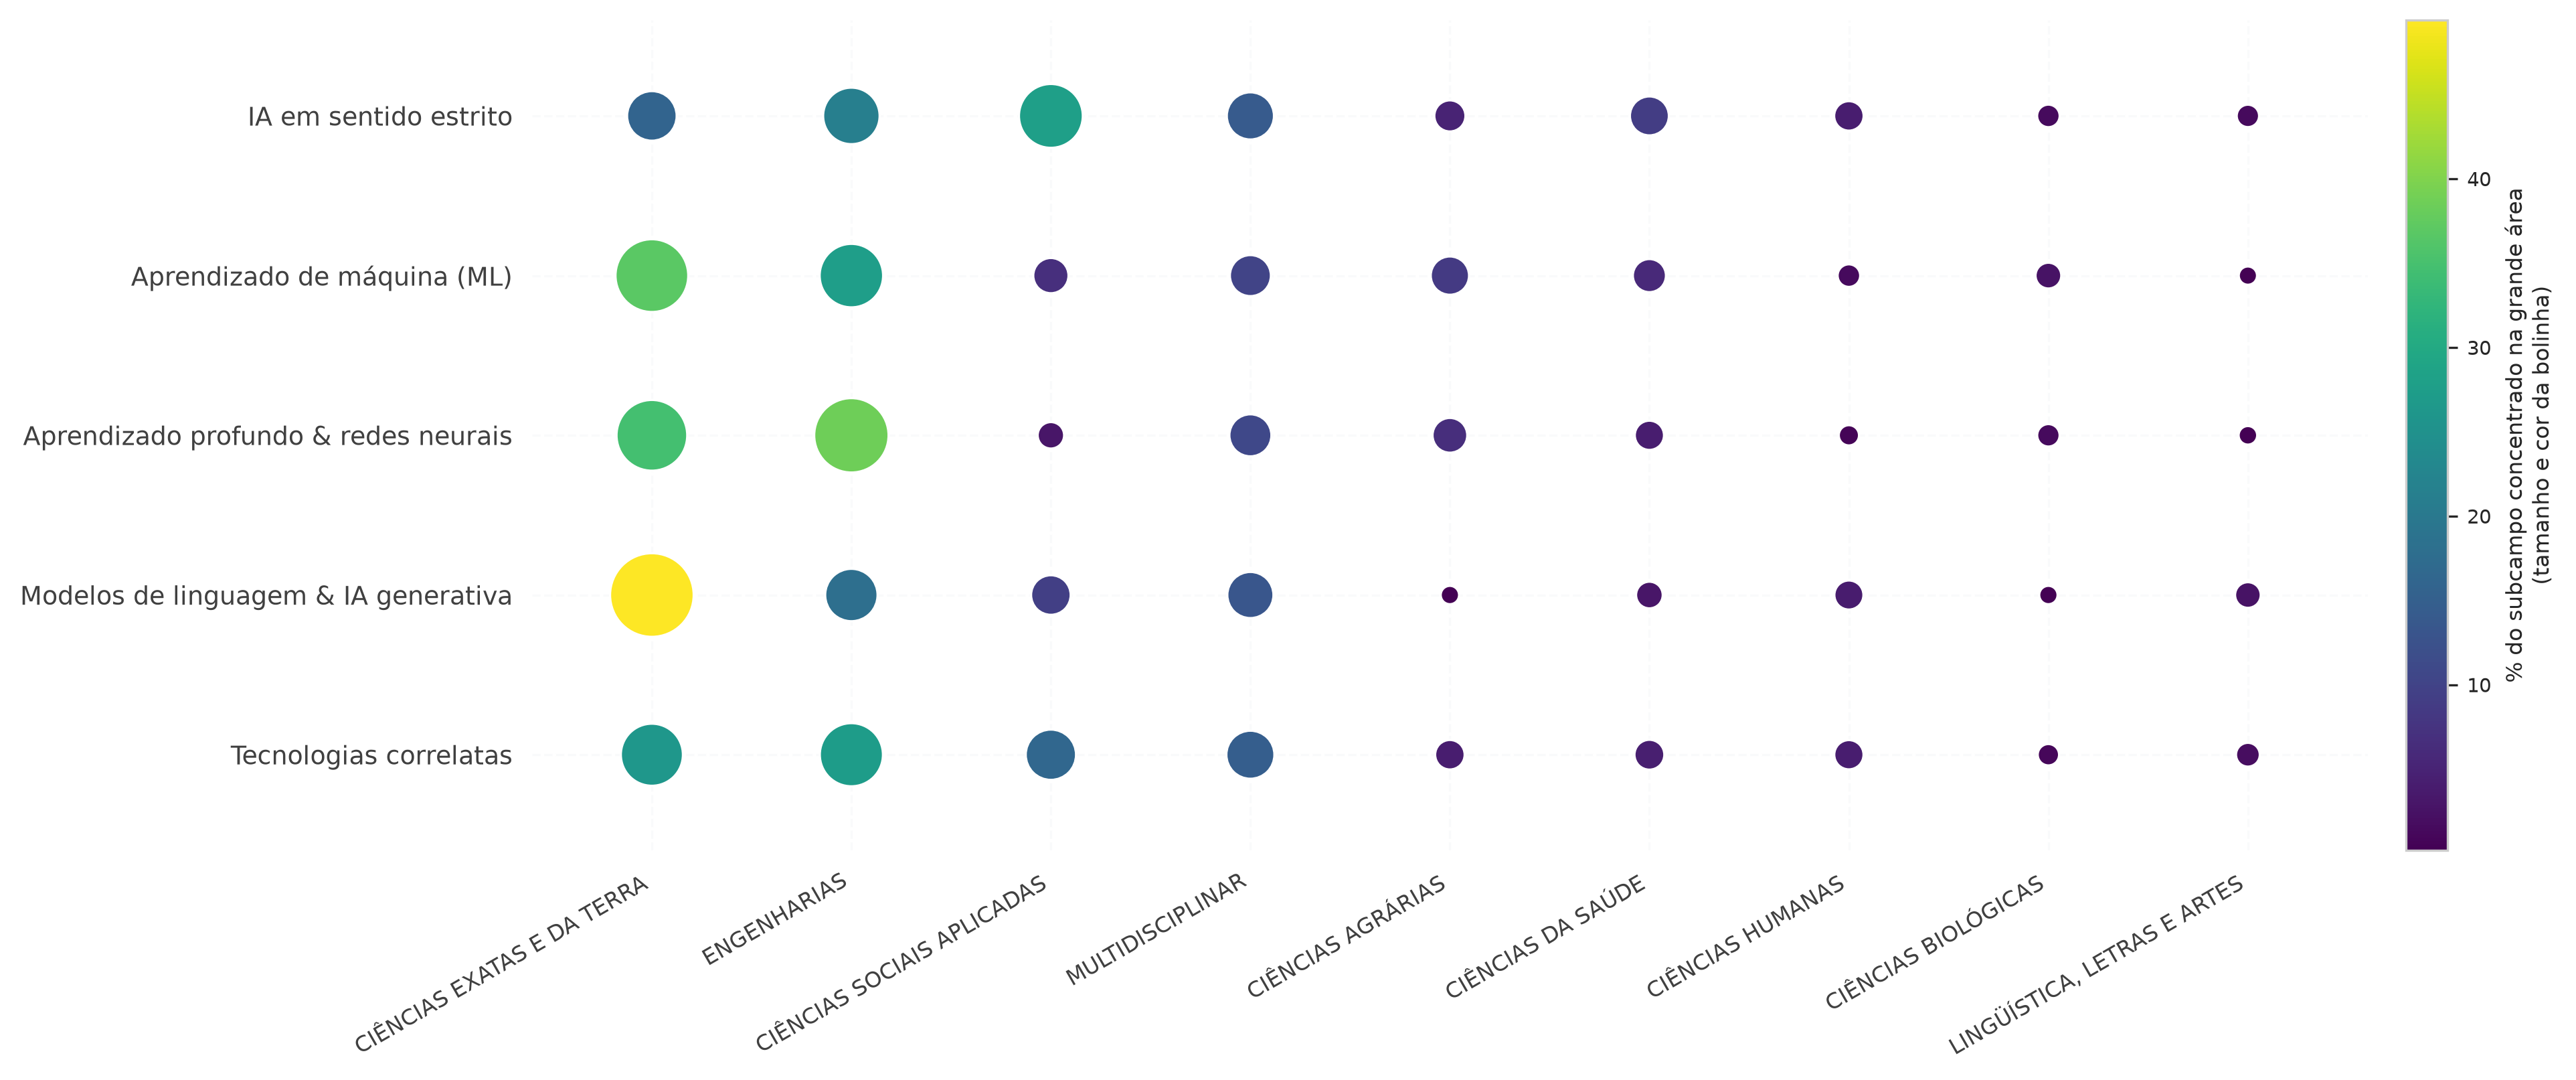
\includegraphics[width=0.95\linewidth]{figuras/cap.2/capes-scielo/capes_22_heatmap_subcampo_grande_area.png}
        \caption[Concentração dos subcampos por grande área, \texttt{Capes} 2021--2024]{%
        Matriz de bolhas da concentração dos cinco subcampos do classificador
        entre as nove grandes áreas. Cada linha, que corresponde a um subcampo,
        está normalizada para somar cem por cento, e mostra, para cada técnica,
        onde ela se concentra. Em cada cruzamento, o tamanho e a cor da bolha
        indicam o percentual do subcampo distribuído naquela grande área, numa
        escala sequencial branco-laranja ancorada no laranja Okabe-Ito, em
        matiz distinto do verde da Figura~\ref{fig:capes_heatmap_keyword} e
        do par azul-vermelho das matrizes de bolhas do
        capítulo~\ref{capitulo3}, segundo a colorbar à direita da figura. O
        aprendizado profundo e as redes neurais concentram-se nas Ciências
        Exatas e nas Engenharias, e os modelos de linguagem e a inteligência
        artificial generativa distribuem-se de modo mais espalhado, com
        presença nas Ciências Sociais Aplicadas, na área Multidisciplinar e
        nas Ciências Humanas. Elaboração própria a partir do Catálogo de Teses
        e Dissertações da \texttt{Capes}, \emph{dump} oficial
        \texttt{BR-CAPES-BTD-2021A2024}. Dados de domínio público. Repositório
        com dados, \emph{scripts} e figuras em
        \protect\url{https://github.com/julianehelanski/bibliometria-ia-humanas}.}
    \label{fig:capes_heatmap_subcampo}
\end{figure}

Os 400 trabalhos das Ciências Humanas que tocam o campo distribuem-se de modo desigual pelas áreas de conhecimento da grande área. A Figura~\ref{fig:capes_humanas_area} apresenta essa distribuição.

\begin{figure}[htbp]
    \centering
    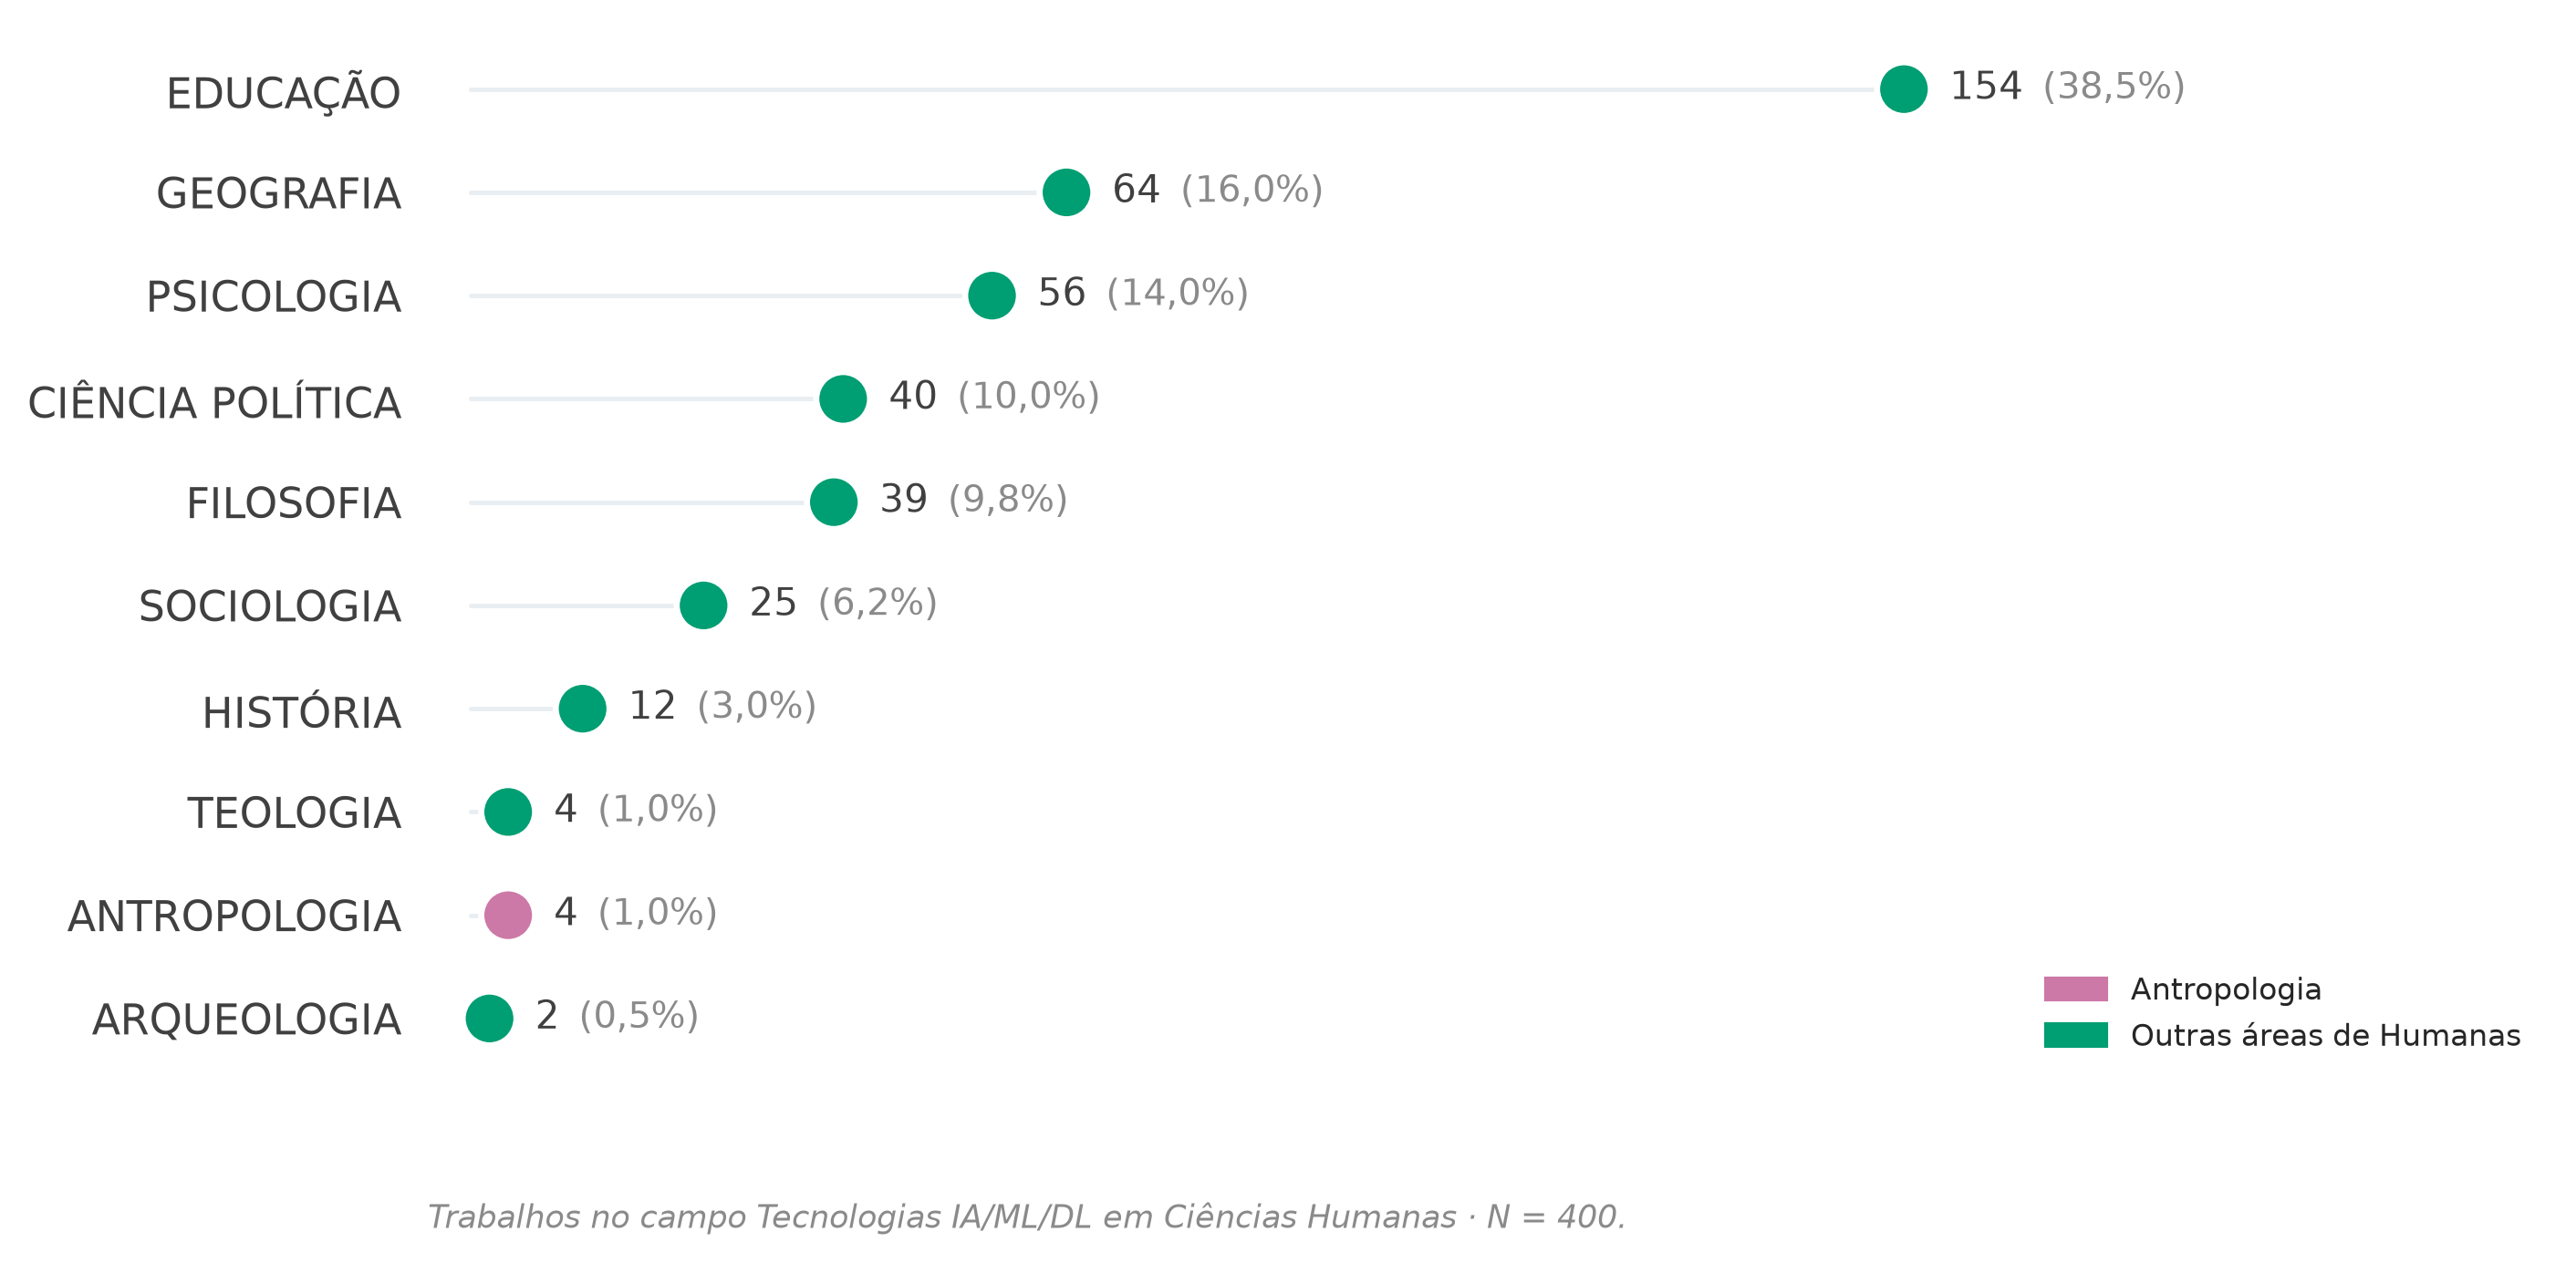
\includegraphics[width=0.85\linewidth]{figuras/cap.2/capes-scielo/capes_h01_areas_humanas.png}
    \caption[Produção sobre IA nas Ciências Humanas por área, \texttt{Capes} 2021--2024]{%
        Distribuição das 400 defesas sobre inteligência artificial, aprendizado
        de máquina e aprendizado profundo na grande área de Ciências Humanas
        (2021--2024), por área de conhecimento. A Educação responde por 38,5\%
        das defesas, e é seguida de longe pela Geografia, com 16,0\%, e pela
        Psicologia, com 14,0\%. A Antropologia, em destaque, aparece com quatro
        defesas, 1,0\% do total, e ocupa a penúltima posição, à frente apenas
        da Arqueologia. A figura permite ler a marginalidade da Antropologia em
        duas camadas: a inteligência artificial é objeto periférico dentro das
        Ciências Humanas, e a Antropologia é periférica dentro desse recorte já
        periférico. Elaboração própria a partir do Catálogo de Teses e
        Dissertações da \texttt{Capes}, \emph{dump} oficial
        \texttt{BR-CAPES-BTD-2021A2024}. Dados de domínio público. Repositório com dados, \emph{scripts} e figuras em \protect\url{https://github.com/julianehelanski/bibliometria-ia-humanas}.}
    \label{fig:capes_humanas_area}
\end{figure}

A Educação concentra 38,5\% da produção de inteligência artificial em Ciências Humanas, e é seguida de longe pela Geografia e pela Psicologia. As três disciplinas que compõem o que costumo chamar de ciências sociais em sentido estrito, a Ciência Política, a Sociologia e a Antropologia, somam 69 das 400 defesas. A Antropologia registra quatro defesas sobre inteligência artificial no quadriênio 2021--2024 pela área de conhecimento da \texttt{Capes}; pela taxonomia de avaliação da agência, que agrupa Antropologia e Arqueologia em uma única área administrativa, são seis defesas.\footnote{A \texttt{Capes} classifica cada trabalho por dois critérios distintos, registrados em colunas separadas do \emph{dump} oficial. A área de conhecimento (\texttt{NM\_AREA\_CONHECIMENTO}) é o recorte disciplinar estrito, e nela a Antropologia tem quatro defesas e a Arqueologia tem duas. A área de avaliação (\texttt{NM\_AREA\_AVALIACAO}) é o recorte do organograma administrativo, pelo qual os programas de pós-graduação são de fato agrupados pela agência, e nela Antropologia e Arqueologia formam uma única área com seis defesas. Adoto os dois números porque a marginalidade que descrevo independe do critério: quatro ou seis, frente às 154 defesas da Educação ou às 64 da Geografia, sustentam a mesma leitura. As contagens das duas colunas, lidas diretamente da planilha, fecham em 400 em ambos os recortes, e ficam versionadas no arquivo \texttt{docs/decisoes\_metodologicas.md} do repositório.} Pela área de conhecimento, a Antropologia é a penúltima da figura, à frente apenas da Arqueologia. A posição da Antropologia se lê, assim, em camadas: a inteligência artificial é marginal no conjunto das Ciências Humanas, com 0,67\% da produção da grande área, e a Antropologia é marginal dentro desse conjunto já marginal, com 1,0\% das 400 defesas de inteligência artificial em Ciências Humanas. Quatro trabalhos em quatro anos, frente aos 154 da Educação ou aos 64 da Geografia, é uma densidade que situa minha tese no início dos estudos antropológicos brasileiros sobre inteligência artificial.

Na Antropologia, quatro defesas em quatro anos é pouco, e, ao ler caso a caso, verifico que esses quatro trabalhos, retornados pela classificação automática, não correspondem a quatro etnografias da inteligência artificial em específico. Das quatro defesas, duas tomam a inteligência artificial como objeto etnográfico em sentido estrito. A dissertação de Rafael Damasceno Ramalho Pereira, \textit{O problema das outras mentes: uma antropologia das inteligências artificiais}, defendida na \texttt{UFRJ} em 2021 sob orientação de Eduardo Viveiros de Castro, coloca o problema da simulação da mente diante do conceito antropológico de cultura para constituir o campo de uma antropologia das inteligências artificiais, e busca um caminho que escape tanto ao cognitivismo das ciências exatas quanto à genealogia do poder das ciências sociais, com a conclusão de que as concepções de inteligência que respaldam esses projetos vêm acopladas a uma despolitização do espírito. A dissertação de Louise Lima Karczeski, \textit{Gerando inteligência: considerações etnográficas sobre a construção de objetividade no campo da inteligência artificial}, defendida na \texttt{UFSC} em 2022 sob orientação de Leticia Cesarino, acompanha em conferências, cursos e comunidades on-line os especialistas que elaboram modelos de inteligência artificial, e descreve como eles reivindicam a objetividade de suas aplicações por três enquadres, o mercado, a ciência e a ética; é, das quatro, a mais próxima do que faço nesta tese. As outras duas defesas tocam o campo de modo oblíquo: a tese de Isabel Wittmann, \textit{Feminilidades maquínicas: gênero, sexualidade e corpo de mulheres artificiais no cinema fantástico}, defendida na \texttt{USP} em 2023 sob orientação de Rose Satiko Gitirana Hikiji, traça uma genealogia das mulheres artificiais no cinema, de \textit{Metrópolis} a \textit{Ex Machina}, e aciona androides, robôs e ciborgues como figuras culturais à luz das teóricas feministas do cinema, em lugar de tomar um sistema técnico como objeto; e a dissertação de Fabricio Bernardes, \textit{Gerenciamento de dados arqueológicos digitais: estudo de caso a partir da região estuarina do município de Rio Grande, Rio Grande do Sul, Brasil}, defendida na \texttt{UFPel} em 2023 sob orientação de Rafael Guedes Milheira, avalia a curadoria e o reaproveitamento dos dados arqueológicos do \texttt{IPHAN} pelos conceitos de inventário patrimonial, ciberinfraestrutura e \emph{big data}, e foi retornada pelo classificador por tocar o subcampo das tecnologias correlatas, sem ser uma pesquisa sobre inteligência artificial. A distância entre os quatro trabalhos retornados pelo classificador e as duas etnografias que de fato tomam a inteligência artificial como objeto é o tipo de distinção que a classificação automática não faz, e que a leitura situada precisa fazer.\footnote{A triagem de auditoria é a leitura caso a caso que faço sobre o resultado do \emph{regex} de cinco subcampos em cada recorte disciplinar, e o seu princípio vale para além do caso da Antropologia. O \emph{regex} detecta a presença de um termo, e não o uso que o trabalho faz dele, e por isso gera dois tipos de falso positivo. O primeiro é o trabalho que menciona um termo do campo como contexto ou horizonte, sem que a inteligência artificial seja seu objeto. O segundo é o trabalho que aplica uma técnica de aprendizado de máquina como método, em que a inteligência artificial entra como instrumento e não como objeto da pesquisa, como nas defesas de Ciência Política que preveem a qualidade de medicamentos ou recomendam ações parlamentares. A planilha de auditoria por registro, com a classificação de cada trabalho, fica versionada no repositório para conferência e discussão.}

A Sociologia e a Ciência Política aparecem ao campo em número maior que a Antropologia, com 25 e 40 defesas respectivamente, e, ao ler os dois conjuntos, identifico que cada disciplina se aproxima da inteligência artificial por caminhos próprios. Na Sociologia, das 25 defesas, dezesseis tocam o subcampo das tecnologias correlatas, e o conjunto se organiza em boa parte em torno de temas como trabalho, plataformas e datificação. Entre esses temas, objetos de pesquisa como a automação na indústria farmacêutica de Anápolis, a automação do atendimento nos supermercados de Fortaleza, a reestruturação do trabalho bancário, o trabalho de entregadores por aplicativo no capitalismo de plataforma, o teletrabalho no \texttt{INSS} durante a pandemia, a transição das estatísticas oficiais para um regime de dataficação. Outras defesas desse subconjunto seguem para as redes sociais e a circulação de dados em chave política, com estudos sobre a \enquote{fala do crime} no Facebook, os grupos bolsonaristas no WhatsApp, o \emph{big data} no 7 de setembro de 2021 e o uso de tecnologias emergentes pelas forças de segurança do Ceará, ao lado de entradas mais dispersas sobre tecnologia espacial e o \texttt{INPE}, o mercado de automóveis, os \emph{chatbots} no contexto comercial e o patrocínio empresarial na arte contemporânea. A inteligência artificial aparece à Sociologia brasileira no contexto da transformação do trabalho e do mundo digital. Um caso destoa do conjunto e interessa a esta tese, a dissertação de João Ricardo Penteado Lopes da Silva, \textit{Tendências das políticas do Estado brasileiro para o desenvolvimento da inteligência artificial: o caso dos centros de pesquisa aplicada em inteligência artificial}, defendida na \texttt{UFC} em 2022 sob orientação de Edemilson Cruz Santana Junior, toma como objeto centros de pesquisa aplicada como o \texttt{C4AI}. Na Ciência Política e nas Relações Internacionais, das 40 defesas, um primeiro conjunto se organiza em torno da geopolítica, da defesa e da segurança, e varia entre temas como a competição estratégica entre Estados Unidos e China pela liderança em inteligência artificial, a disputa em torno da Huawei e do 5G, os drones e as embarcações autônomas, a guerra cognitiva nas redes sociais, e também temas como \emph{big data} no policiamento da Polícia Militar de Minas Gerais. Um segundo conjunto vem da administração pública e do poder legislativo, e parte da inteligência artificial na gestão estatal, como a inteligência artificial no judiciário e na gestão de acervo processual, na avaliação de políticas públicas, no combate ao sobrepreço nas compras públicas, na regulação das consultas normativas da Anatel e na comunicação política dos senadores nas redes. Uma parte dessas defesas, ademais, não toma a inteligência artificial por objeto, e a usa como método de análise por aprendizado de máquina, em temas mais específicos como a predição da qualidade de medicamentos e a recomendação de ações parlamentares e de padrões de carreira parlamentar.

A distribuição temporal dos 400 trabalhos de inteligência artificial em Ciências Humanas mostra uma curva de aceleração: 69 defesas em 2021, 81 em 2022, 108 em 2023 e 142 em 2024. A produção mais que dobrou no intervalo de quatro anos, e a aceleração é coerente com a popularização da inteligência artificial generativa a partir do final de 2022. A Figura~\ref{fig:capes_temporal} apresenta essa curva.

\begin{figure}[htbp]
    \centering
    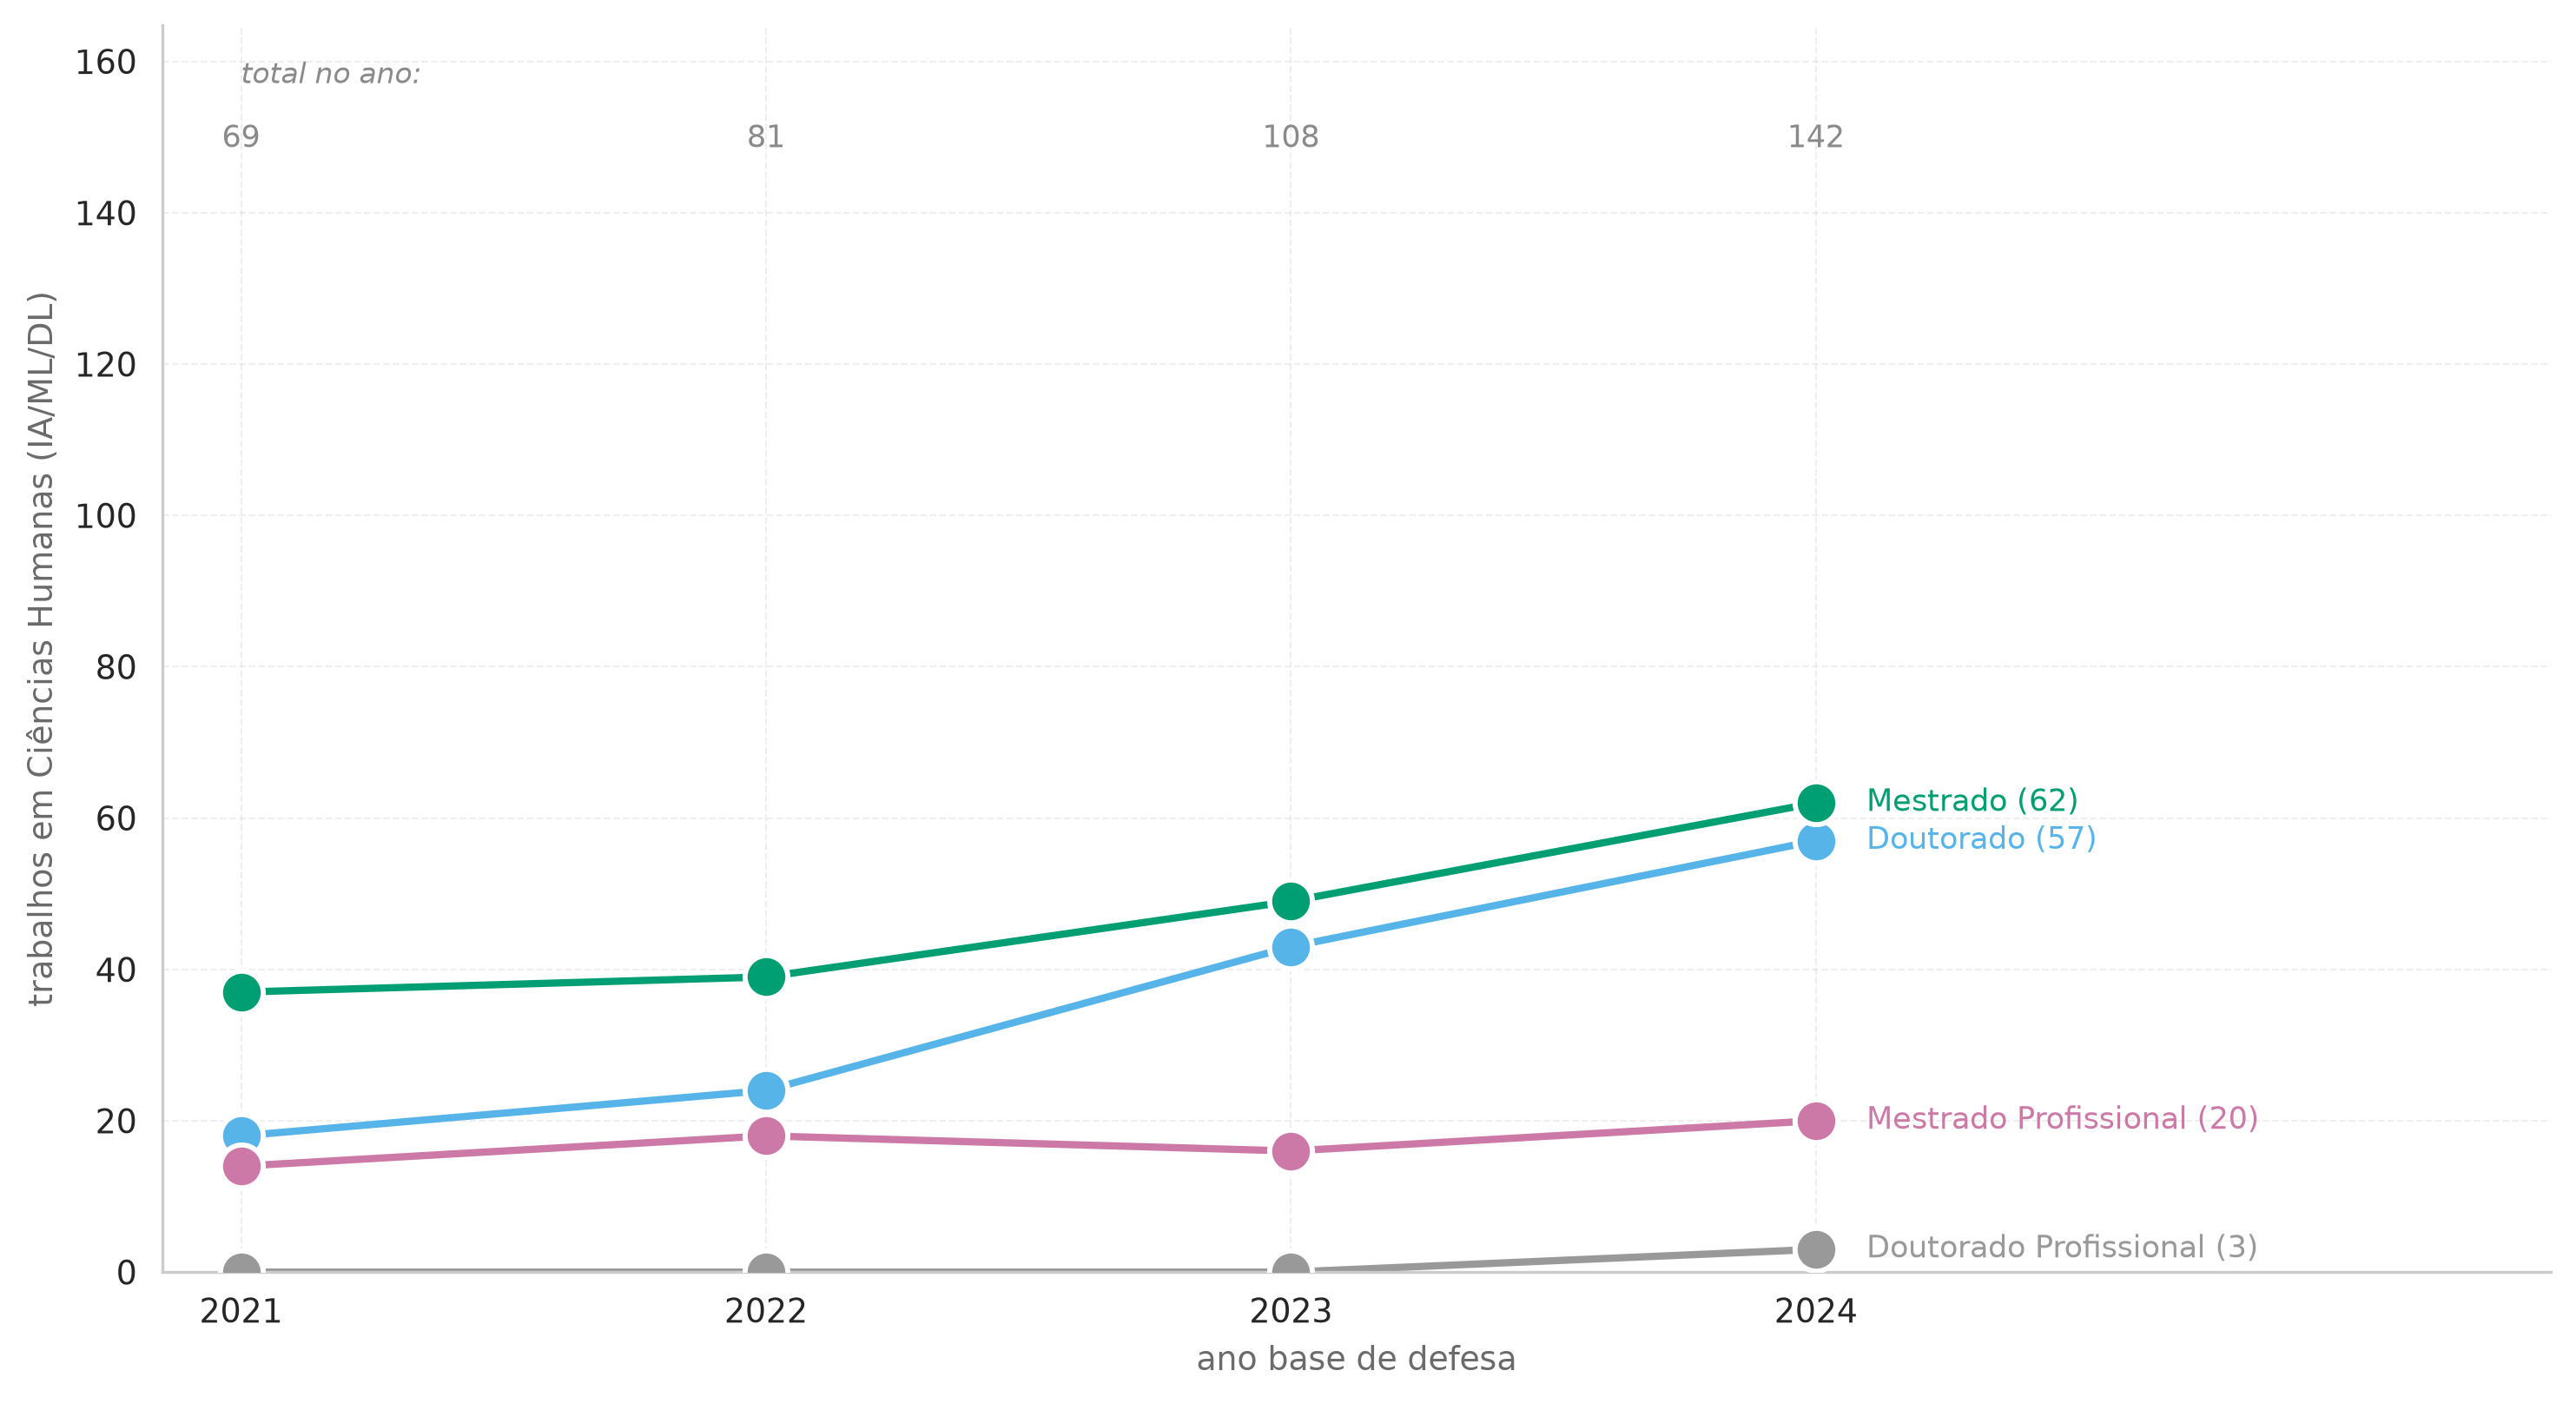
\includegraphics[width=0.85\linewidth]{figuras/cap.2/capes-scielo/capes_h02_temporal_humanas.png}
    \caption[Evolução temporal da produção sobre IA nas Ciências Humanas, \texttt{Capes} 2021--2024]{%
        Evolução anual das defesas em Ciências Humanas no campo da inteligência
        artificial, do aprendizado de máquina e do aprendizado profundo
        (2021--2024), em uma linha por grau acadêmico. O conjunto cresce de 69
        defesas em 2021 para 142 em 2024, mais que o dobro no intervalo de
        quatro anos, e o Mestrado responde pela maior parte do crescimento. A
        curva indica que as Ciências Humanas se aproximam do campo a partir de
        uma base reduzida, e que a marginalidade que descrevo é o estado
        presente de um campo em formação, em lugar de uma tendência estática.
        Elaboração própria a partir do Catálogo de Teses e Dissertações da
        \texttt{Capes}, \emph{dump} oficial \texttt{BR-CAPES-BTD-2021A2024}.
        Dados de domínio público. Repositório com dados, \emph{scripts} e figuras em \protect\url{https://github.com/julianehelanski/bibliometria-ia-humanas}.}
    \label{fig:capes_temporal}
\end{figure}

A segunda base do mapeamento é a coleção brasileira da biblioteca eletrônica \texttt{SciELO}, que indexa o artigo publicado em periódico. Coletei o corpus \texttt{SciELO} pela \emph{API} ArticleMeta. Uma \emph{API} (\emph{Application Programming Interface}, ou interface de programação de aplicações) é um canal pelo qual um sistema disponibiliza seus dados de modo estruturado, para que outro programa os requisite de forma automatizada, em lugar da navegação manual pela página \emph{web}. No caso da \texttt{SciELO}, a \emph{API} ArticleMeta devolve os metadados de cada artigo da coleção, como título, autoria, ano, periódico e área, em formato legível por máquina, e foi por ela que requisitei o corpus.\footnote{A \emph{API} ArticleMeta é o serviço de acesso programático aos metadados da rede \texttt{SciELO}, mantido pela própria plataforma. Requisitei o corpus com o \texttt{claude code} no terminal, em sessões iteradas de requisição, classificação e auditoria, e versionei o \emph{cache} completo da coleta no repositório. A \emph{API} delimita a janela temporal pela data de indexação do artigo na plataforma, e não pela data de publicação, e por isso a coleta bruta retornou artigos fora do quadriênio: dos 659 artigos no campo da inteligência artificial retornados sem filtro de ano, 28 foram publicados fora de 2021--2024 e ficam descartados de todas as análises desta seção. Os dados da \texttt{SciELO} são dinâmicos, e consultas futuras podem apresentar resultados distintos. Os números canônicos das duas bases, e a proveniência de cada um, ficam versionados no arquivo \texttt{docs/decisoes\_metodologicas.md} do repositório.} A coleta bruta retornou 98.165 artigos da coleção brasileira, e o recorte estrito ao quadriênio 2021--2024, por ano de publicação, delimita o universo de 90.360 artigos sobre o qual calculo as taxas internas. Apliquei a esse universo o mesmo \emph{regex} de cinco subcampos que apliquei ao Catálogo da \texttt{Capes}, e o classificador identificou 631 artigos no campo da inteligência artificial, do aprendizado de máquina e do aprendizado profundo. Dos 631 artigos do recorte, 225 foram publicados em 2024 contra 107 em 2021, crescimento que registra, na produção publicada em periódico, a mesma aceleração recente que a \texttt{Capes} mostra na produção de pós-graduação.

A Figura~\ref{fig:scielo_subject_area} apresenta a distribuição dos 631 artigos pelas oito \emph{subject\_areas} da coleção, mais a categoria Multidisciplinar que reúne os periódicos de classificação múltipla, com a taxa interna de cada uma.\footnote{O \texttt{SciELO} classifica seus periódicos em oito \emph{subject\_areas} canônicas. A categoria Multidisciplinar não é uma delas: agrupa os periódicos cuja classificação lista mais de uma área, e a mantenho como categoria sintética do meu procedimento de classificação. A taxa interna de uma área é a fração dos artigos dessa área que tocam o campo da inteligência artificial, isto é, o número de artigos da área no campo dividido pelo total de artigos que a área publicou no quadriênio. Por usar como base o universo de cada área, e não o volume absoluto, a taxa interna permite comparar a densidade do tema entre áreas de tamanhos distintos: a Engenharia publica menos que as Ciências da Saúde em número absoluto de artigos sobre inteligência artificial, e ainda assim apresenta a maior taxa interna, porque a inteligência artificial ocupa uma fração maior do que a Engenharia publica.}

\begin{figure}[htbp]
    \centering
    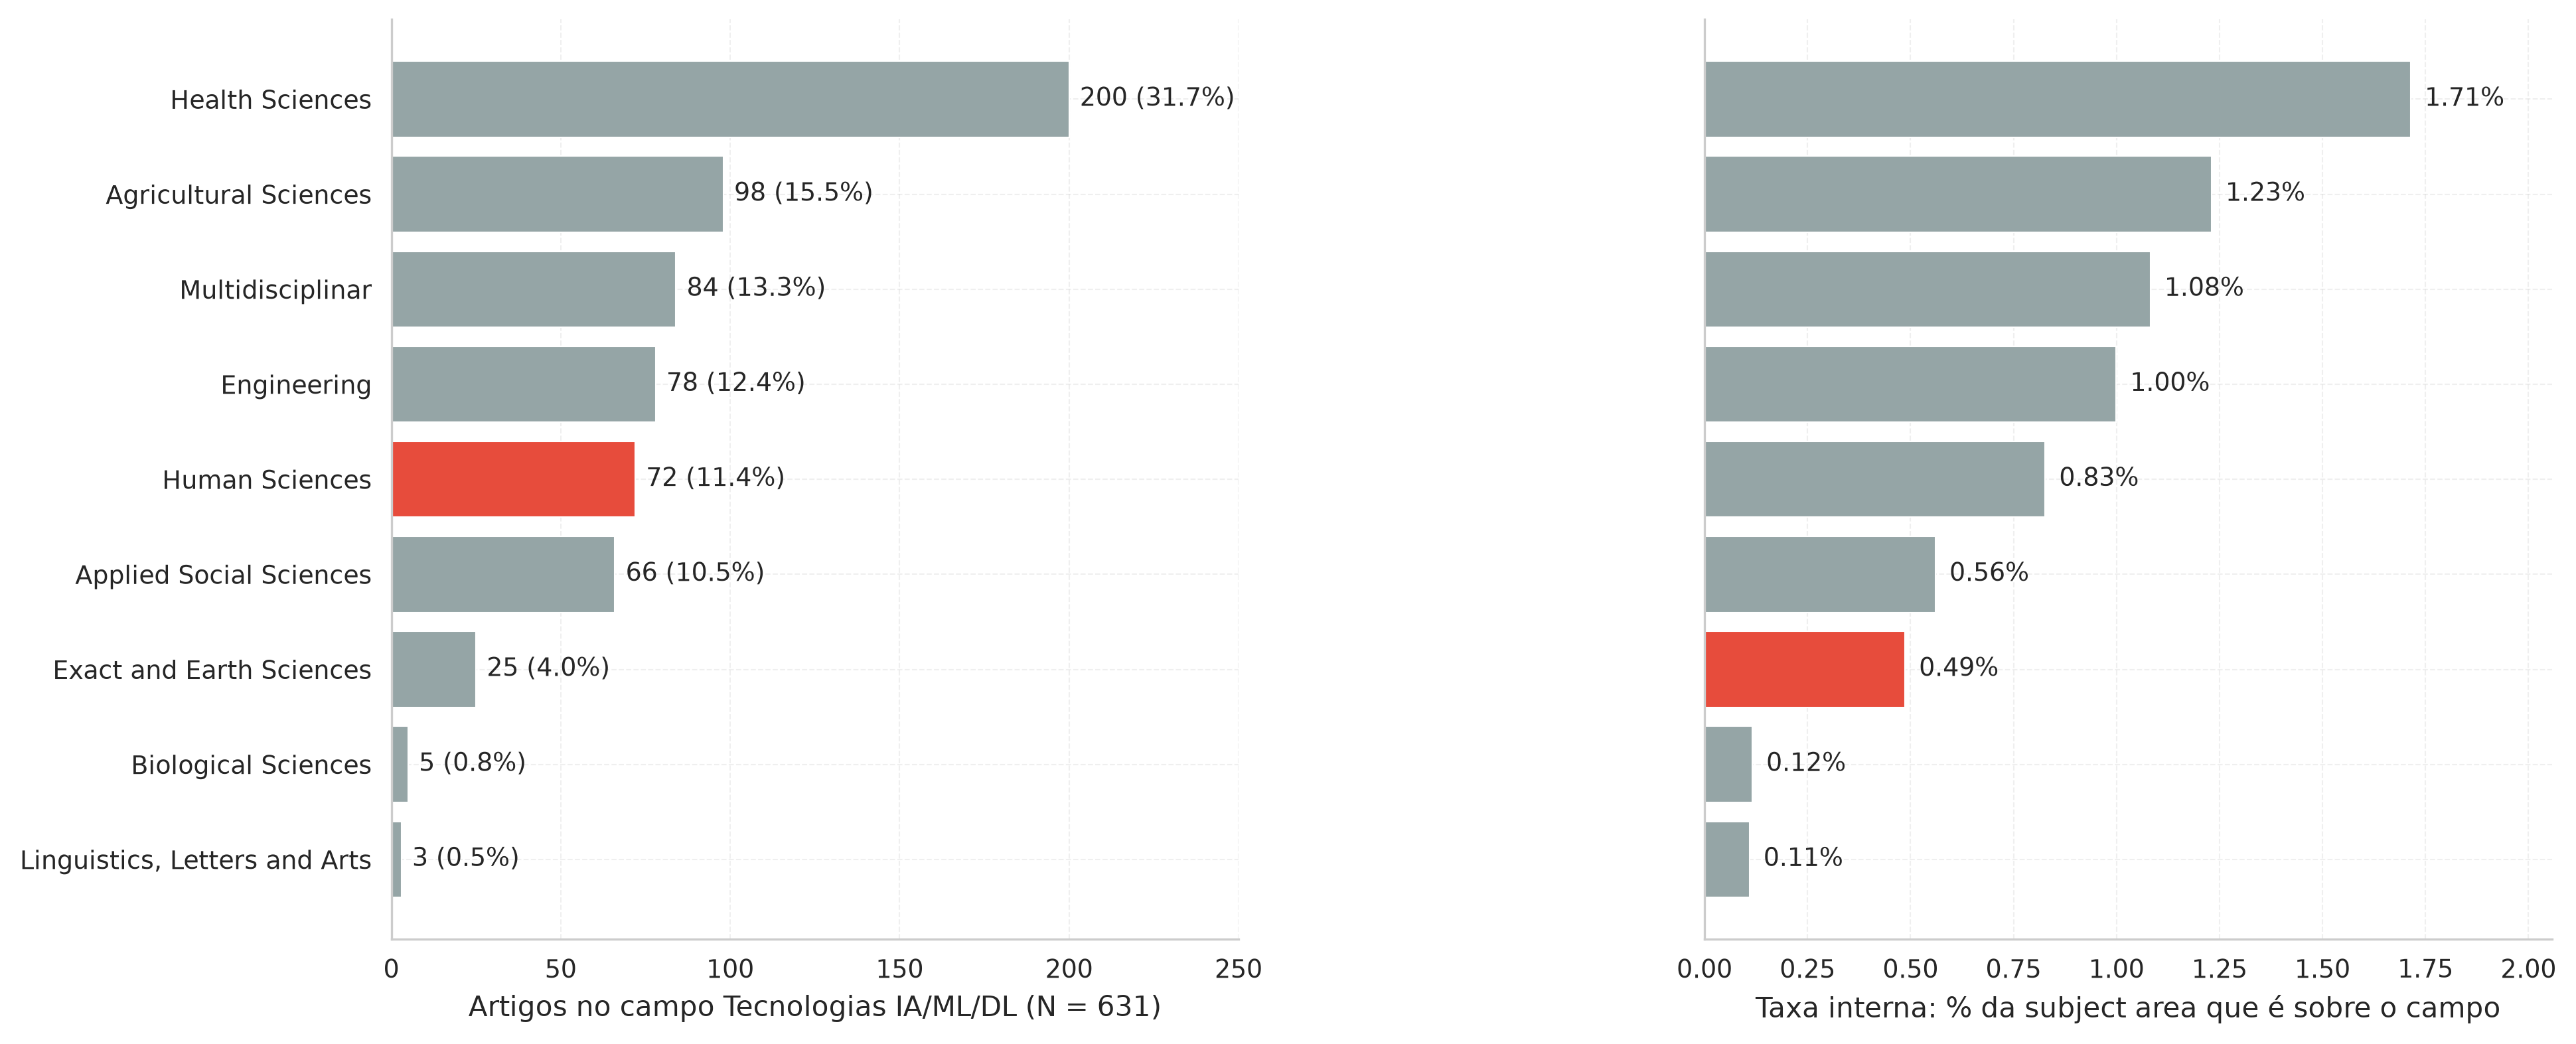
\includegraphics[width=0.95\linewidth]{figuras/cap.2/capes-scielo/scielo_11_subject_area_share.png}
    \caption[Distribuição do corpus \texttt{SciELO} por subject\_area, 2021--2024]{%
        Distribuição dos 631 artigos sobre inteligência artificial, aprendizado de máquina e aprendizado profundo publicados na coleção brasileira do \texttt{SciELO} no quadriênio 2021--2024, pela \emph{subject\_area} primária do periódico. O painel da esquerda mostra o volume absoluto e a participação no corpus, e o painel da direita mostra a taxa interna, isto é, a fração dos artigos de cada área que tocam o campo. As Ciências da Saúde lideram em volume, com 200 artigos, e as Engenharias registram a maior taxa interna, com 1,71\%. As Ciências Humanas, em destaque, respondem por 72 artigos e taxa interna de 0,49\%, magnitude próxima da que a \texttt{Capes} Humanas registra, com 0,67\%. A categoria Multidisciplinar reúne os periódicos cuja classificação no \texttt{SciELO} lista mais de uma área. Elaboração própria a partir da \emph{API} ArticleMeta da coleção brasileira do \texttt{SciELO}. Dados, \emph{scripts} e figuras versionados em \protect\url{https://github.com/julianehelanski/bibliometria-ia-humanas}.}
    \label{fig:scielo_subject_area}
\end{figure}

A interpretação da Figura~\ref{fig:scielo_subject_area} fortalece a primeira camada do achado. As Ciências Humanas, no \texttt{SciELO}, aparecem com 72 artigos e taxa interna de 0,49\%, valor próximo dos 0,67\% que a \texttt{Capes} Humanas registra na produção de pós-graduação. As duas bases foram construídas por plataformas e procedimentos distintos, e descrevem objetos distintos, a tese e o artigo, e ainda assim devolvem a mesma ordem de grandeza para a presença das Ciências Humanas no campo da inteligência artificial. A marginalidade que descrevi pela \texttt{Capes} reaparece quando a base muda da tese e da dissertação para o artigo publicado em periódico, e a convergência entre as duas análises paralelas sustenta a leitura de que essa marginalidade não é efeito do tipo de documento que uma das bases indexa.

Ao distribuir os 631 artigos pelos cinco subcampos do classificador, leio uma segunda diferença entre as duas bases, que disponho na Figura~\ref{fig:scielo_subcampos}. No \texttt{SciELO}, o subcampo mais frequente é a inteligência artificial em sentido estrito, com 187 artigos, ao passo que na \texttt{Capes} esse mesmo subcampo aparece só em quarto lugar, atrás do aprendizado de máquina, que lidera a pós-graduação com 5.284 trabalhos. A hierarquia, em suma, inverte: o que predomina no artigo de periódico é justamente o que rareia na tese. Leio essa inversão como efeito dos dois tipos de escrita que as duas bases capturam, pois o periódico publica a inteligência artificial sobretudo como conceito a discutir, e a pós-graduação a pesquisa sobretudo como técnica a aplicar. Cada veículo privilegia um recorte distinto do campo, e só a leitura das duas bases em paralelo faz com que essa diferença apareça.

\begin{figure}[htbp]
    \centering
    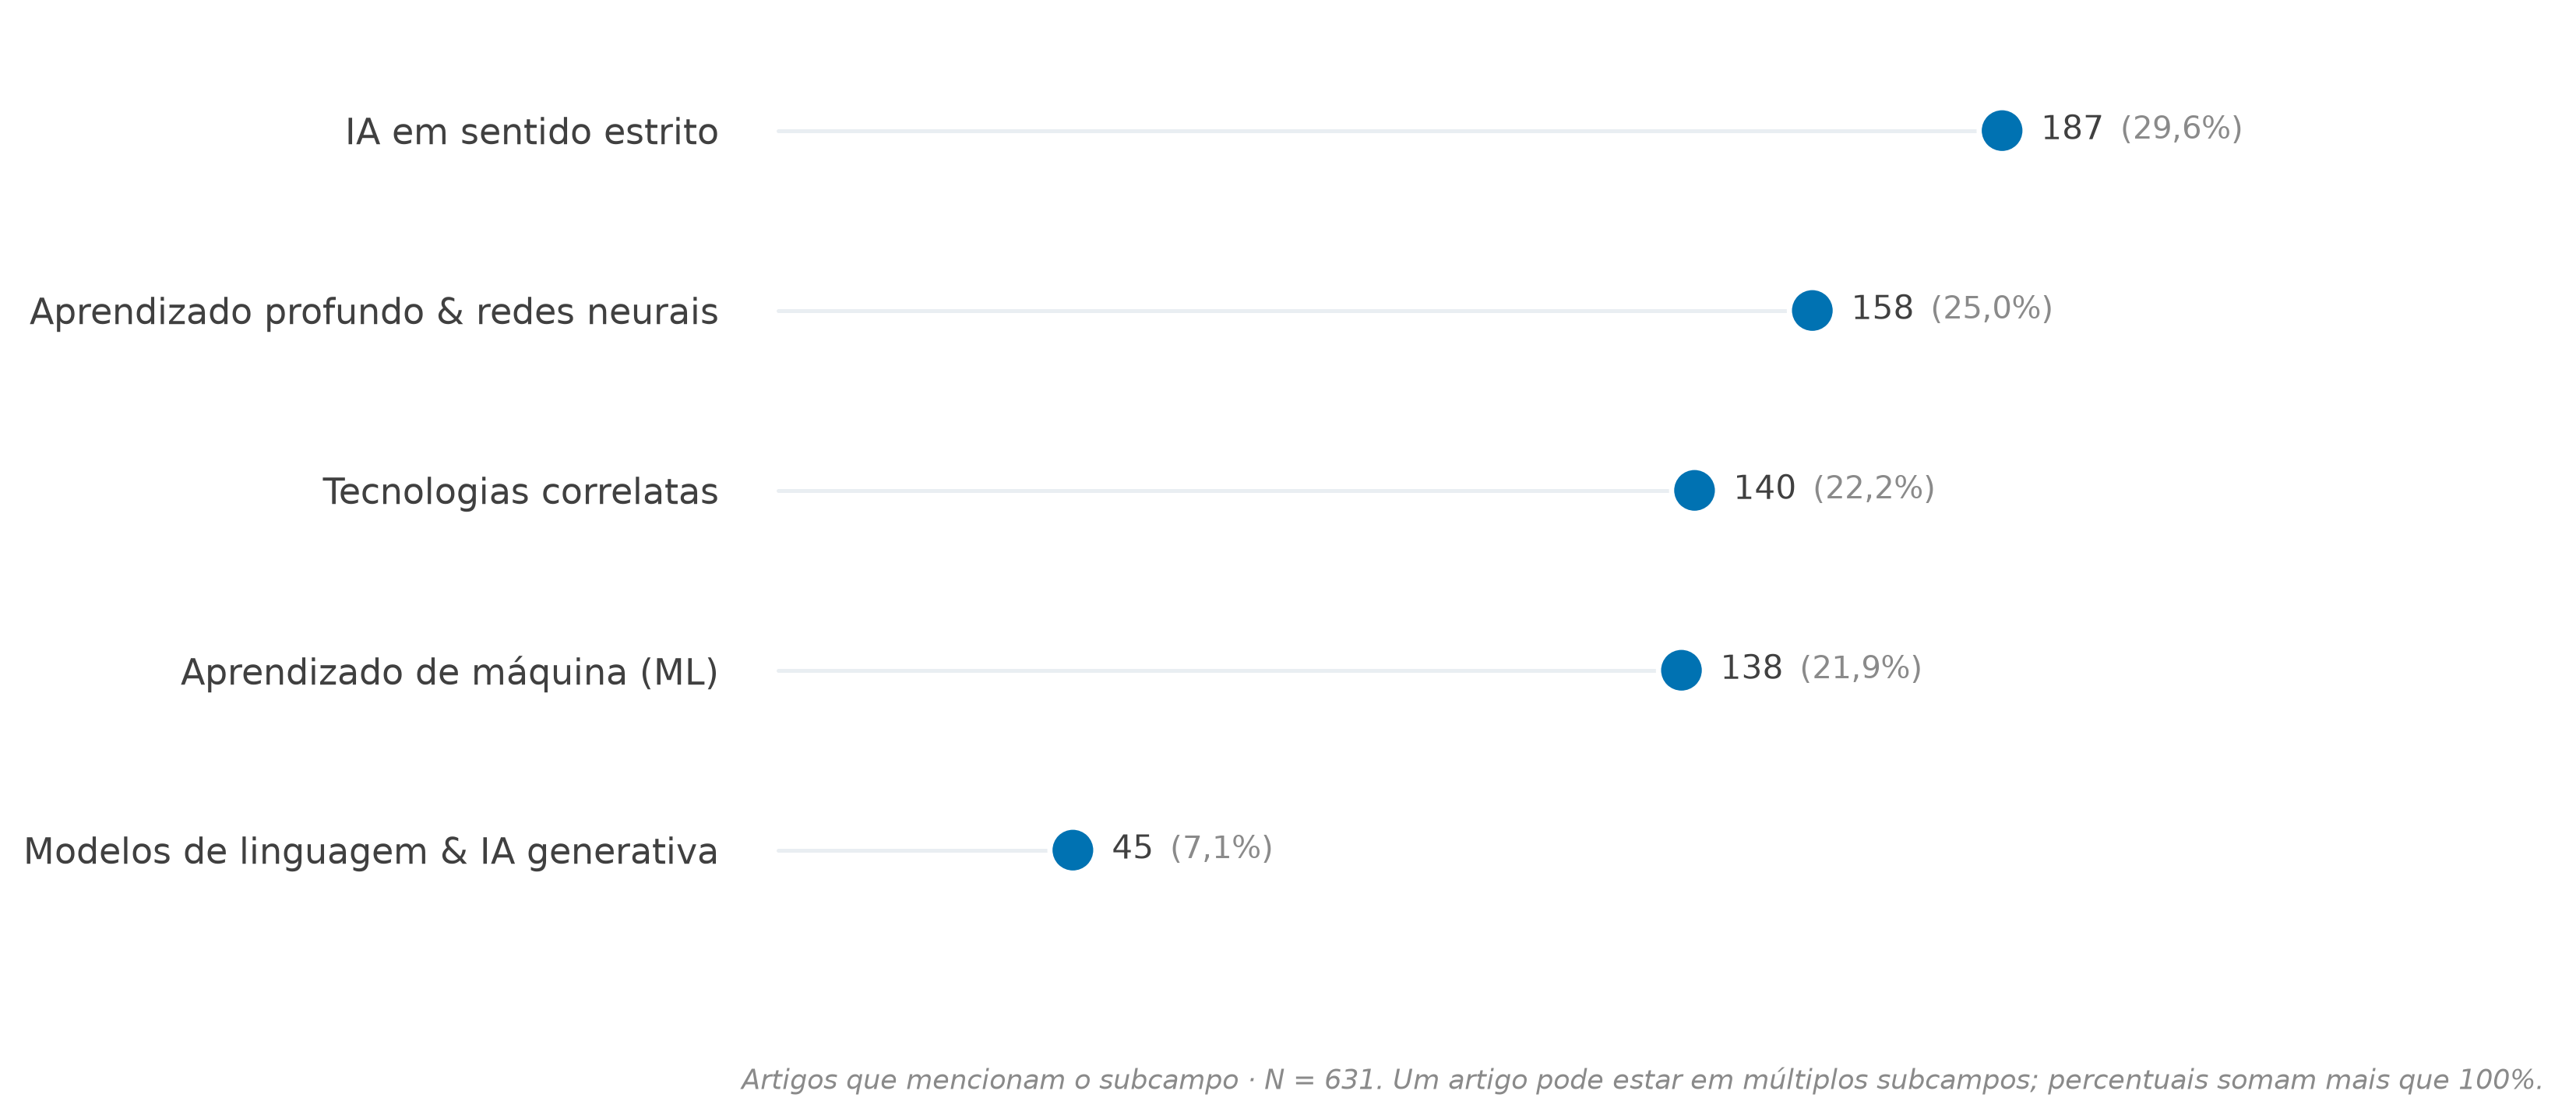
\includegraphics[width=0.85\linewidth]{figuras/cap.2/capes-scielo/scielo_21_subcampos_distribuicao.png}
    \caption[Distribuição do corpus \texttt{SciELO} por subcampo, 2021--2024]{%
        Distribuição dos 631 artigos do corpus \texttt{SciELO} pelos cinco
        subcampos do classificador. Um mesmo artigo pode pertencer a mais de um subcampo, e por isso a soma dos percentuais ultrapassa cem. A inteligência artificial em sentido estrito é o subcampo mais frequente, com 187 artigos, e o aprendizado de máquina aparece em quarto lugar, com 138, atrás das tecnologias correlatas, com 140, hierarquia que inverte a do Catálogo da \texttt{Capes}, em que o aprendizado de máquina lidera. A inversão sustenta a leitura de que o
        periódico publica a inteligência artificial como conceito e a
        pós-graduação a pesquisa como técnica aplicada. Elaboração própria a
        partir da \emph{API} ArticleMeta da coleção brasileira do \texttt{SciELO}. Dados, \emph{scripts} e figuras versionados em \protect\url{https://github.com/julianehelanski/bibliometria-ia-humanas}.}
    \label{fig:scielo_subcampos}
\end{figure}

O \texttt{SciELO} acrescenta um ponto relevante sobre essas publicações, referente aos tipos de veículos que a Antropologia brasileira utiliza para publicar pesquisas sobre inteligência artificial.\footnote{O recorte de Ciências Humanas que comparo com a \texttt{Capes} é o subset das Ciências Humanas em sentido estrito, isto é, os 72 artigos publicados em periódicos cuja \emph{subject\_area} é exatamente \enquote{Human Sciences}, sem a categoria Multidisciplinar. Esse recorte estrito é o que estabelece a paridade com a grande área Ciências Humanas do Catálogo da \texttt{Capes}, e dele que saem os números de periódicos discutidos neste parágrafo.} No subset das Ciências Humanas em sentido estrito, a revista \textit{Mana}, periódico de referência da Antropologia brasileira, aparece com três artigos. Os três foram publicados em 2024, e os três tocam o campo pela porta do \emph{big data}, e não da inteligência artificial em sentido estrito. A Antropologia, quando entra na conversa em seu próprio periódico de referência, entra tarde, em 2024, e por um vocabulário deslocado em relação ao objeto. O achado do \texttt{SciELO} compõe com o da \texttt{Capes} uma leitura em duas camadas: a \texttt{Capes} mostra a escassez da tese e da dissertação de Antropologia sobre inteligência artificial, e o \texttt{SciELO} mostra que, quando a disciplina publica o artigo, publica-o pelo tema \emph{big data}. As duas bases, cada uma com seu objeto, sustentam o mesmo diagnóstico de uma emergência tardia e tematicamente deslocada.

O mapeamento que fiz nesta seção mostra que as duas bases estão alinhadas em seus principais achados. O primeiro é que o acesso ampliado à inteligência artificial generativa, a partir do final de 2022, produziu uma aceleração visível nas duas ao mesmo tempo, na produção de pós-graduação que a \texttt{Capes} reúne e na produção de periódico que a \texttt{SciELO} reúne. O segundo é que a presença da inteligência artificial nas ciências humanas, além de pequena, distribui-se de modo desigual por dentro. As duas bases chegam à mesma ordem de grandeza para o conjunto das Ciências Humanas por caminhos separados, 0,67\% das defesas na \texttt{Capes} e 0,49\% dos artigos na \texttt{SciELO}, duas medidas próximas obtidas sobre objetos distintos, a tese e o artigo, e a proximidade entre elas me autoriza a ler esses números como característica do próprio campo, e não como efeito do documento que cada base indexa. Dentro desse conjunto já reduzido, a distribuição é ainda maior: a Educação concentra 38,5\% das defesas, ao passo que a Antropologia, com quatro defesas e 1,0\%, aparece quase no fim, à frente apenas da Arqueologia.

A dispersão temática que encontro nas duas bases, da automação industrial à arte contemporânea, do policiamento preditivo às estatísticas oficiais, da saúde da mulher ao \emph{big data} eleitoral, suscita algumas questões que deixo em aberto. Será que o campo está disperso porque o objeto é, ele próprio, heterogêneo? A inteligência artificial abrange várias técnicas, infraestruturas e relações que se ramificam por toda parte. Pode ser que esteja disperso porque as ciências humanas brasileiras são plurais por constituição, e cada disciplina encontra a inteligência artificial pela vizinhança dos seus próprios objetos. Pode ser, ainda, que o campo seja novo demais para ter convergido, e que a dispersão de hoje seja a forma provisória de um campo em formação. Ou pode ser que essa dispersão não seja transitória nem acidental, e sim o indício de algo mais estrutural, a saber, que a inteligência artificial já está tão entranhada no trabalho, na política, na saúde e na cultura que pesquisá-la em separado, como objeto autônomo, talvez seja a abordagem menos provável justamente porque ela está em toda parte. Inclino-me para essa última leitura, sem descartar as outras, e deixo a tensão entre elas como uma das perguntas que estudos futuros poderão investigar com mais profundidade.

A Figura~\ref{fig:comparativo_scielo_capes} reúne essa leitura paralela das duas bases brasileiras em quatro painéis, com o mesmo classificador de cinco subcampos aplicado às duas e com recorte de escopo equivalente, a \texttt{SciELO} restrita ao subset de Ciências Humanas em sentido estrito e a \texttt{Capes} restrita à grande área Ciências Humanas. Os dois painéis superiores cruzam a evolução temporal e a distribuição por subcampo, e as duas bases crescem em ritmo próximo, 112\% na \texttt{SciELO} e 106\% na \texttt{Capes} entre 2021 e 2024, e cada uma pende para um lado, o periódico para a inteligência artificial como conceito e a tese para a técnica aplicada. Os dois painéis inferiores descem ao detalhe de cada base, os periódicos de Ciências Humanas em que a \texttt{SciELO} concentra os artigos e as áreas de conhecimento em que a \texttt{Capes} concentra as defesas, e situam, nos dois recortes, a posição marginal da Antropologia: cada base alcança um aspecto que a outra não vê, pois a \texttt{Capes} reúne programas e dá a leitura caso a caso das quatro defesas, e o \texttt{SciELO} reúne periódicos e dá os três artigos da revista \textit{Mana}, e os dois recortes fecham a mesma figura de uma disciplina que entra no campo por último e por uma porta lateral.

\begin{figure}[htbp]
    \centering
    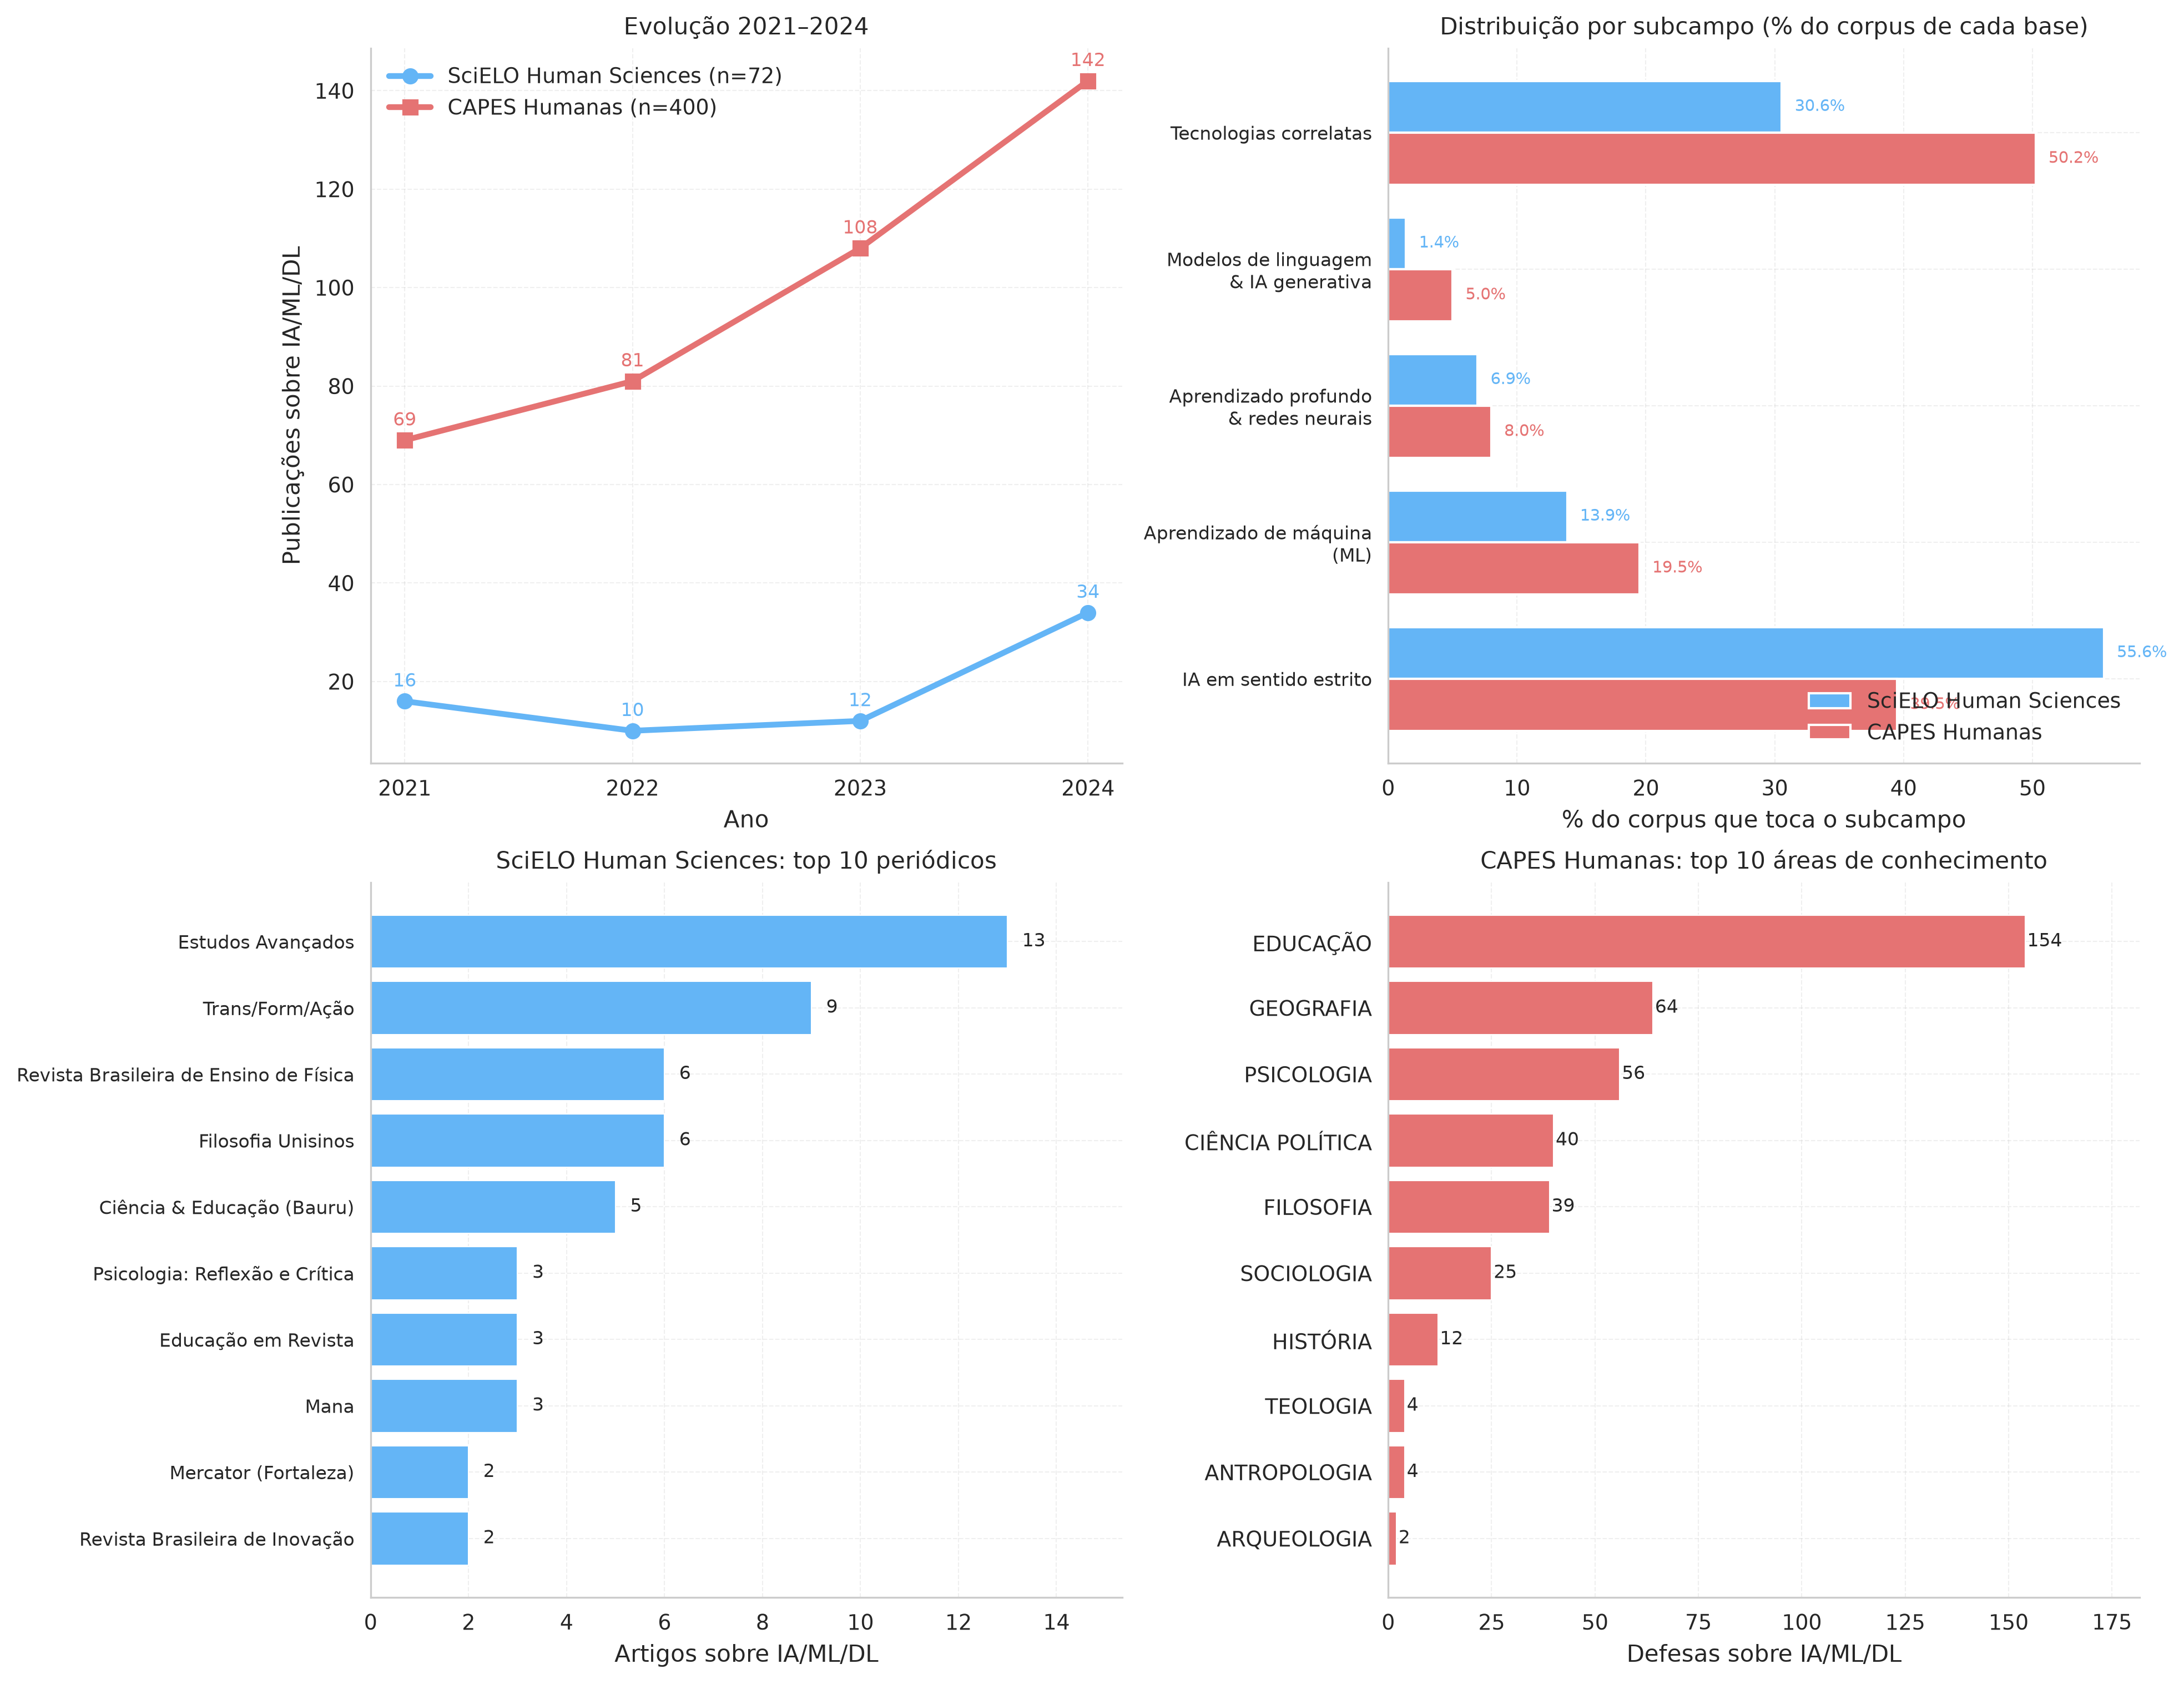
\includegraphics[width=1.0\linewidth]{figuras/cap.2/capes-scielo/comparativo_scielo_capes_2026.png}
    \caption[Análise comparativa \texttt{SciELO} e \texttt{Capes} nas Ciências Humanas, 2021--2024]{%
        Leitura paralela das duas bases sobre o quadriênio 2021--2024, com o
        mesmo classificador de cinco subcampos aplicado a cada uma e recorte de
        escopo equivalente: o \texttt{SciELO} restrito ao subset de Ciências
        Humanas em sentido estrito, sem a categoria Multidisciplinar, e a
        \texttt{Capes} restrita à grande área Ciências Humanas. O painel A
        sobrepõe a evolução temporal: o \texttt{SciELO} de Ciências Humanas
        cresce de 16 para 34 artigos sobre o campo, e a \texttt{Capes} Humanas
        cresce de 69 para 142 defesas. O painel B põe lado a lado a distribuição
        por subcampo, com o \texttt{SciELO} mais inclinado à inteligência
        artificial como conceito e a \texttt{Capes} mais inclinada às
        tecnologias correlatas, sobretudo pelo caminho da Educação. O painel C traz
        os dez periódicos do \texttt{SciELO} de Ciências Humanas com mais
        artigos no campo, com \textit{Estudos Avançados} à frente, com 13, e a
        revista de Antropologia \textit{Mana} com 3. O painel D traz as dez
        áreas de conhecimento das defesas da \texttt{Capes} Humanas, com a
        Educação à frente, com 154, e a Antropologia com 4. Elaboração própria
        a partir da \emph{API} ArticleMeta da coleção brasileira do
        \texttt{SciELO} e do Catálogo de Teses e Dissertações da \texttt{Capes},
        \emph{dump} oficial \texttt{BR-CAPES-BTD-2021A2024}. Dados, \emph{scripts} e figuras versionados em \protect\url{https://github.com/julianehelanski/bibliometria-ia-humanas}.}
    \label{fig:comparativo_scielo_capes}
\end{figure}

A posição da antropologia dentro das ciências humanas se inscreve, por sua vez, na posição do Brasil no mapa mundial da inteligência artificial, como uma \enquote{semiperiferia} em movimento. Pelo levantamento do \texttt{CSET} (\emph{Center for Security and Emerging Technology}), que reúne artigos, trabalhos de conferência e \emph{preprints} sobre inteligência artificial em todas as áreas do conhecimento, o Brasil ocupou em 2024 a vigésima terceira posição mundial, com pouco mais de três mil publicações, e liderou com folga a América Latina \parencite{OWID2024AI}. Esta não é uma posição de quem está fora do mapa. O que me chama a atenção é o movimento da produção brasileira, que cresceu em números absolutos ao longo da década, e ainda assim recuou da décima terceira posição que ocupava em 2016 para a vigésima terceira em 2024, porque a aceleração de outros países foi mais rápida que a sua. O mesmo movimento aparece no mapeamento dos centros de inteligência artificial da \texttt{FAPESP}, que registra um Brasil entre os vinte maiores produtores em volume e, ao mesmo tempo, distante da fronteira de ponta, com presença discreta nas conferências de referência e produção concentrada em poucas instituições, com a \texttt{USP} à frente \parencite{Brandao2024Desenvolvimento}. É essa concentração que a própria política de criação dos centros, entre eles o \texttt{C4AI} de que trato no capítulo~\ref{capitulo3}, procura corrigir. As ciências humanas e sociais se aproximam da inteligência artificial a partir desse contexto geral de produção tecnocientífica de peso intermediário em escala mundial, de grande relevância na região e em relativo recuo, longe da periferia e longe do atraso.

O levantamento do \texttt{CSET} mede a inteligência artificial sem recorte de disciplina, e por isso não me diz onde, dentro da produção de cada país, a inteligência artificial entra. Para descer ao recorte que interessa à minha pesquisa, a inteligência artificial dentro das ciências humanas, recorri a uma terceira base, o \texttt{OpenAlex}, catálogo aberto de cerca de duzentos e cinquenta milhões de obras acadêmicas de todo o mundo.\footnote{O \texttt{OpenAlex} é um catálogo bibliográfico aberto, mantido pela organização \texttt{OurResearch} desde 2022 como sucessor do \texttt{Microsoft Academic Graph}, e indexa obras, autorias, instituições e os conceitos a elas atribuídos por classificação automática. Coletei o corpus com o \texttt{claude code} no terminal, em sessões iteradas de requisição à \emph{API} \emph{REST} da plataforma, classificação e auditoria, e apliquei a ele a mesma régua de cinco subcampos que apliquei ao Catálogo da \texttt{Capes} e à \texttt{SciELO}, de modo que os subcampos ficam comparáveis entre as três bases. Os números canônicos do recorte do \texttt{OpenAlex}, e a proveniência de cada figura, ficam versionados no arquivo \texttt{docs/decisoes\_metodologicas.md} do repositório.} O que faltava à \texttt{Capes} e à \texttt{SciELO}, e que o \texttt{OpenAlex} me dá, é a comparação por país e por disciplina ao mesmo tempo, isto é, a possibilidade de cruzar o conceito de inteligência artificial com a classificação das obras por \emph{field}, o campo do conhecimento que a taxonomia da plataforma herda da base \texttt{Scopus}.\footnote{O \emph{field} é a unidade intermediária da taxonomia do \texttt{OpenAlex}, importada da classificação \emph{ASJC} (\emph{All Science Journal Classification}) da \texttt{Scopus}, comunidade da bibliometria internacional. Para espelhar a grande área Ciências Humanas do Catálogo da \texttt{Capes}, que abriga também a Psicologia, adotei o recorte amplo que reúne três \emph{fields}, o de Artes e Humanidades, o de Psicologia e o de Ciências Sociais. A escolha do recorte é uma decisão metodológica, e não um dado, e por isso a declaro: outra pesquisadora que adotasse só o \emph{field} de Artes e Humanidades, ou que somasse outros \emph{fields}, encontraria magnitudes distintas. Os identificadores dos três \emph{fields} foram conferidos diretamente na \emph{API} em seu estado de seis de junho de 2026, porque a taxonomia da plataforma evolui no tempo. A janela é 2016--2024, alinhada à do \texttt{CSET}.}

Antes de partir aos números do \texttt{OpenAlex}, preciso enfrentar uma divergência que a base devolve sobre si mesma, e que toca o problema que percorre esta seção inteira, o de saber o que conta como inteligência artificial. A mesma base, sobre o mesmo recorte brasileiro de humanidades, produz dois números muito distantes conforme o critério que escolho para dizer que uma obra é de inteligência artificial. Pelo conceito que o próprio \texttt{OpenAlex} atribui às obras por classificação automática, o Brasil registra 9.996 obras de inteligência artificial nas humanidades no período; pela régua de palavra-chave, a mesma que sustenta os números da \texttt{Capes} e da \texttt{SciELO}, apenas 849 obras únicas trazem, de fato, vocabulário de inteligência artificial no título ou no resumo. Somente cerca de 8,5\% das obras que o classificador do \texttt{OpenAlex} marca como inteligência artificial contêm esse vocabulário explícito, e leio esse abismo de duas maneiras que se somam: o conceito atribuído pela máquina é generoso e alcança obras que apenas tangenciam o campo, e parte das obras indexadas não traz resumo, o que deixa a régua de palavra-chave com menos texto para cruzar.\footnote{O conceito \enquote{\emph{Artificial intelligence}} do \texttt{OpenAlex} é atribuído por um modelo de classificação que lê os metadados de cada obra e lhe associa conceitos com um grau de confiança, e por isso alcança obras cuja relação com o campo é de vizinhança temática, e não de objeto. A régua de palavra-chave, ao contrário, exige a presença de um termo do campo no título ou no resumo, e é, das duas, a mais próxima do gesto que faço nas outras bases. O número comparável à \texttt{Capes} e à \texttt{SciELO} é o das 849 obras únicas, e não o das 9.996. A contagem por obra única deduplica a contagem por afiliação, em que uma obra é somada uma vez para cada país de seus autores, e que para o Brasil chegava a 15.438 registros, inflada pela coautoria internacional.} Esse desencontro entre os dois critérios me mostra que medir a presença da inteligência artificial exige, antes de tudo, uma decisão sobre o que se está disposto a chamar de inteligência artificial, e a distância entre 9.996 e 849 é a distância entre um campo tomado por vizinhança conceitual e um campo tomado por nomeação explícita. Por isso a comparação internacional de volume e de penetração, mais uniforme entre países, segue o conceito da plataforma, e a análise de subcampos, que precisa falar a mesma língua das outras duas bases, segue a régua de palavra-chave.

\begin{figure}[htbp]
    \centering
    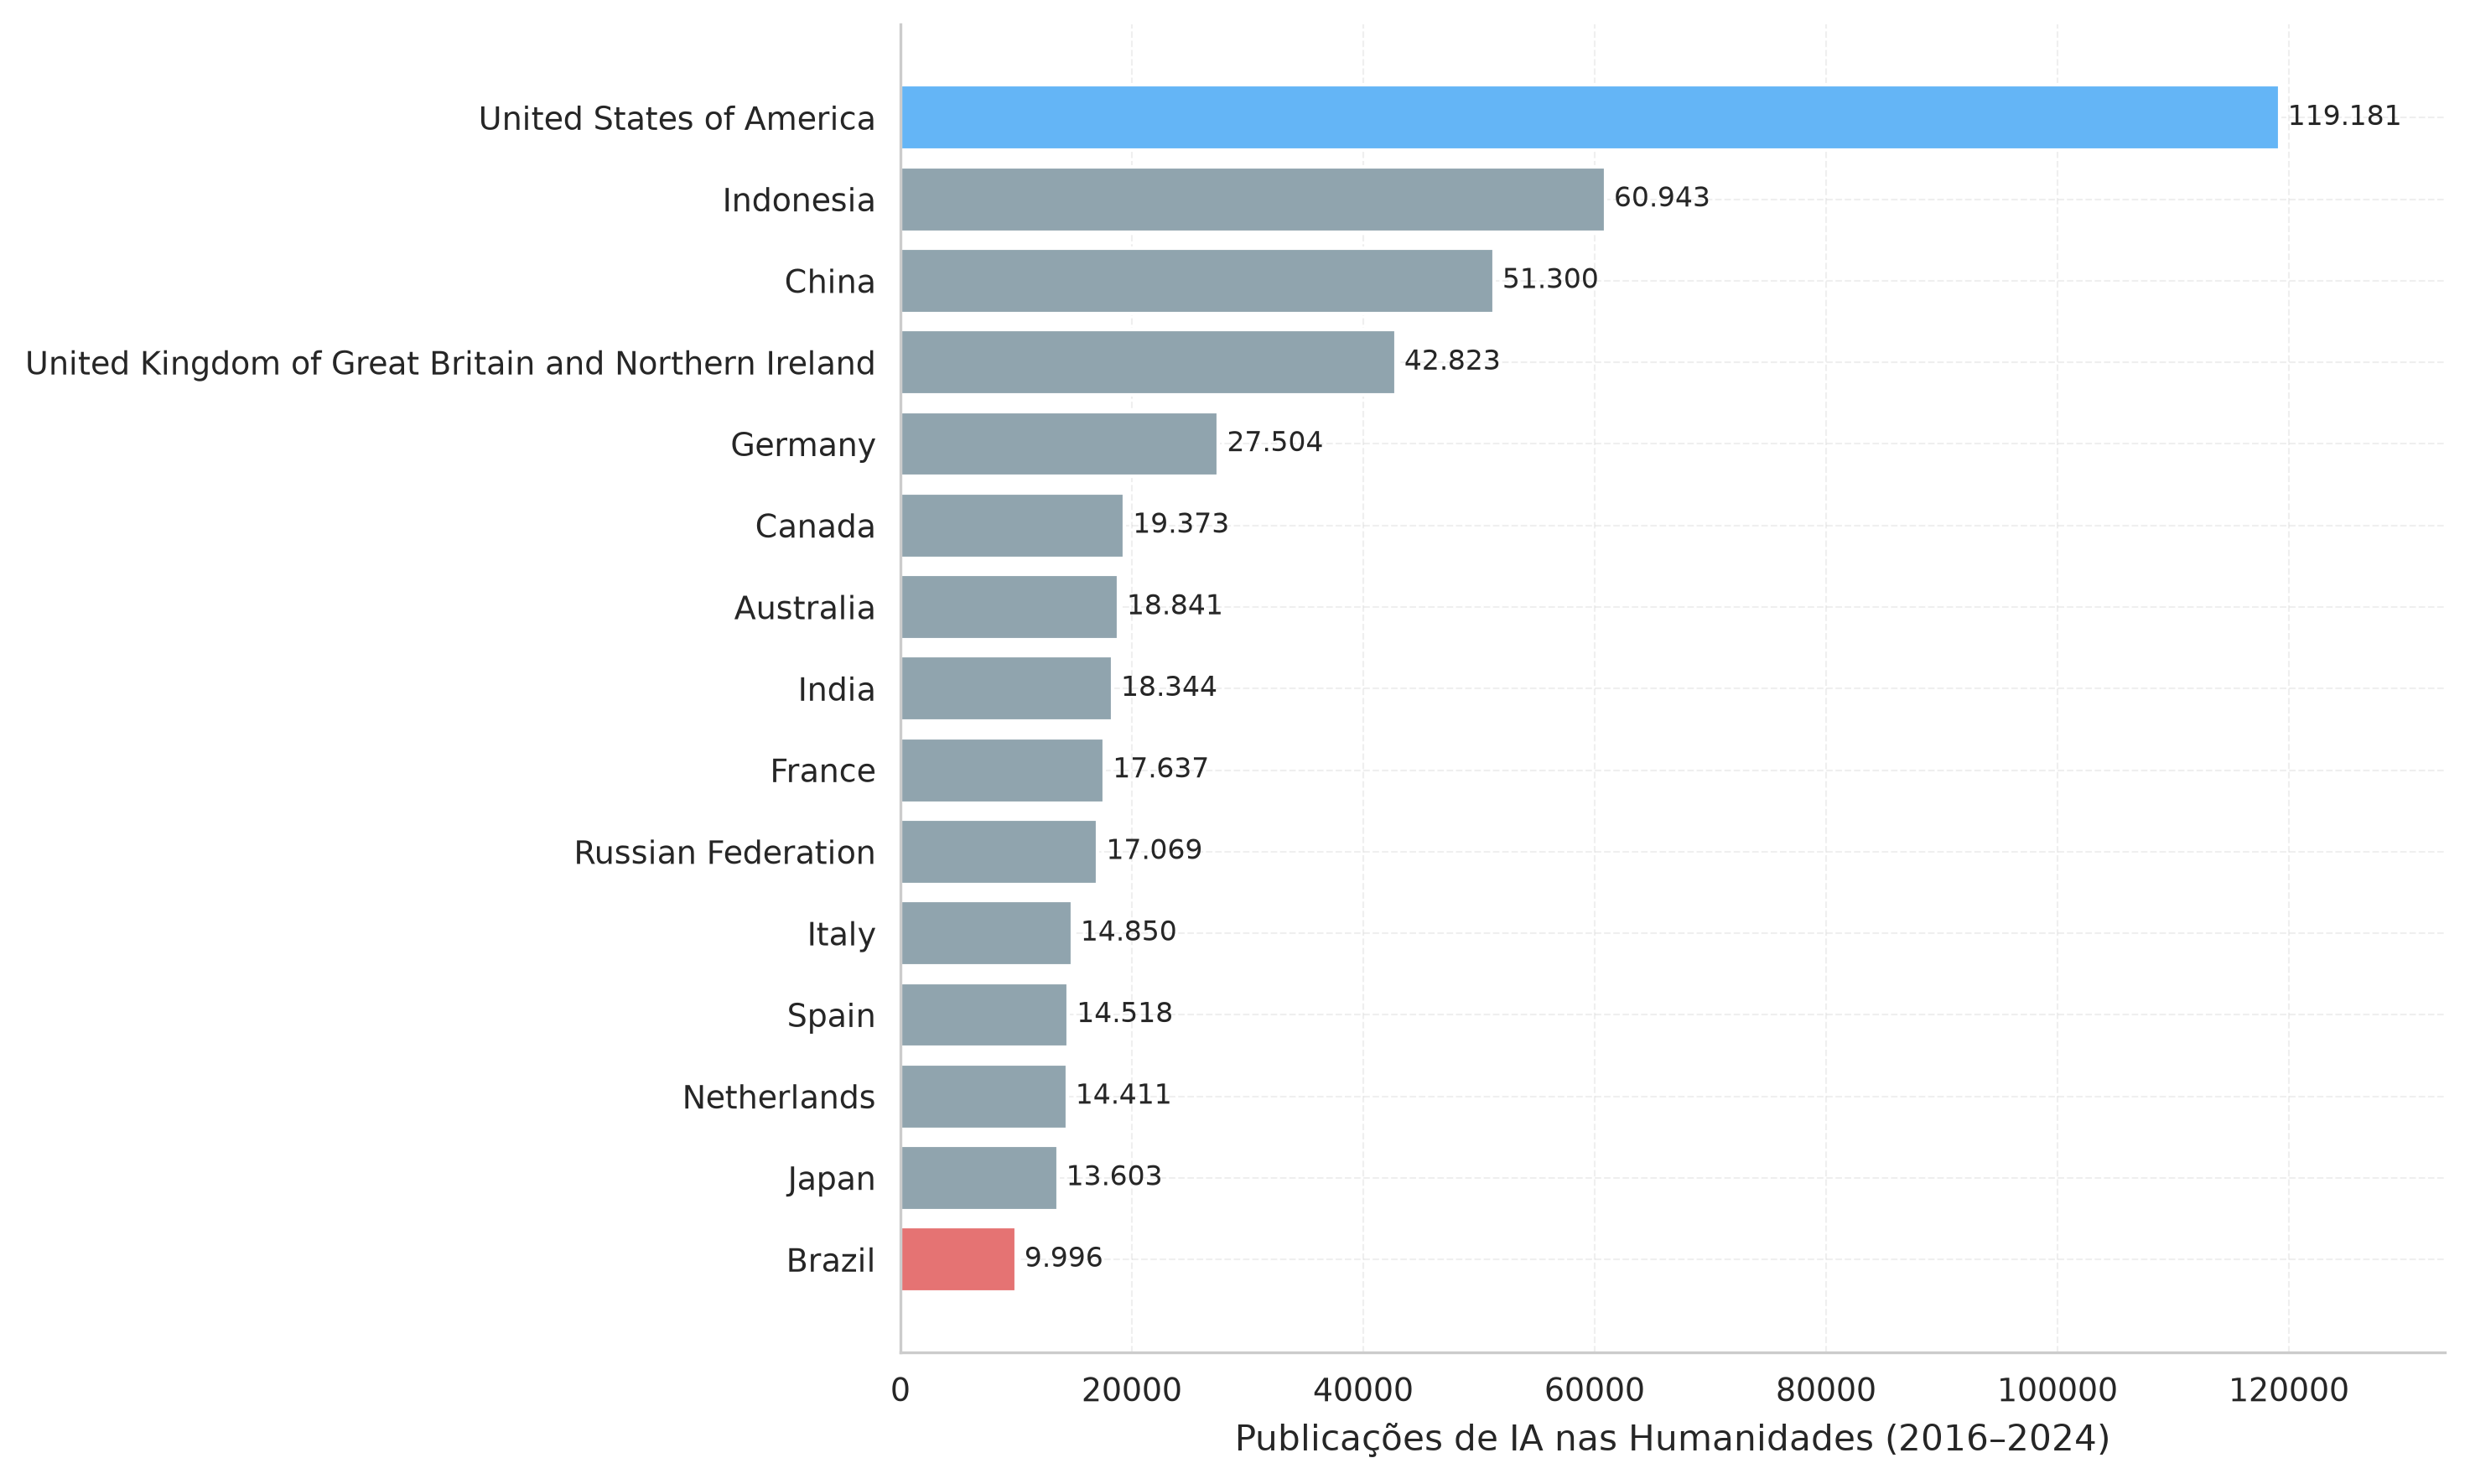
\includegraphics[width=0.85\linewidth]{figuras/cap.2/openalex_01_ranking_paises.png}
    \caption[Maiores produtores de IA nas Humanidades, \texttt{OpenAlex} 2016--2024]{%
        Os quinze maiores produtores de obras sobre inteligência artificial na
        grande área de Humanidades no período 2016--2024, pela definição por
        conceito do \texttt{OpenAlex}, em volume absoluto. O Brasil, em destaque,
        ocupa a décima quinta posição mundial, com 9.996 obras, atrás de
        produtores como os Estados Unidos, com cerca de 119 mil, a China, com
        51,3 mil, o Reino Unido, com 42,8 mil, e a Alemanha, com 27,5 mil. A
        Indonésia, em segundo lugar, e a Índia, em oitavo, sobem no volume
        porque têm universos de humanidades muito grandes, e essa presença
        antecipa por que a leitura por volume precisa ser corrigida pela taxa
        interna. Elaboração própria a partir do \texttt{OpenAlex}. Repositório
        com dados, \emph{scripts} e figuras em \protect\url{https://github.com/julianehelanski/bibliometria-ia-humanas}.}
    \label{fig:openalex_ranking_paises}
\end{figure}

A Figura~\ref{fig:openalex_ranking_paises} mostra uma concentração geográfica acentuada, com os Estados Unidos e a China à frente por larga distância, seguidos do Reino Unido e da Alemanha. Uma inversão me interessa de perto: nas estatísticas de inteligência artificial em todas as áreas, como as do \texttt{CSET} que citei acima, a China supera os Estados Unidos em volume, e quando o recorte se fecha sobre as humanidades os Estados Unidos retomam a dianteira. A interseção entre inteligência artificial e humanidades tem geografia própria, distinta da inteligência artificial tomada em sentido amplo, e por isso o ranking do \texttt{OpenAlex} que leio aqui não é o mesmo que o do \texttt{CSET} do parágrafo anterior, pois um mede o campo inteiro e o outro mede o recorte disciplinar. O Brasil, com 9.996 obras, figura em décimo quinto lugar, presença que não é desprezível em volume absoluto, e que, vista assim, repete a leitura de semiperiferia que o \texttt{CSET} já dava. O volume, porém, esconde o achado, e é a próxima figura que o revela.

\begin{figure}[htbp]
    \centering
    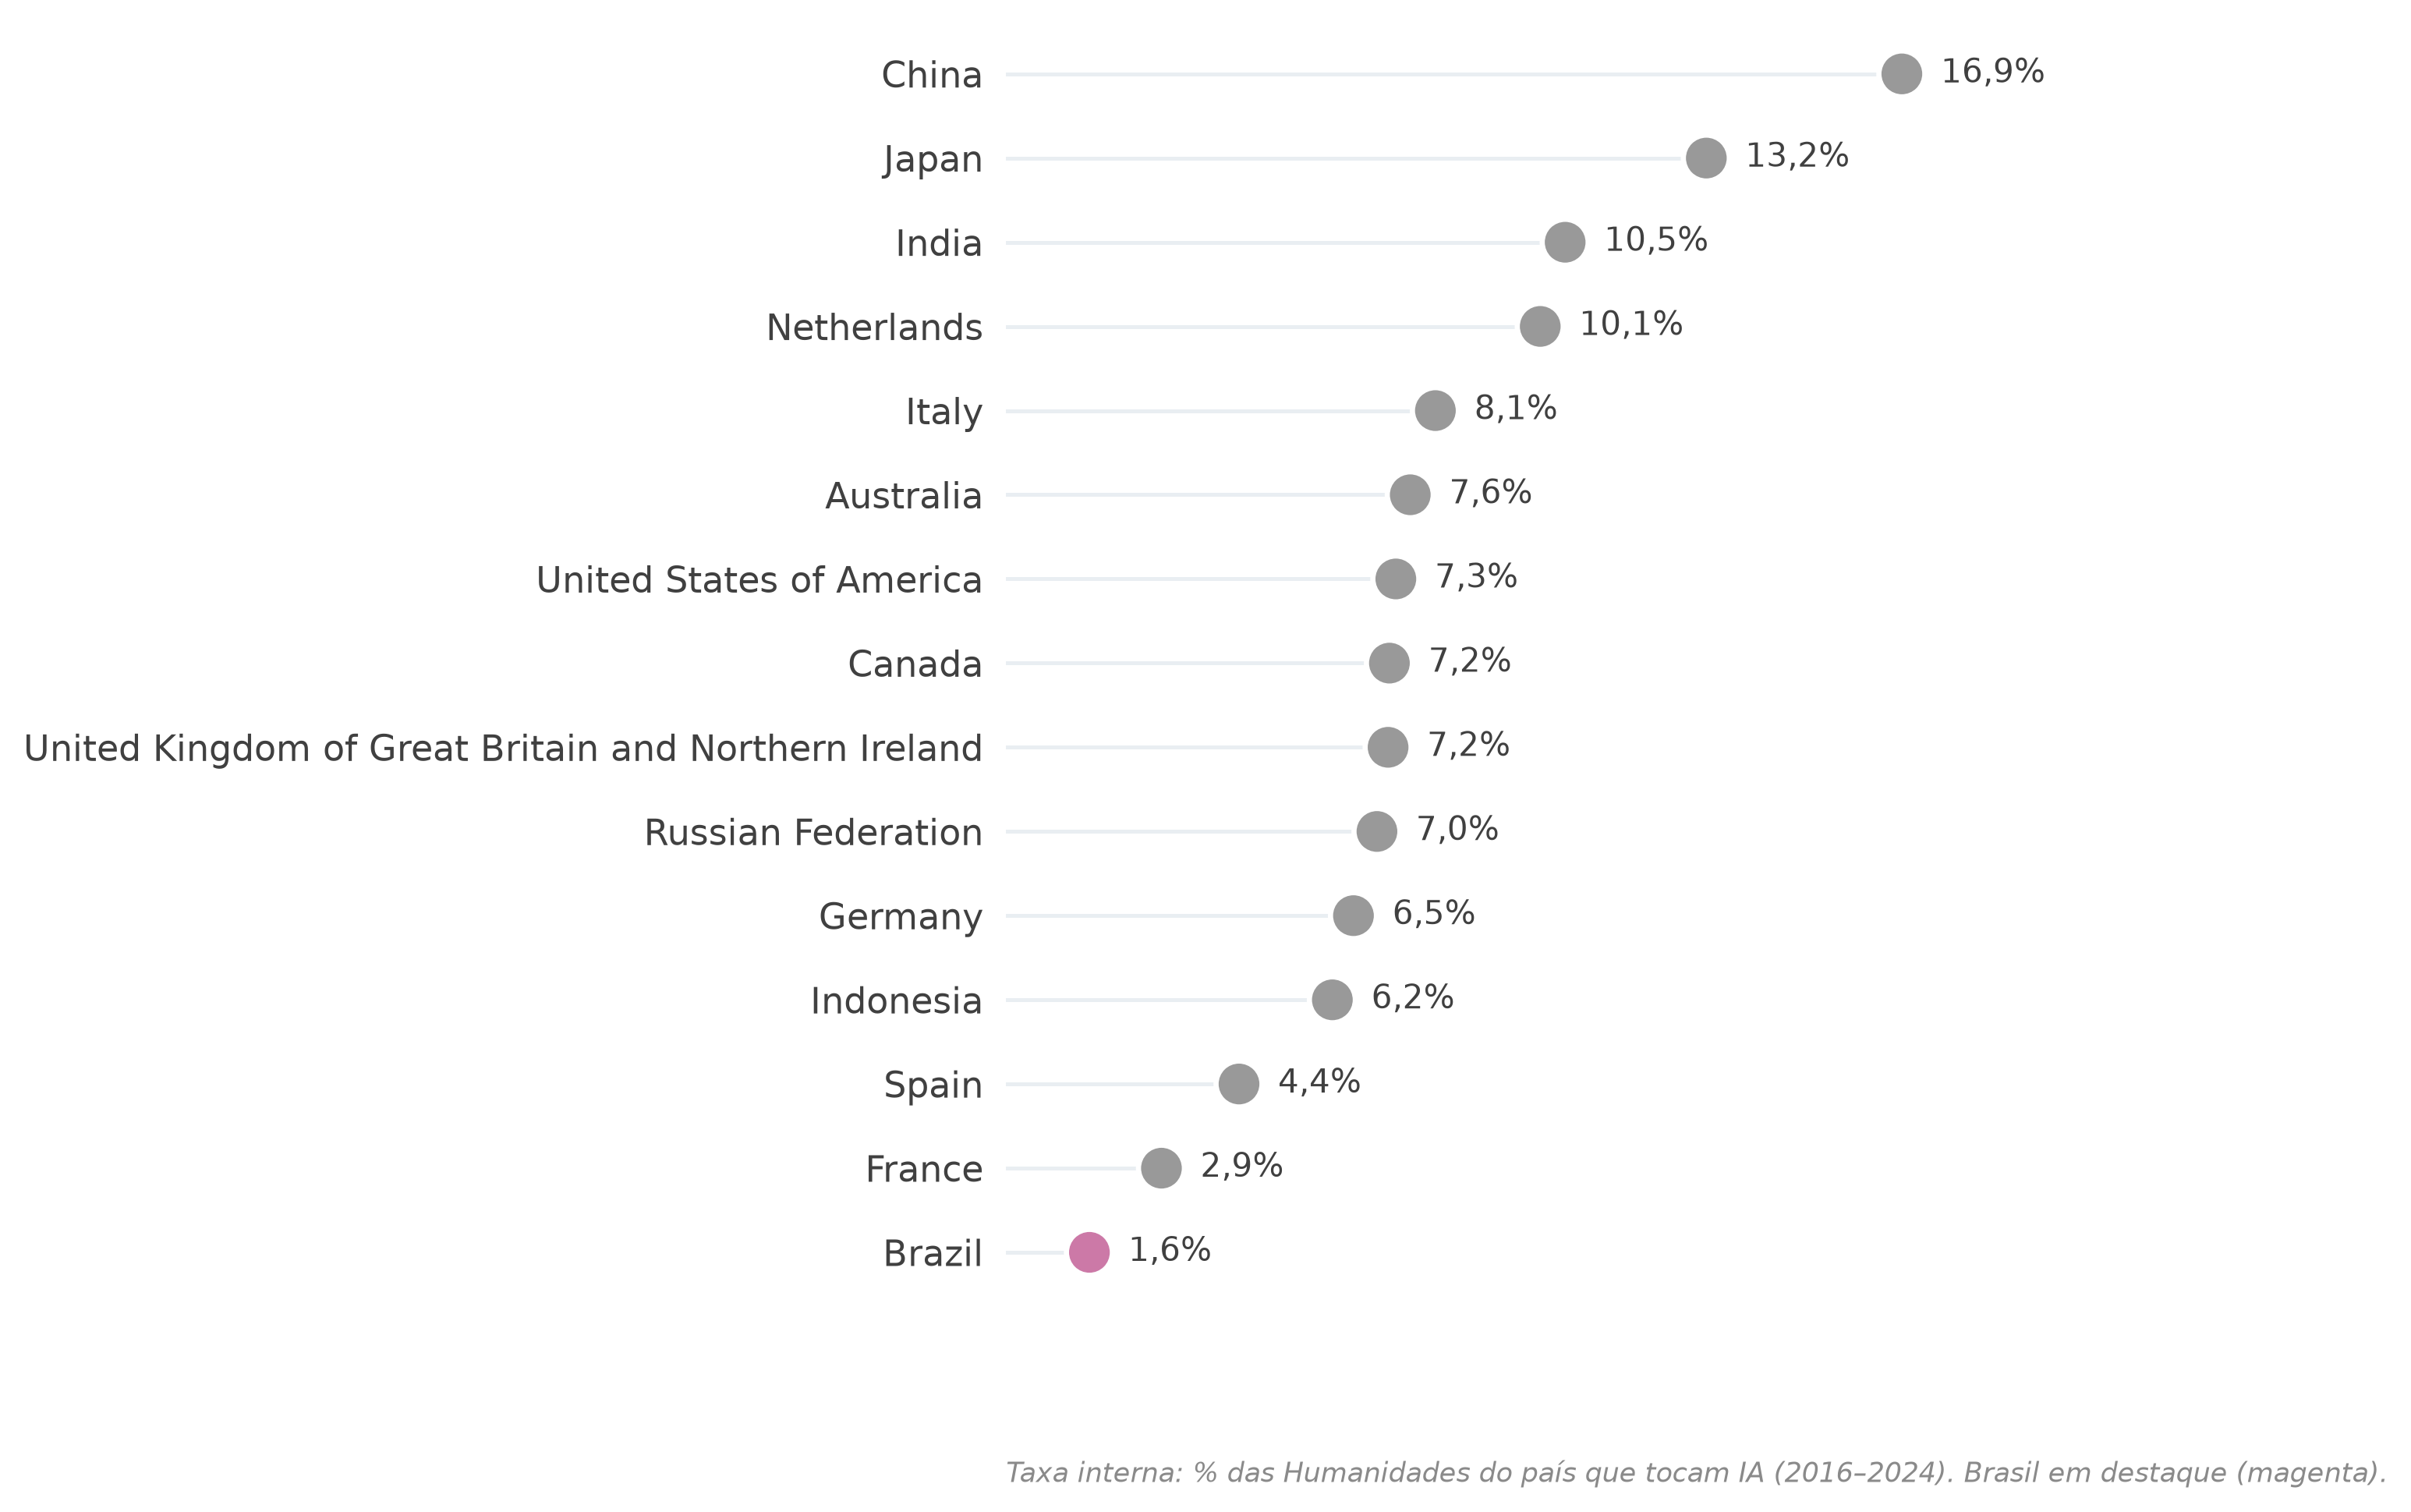
\includegraphics[width=0.85\linewidth]{figuras/cap.2/openalex_02_taxa_interna_paises.png}
    \caption[Taxa interna de IA nas Humanidades por país, \texttt{OpenAlex} 2016--2024]{%
        Taxa interna, isto é, a fração das obras de Humanidades de cada país que
        tocam o campo da inteligência artificial, entre os quinze maiores
        produtores em volume, no período 2016--2024, pela definição por
        conceito do \texttt{OpenAlex}. Apesar do volume que o coloca em décimo
        quinto lugar, o Brasil, em destaque, apresenta a menor taxa do grupo,
        com 1,57\%, contra 16,89\% da China, 13,20\% do Japão e 6,15\% dos
        Estados Unidos. O Brasil tem o segundo maior universo de Humanidades do
        conjunto, com 636.607 obras, atrás apenas dos Estados Unidos, e ainda
        assim é o que menos conecta essa produção à inteligência artificial.
        Elaboração própria a partir do \texttt{OpenAlex}. Repositório com dados,
        \emph{scripts} e figuras em \protect\url{https://github.com/julianehelanski/bibliometria-ia-humanas}.}
    \label{fig:openalex_taxa_interna}
\end{figure}

A leitura por taxa interna, a fração das humanidades de cada país que dialoga com a inteligência artificial, inverte o quadro que o volume sugere, e a Figura~\ref{fig:openalex_taxa_interna} a apresenta. A China lidera a penetração, com 16,89\%, seguida do Japão, com 13,20\%, da Índia, com 10,54\%, e dos Países Baixos, com 10,07\%, e os Estados Unidos, primeiros em volume, ficam em um patamar intermediário, com 6,15\%. O Brasil ocupa o último lugar entre os quinze maiores produtores, com apenas 1,57\%. O dado pesa mais quando observo que o Brasil tem o segundo maior universo de humanidades do conjunto, com 636.607 obras, atrás apenas dos Estados Unidos. O Brasil produz muito em humanidades, e dessa produção vasta pouco se volta para a inteligência artificial, e é esse contraste entre o tamanho do universo e a estreiteza da fração que define a posição brasileira. O achado replica, em escala internacional, a marginalidade que descrevi pela \texttt{Capes}, em que 0,67\% das defesas de Ciências Humanas tocam o campo, e pela \texttt{SciELO}, em que 0,49\% dos artigos o tocam, e a convergência de três bases construídas por plataformas, países e procedimentos distintos indica que essa marginalidade é característica do campo.

\begin{figure}[htbp]
    \centering
    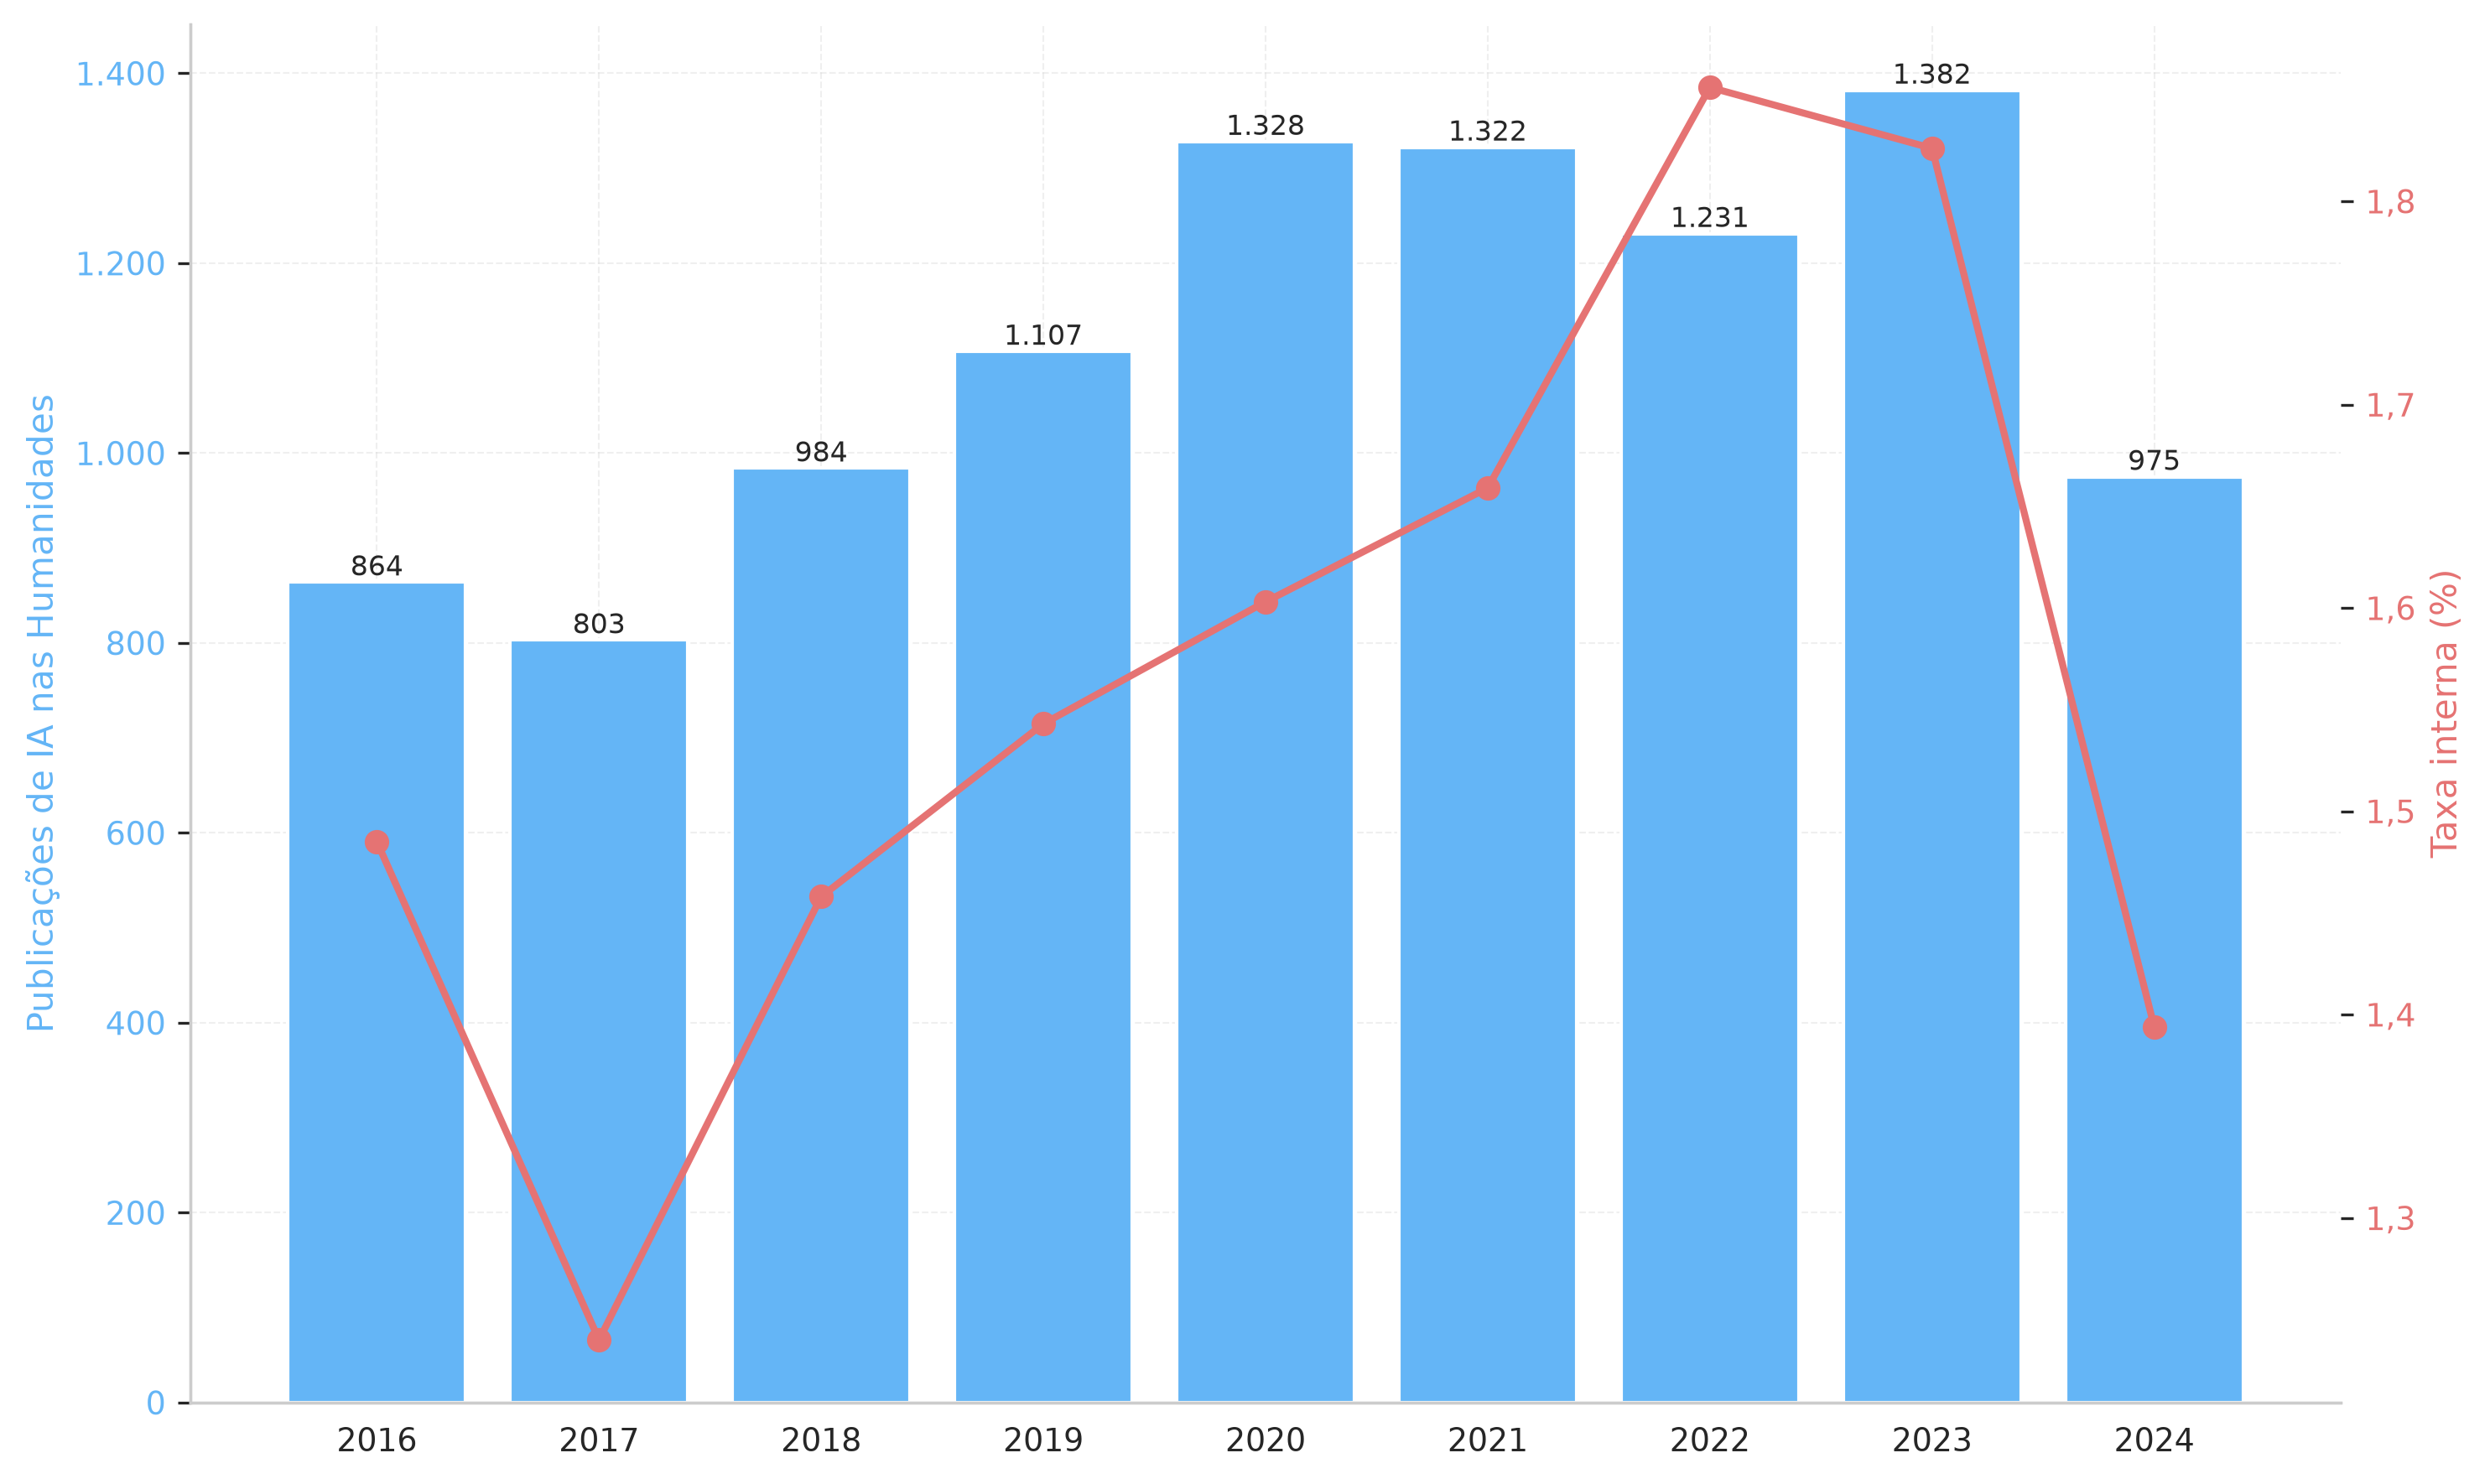
\includegraphics[width=0.85\linewidth]{figuras/cap.2/openalex_03_brasil_temporal.png}
    \caption[Evolução da produção brasileira de IA nas Humanidades, \texttt{OpenAlex} 2016--2024]{%
        Brasil, no período 2016--2024, pela definição por conceito do
        \texttt{OpenAlex}. As bolinhas mostram o volume anual, isto é, o número
        absoluto de obras de Humanidades que tocam a inteligência artificial, e
        a linha mostra a taxa interna, a fração que essas obras representam
        dentro de todas as obras de Humanidades do país no mesmo ano. O volume
        cresce de 864 obras em 2016 para 1.382 em 2023, ao passo que a taxa
        interna se mantém em uma faixa estreita, entre 1,24\% e 1,86\%, com pico
        em 2022. O descompasso entre os pontos que sobem e a linha que não
        acompanha é a leitura central da figura: o Brasil produz mais obras de
        inteligência artificial nas Humanidades a cada ano, sem que a fração das
        Humanidades dedicada ao tema se amplie na mesma medida. A retração
        aparente de 2024, com 975 obras, deve-se com grande probabilidade à
        indexação ainda incompleta do ano na plataforma, e não a um declínio
        real, limitação análoga à que afeta a própria base do \texttt{CSET}.
        Elaboração própria a partir do \texttt{OpenAlex}. Repositório com dados,
        \emph{scripts} e figuras em \protect\url{https://github.com/julianehelanski/bibliometria-ia-humanas}.}
    \label{fig:openalex_brasil_temporal}
\end{figure}

A trajetória brasileira no tempo, na Figura~\ref{fig:openalex_brasil_temporal}, mostra crescimento sustentado entre 2016, com 864 obras, e 2023, com 1.382, acompanhado de uma taxa interna que se move em uma faixa estreita, entre 1,24\% e 1,86\%, com pico em 2022. Leio a queda aparente de 2024, com 975 obras, com cautela, porque o \texttt{OpenAlex} segue indexando as publicações do ano mais recente, de modo que o número está quase certamente subestimado, do mesmo modo que a base do \texttt{CSET}. O que é marcante na curva é a estabilidade da taxa interna em um patamar baixo, e não a flutuação de cada ano: o volume cresce, e a fração das humanidades brasileiras que incorpora a inteligência artificial permanece presa em torno de 1,5\%, o que sugere uma expansão concentrada em poucos nichos, em lugar de uma difusão ampla pelo campo. A aceleração que a \texttt{Capes} e a \texttt{SciELO} registram a partir de 2022 aparece, no \texttt{OpenAlex}, como crescimento de volume sem alargamento da fração, e essa diferença de leitura vem dos recortes distintos das três bases, pois a janela do \texttt{OpenAlex} começa em 2016 e cobre o mundo, ao passo que as duas brasileiras se concentram no quadriênio 2021--2024.

\begin{figure}[htbp]
    \centering
    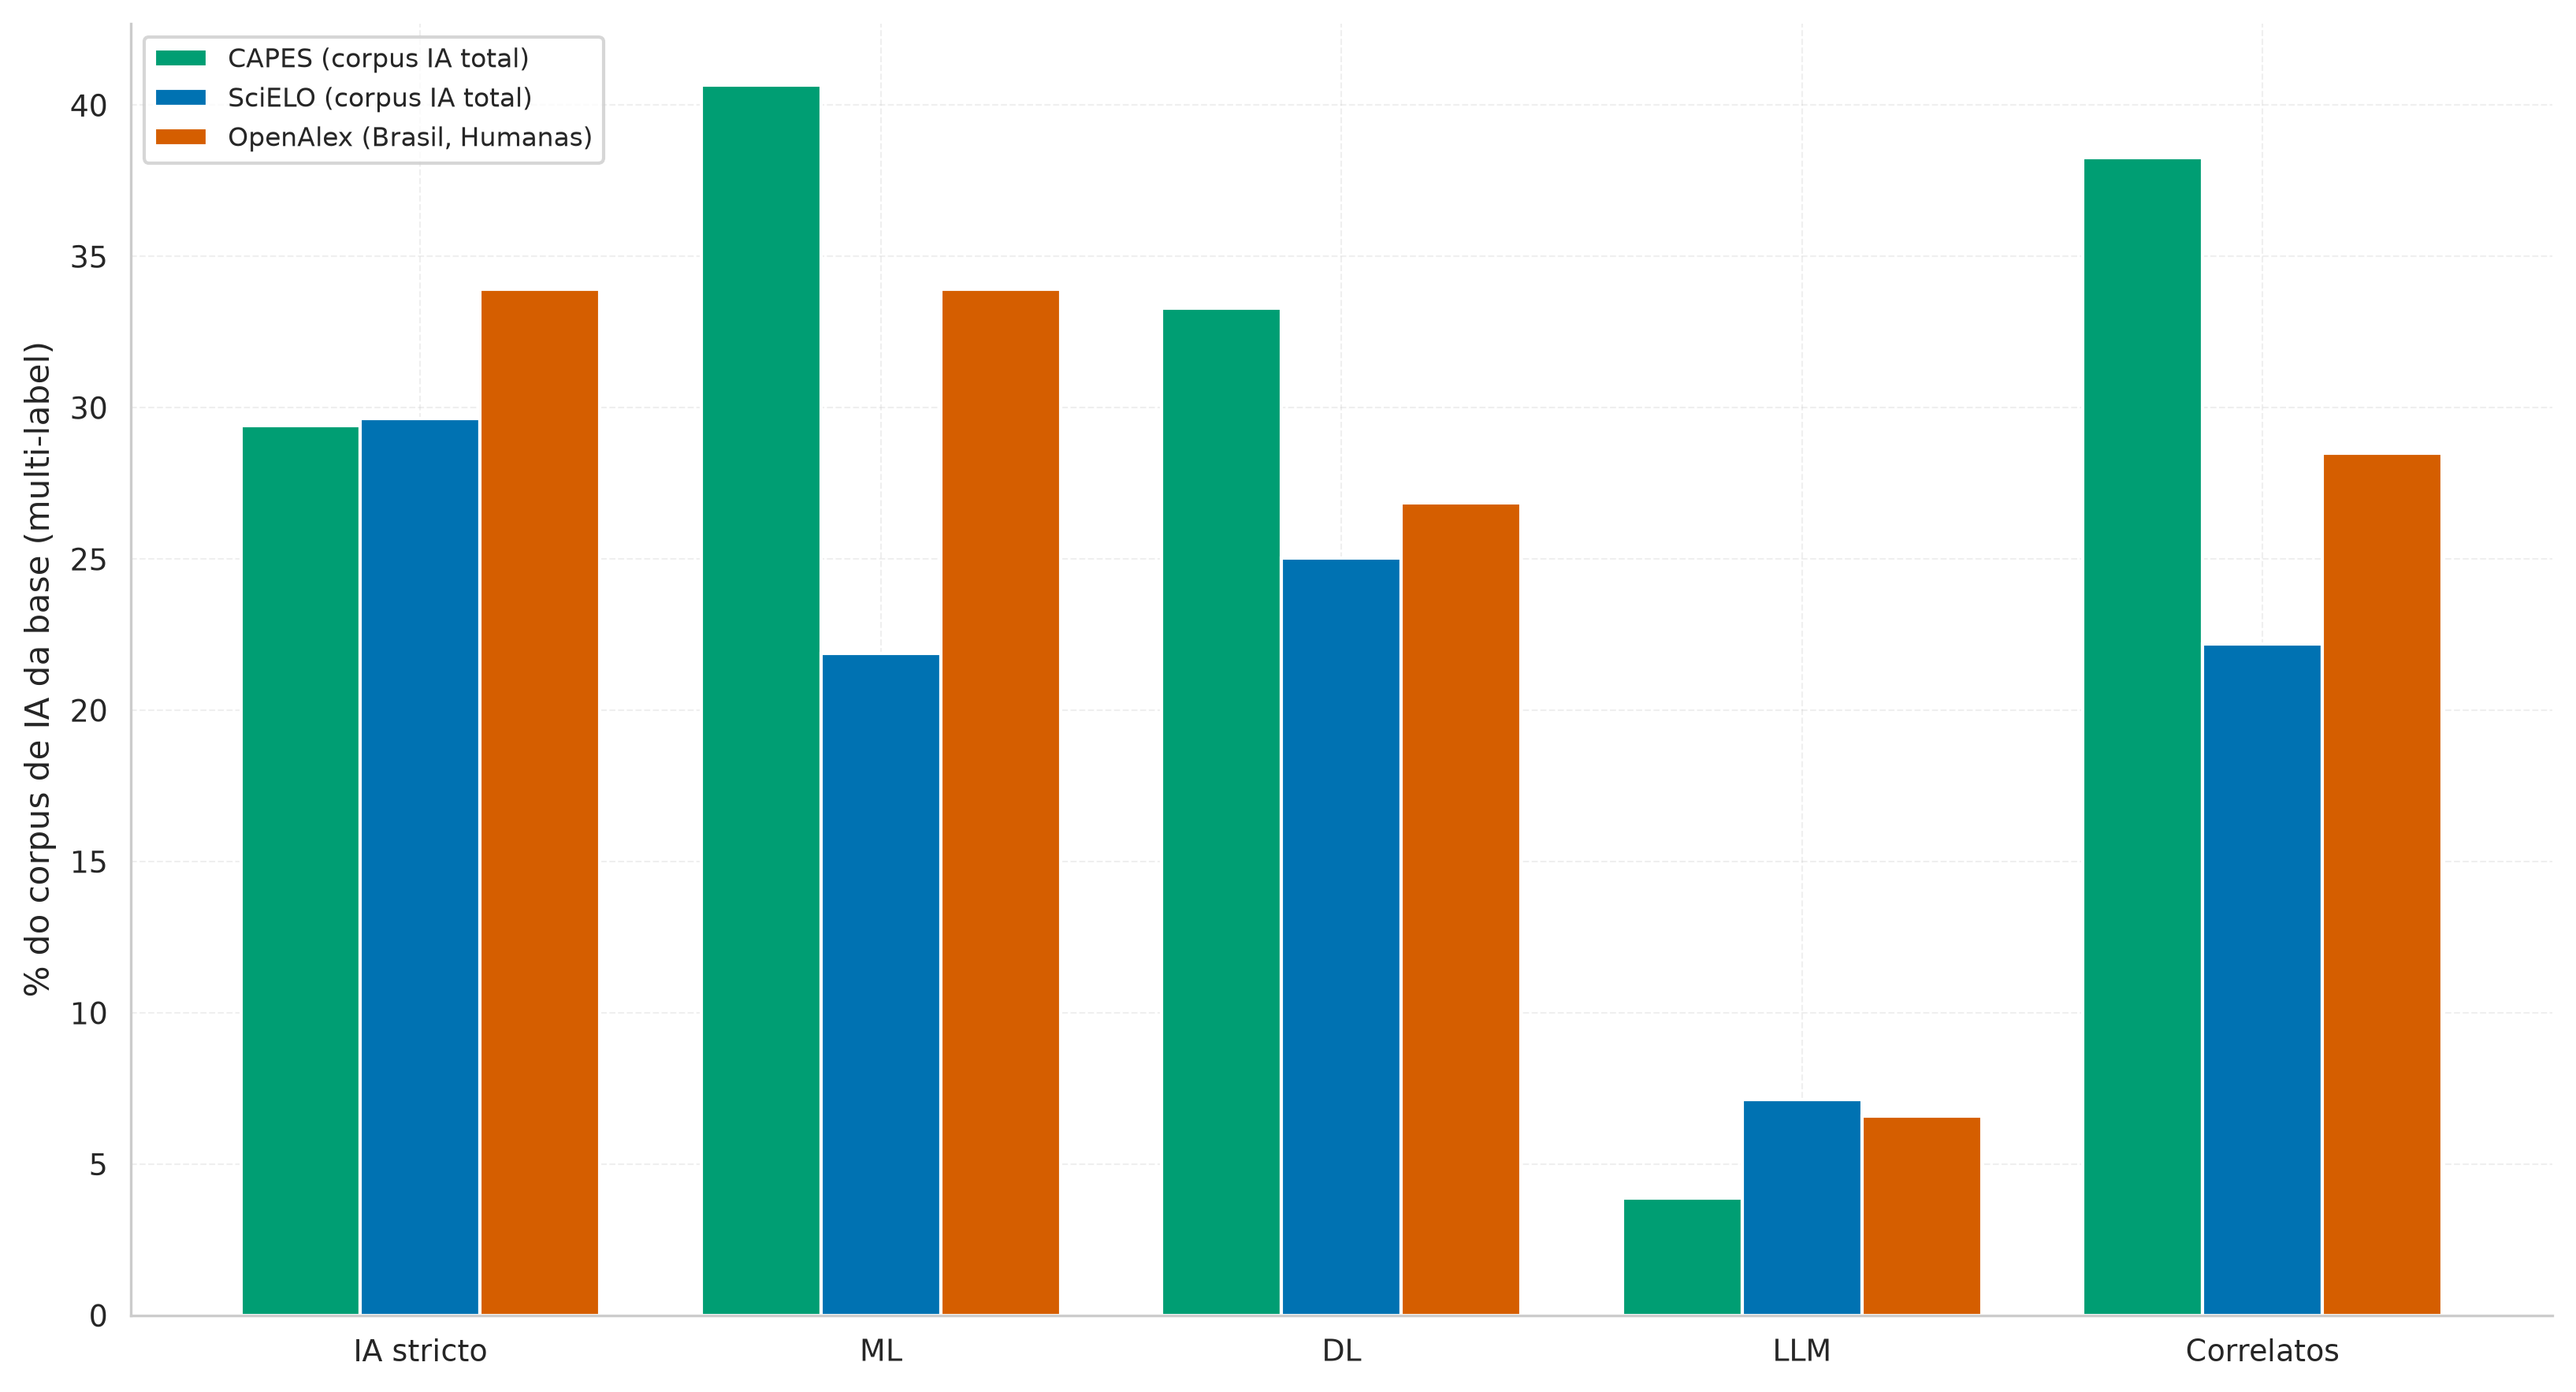
\includegraphics[width=0.85\linewidth]{figuras/cap.2/openalex_04_subcampos_3bases.png}
    \caption[Comparação dos subcampos de IA nas três bases]{%
        Peso relativo dos cinco subcampos da régua de classificação em cada uma
        das três bases. Um mesmo trabalho pode pertencer a mais de um subcampo,
        e por isso a soma dos percentuais ultrapassa cem. Os percentuais da
        \texttt{Capes} e da \texttt{SciELO} se referem ao corpus de inteligência
        artificial total de cada base, e os do \texttt{OpenAlex} ao recorte de
        Humanidades do Brasil pela régua de palavra-chave, e a diferença de
        escopo é declarada no corpo do texto. A hierarquia entre a inteligência
        artificial em sentido estrito e o aprendizado de máquina varia entre as
        três fontes, e os modelos de linguagem e a inteligência artificial
        generativa formam o menor subcampo nas três. Elaboração própria a partir
        do Catálogo de Teses e Dissertações da \texttt{Capes}, da \emph{API}
        ArticleMeta da coleção brasileira da \texttt{SciELO} e do
        \texttt{OpenAlex}. Repositório com dados, \emph{scripts} e figuras em \protect\url{https://github.com/julianehelanski/bibliometria-ia-humanas}.}
    \label{fig:openalex_subcampos_3bases}
\end{figure}

A Figura~\ref{fig:openalex_subcampos_3bases} põe lado a lado o peso dos cinco subcampos nas três bases, e a leitura pede uma ressalva de escopo, porque os percentuais da \texttt{Capes} e da \texttt{SciELO} vêm do corpus de inteligência artificial total de cada base, ao passo que os do \texttt{OpenAlex} vêm do recorte de humanidades do Brasil, pela régua de palavra-chave que torna os três comparáveis. Feita essa ressalva, dois padrões se destacam. O primeiro é que a hierarquia entre a inteligência artificial em sentido estrito e o aprendizado de máquina muda conforme a base, pois na \texttt{Capes} o aprendizado de máquina predomina, com 40,7\% contra 29,4\% da inteligência artificial em sentido estrito, na \texttt{SciELO} a relação se inverte, com 29,6\% contra 21,9\%, e no \texttt{OpenAlex} os dois subcampos empatam, com 33,9\% cada um, os mesmos 288 trabalhos. O segundo é que os modelos de linguagem e a inteligência artificial generativa formam, nas três bases, o menor subcampo, com 3,9\% na \texttt{Capes}, 7,1\% na \texttt{SciELO} e 6,6\% no \texttt{OpenAlex}, indício de que, no período que analiso, a virada generativa ainda não se traduzira em produção acadêmica de vulto nas humanidades, mesmo que já tivesse reorganizado o discurso público sobre a inteligência artificial.

As evidências do \texttt{OpenAlex}, tomadas em conjunto, levam o argumento desta seção para uma escala internacional. A marginalidade da inteligência artificial nas humanidades brasileiras não vem da escassez de produção humanística, porque o Brasil é o segundo maior produtor mundial do conjunto que analiso, e vem da estreita permeabilidade desse campo vasto às tecnologias de inteligência artificial, a menor entre os grandes produtores. Três ressalvas acompanham essa leitura. A primeira é que o \texttt{OpenAlex} privilegia os metadados em inglês, e por isso subestima a produção em português, e também a em chinês, o que afeta de modo desigual justamente o Brasil e a China; essa subestimação, porém, não fragiliza o achado, porque a \texttt{Capes} e a \texttt{SciELO} são bases nacionais, em português, sem viés de idioma, e devolvem a mesma ordem de grandeza baixa, de modo que o diagnóstico se sustenta exatamente onde a cobertura do \texttt{OpenAlex} falha. A segunda é que, na comparação por país, uma obra é somada uma vez para cada país de afiliação de seus autores, e os números brasileiros por obra única corrigem essa dupla contagem, ainda que as comparações internacionais a mantenham por alinhamento à regra do \texttt{CSET}. A terceira é que o ano de 2024 está subindexado. Nenhuma dessas ressalvas desfaz o achado de fundo, que três bases independentes, a \texttt{Capes}, a \texttt{SciELO} e o \texttt{OpenAlex}, reiteram por caminhos separados, e as três oferecem a possibilidade de retomar o levantamento futuramente e conferir o ritmo da emergência e refinar a categorização e a triagem que aqui apresentei.

A análise lexicométrica das três bases mede um campo cuja paisagem qualitativa tem percurso próprio, anterior ao adensamento recente que os números registram, e interpreto uma parte da escassez que elas medem como efeito de cobertura, dado que nenhum recorte bibliométrico, nem o da \texttt{Capes}, nem o da \texttt{SciELO}, nem o do \texttt{OpenAlex}, alcança a produção que circula em livros, capítulos e anais fora das bases indexadas. Há, porém, um limite mais profundo que o da cobertura, e que a bibliometria não tem como medir: ela conta o que se nomeia como inteligência artificial em um recorte recente, e por isso não enxerga o pensamento que vinha tratando a técnica sob outros nomes, a cibernética e o pós-humano, muito antes de a inteligência artificial se tornar o termo que organiza o debate. É a partir daqui que deixo de ler os números e passo a ler o terreno como ele se apresenta a mim, e reúno, à frente, os interlocutores que escolho para situar a minha pesquisa nessa tradição. Reconheço o primeiro deles em Laymert Garcia dos Santos, que, entre os primeiros a investigar sistematicamente as implicações políticas da tecnologia no Brasil, desenvolve desde os anos 1980 um percurso que vai da revolução cibernética ao pós-humano \parencite{Santos_2005_Entrevista, Santos_2022_SociologiaNaoAutocratica}. Seguindo a proposta de Garcia dos Santos uma ressonância que reencontro em trabalhos mais recentes como o de Diego Vicentin, que examina os desafios de aprofundar reflexões sobre inteligência artificial e de encontrar seu sentido ético pela noção de tecnologia de Gilbert Simondon em diálogo com os estudos críticos recentes sobre inteligência artificial \parencite{Vicentin_2022_Esboco}. A mesma preocupação atravessa as reflexões de Pedro Peixoto Ferreira sobre o que significa ser humano na era da inteligência artificial, pela análise do CAPTCHA (\textit{Completely Automated Public Turing Test To Tell Computers and Humans Apart}), em que ele sustenta que o CAPTCHA, ainda que nominalmente seja um sistema de segurança para distinguir humanos de computadores, funciona na prática como mecanismo de servidão maquínica e sujeição social, e recruta trabalho humano não remunerado para treinar sistemas de inteligência artificial das \textit{Big Techs} \parencite{Ferreira_2025_NaoSouUmRobo}.

A reflexão sobre as implicações éticas, estéticas e sociais das tecnologias de inteligência artificial aparece também em estudos antropológicos em diálogo com as artes visuais. Giselle Beiguelman investiga como a imagem digital, das \textit{selfies} aos \textit{memes}, dos \textit{deep fakes} à \textit{IoT}, tornou-se mediadora das relações sociais e campo de tensões políticas contemporâneas, e produz uma estética da vigilância impulsionada pela produção massiva de dados e imagens por meio de \textit{smartphones} \parencite{beiguelman2021}. Em diálogo com as artes visuais, Beiguelman usa inteligência artificial generativa (\texttt{DALL-E} e \texttt{Runway}) para criar imagens e vídeos que resgatam a história de mulheres e plantas estigmatizadas e proibidas ao longo do tempo, e toma a inteligência artificial como espaço de crítica e meio de problematização estética dos padrões de representação que os dados da tecnologia tendem a reproduzir \parencite{Beiguelman_2025_Venenosas}.\footnote{A exposição de Giselle Beiguelman pode ser visitada em: \url{https://venenosas.desvirtual.com}. Acesso em: 6 nov.~2024.} Dossiês de revistas acadêmicas acompanham esse movimento, e exploram as confluências entre pesquisa antropológica e interações entre humanos, transumanos e máquinas não humanas.\footnote{Iniciativa que aparece em dossiês de revistas como \enquote{Tecnopoéticas, Inteligência Artificial, maquinações e outras bricolagens}, cujos artigos exploram confluências e pontos de fricção entre pesquisa antropológica, processos narrativos e interações entre humanos, transumanos e máquinas não humanas \parencite{Magni_2024_Apresentacao}. Os artigos do dossiê estão disponíveis em: \url{https://seer.ufrgs.br/index.php/iluminuras/issue/view/5143}. Acesso em: 6 nov.~2024.}

A popularização da inteligência artificial generativa a partir de 2022 funcionou como vetor de atenção para as ciências sociais, e o que antes circulava em áreas especializadas tornou-se objeto de uso cotidiano, e ampliou o escopo das perguntas sobre o que são essas tecnologias e suas implicações para a sociedade. Trabalhos recentes abordam a propagação de \textit{deep fakes} e \textit{fake news}, as desigualdades socioeconômicas intensificadas pela inteligência artificial na educação, a análise psicanalítica da pós-humanidade e a xenoantropologia das máquinas como perspectiva para enfrentar a fusão das fronteiras entre espécies e artefatos.\footnote{A presença da tecnologia como objeto de debate pode ser aferida pela programação dos principais eventos das ciências sociais brasileiras e do Mercosul. Na XV Reunião de Antropologia do Mercosul (RAM), realizada em Salvador em agosto de 2025, com aproximadamente 178 grupos de trabalho, apenas 1 nomeia inteligência artificial diretamente no título: o GT~146 (\enquote{Perspectivas antropológicas sobre plataformas digitais, extrativismo de dados e inteligência artificial}, coordenado por Carolina Parreiras, Patricia Pereira Pavesi e Cecilia Melella); outros 10 GTs abordam tecnologia, digital ou dados de modo mais amplo, entre os quais o GT~023 (\enquote{Antropologia Digital e Tecnologias Contemporâneas}), o GT~011 (\enquote{Antropologia da ciência e da tecnologia em perspectiva}), o GT~027 (\enquote{Antropologia dos dados e das práticas de quantificação}) e o GT~078 (\enquote{Digitalización de la vida cotidiana y producción de conocimiento en América Latina}); 3 mesas redondas e 1 oficina completam esse escopo, entre as quais a MR~61 (\enquote{Pesquisa e redes sociais em tempos de \textit{TechBros} e Tecnofascismos: perspectivas feministas}) e a OF~37 (\enquote{Tecnologia, natureza, imaginação e trabalho abstrato: sistemas ciberfísicos como exemplo para uma teoria e prática críticas nos estudos sociotécnicos}). No 49º Encontro Anual da ANPOCS, realizado na \texttt{Unicamp} em outubro de 2025, com 68 grupos de trabalho e 31 mesas redondas presenciais, 1 GT e 1 mesa redonda nomeiam inteligência artificial diretamente: o GT~56 (\enquote{Inteligência Artificial, Sociedade, Cultura e Poder}) e a MR~20 (\enquote{Plataformas Digitais, IA e Sociedade: Desafios para as Ciências Sociais}); outros 5 GTs abordam tecnologia e plataformas digitais, entre os quais o GT~61 (\enquote{Pesquisa social com mídias e plataformas digitais}) e o GT~11 virtual (\enquote{Estudos Sociais da Ciência e da Tecnologia}). Na 35ª Reunião Brasileira de Antropologia (RBA), realizada em Goiânia em julho de 2026, com aproximadamente 118 grupos de trabalho, 73 mesas redondas e 24 simpósios especiais, nenhum espaço nomeia inteligência artificial diretamente no título; 4 GTs abordam tecnologia e o digital: GT~015 (\enquote{Antropologia da Técnica}), GT~017 (\enquote{Antropologia das ciências, tecnologias e outras ancestralidades}), GT~020 (\enquote{Antropologia digital e políticas etnográficas}) e GT~021 (\enquote{Antropologia digital: debates teóricos, metodológicos, éticos e políticos}); 2 simpósios especiais tratam de digitalização e algoritmos: SE~09 (\enquote{Entre pluralidade de saberes, descolonização e algoritmos}) e SE~11 (\enquote{Fazer e comunicar antropologia em tempos de plataformas e digitalização}); e 1 mesa redonda aborda o subcampo: MR~63 (\enquote{Perspectivas e caminhos da antropologia digital no Brasil}). As programações completas estão disponíveis em: \url{https://www.xvram.com.br} (acesso em: 5 abr.~2026), \url{https://anpocs.org.br/49-encontro-anual} (acesso em: 5 abr.~2026) e \url{https://www.rba2026.com.br} (acesso em: 5 abr.~2026).}

A produção de \enquote{etnografias do digital}\footnote{Tema da edição 68, v.~30 da \textit{Revista Horizontes Antropológicos} organizada por Jean Segata, Theophilos Rifiotis e Maria Elisa Máximo. A edição está disponível em: \url{https://seer.ufrgs.br/index.php/horizontesantropologicos/issue/view/5110/1484}. Acesso em: 6 nov.~2024.} acompanhou esse movimento de expansão, e expõe a diversidade de análises do digital e a sua presença na vida cotidiana. As ciências sociais vêm questionando a ideia de sociedade como reunião apenas de humanos, e consideram coletivos formados por moléculas, códigos binários e dados algoritmicamente minerados, tecnologias que, ainda que globais em alcance, encontram resistências e se transformam em práticas locais. Computadores, \emph{softwares}, aplicativos, redes sociais, algoritmos, DNA, inteligência artificial e organismos geneticamente modificados formam um amálgama que costura tecnologias digitais e da vida, e desenham mundos múltiplos e futuros já presentes, ainda que desigualmente distribuídos \parencite{Rifiotis2024Etnografias}. Essa paisagem qualitativa não contradiz a escassez que as três bases medem, e a precede e a contextualiza, porque mostra que a antropologia brasileira vinha pensando a técnica e o digital muito antes de a inteligência artificial se tornar objeto de estudo desta tese, de artigo e de grupo de trabalho. A defasagem que a bibliometria registra é, então, menos a ausência de um pensamento sobre a tecnologia e mais como que esse pensamento se volta para a inteligência artificial como tema de pesquisa. É nessa dobra que situo a minha pesquisa, entre uma tradição que já existe e um objeto de estudo ainda em emergência.

\section{Arremate: figurações e análise computacional}
\label{sec:revisao_etnografia}

Abri o capítulo~\ref{capitulo2} com duas epígrafes e duas figuras postas lado a lado, a do exército de aliados de Latour e a do berço de gato de Haraway, porque em Haraway a figuração propõe e põe em jogo padrões. Os padrões são formas que emergem da relação e que pedem resposta, e obrigam a fazer algo com elas. Exigem receber e passar, pegar e largar, e por isso são coletivos e relacionais, e podem ser jogados tanto por humanos quanto por não humanos, desde que o ritmo entre dar e receber se mantenha. Porque propõem jogos, esses padrões são mais propositivos do que descritivos, e apresentam modos possíveis de relação, aquilo que \textcite{Haraway2023Ficar} chama de tornar-se-com e fazer-com, a simpoiese. É essa dupla natureza que separa a figuração de Haraway da figuração militar de Latour. O exército de aliados descreve como a tecnociência funciona, ao passo que o jogo da figura de barbante descreve como ela funciona e, no mesmo gesto, propõe que poderia funcionar de outro modo. Pôr as duas figuras em relação é, ele mesmo, um gesto de figurar, o de passar um fio de uma mão a outra para ver que forma se sustenta entre elas \parencite[p.~25]{Haraway2023Ficar}. As duas dão a ver, portanto, duas maneiras de pôr as coisas em relação no fazer-conhecimento: de um lado, o autor cercado de aliados, em que a relação acumula reforços e se mede pela controvérsia que vence; de outro lado, as mãos entrelaçadas por um fio compartilhado, em que a relação só persiste enquanto há quem a receba e devolva, sem \textit{front} e sem adversário.

Convocar autores e alistá-los para sustentar uns argumentos, contestar outros e acumular reforços contra o ataque deriva das figurações que \textcite[cap.~1]{Latour2011CienciaEmAcao} elaborou para explicar a produção tecnocientífica, ao lado de outras figurações menos confrontativas. Escolhi ficar com as figurações de \textcite{latour_woolgar_1986_lab_life} e \textcite{latour1996clarifications, Latour1999RecallingANT, Latour1987Science, Latour1999PandorasHope, Latour2013Inquiry}, ao lado das figurações de Haraway e de Stengers, que tomam o conhecimento como prática de pôr as coisas em relação por outros caminhos, a trama multiespécie e a desaceleração do pensamento. Justifiquei nessa abertura o recorte do corpus, e expliquei que o recorte antecede a análise lexicométrica em vez de ser montado para ela, porque a figuração militar-industrial já era objeto da pesquisa antes disso, sustentada pela leitura e pelo uso desses termos na construção da tese, e a análise veio depois, para dar base à leitura interpretativa que eu já vinha fazendo. É essa tensão entre alistar e tecer que levo adiante, não para resolvê-la, mas a partir dela, tramar com as figurações da/na tecnociência nos capítulos seguintes.

A seção~\ref{sec:analise_lexicometrica} apresentou a análise lexicométrica das figurações, que desenvolvi com o \texttt{claude} e o \texttt{claude code} sobre seis obras de Latour publicadas entre 1986 e 2013. A análise lexicométrica abrangeu um conjunto de procedimentos que processa um corpus textual com métodos estatísticos e computacionais, identifica frequências, distribuições e relações de co-ocorrência entre as palavras, e preserva, pelo procedimento de \emph{keyword in context}, o vínculo de cada ocorrência com a sua vizinhança textual. O número de ocorrências de um rótulo foi o ponto de partida da análise. Organizei-a em três etapas, e a razão dessa divisão é que cada etapa pergunta o que acontece com as figurações quando muda o objeto que Latour descreve. A etapa~1 processou os três livros (\emph{Laboratory Life}, de Latour e Woolgar, de 1986, \emph{Science in Action}, de 1987, e \emph{Pandora's Hope}, de 1999) e mediu a densidade do rótulo \texttt{militar} em cada um deles. A densidade é baixa em \emph{Laboratory Life}, salta em \emph{Science in Action} e permanece alta em \emph{Pandora's Hope}. Dessa forma, a análise textual forneceu um outro contexto que complementou a leitura e as aplicações que eu vinha fazendo das obras nesta tese. A etapa~2 estendeu a análise aos dois artigos metateóricos (\emph{Clarifications}, de 1996, e \emph{On Recalling ANT}, de 1999), e fiz isso porque, se o vocabulário militar satura a escrita com que Latour descreve a tecnociência, era razoável esperar que ele se reorganizasse quando Latour, de modo autorreflexivo, reinterpreta a própria teoria; o que a análise mostrou foi a queda do rótulo \texttt{militar} e a dominância dos rótulos \texttt{topologia} e \texttt{textil}, que acrescentei ao catálogo justamente para captar o vocabulário têxtil-topológico que a leitura qualitativa desses dois artigos havia revelado. A essa etapa somei uma validação amostral semântica, em que classifiquei ocorrência a ocorrência em uso figural, parcialmente figural ou não-figural, para distinguir o uso figurativo do uso polissêmico ou citacional e sustentar a inversão de registro já no plano figural depurado, e não apenas no plano lexical bruto. A etapa~3 processou \emph{An Inquiry into Modes of Existence}, de 2013, obra em que apliquei dois catálogos em paralelo, e registrou a reentrada moderada do vocabulário militar agora articulado a objetos cosmopolítico-diplomáticos, com a pendência declarada da desambiguação refinada das suas ocorrências. A subseção~\ref{subsec:costurando_figuracoes} reuniu o que as três etapas mostram: a figuração militar-industrial é uma figuração situada, que aparece de modo seletivo conforme o objeto descrito, e o vocabulário têxtil-topológico, que reconheço como figuração feminista a partir de Haraway, é uma figuração que o próprio Latour compõe nos seus momentos autorreflexivos.

Entre a análise lexicométrica e o mapeamento bibliométrico, percorri as leituras que atravessei ao longo do doutorado, e as dispus na ordem em que cada problema empírico do meu campo as convocou. A seção~\ref{sec:estudos_ciencia_tecnologia} situou a pesquisa nos estudos sociais da ciência e da tecnologia e nos estudos do digital, e marquei ali a tradição antropológica da técnica que corre em paralelo à genealogia sociológica do campo, de Mauss e Lévi-Strauss à filosofia da técnica de Simondon e Hui, além do princípio de não-centramento no digital de Pink, Horst e Postill, que tomo como recorte do objeto. A seção~\ref{sec:etnografias_ia_mediacao} reuniu as primeiras pesquisas antropológicas e sociológicas sobre inteligência artificial, a antropologia de Diana Forsythe e a sociologia dos sistemas especialistas de Harry Collins, e desenvolveu o conceito de mediação técnica que Latour formula em \emph{Pandora's Hope}, revisitado à luz dos sistemas de inteligência artificial generativa; fiz esse percurso porque é o conceito de mediação técnica que me permite descrever o \texttt{claude} e o \texttt{claude code} como actantes que se transformam e transformam os modos de produção tecnocientíficos, de fazer-conhecimento. A seção~\ref{sec:predicao_poder} fez um apanhado das genealogias críticas do poder tecnológico, de Kate Crawford a Matteo Pasquinelli e Vladan Joler, em diálogo com as inflexões brasileiras dessas perguntas, e firmou a postura de descrição que sustento, a de descrever as redes da inteligência artificial sem afundar na denúncia que só vê extração nem na celebração que só vê solução. 

A seção~\ref{sec:emergencia_campo_brasileiro} apresentou o mapeamento bibliométrico do campo brasileiro de estudos em inteligência artificial nas ciências humanas e sociais, que fiz com o \texttt{claude} e o \texttt{claude code} sobre três bases, o Catálogo de Teses e Dissertações da \texttt{Capes}, a coleção brasileira da \texttt{SciELO} e a base internacional \texttt{OpenAlex}. Tomei a \texttt{Capes} como base principal porque um campo em formação inscreve-se primeiro na pós-graduação, na tese e na dissertação, e complementei a sondagem com a \texttt{SciELO} e com o \texttt{OpenAlex} para confrontar o recorte nacional com o periódico e com o recorte internacional. Por busca padronizada de termos-chave, categorização do material retornado em subcampos e leitura situada dos dados, o mapeamento registrou em forma quantificada uma emergência tardia e tematicamente deslocada dos estudos brasileiros sobre inteligência artificial, e estudos sobre tecnologia em geral, marginalidade que se confirma da pós-graduação ao periódico e do recorte nacional ao internacional, e que interpreto menos como ausência de pensamento sobre a tecnologia e mais como uma defasagem do vocabulário com que esses estudos delimitam a inteligência artificial e tecnologias correlatas do mesmo universo. Esse mapeamento surgiu da necessidade de situar esta tese e de mensurar os modos e os ritmos pelos quais a área se aproxima da inteligência artificial como tema e objeto de estudo.

As duas linhas de trabalho deste capítulo~\ref{capitulo2} entregam para os capítulos seguintes três coisas que serão retomadas. A primeira é o reconhecimento de que a figuração com que se descreve a tecnociência é parte do que se descreve, e por isso o tratamento das figurações na obra de Latour, Latour e Woolgar (e também com Haraway e Stengers) como objetos etnográficos, que desenvolvi com o \texttt{claude} e o \texttt{claude code}, abre o caminho que os capítulos~\ref{capitulo3} e~\ref{capitulo4} repetem em outras escalas. A segunda é a tensão entre alistar e aliar, que percorre este capítulo no plano da composição da literatura e que se redistribui, nos próximos capítulos, no plano da composição do campo: alistar aliados teóricos é gesto homólogo ao que Fábio e Cláudio fazem para sustentar o \texttt{C4AI} e ao que Marcelo faz para sustentar o \texttt{Spira}, e descrever esse gesto teórica e empiricamente é parte do que a tecno-etnografia faz. A terceira é a posicionalidade não-inocente que essa tensão exige reconhecer, e a postura de descrição que dela decorre, a de ficar com o problema. O capítulo~\ref{capitulo3} investiga a rede que Fábio e Cláudio construíram ao longo de cinco anos de parceria \texttt{C4AI}-\texttt{IBM}, e a descreve pela sua extensão no tempo, da genealogia corporativa desde Hollerith, em 1890, à dissolução da parceria em dezembro de 2025; o capítulo~\ref{capitulo4} examina a rede que Marcelo construiu com o \texttt{Spira}, e a descreve pela densidade material da cadeia de translações que converteu a voz de pacientes com insuficiência respiratória em espectrogramas, coeficientes e artigos científicos. As duas redes são extensas, cada uma à sua maneira, e voltam a se cruzar no ponto em que a dissolução da parceria e a falha de generalização do modelo expõem a fragilidade do que parecia estável e a proximidade do que parecia distantes.

% ===== Inscrições \texttt{InfraNodus} / trajetória narrativa do capítulo 2 (inserido automaticamente — ajustar posição e prosa) =====
\medskip

A análise de rede textual deste capítulo, no mesmo procedimento descrito no capítulo~\ref{capitulo1}, produziu seis inscrições: três vistas sincrônicas da rede de co-ocorrência (rede completa, núcleo por \textit{degree} e núcleo por critérios informacionais) e três vistas diacrônicas da trajetória dos conceitos ao longo da leitura (Gantt lexical, fluxo aluvial e trajetória semântica), reunidas a seguir.

\begin{figure}[H]
\centering
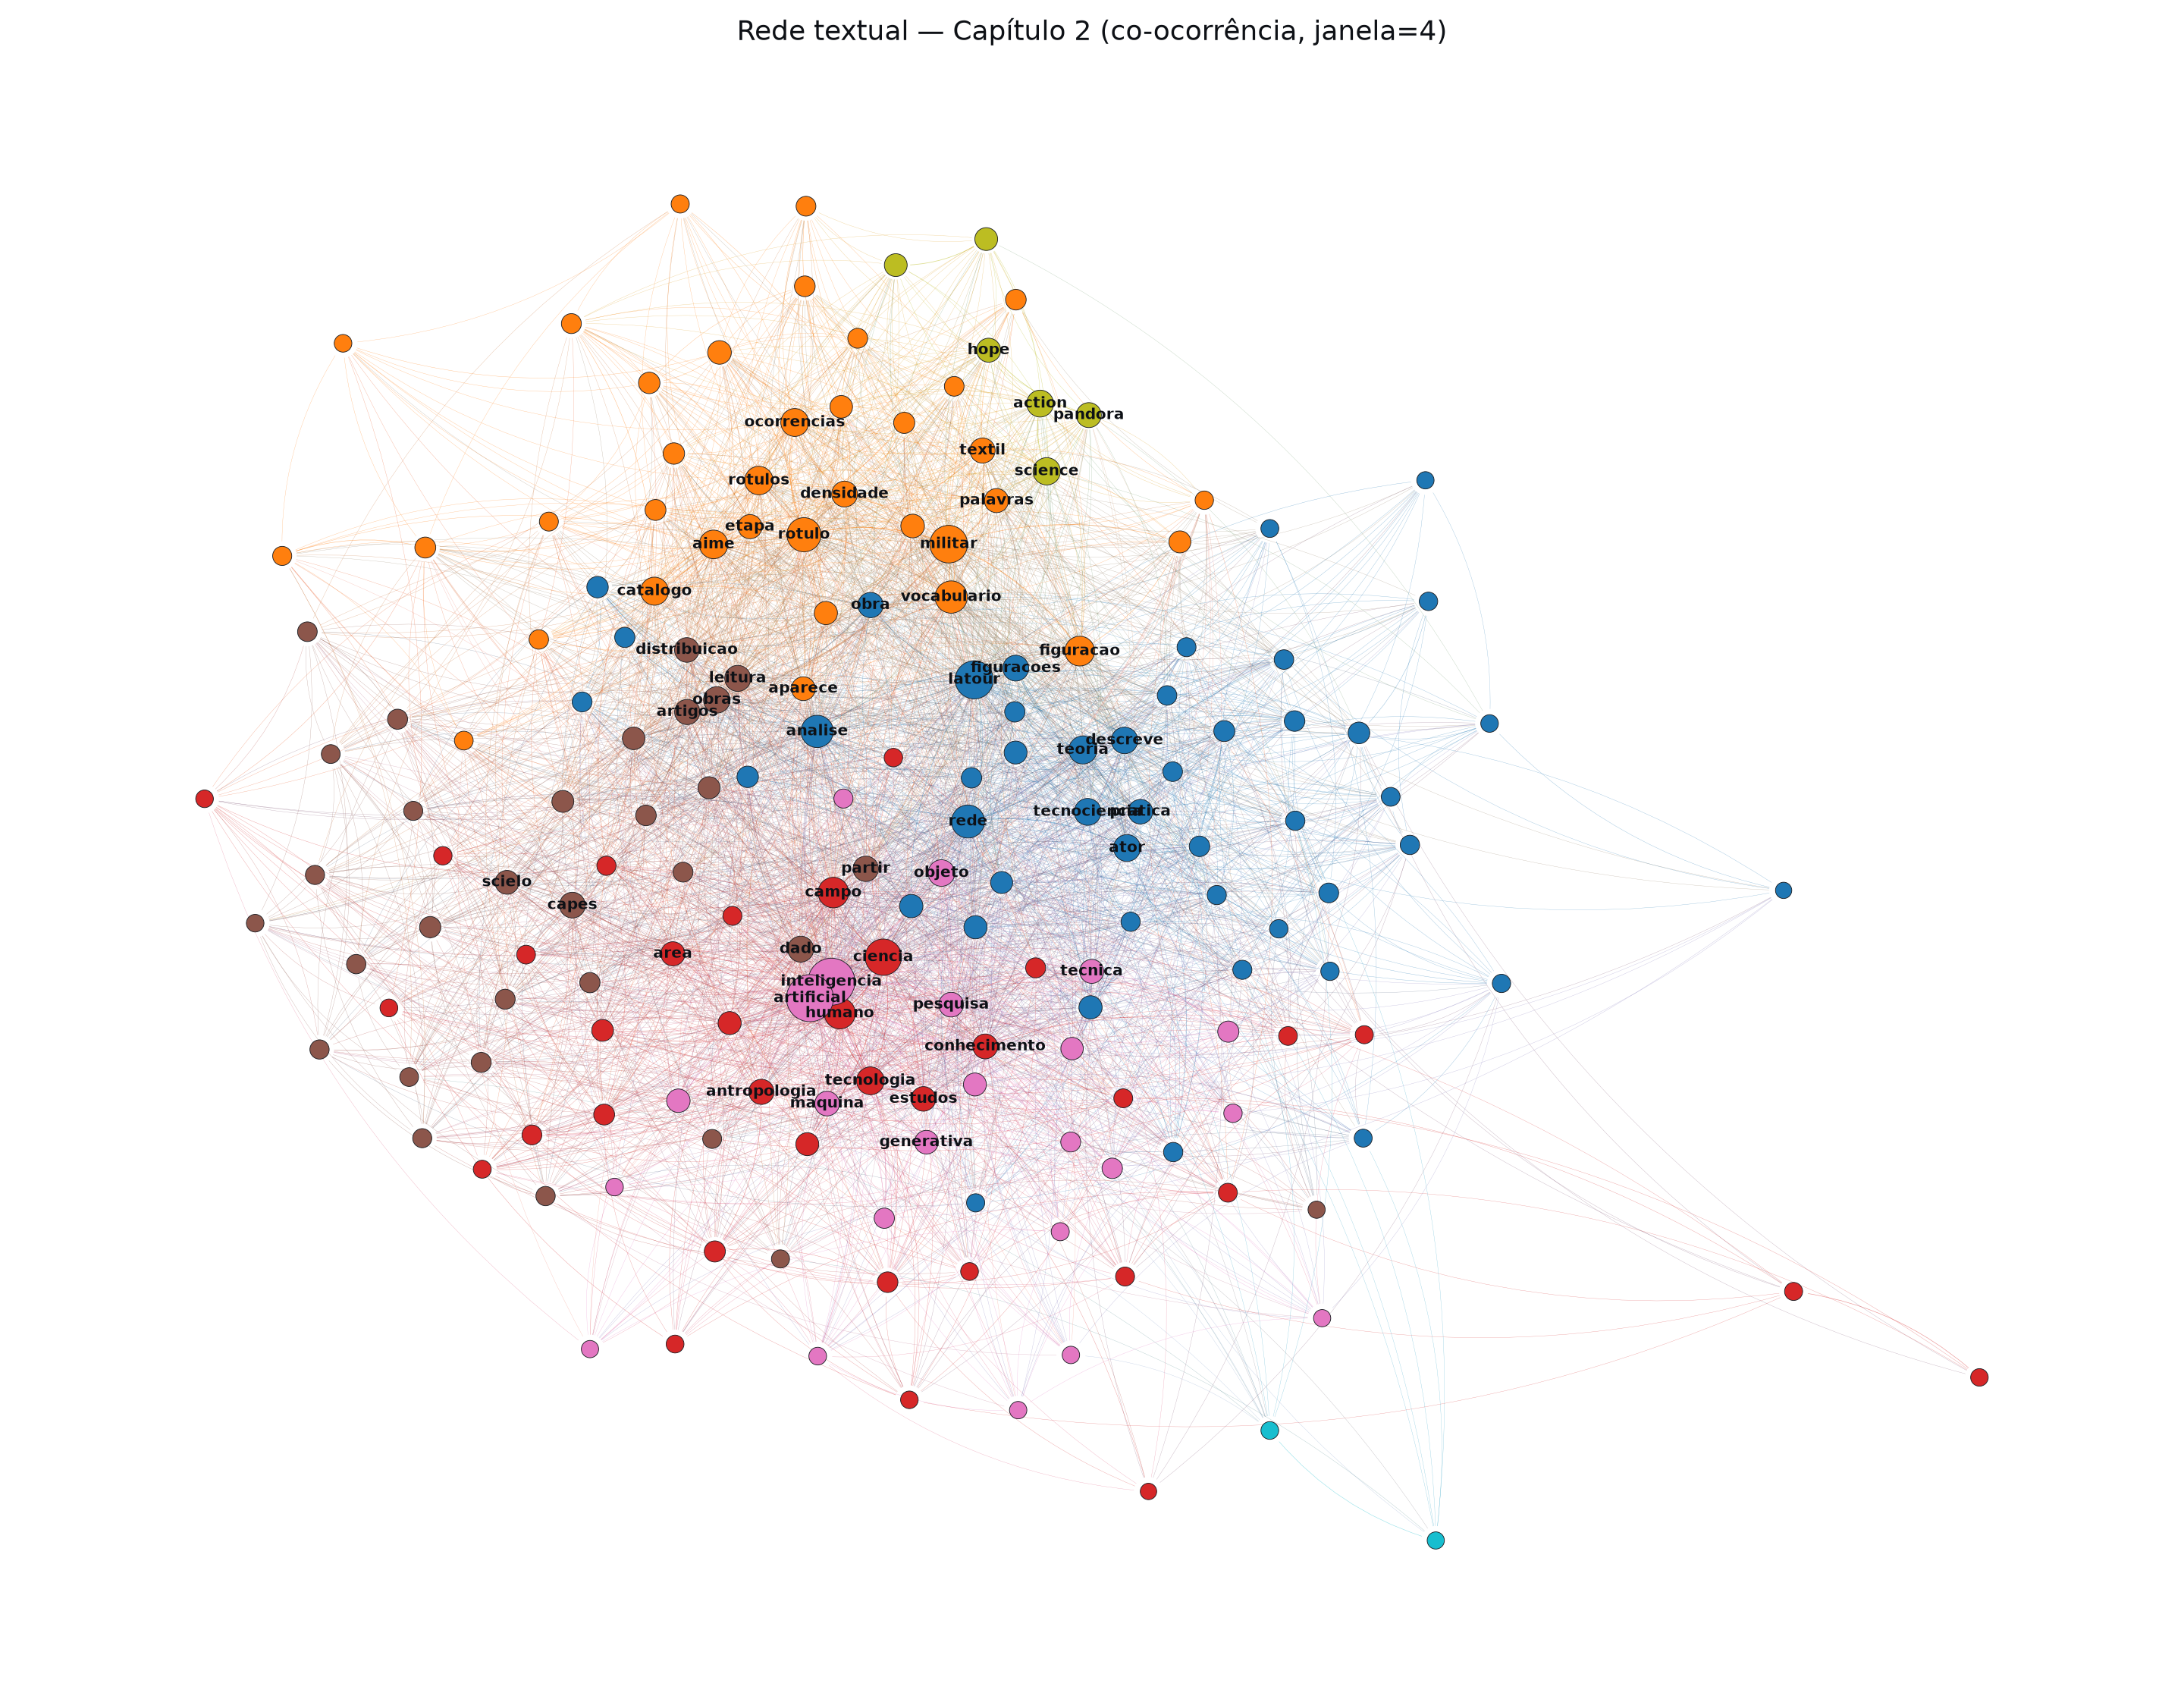
\includegraphics[width=1.0\textwidth,keepaspectratio]{figuras/cap.2/infranodus_cap2_network.png}
\caption[Rede textual completa do capítulo~\ref{capitulo2} (análise de rede textual)]{Rede textual completa do capítulo~\ref{capitulo2}. O grafo resulta de janela deslizante de 4 \textit{tokens} sobre o texto pré-processado (remoção de \textit{stopwords}, comandos \LaTeX, lematização leve), com pesos decrescentes pela distância (3-2-1). Os nós são os 180 termos de maior frequência mantidos no maior componente conectado após a filtragem de arestas com peso $<2$; o tamanho do nó é proporcional ao \textit{degree} ponderado e a cor indica a comunidade detectada por Louvain ponderado; as arestas, arqueadas, recebem a mistura das cores das comunidades que ligam. Esta vista privilegia a estrutura geral do capítulo, incluindo termos periféricos e pontes entre tópicos. Arquivos auxiliares (\texttt{.gexf} para \texttt{Gephi}, CSVs, métricas e relatório) no repositório \url{https://github.com/julianehelanski/tecno-etnografia-centro-ia}.}
\label{fig:infranodus-cap2-network}
\end{figure}

\begin{figure}[H]
\centering
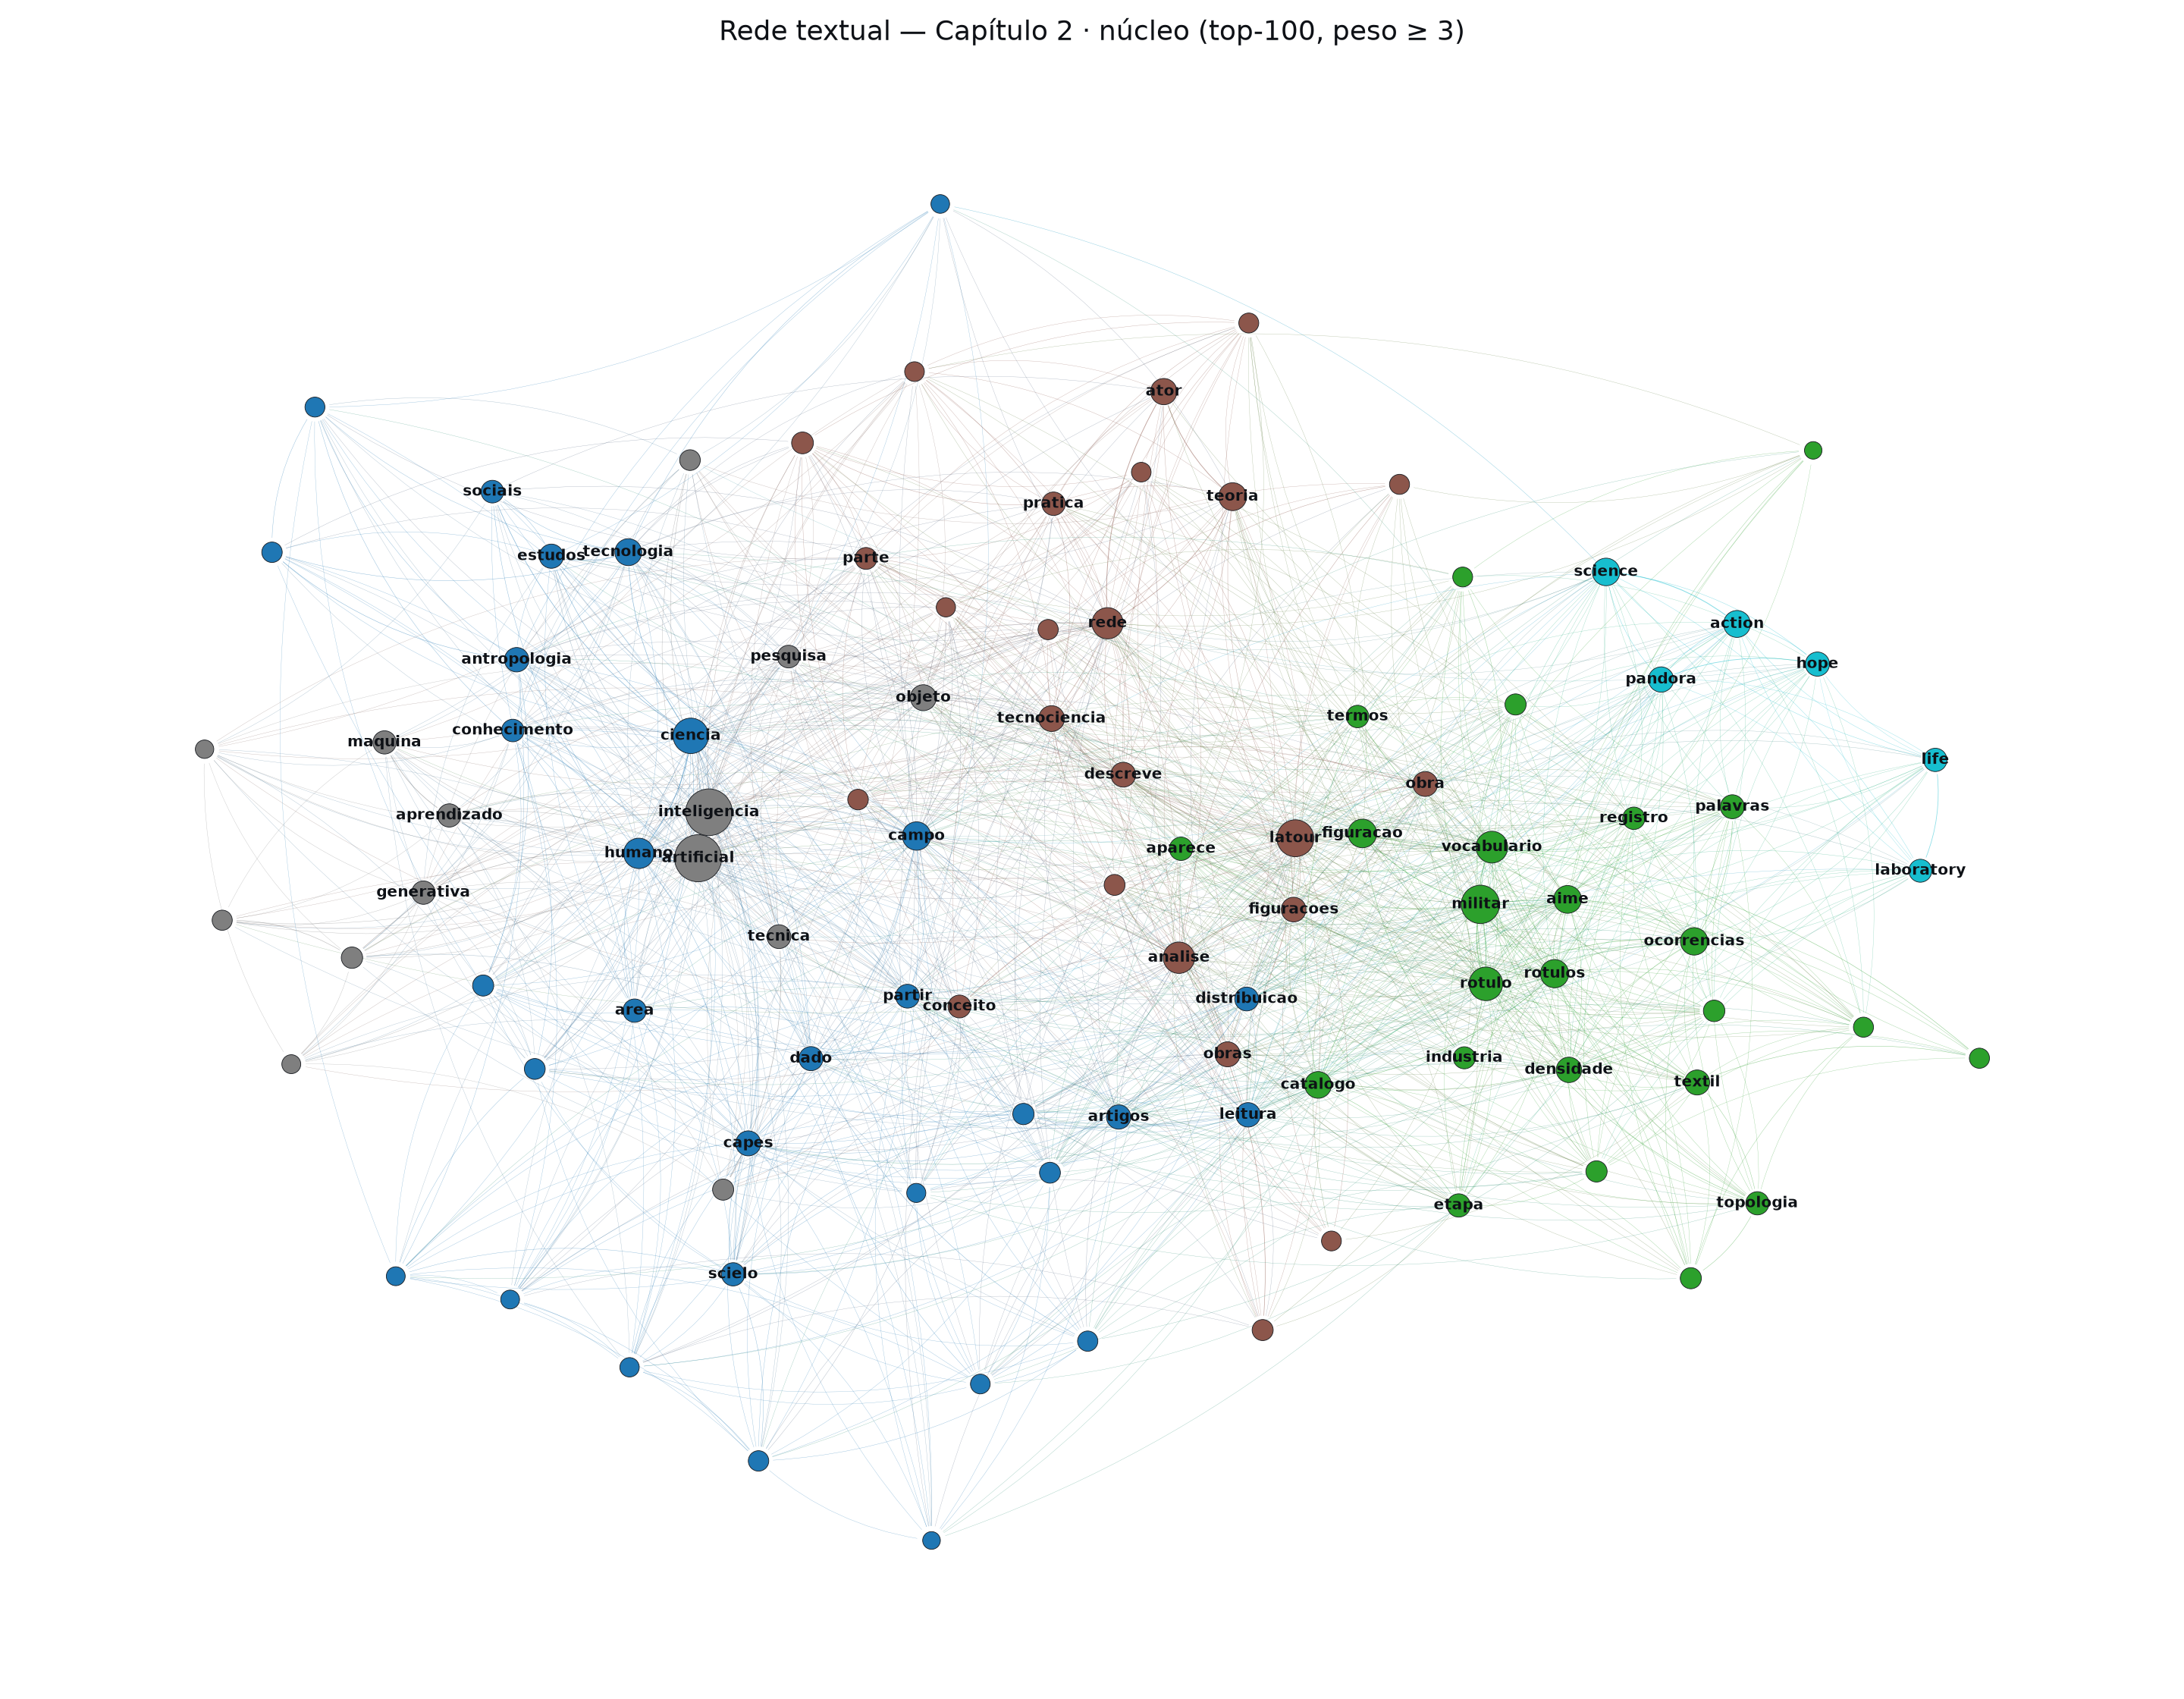
\includegraphics[width=1.0\textwidth,keepaspectratio]{figuras/cap.2/infranodus_cap2_focus.png}
\caption[Núcleo da rede textual do capítulo~\ref{capitulo2} (análise de rede textual)]{Núcleo da rede textual do capítulo~\ref{capitulo2} (análise de rede textual). Os nós são os 100 termos com maior \textit{degree} ponderado; o tamanho do nó é proporcional ao \textit{degree}; a cor indica a comunidade detectada por Louvain ponderado; as arestas, arqueadas, recebem a mistura das cores das comunidades que ligam (peso $\geq 3$). Comparada à figura~\ref{fig:infranodus-cap2-network}, esta vista retém apenas o esqueleto semântico do capítulo, ou seja, os conceitos mais centrais e suas conexões fortes, sem a periferia. Versão de alta resolução, arquivo \texttt{.gexf} para o \texttt{Gephi} e relatório completo disponíveis no repositório \url{https://github.com/julianehelanski/tecno-etnografia-centro-ia}.}
\label{fig:infranodus-cap2-focus}
\end{figure}

\begin{figure}[H]
\centering
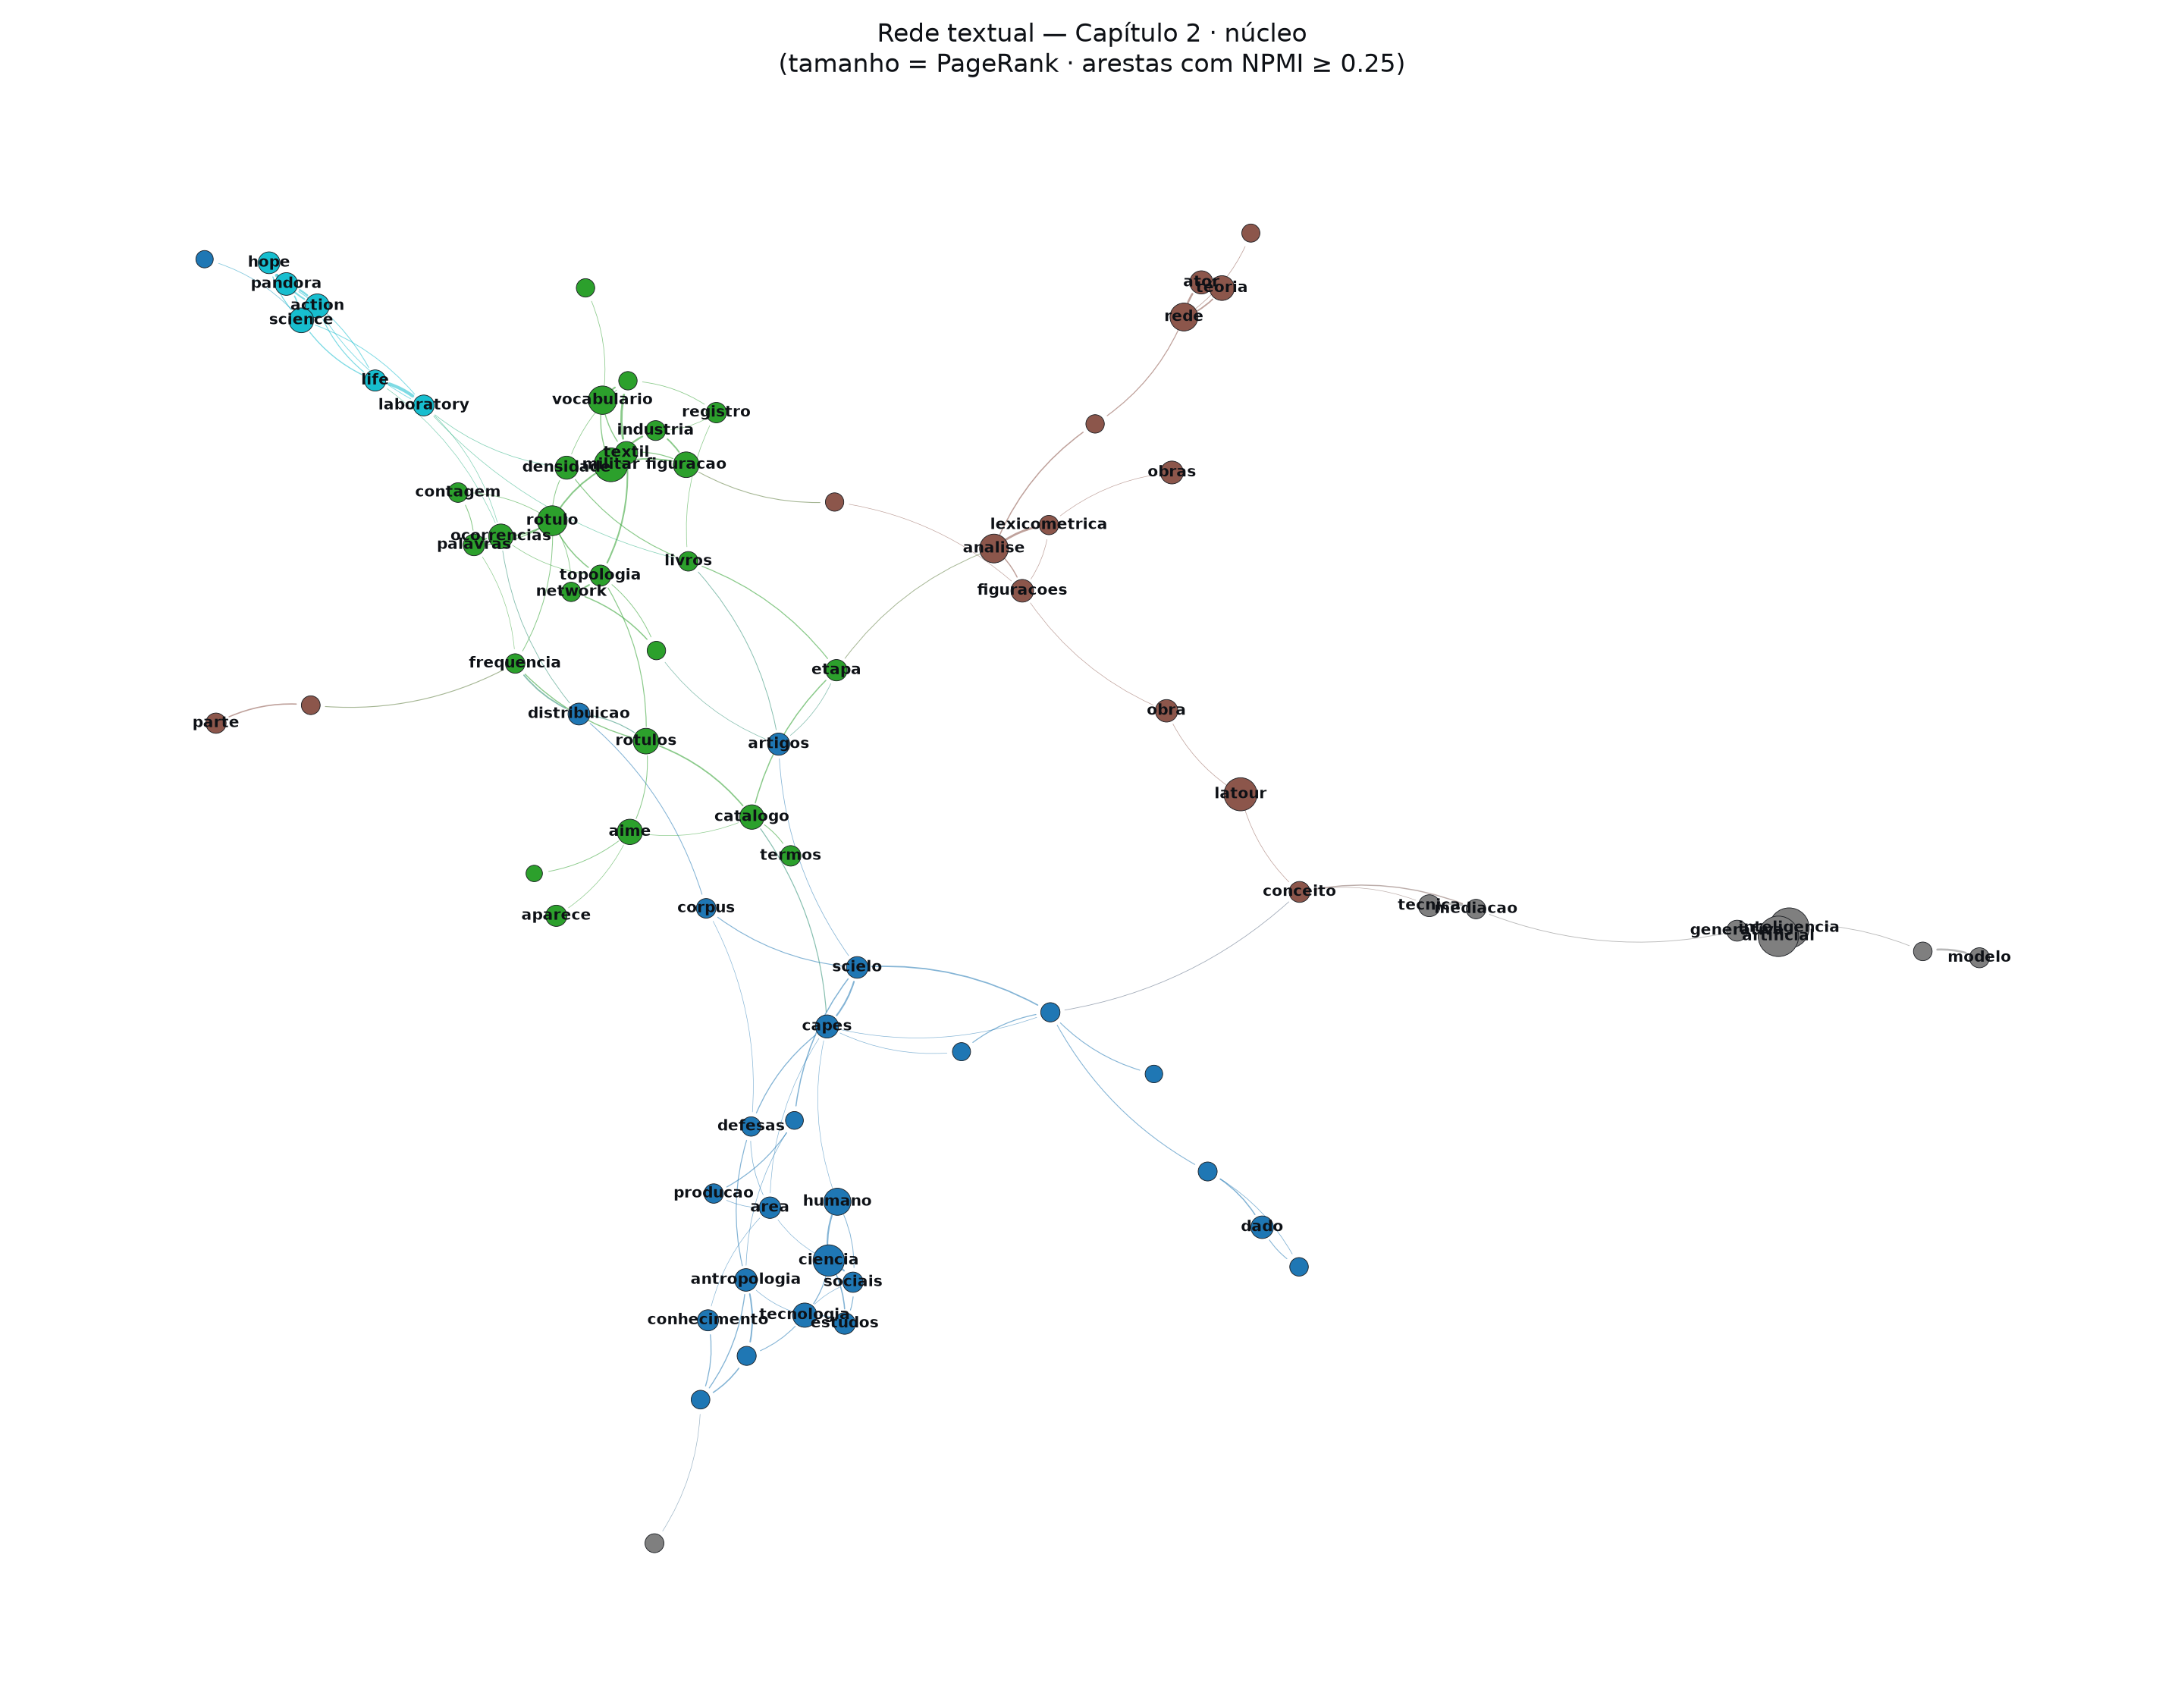
\includegraphics[width=1.0\textwidth,keepaspectratio]{figuras/cap.2/infranodus_cap2_focus_pmi.png}
\caption[Núcleo da rede textual do capítulo~\ref{capitulo2} ponderado por PageRank e NPMI]{Núcleo da rede textual do capítulo~\ref{capitulo2}, ranqueado por critérios informacionais em vez de frequentistas. Os mesmos 100 nós da figura~\ref{fig:infranodus-cap2-focus} são exibidos, mas o tamanho passa a ser proporcional ao \textit{PageRank} (centralidade na rede, em vez de contagem bruta) e as arestas são filtradas pelo \textit{Normalized Pointwise Mutual Information} (NPMI~$\geq 0{,}25$), retendo apenas co-ocorrências surpreendentes dadas as frequências marginais de cada termo. A cor mantém a comunidade Louvain, e as arestas, arqueadas, recebem a mistura das cores das comunidades que ligam. Esta vista promove conceitos pouco frequentes e estrategicamente posicionados, e deprime termos onipresentes cuja associação com qualquer outro é trivial, funcionando como contraponto à leitura puramente frequentista. Métricas e arquivo \texttt{.gexf} no repositório \url{https://github.com/julianehelanski/tecno-etnografia-centro-ia}.}
\label{fig:infranodus-cap2-pmi}
\end{figure}

\begin{figure}[H]
\centering
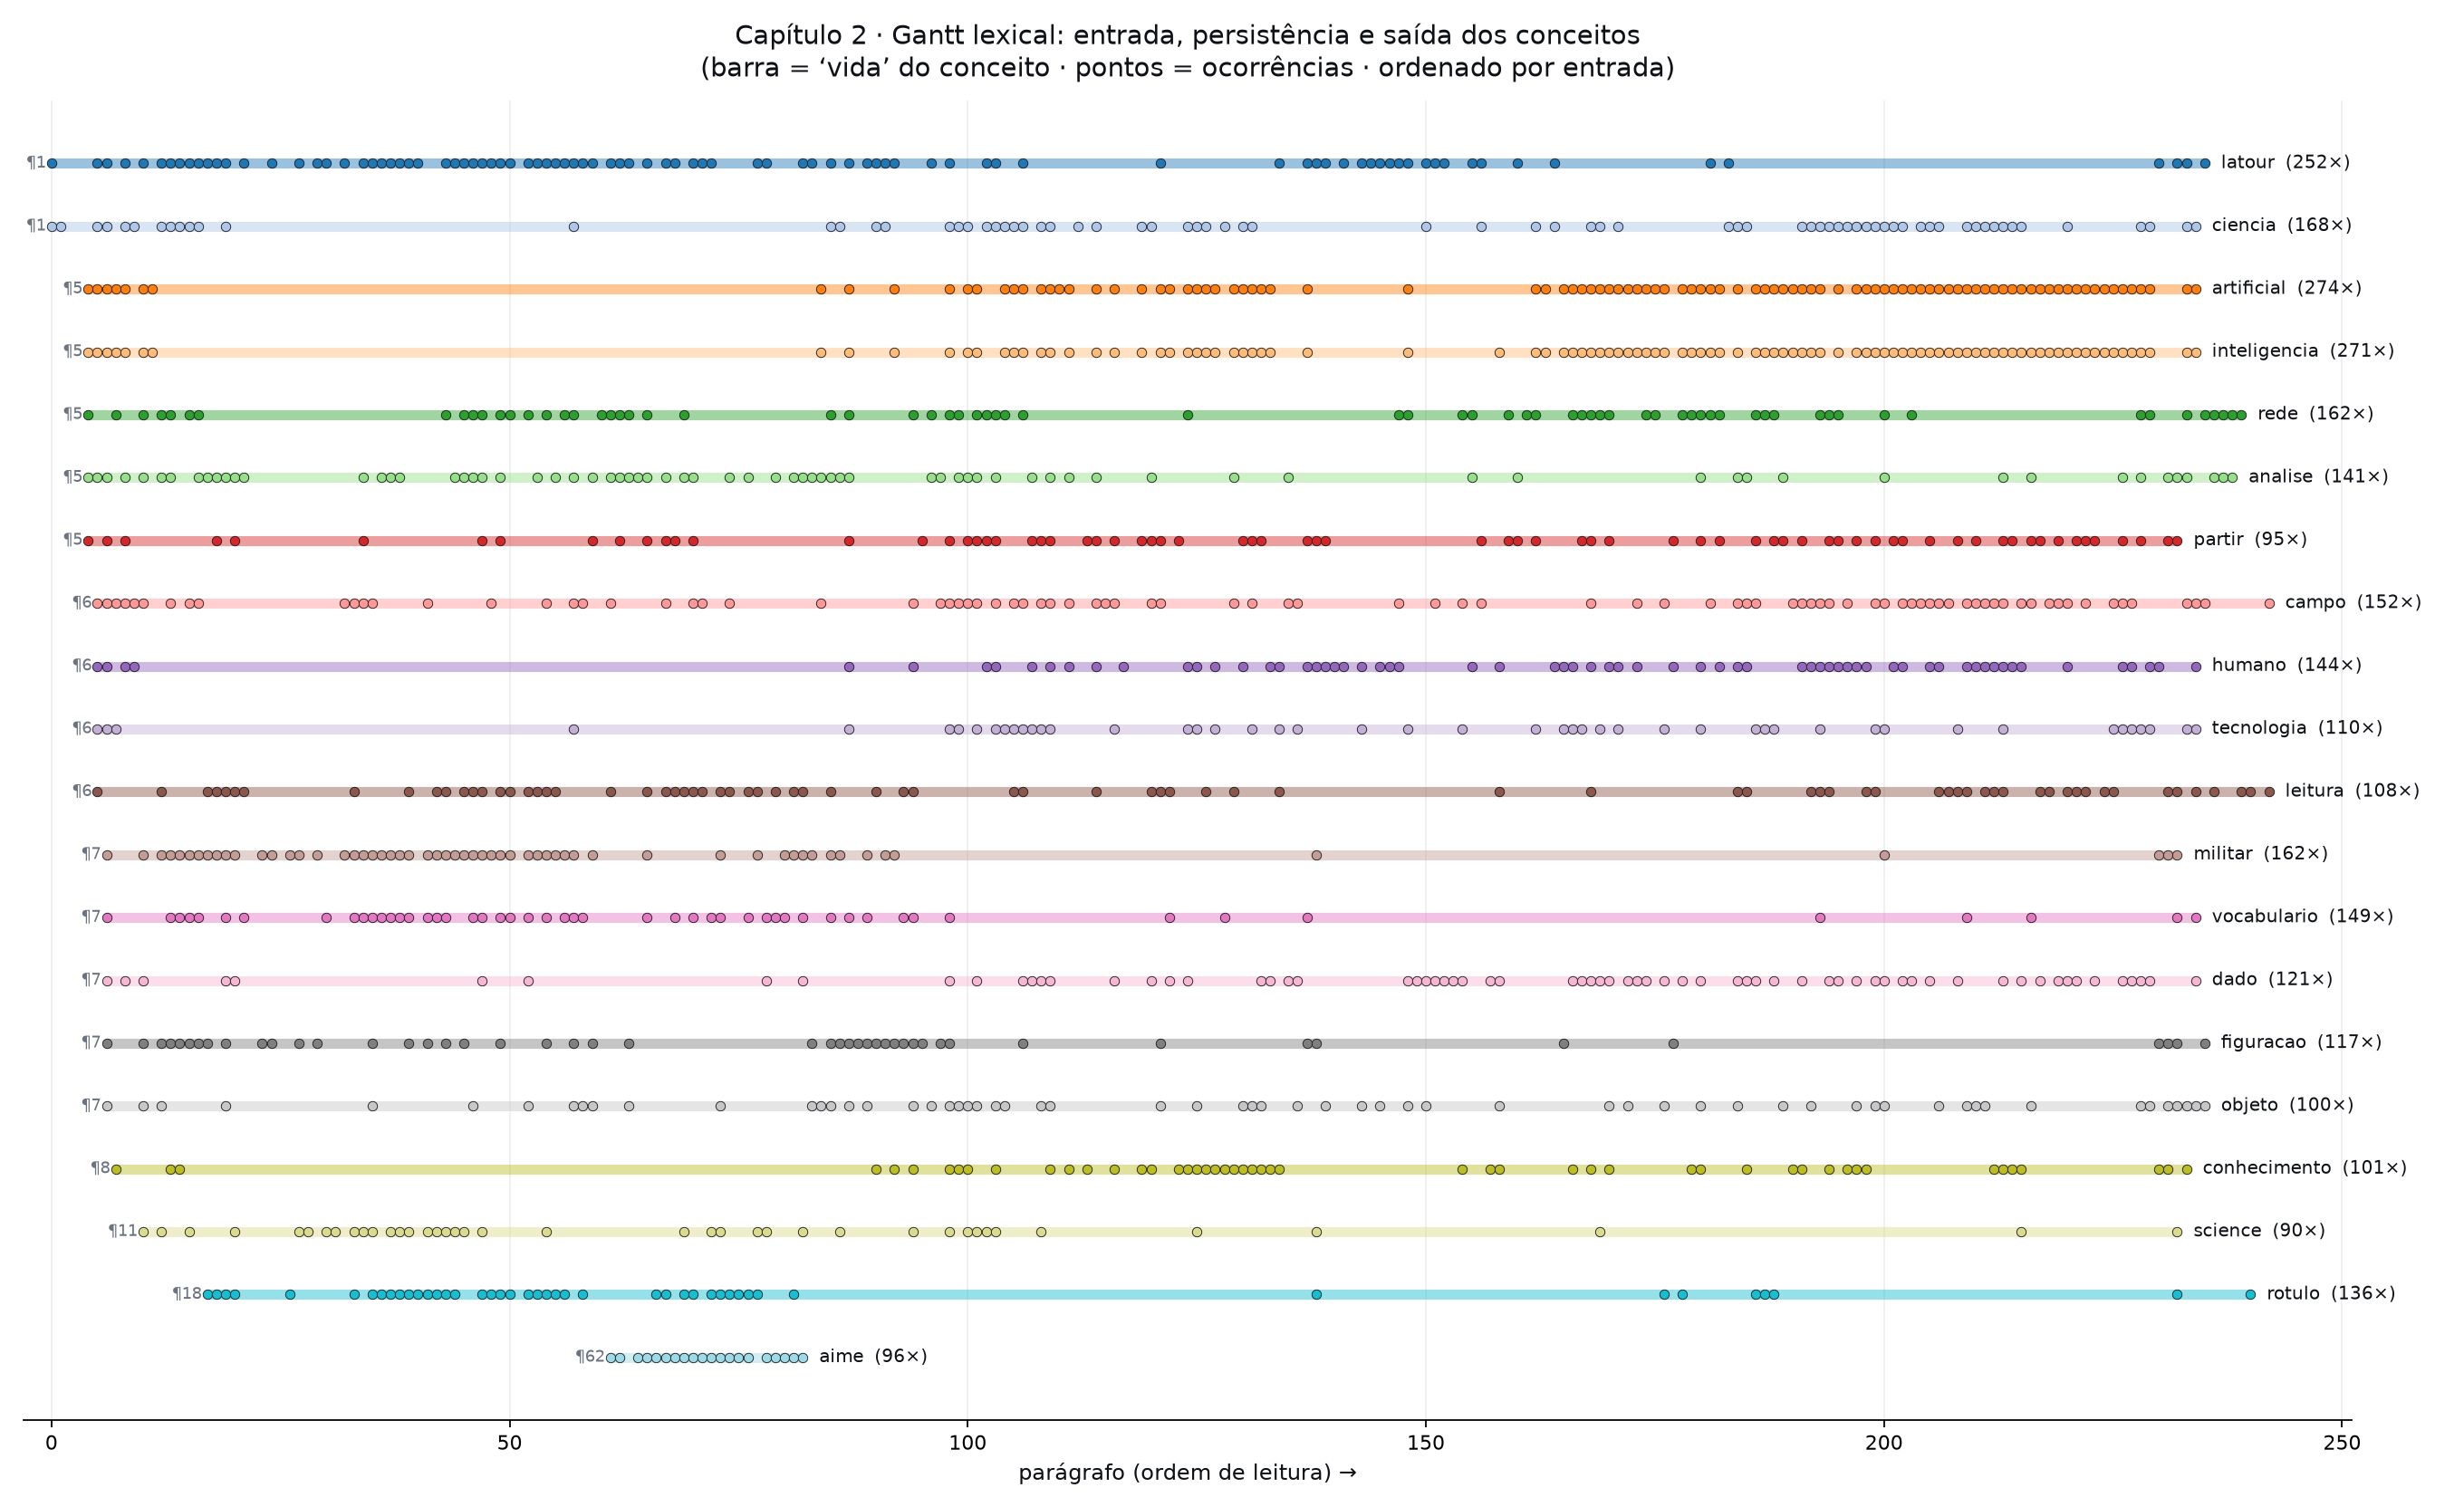
\includegraphics[width=1.0\textwidth,keepaspectratio]{figuras/cap.2/trajectory_gantt.png}
\caption[Gantt lexical do capítulo~\ref{capitulo2}: entrada, persistência e saída dos conceitos]{Gantt lexical do capítulo~\ref{capitulo2}. Cada linha corresponde a um dos 20 conceitos de maior frequência, excluídos termos genéricos e o marcador \texttt{claude}; o eixo horizontal é a ordem de leitura em parágrafos. A barra colorida marca a vida do conceito no capítulo, do parágrafo de primeira aparição (rótulo \P\textit{n}) ao último; os pontos sobre a barra indicam cada ocorrência; o número entre parênteses à direita é a contagem total. As linhas estão ordenadas por parágrafo de entrada, evidenciando a sequência em que cada noção é convocada e por quanto tempo permanece em circulação. Gerado pelo \textit{script} \texttt{narrative\_trajectory.py}, disponível em \url{https://github.com/julianehelanski/tecno-etnografia-centro-ia/tree/main/infranodus}.}
\label{fig:trajectory-cap2-gantt}
\end{figure}

\begin{figure}[H]
\centering
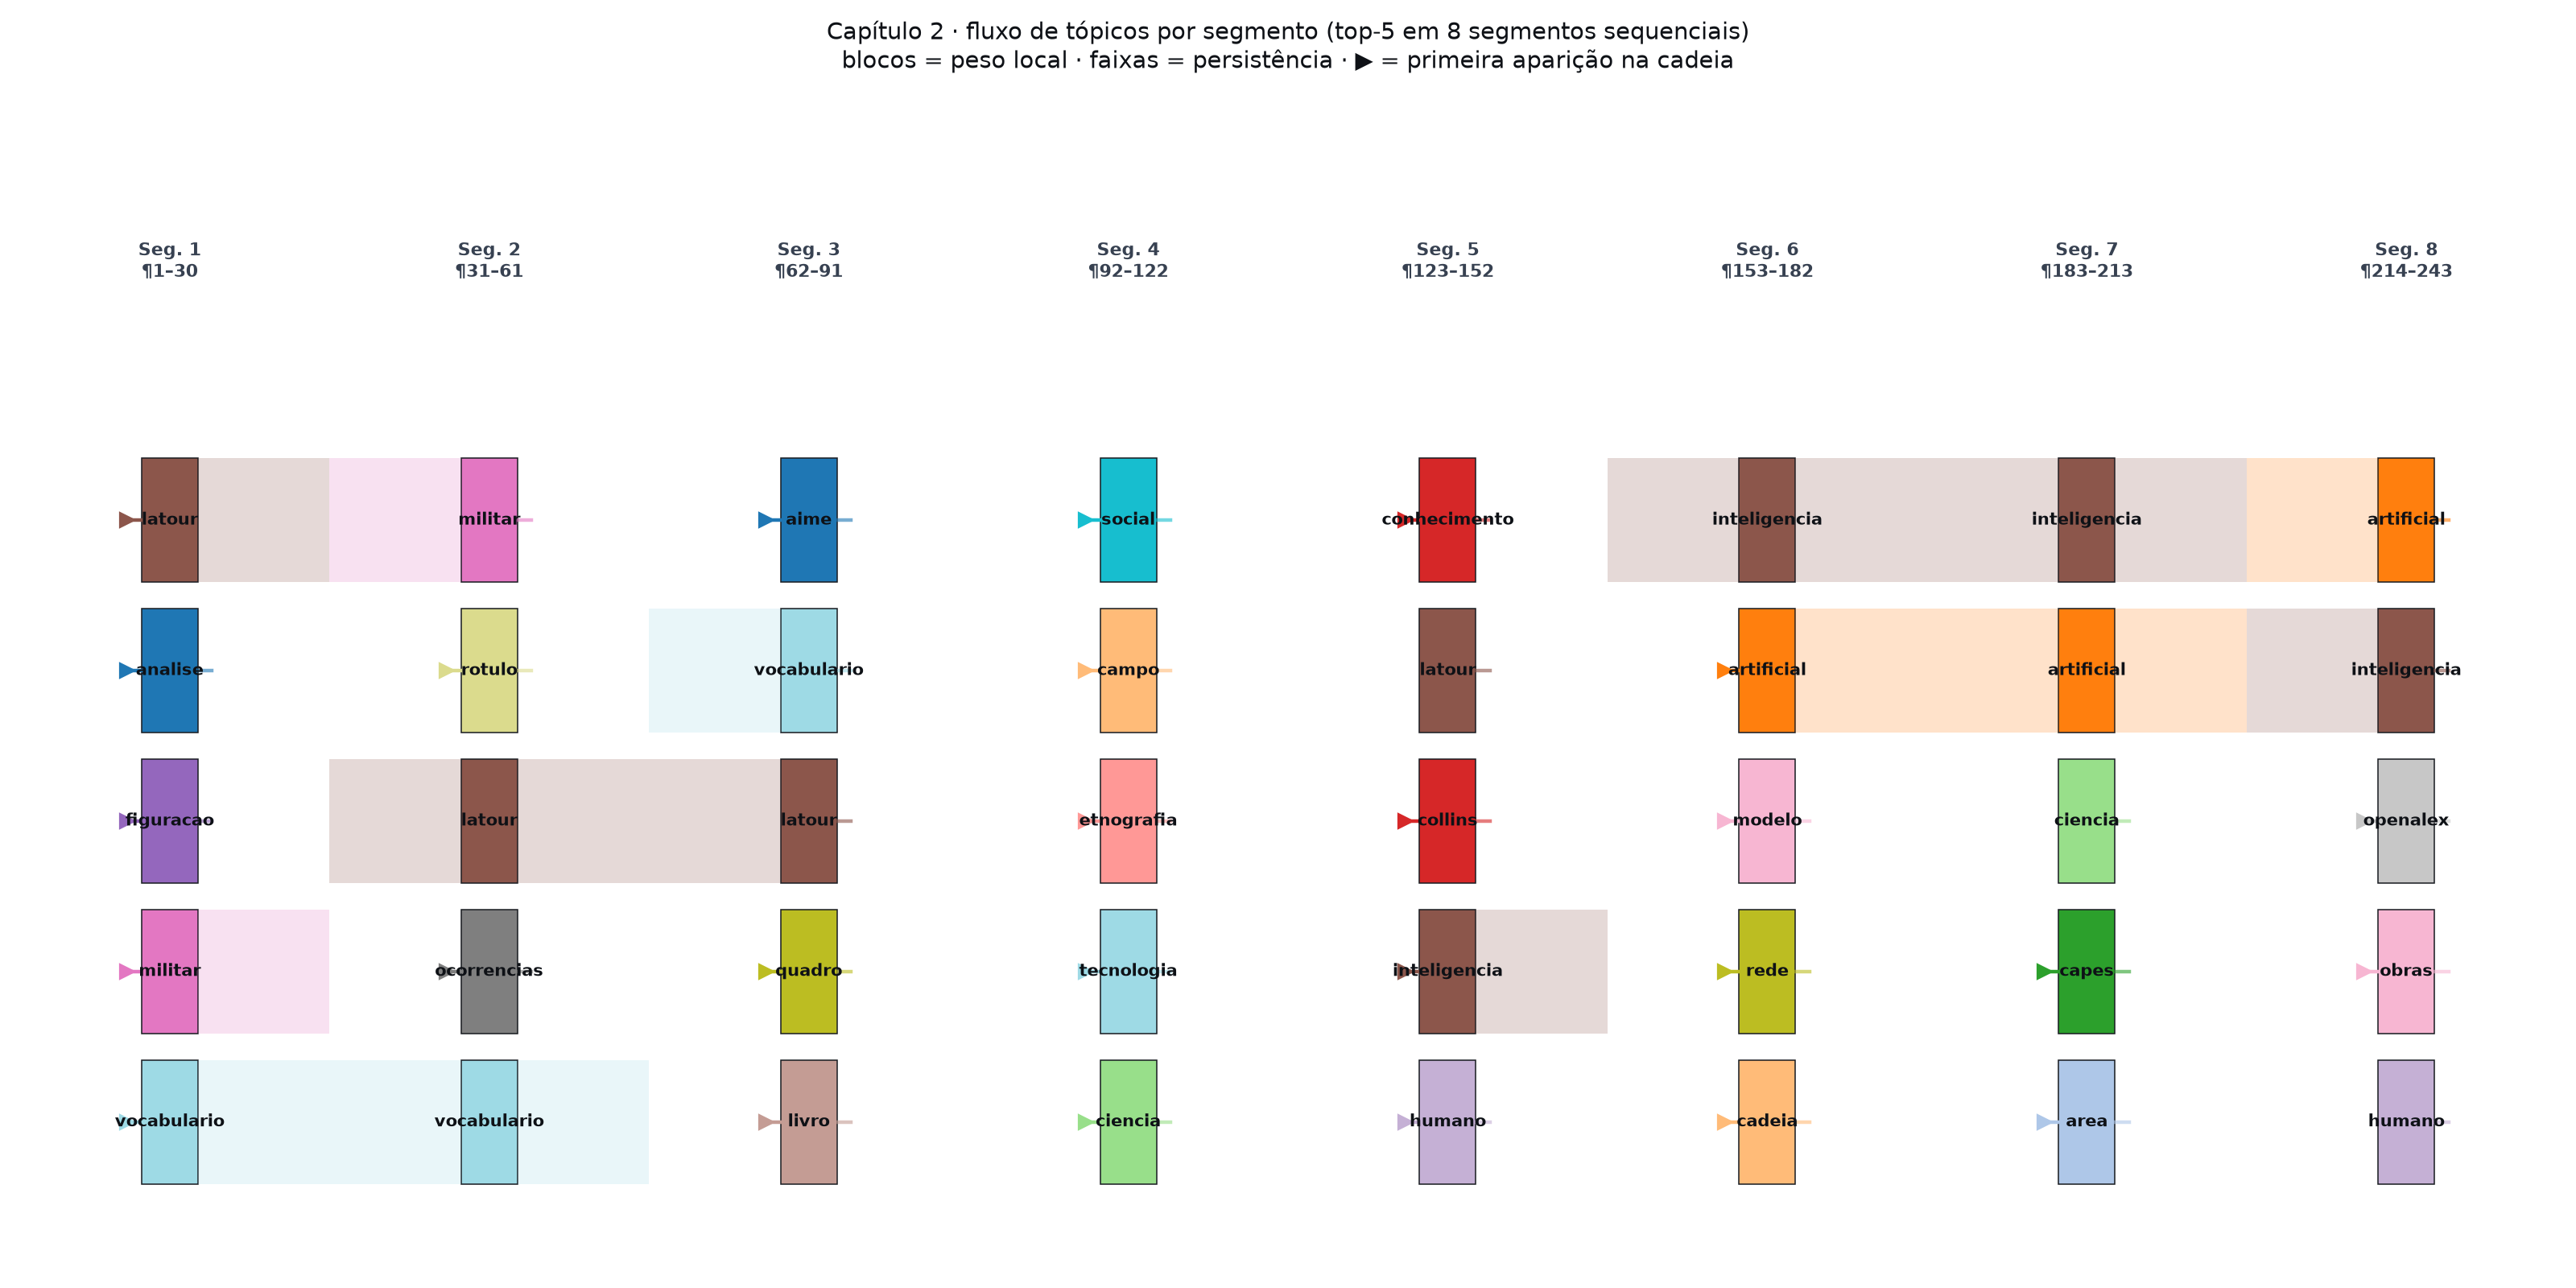
\includegraphics[width=1.0\textwidth,keepaspectratio]{figuras/cap.2/trajectory_alluvial.png}
\caption[Fluxo aluvial de tópicos ao longo do capítulo~\ref{capitulo2}]{Fluxo aluvial do capítulo~\ref{capitulo2}. O capítulo é particionado em 8 segmentos sequenciais de igual extensão em parágrafos (rótulos \P\textit{n}--\P\textit{m} no topo); em cada segmento são listados os 5 termos de maior frequência local (blocos coloridos, com a posição vertical refletindo o \textit{ranking} dentro do segmento). Faixas translúcidas conectam um termo a si mesmo entre segmentos adjacentes quando ele persiste no \textit{top}-5, materializando continuidades temáticas; setas $\blacktriangleright$ assinalam a primeira aparição de um conceito na cadeia. A figura responde à pergunta \enquote{o que se liga a quê ao longo do capítulo} e torna visíveis tanto os tópicos persistentes quanto as entradas tardias e saídas precoces. Gerado pelo \textit{script} \texttt{narrative\_trajectory.py}, disponível em \url{https://github.com/julianehelanski/tecno-etnografia-centro-ia/tree/main/infranodus}.}
\label{fig:trajectory-cap2-alluvial}
\end{figure}

\begin{figure}[H]
\centering
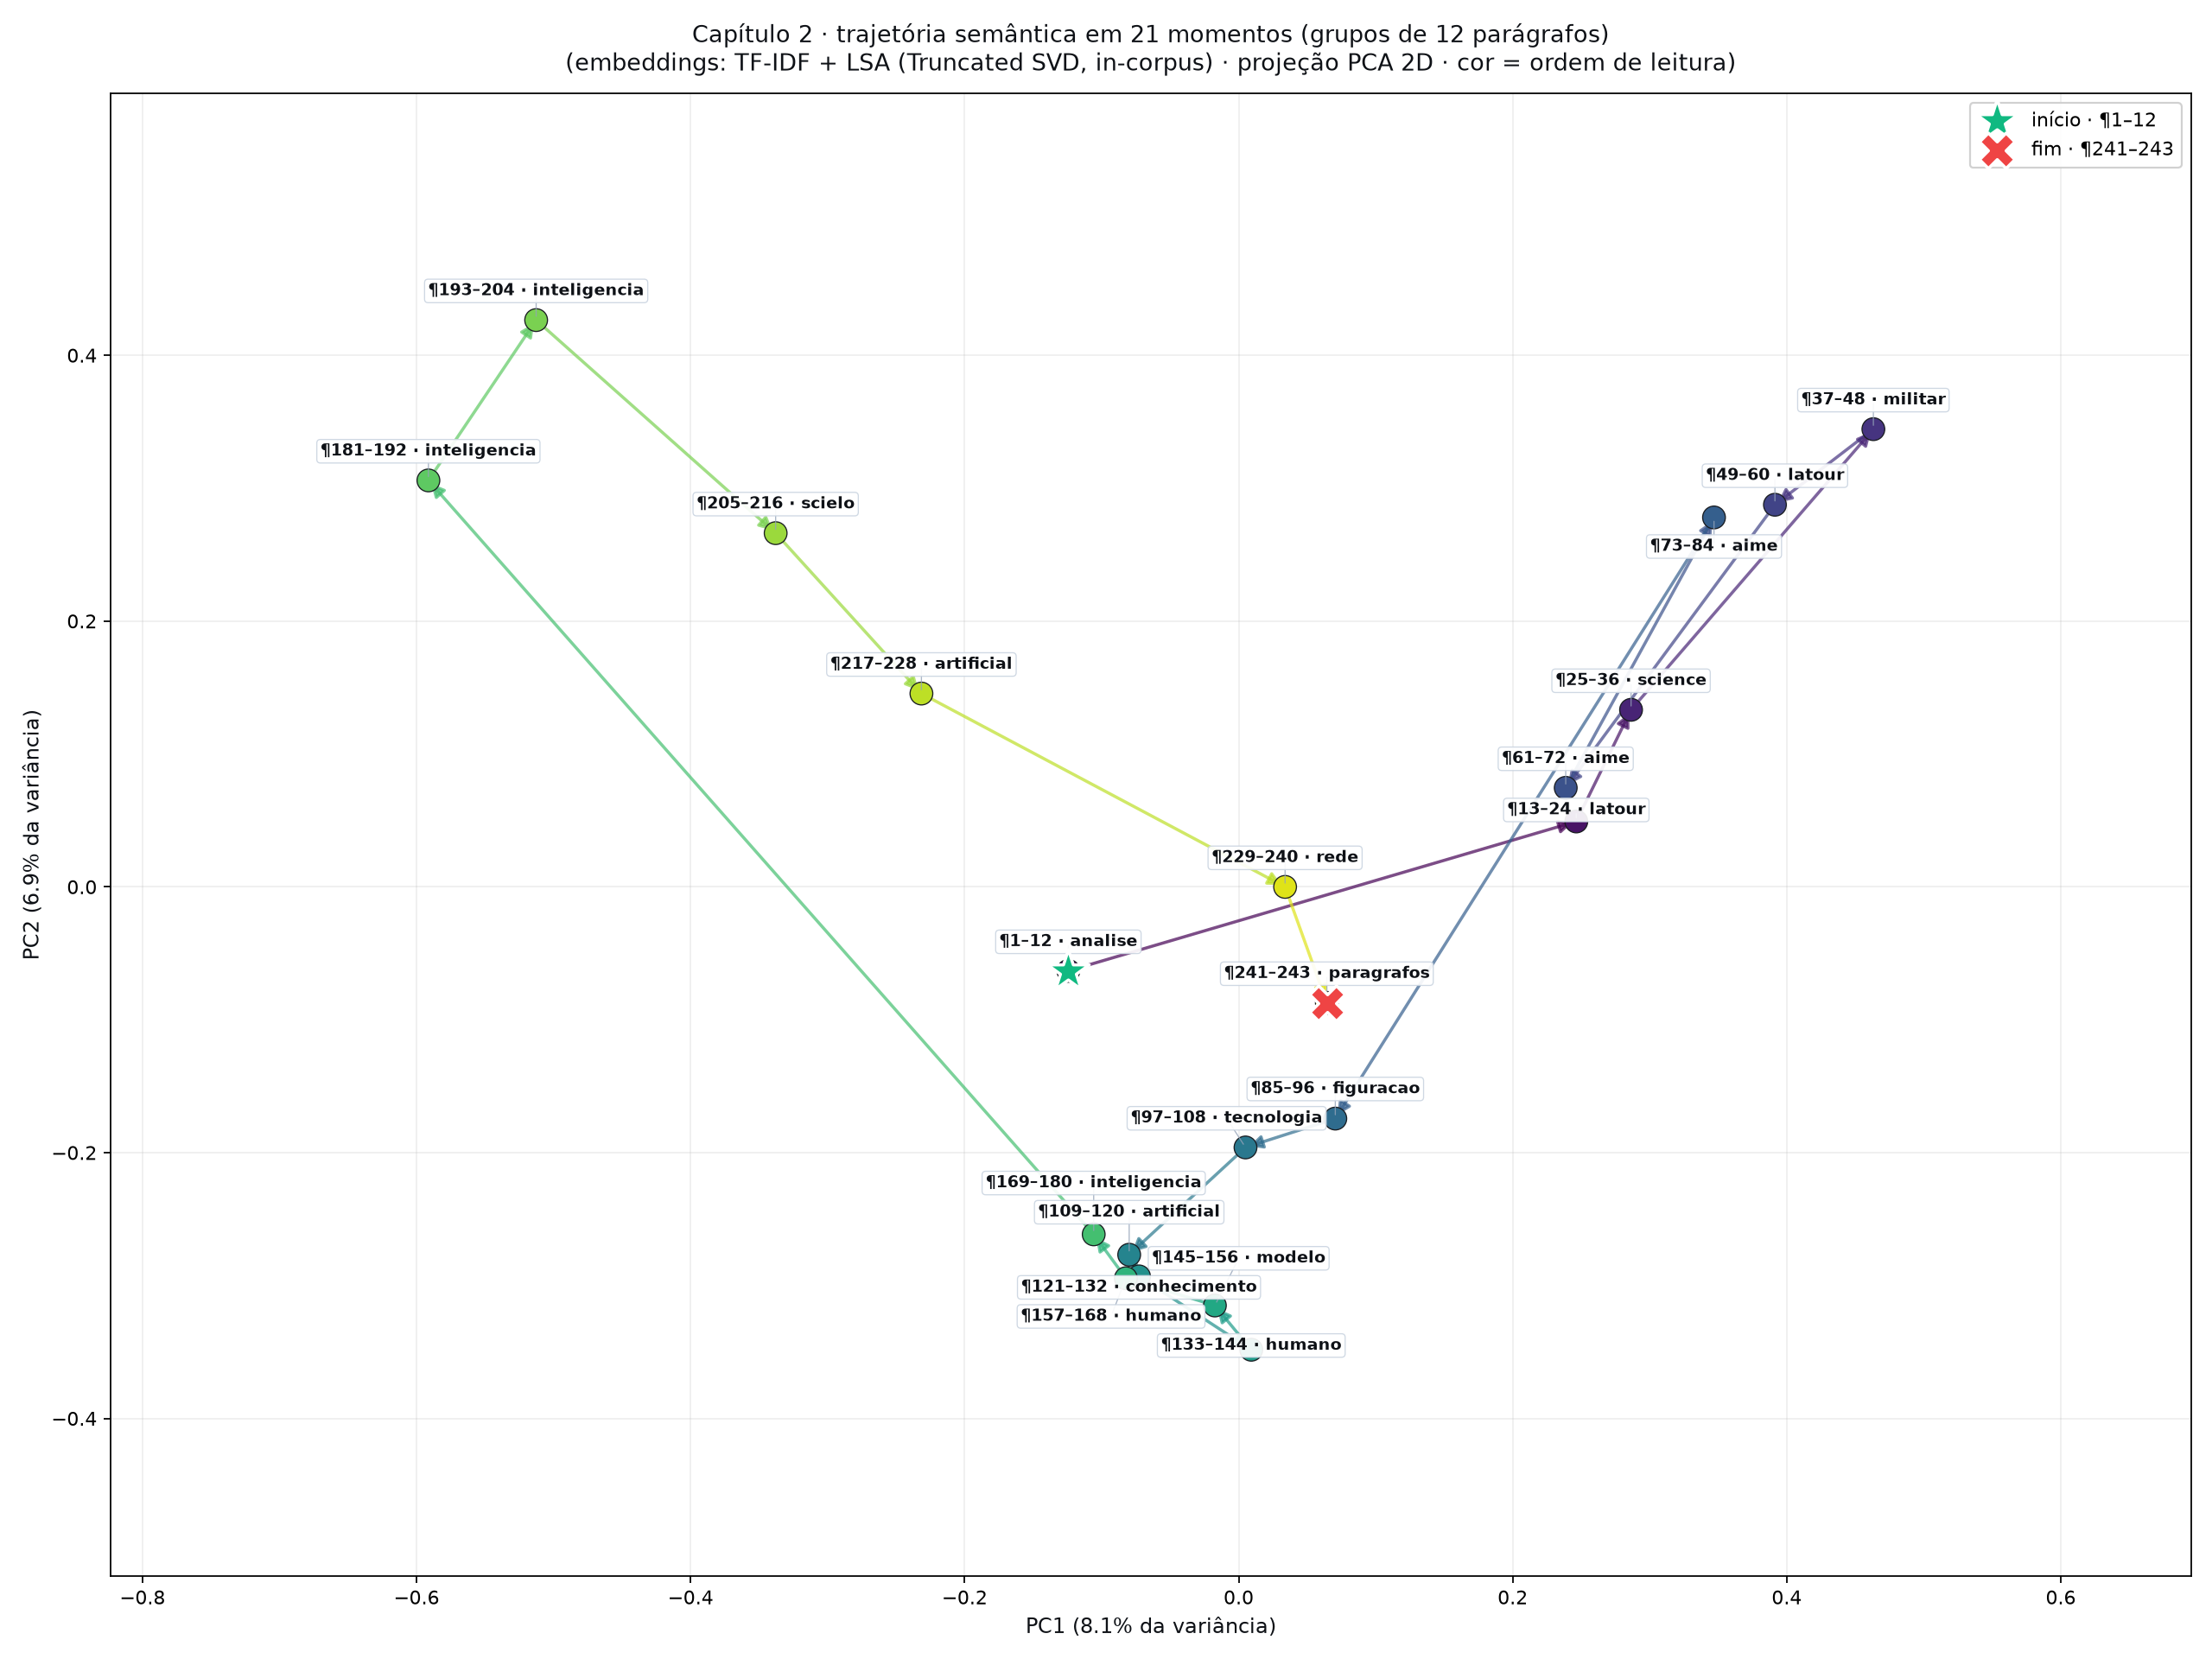
\includegraphics[width=1.0\textwidth,keepaspectratio]{figuras/cap.2/trajectory_semantic.png}
\caption[Trajetória semântica do capítulo~\ref{capitulo2}]{Trajetória semântica do capítulo~\ref{capitulo2}. Os parágrafos são agrupados em \textit{momentos} de 5 parágrafos consecutivos; cada momento é vetorizado por \textit{TF-IDF} (unigramas e bigramas) seguido de redução por \textit{Truncated SVD} (\textit{Latent Semantic Analysis} \textit{in-corpus}, \textit{fallback} usado quando o \textit{sentence-transformer} multilíngue não está disponível) e projetado em duas dimensões por PCA. Cada ponto é um momento, rotulado com o intervalo de parágrafos e o termo dominante; as setas seguem a ordem de leitura, com gradiente \textit{viridis} do início ($\star$ verde) ao fim ($\times$ vermelho). Distâncias no plano aproximam dissimilaridade lexical entre momentos; deslocamentos longos indicam mudanças temáticas, voltas curtas indicam retomada de campo semântico já visitado. O percentual de variância explicada por cada eixo aparece nos rótulos. Gerado pelo \textit{script} \texttt{narrative\_trajectory.py}, disponível em \url{https://github.com/julianehelanski/tecno-etnografia-centro-ia/tree/main/infranodus}.}
\label{fig:trajectory-cap2-semantic}
\end{figure}